% \documentclass[12pt]{scrreprt}
\documentclass[12pt,lot, lof]{outhesis}
% \setcounter{tocdepth}{3}
\setcounter{secnumdepth}{2}
%%%%%%%%%%%%%%%%%%%%%%%%%%%%%%%%%%%%%%%%%%%%%%%%%%%%%%%%%%%%%\
%%%% Use packages (add here your additional packages)
% include bibliography in TOC
\usepackage[nottoc]{tocbibind}

%\usepackage{amsfonts}

%%% For figures
\usepackage{graphicx}
%\usepackage{subfig,rotate}

%%% for comments
\usepackage{verbatim}

%%% For tables
\usepackage{multirow}
% Longtable lets you have tables that span multiple pages.
\usepackage{longtable}
\usepackage{tabularx}
\usepackage{colortbl}
\usepackage{xcolor}
% \usepackage{adjustbox}
\usepackage[graphicx]{realboxes}
\usepackage{trimclip}

% for graphviz
\usepackage[pdf]{graphviz}
\newcommand{\gvnewline}{\noexpand\n} % to type \n in graphviz

% for scientific notation
\usepackage{siunitx}

% https://tex.stackexchange.com/questions/157389/how-to-center-column-values-in-a-table
\usepackage{array}
\newcolumntype{P}[1]{>{\centering\arraybackslash}p{#1}}

% Booktabs produces far nicer tables than the standard LaTeX tables.
%   see: http://en.wikibooks.org/wiki/LaTeX/Tables
\usepackage{booktabs}

%set parameters for longtable:
% default caption width is 4in for longtable, but wider for normal tables
\setlength{\LTcapwidth}{\textwidth}



%%%% End packages
%%%%%%%%%%%%%%%%%%%%%%%%%%%%%%%%%%%%%%%%%%%%%%%%%%%%%%%%%%%%%\


%%%%%%%%%%%%%%%%%%%%%%%%%%%%%%%%%%%%%%%%%%%%%%%%%%%%%%%%%%%%%\
%%%% other stuff (better to not change)

\newcommand{\proquestmode}{}
% I prefer proquestmode to be off for electronic copies for normal use, since the colored links are less distracting. However when printed in black and white, the colored links are difficult to read. 


% Alter some LaTeX defaults for better treatment of figures:
% See p.105 of "TeX Unbound" for suggested values.
% See pp. 199-200 of Lamport's "LaTeX" book for details.
%   General parameters, for ALL pages:
\renewcommand{\topfraction}{0.85}	% max fraction of floats at top
\renewcommand{\bottomfraction}{0.6}	% max fraction of floats at bottom
%   Parameters for TEXT pages (not float pages):
\setcounter{topnumber}{2}
\setcounter{bottomnumber}{2}
\setcounter{totalnumber}{4}     % 2 may work better
\setcounter{dbltopnumber}{2}    % for 2-column pages
\renewcommand{\dbltopfraction}{0.66}	% fit big float above 2-col. text
\renewcommand{\textfraction}{0.15}	% allow minimal text w. figs
%   Parameters for FLOAT pages (not text pages):
\renewcommand{\floatpagefraction}{0.66}	% require fuller float pages
% N.B.: floatpagefraction MUST be less than topfraction !!
\renewcommand{\dblfloatpagefraction}{0.66}	% require fuller float pages

% The documentclass already sets parameters to make a high penalty for widows and orphans. 


%%%%%%%%%%%%%%%%%%%%%%%%%%%%%%%%%%%%%%%%%%%%%%%%%%%%%%%%%%
%%% Printed vs. online formatting
\ifdefined\printmode

% Printed copy
% url package understands urls (with proper line-breaks) without hyperlinking them
\usepackage[hyphens]{url}


\else
\usepackage[hyphens]{url}
\ifdefined\proquestmode
%ProQuest copy -- http://www.princeton.edu/~mudd/thesis/Submissionguide.pdf

% ProQuest requires a double spaced version (set previously). They will take an electronic copy, so we want links in the pdf, but also copies may be printed or made into microfilm in black and white, so we want outlined links instead of colored links.
\usepackage{hyperref}
\hypersetup{bookmarksnumbered}

% copy the already-set title and author to use in the pdf properties
\makeatletter
\hypersetup{pdftitle=\@title,pdfauthor=\@author}
\makeatother

\else
% Online copy

% adds internal linked references, pdf bookmarks, etc

% turn all references and citations into hyperlinks:
%  -- not for printed copies
% -- automatically includes url package
% options:
%   colorlinks makes links by coloring the text instead of putting a rectangle around the text.
\usepackage{hyperref}
\hypersetup{colorlinks,bookmarksnumbered}

% copy the already-set title and author to use in the pdf properties
\makeatletter
\hypersetup{pdftitle=\@title,pdfauthor=\@author}
\makeatother

% make the page number rather than the text be the link for ToC entries
%\hypersetup{linktocpage}
\fi % proquest or online formatting
\fi % printed or online formatting


%%%%%%%%%%%%%%%%%%%%%%%%%%%%%%%%%%%%%%%%%%%%%%%%%%%%%%%%%%%%%\
%%%% Define commands

% Define any custom commands that you want to use.
% For example, highlight notes for future edits to the thesis
%\newcommand{\todo}[1]{\textbf{\emph{TODO:}#1}}


% create an environment that will indent text
% see: http://latex.computersci.org/Reference/ListEnvironments
% 	\raggedright makes them left aligned instead of justified
\newenvironment{indenttext}{
    \begin{list}{}{ \itemsep 0in \itemindent 0in
    \labelsep 0in \labelwidth 0in
    \listparindent 0in
    \topsep 0in \partopsep 0in \parskip 0in \parsep 0in
    \leftmargin 1em \rightmargin 0in
    \raggedright
    }
    \item
  }
  {\end{list}}

% another environment that's an indented list, with no spaces between items -- if we want multiple items/lines. Useful in tables. Use \item inside the environment.
% 	\raggedright makes them left aligned instead of justified
\newenvironment{indentlist}{
    \begin{list}{}{ \itemsep 0in \itemindent 0in
    \labelsep 0in \labelwidth 0in
    \listparindent 0in
    \topsep 0in \partopsep 0in \parskip 0in \parsep 0in
    \leftmargin 1em \rightmargin 0in
    \raggedright
    }

  }
  {\end{list}}



%%%%%%%%%%%%%%%%%%%%%%%%%%%%%%%%%%%%%%%%%%%%%%%%%%%%%%%%%%%%%\
%%%% Front-matter


% For early drafts, you may want to disable some of the frontmatter. Simply change this to "\ifodd 1" to do so.
\ifodd 0
% front-matter disabled while writing chapters
\renewcommand{\maketitlepage}{}
\renewcommand*{\makecopyrightpage}{}
\renewcommand*{\makeabstract}{}

% you can just skip the \acknowledgements and \dedication commands to leave out these sections.

\else


\abstract{
% Abstract can be any length, but should be max 350 words for a Dissertation for ProQuest's print indicies (150 words for a Master's Thesis) or it will be truncated for those uses.
% intro, problem
% ORIENTATION: wider context
% News media is the way that we get informed about information every day.
% We read the news to know what happens and when we do that, not only do we receive the facts, but also the interpretation of the writer.
% that can be distinguished with different degrees of difficulty.
% This phenomenon is called \emph{framing} and different works have analysed it.
In recent years, computational studies started analysing several aspects of News Media.
% Both researchers and private companies, driven by the need to understand and keep a healthy environment around public discussion, began
The research community began
developing models to extract and classify news articles in multiple dimensions: parallel news reports analysis, persuasion techniques detection, political leaning recognition and topic detection.

% RATIONALE: create a niche
While there is a lot of computational research on persuasion detection, we find that it has not been studied together with the other factors of 
%But computational studies lack a study of the relationships between these multiple factors of 
parallel news reports, political leaning, and topics.
% It is important to study the relationship between these factors in order to have a much clearer understanding of propaganda in different conditions.
% With this PhD, we want to tackle instances of framing that are difficult to recognise.
% These can manifest subtly through word choices and selection of what to include or exclude from the narrative line.
%
%
% AIM: purpose of research
% This PhD aims to analyse the relationship between propaganda and parallel news reports, political leaning and topics. We want to understand how propaganda changes across political leaning and topics.
This PhD analyses the use of language in parallel news articles to understand how persuasion changes across political leaning and topics.


% METHOD: methodology and theoretical framework 
We use two methodologies in our work:
(i) comparative analysis: we study one observed dimension across one or more partitioning variables;
(ii) classifier-based: we combine different variables as features for a classifier that needs to predict one additional variable.
With these two methodologies, we analyse how persuasion changes across leanings and topics, and we see what is the effect of using persuasion and topics to predict the political leaning of news articles. 


% contributions
% FINDINGS: outline of the findings
Our work has three main contributions.
(i) We improve the F1 of a political leaning classifier using the features of propaganda and topic.
(ii)
%We quantify the relationships between propaganda and similarities, political leaning and topics. 
We discover that for specific topics, news sources use very different propaganda terms across the political spectrum, while still using the same techniques.
% The same persuasion techniques are used for each topic, even when the political leaning of the article is different.
(iii) We discover an imbalance in the standard datasets for propaganda detection, which raises questions about the generality of results in the literature.
% We present a method that could help both human readers and automated approaches to find more easily when such framing techniques occur in the news.
% We want to provide an analysis of articles, by exploiting the differences in how information is presented by different sources.
% We can then analyse how different sources in the media landscape are using framing in different ways.  


% INTERPRETATION: general significance of the findings 
We believe that the results of this work can be useful both for computational researchers and users reading the news.
For the first group, we emphasise the need to exploit the relationships discovered to improve models (using mixed features) and datasets (making them more representative of the news as a whole).
% For the second group, our work can be applied to build tools to empower the reasoning of users, by letting them compare multiple articles on the same topic and highlighting the techniques used.
For the second group, our work can be applied to build tools to help users compare multiple articles on the same topic, to highlight any techniques used.

}

\acknowledgements{
%I would like to thank...
Above all, I want to express my gratitude to my supervisors, Prof. Harith Alani and Dr. Alistair Willis, for their unwavering support and guidance throughout my research. They were always available to discuss any problems or inquiries I had and provided valuable feedback.
I would like to give a special thanks to Prof. Harith Alani for his thought-provoking questions that helped me stay on track with my research. His talent for simplifying complex ideas into understandable concepts demonstrated that every problem can be solved with the proper approach and clear explanations.
I am grateful for the technical assistance provided by Dr. Alistair Willis, which enabled me to effectively frame and focus the most intricate section of my thesis. Through his invaluable support, I gained valuable insight into designing strong experiments and critically analysing results.

% guidance showed me the importance of good writing in research. Hopefully, his ability to spot the smallest typos and grammatical errors made me a better writer.

I would like to express my gratitude to my friends and colleagues at the Knowledge Media Institute (KMi), Computing \& Communications (C\&C) and generally in the Open University family, for their support throughout my studies. Their assistance has been invaluable to me. Paula, Angel, Angelo, Lucas, Lara, Alba, Agnese, Gianluca, Perla, Tommy, Pedro, Thais, Patrizia, Julian, Miriam, Cecilia and Paco: you all contributed to making life in Milton Keynes better.

And thanks to the two musical bands that accompanied me during this 3-year period, \emph{KMinstruments} and \emph{I Gabbiani}, that provided a good and motivating distraction and made the time more enjoyable. 

Finally, I would like to thank my mum, dad, brother, and sister for supporting me even in the distance over all these years, and spurring me to continue.% and not give up.

Last but not least, I would like to thank Giorgia.
%for her unofficial supervising abilities and for standing on my side.
%and motivation to push me all the times I lost my energy.
Your support has been an inexhaustible source of comfort and motivation for me in all the tough times. Your positive energy and determined encouragement always kept me going, even when things seemed impossible. Your ability to put things into perspective, and focus on the finish line, helped me remain determined and focused on my goals. I am truly grateful for your persistent support and will always cherish it.

%Her ability to deal with a PhD researcher, stressed and anxious about the experiments failing and this never-ending thesis, cannot be expressed in words.

}

\dedication{
Dediction
}

\fi  % disable frontmatter


%%%%%%%%%%%%%%%%%%%%%%%%%%%%%%%%%%%%%%%%%%%%%%%%%%%%%%%%%%%%%\
%%%% Hide some chapters

%%% If you want to produce a pdf that includes only certain chapters, specify them with includeonly, in addition to including all chapters below.
%\includeonly{ch-intro/chapter-intro}
%%% You can also specify multiple chapters.
%\includeonly{ch-intro/chapter-intro,ch-usage/chapter-usage}
%\includeonly{chap1,chap2,chap3}



% template inspired from https://www.overleaf.com/learn/latex/How_to_Write_a_Thesis_in_LaTeX_(Part_1):_Basic_Structure

% \usepackage[utf8]{inputenc}
\usepackage{graphicx}

% for layout
% \usepackage[a4paper,width=150mm,top=25mm,bottom=25mm,bindingoffset=6mm]{geometry}
% \usepackage{fancyhdr}
% \pagestyle{fancy} % adding header to pages
\newsavebox{\largestimage} % for the title_page

% for figures
\usepackage{caption}
\usepackage{subcaption}

% for references
% \usepackage{biblatex}
% \usepackage[natbib=true]{biblatex}
% \addbibresource{references.bib}
% \usepackage{biblatex}
\usepackage{bibentry}
\nobibliography*



% math parentheses
\usepackage{braket}

\usepackage{enumitem}
\setlist[itemize,enumerate,description]{noitemsep,nolistsep} % removes ugly separation of itemize


\usepackage[textwidth=2.2cm]{todonotes}
% default inline todos
% \presetkeys%
%     {todonotes}%
%     {inline,backgroundcolor=orange}{}
% \makeatletter
% \xpatchcmd{\@todo}{\setkeys{todonotes}{TODO: #1}}{\setkeys{todonotes}{inline,#1}}{}{}
% \makeatother
% \let\tododefault\todo
% \renewcommand{\todo}[2][]{\tododefault[inline,#1]{#2}}
\NewCommandCopy{\tododefault}{\todo}
\renewcommand{\todo}[2][]{\tododefault[inline,#1]{TODO: #2}}
\newcommand{\todomargin}[2][]{\tododefault[size=\tiny]{#2}}
\newcommand{\todoAW}[2][]{\tododefault[color=purple,size=\tiny]{AW: #2}}
\newcommand{\todoHA}[2][]{\tododefault[color=red,size=\tiny]{HA: #2}}
\newcommand{\todoHAinline}[2][]{\tododefault[color=red,inline]{HA: #2}}
\newcommand{\todoAWinline}[2][]{\tododefault[color=purple,inline]{AW: #2}}



% status indicators for sections
\usepackage[outline]{contour}
\usepackage{bbding}


\ifodd 0
    \newcommand{\statusgreen}{}%
    \DeclareRobustCommand{\statusgreen}{%
      % \tikz\fill[scale=0.5, color=green]
      % (0,.35) -- (.25,0) -- (1,.7) -- (.25,.20) -- cycle;%
      \textcolor{green}{\CheckmarkBold}
    }
    \newcommand{\statusorange}{}%
    \DeclareRobustCommand{\statusorange}{%
      % \textcolor{orange}{\textbf{$\sim$}}
      % \contour{orange}{\textcolor{orange}{\textbf{$\sim$}}}
      \textcolor{orange}{\HandPencilLeft}
    }
    \newcommand{\statusred}{}%
    \DeclareRobustCommand{\statusred}{%
      % \tikz\fill[scale=0.5, color=red]
      %  (.2,0) -- (.25,0) -- (1,.7) -- (.25,.15) -- cycle;%
      \textcolor{red}{\XSolidBold}
    }
\else
    \newcommand{\statusgreen}{}%
    \DeclareRobustCommand{\statusgreen}{}
    \newcommand{\statusorange}{}%
    \DeclareRobustCommand{\statusorange}{}
    \newcommand{\statusred}{}%
    \DeclareRobustCommand{\statusred}{}
\fi





\graphicspath{ {images/} }

% for \thetitle \theauthor \thedate
\usepackage{titling}

% document properties
% \title{Thesis Title}
% % \subtitle{Subtitle}
% \author{Martino Mensio}
% \date{\today}
%%%%%%%%%%%%%%%%%%%%%%%%%%%%%%%%%%%%%%%%%%%%%%%%%%%%%%%%%%%%%\
%%%% Author & title page info

% \title{Detection of Propaganda across the Political Spectrum\\
\title{Propaganda across the Political~Spectrum\\
\large Quantifying Differences in Parallel News Reports
}

\submitted{September 2023}  % degree conferral date (January, April, June, September, or November)
\date{September 2023}
\copyrightyear{2023}  % year in which the copyright is secured by publication of the dissertation.
\author{Martino Mensio}
\adviserfir{Prof. Harith Alani}  %replace with the full name of your adviser
\advisersec{Dr. Alistair Willis}
%\departmentprefix{Program in}  % defaults to "Department of", but programs need to change this.
\department{Knowledge Media Institute}
\university{The Open University}
%% Full title of the Degree
\degreetitle{Doctor of Philosophy}
% Crest minimum should be 30mm.
\crest{
\includegraphics[width=0.2\textwidth]{images/OU-logo-2017.eps}}
%% College shield [optional] 
% Crest minimum should be 30mm.
\collegeshield{
\includegraphics[width=0.25\textwidth]{images/kmi-logo.eps}}

\usepackage[toc,acronym]{glossaries}

\makeglossaries
\newacronym{kmi}{KMi}{Knowledge Media Institute}

\newglossaryentry{topic}
{
        name=topic,
        description={(wide): topics can be defined in a hierarchy, where top level are very wide (e.g. politics, tech, health, ...).
        (narrow): a set of events that are related, for example that originated from a seminal event}
}
\newglossaryentry{source}
{
        name=source,
        description={A source, or more specifically intended in this work as a \emph{news source} or \emph{news outlet}, is ``anything that provides news information for a period of time is said to be a news source''}
}
\newglossaryentry{event}
{
        name=event,
        description={something that happened in a specific time and place (definition from TDT: http://www.cs.cmu.edu/~nmramesh/p425-nallapati.pdf}
}
\newglossaryentry{seminal-event}
{
        name=seminal event,
        description={an event that is at the start of a set of other events, linked by temporal dependency or causal dependency}
}
\newglossaryentry{story}
{
        name=story,
        description={a news article, that focuses on a main event but also contains references to other events}
}
\newglossaryentry{corroborate}
{
        name=corroborate,
        description={Containing a piece of specific information which is confirmed by other sources. As more sources present the same information, even with slightly different terms, the information shared is \emph{corroborated}}
}
\newglossaryentry{omit}
{
        name=omit,
        description={Not including a piece of specific information, which instead appears in other sources}
}
\newglossaryentry{clique}
{
        name=clique,
        description={The original definition is that of a complete subgraph: every pair of nodes belonging to a clique has an edge that links the two nodes~\citep{luce1949method}. In this work, we use the term \emph{document-level clique} and \emph{sentence-level clique} together with a similarity threshold to indicate a group of documents or sentences that are all similar enough the one to the others. It differs from \emph{clustering} because single nodes do not need to belong to a cluster, they can be on their own.}
}
\newglossaryentry{narrative}
{
        name=narrative,
        description={a particular way of explaining or understanding events 
            https://dictionary.cambridge.org/dictionary/english/narrative
        }
}
\newglossaryentry{propaganda}
{
        name=propaganda,
        description={Use of language that has the specific goal to persuade the reader. It has many points in common with argumentation/rhetorics and is usually associated with deceiving techniques, partial point of views}
}
\newglossaryentry{propaganda-technique}
{
        name=propaganda technique,
        description={One of the practical ways that propaganda uses in language. Many of them in the literature, overlap with logical fallacies. Reference in this work comes from \cite{TODO}, 18 techniques in computational detection}
}
\newglossaryentry{political-leaning}
{
        name=political leaning,
        description={From far left to far right, passing through the centre. In this work it is taken as a wide simplification of political viewpoints}
}

\begin{document}

\begin{titlepage}
% \newgeometry{left=3cm,bottom=0.1cm}
    \begin{center}

        \centering
        \savebox{\largestimage}{
\includegraphics[width=0.2\textwidth]{images/kmi-logo.eps}}
        \usebox{\largestimage}
        \hfill
        \raisebox{\dimexpr.5\ht\largestimage-.5\height}{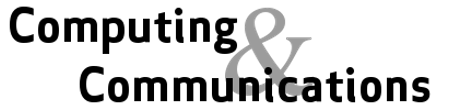
\includegraphics[width=0.2\textwidth]{images/cc_logo.png}}

        \vspace{-1.4cm}
        
\includegraphics[width=0.3\textwidth]{images/OU-logo-2017.eps}
        \vspace{1.6cm}

        % \centering
        % \savebox{\largestimage}{
\includegraphics[width=0.3\textwidth]{images/kmi-logo.eps}}
        % \usebox{\largestimage}
        % \hfill
        % \raisebox{\dimexpr.5\ht\largestimage-.5\height}{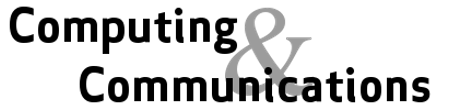
\includegraphics[width=0.4\textwidth]{images/cc_logo.png}}
        
        \vspace*{2cm}
            
        \LARGE
        \textbf{\thetitle}
            
        \vspace{0.5cm}
        \LARGE
        % \makeatletter \@subtitle \makeatother % this needs the scrreprt document class
        \Large 
        \vspace{2cm}
            
        \textbf{\theauthor}
            
        \vfill
            
        This dissertation is submitted for the degree of\\
        \emph{Doctor of Philosophy}

        \vspace{1.5cm}

        % \noindent
        % \begin{tabular*}{\textwidth}{@{\extracolsep{\fill}} l r @{}}
        % \textbf{Advisers}: & \\
        % Prof. Harith Alani & \\
        % Dr. Alistair Willis & \\
        % \end{tabular*}


        \textbf{Advisers}:\\
        Prof. Harith Alani\\
        Dr. Alistair Willis
            
        % \vspace{0.8cm}
            
        
        
        
        
        % \centering
        % 
\includegraphics[width=0.5\textwidth]{images/kmi-logo.eps}
        
        \vspace{1.5cm}
            
        \large
        % Knowledge Media Institute\\
        % The Open University\\
        % United Kingdom\\
        \thedate
            
    \end{center}
    % \restoregeometry
\end{titlepage} % new style
\makefrontmatter % old style: maketitlepage is the title page (outhesis.cls)

% \doublespacing

% \chapter*{Abstract}
% Abstract goes here

% \chapter*{Dedication}
% ...

% \chapter*{Declaration}
% I declare that..

% \chapter*{Acknowledgements}
% I want to thank...

% \tableofcontents
% \listoffigures
% \listoftables

\chapter{\statusgreen Introduction}
\label{chap:intro}

% ROUND 2 comments AW
% \todoAWinline{
% You say at the beginning that you’re going to talk about “persuasion” rather than “propaganda” or “framing”. And then you talk about “propaganda” a lot. Does that need tweaking?
% You give your 4 research hypotheses, but they’re all stated as straight facts, so I can’t work out what the actual hypothesis is. These want rephrasing so that it’s clear what is your hypothesis, and what are the facts which led to the hypothesis. “The first hypothesis is that… . This is based on Bloggs’ (1836) observation that…”
% }


% ROUND 1 comments
% \todoHAinline{Of course, at this stage, we’re not looking for perfection, so I focused more on the parts that are not at a ‘good enough’ level. This is mainly the RQs, and Hypotheses. I made suggestions for each RQ so consider those carefully. Wrt Hypotheses, I would expect them to map directly to your RQs, I think your 3rd H does, but the 1st and 2nd Hs seemed off the mark.
% The other weak part is Motivation. If you have time, try to spin the text around what problem you’re trying to solve or what new knowledge you’re trying to create. Current narrative is about what group of stakeholders you’re trying to benefit. This is generally not the point, and more so when the work does not involve any stakeholder groups; ie no user studies.}
% \todoAWinline{I think the basic content here is fine, but it's really verbose. There are points where what you're saying is confusing, and I suspect it's because you're not getting things sorted out in your own head before typing.
% I'd recommend attempting to reduce what you've written by a third, and that process might reveal how you could express your ideas more concisely.}

% Orientation: wider context

% situation
Thousands of news articles are published every day about the latest events around the world.
The use of specific language, the selection of details, and how the narrative is presented, are all different aspects that are unique to each news outlet and author.
These peculiarities, at the same time, can influence what the reader perceives about the events described.
% framing definition
This whole set of information, whether implicit or explicit, extends the raw facts of the events covered by news articles.
% and are shared as ground truth between multiple sources.
This additional layer, which varies across multiple news reports, comes under different names, such as \emph{framing}~\citep{gamson1989media,scheufele1999framing} or 
%\emph{persuasion}, 
\emph{propaganda}, with slightly different definitions.
For conciseness, in this work we denote these techniques with the single term \emph{persuasion}.
These techniques are often conveyed with subjective statements, mixed with the objective description of the event narrated.
%, but there are also other factors.
%, but not only.
%it does not stop there.
% TODO reference: ``Various observers have noted how subtle framing subtly and unconsciously [framing] operates'' (Gamson and Modigliani, 1989, p. 7)
Even selecting which details or features to report greatly affects the message sent to the reader.

% introduce ideology/leaning
In this landscape of parallel news reports, there are multiple factors in play, such as political orientations and ideologies, that may influence the writing style of news outlets.
For example, persuasion may be used to push for political ideologies directly or indirectly.
% introduce topics
The persuasion used may also change with respect to the \emph{topic} of the news. Some topics are more polarising while others are more neutral.

% EXAMPLE NEEDED HERE

% % example
% For example, taking two sentences ``\textit{the black man was shot}'' vs ``\textit{the man was shot}'', they have a different framing because, although the man shot was black, it is a judgement of the reporter whether this detail needs to be emphasised or not, considering the ethnicity of the person who was shot to be important. %implying a form of racism with respect to a race-independent murder.

% Framing can have a big impact on the way readers perceive the content and relevance of the news~\citep{cohen2015press}. %(\textit{Agenda-setting}).

This thesis explores the relationships between persuasion, political orientation and topics.
These variables are studied independently in the existing literature, and this work aims at understanding the links between them.








% PhD Project done across \acrshort{kmi} and Computing\&Communications.

This chapter contains an introduction to the thesis.
Section~\ref{sec:intro_problem} contains the Problem Statement, Section~\ref{sec:intro_motivation} the Motivation, Section~\ref{sec:intro_rqs} contains all of our Research Questions. Then in Section~\ref{sec:intro_hyp} we present our hypotheses, and in Section~\ref{sec:intro_method} the general methodology used. We end the chapter with the main contributions in Section~\ref{sec:intro_contributions}, %the structure of the dissertation in Section~\ref{sec:intro_structure} 
and our publications in Section~\ref{sec:intro_publications}.


\section{\statusgreen Problem Statement}
\label{sec:intro_problem}


% At the intersection with misinformation, political issues, ...
% Study on propaganda

In this thesis, we analyse persuasion techniques, with a focus on propaganda, to understand how they relate to additional dimensions (topic, leaning, similarity).

To the best of our knowledge, there are hardly any computational studies that analyse the relationship between persuasion means, leaning, topics and similarity.
% This is not a problem on its own, but what is missing is an understanding of how these dimensions interact.
% Acquiring this missing knowledge, we could be able to 

What makes news articles about the same issue different? 
Some studies focus on the information level, by considering which details are included (corroborated) or omitted~\citep{bountouridis2018explaining}.
This is done by comparing multiple parallel articles that cover the same story, and studying what overlaps and what is unique.

Then there is a second branch of research that instead investigates the use of linguistic techniques, such as persuasion, propaganda, sentiment and emotions. This second group tends to focus on single articles analysed on their own, in order to build models to detect such linguistic techniques over news articles~\citep{da2019fine}. %This set of features is considered as a layer of framing/propaganda on top of the facts described,\todoAW{Considered by whom? Don't use the passive!} and it needs to be properly recognised.

Then a third group of works sees the problems by considering only the political leaning. Here we find approaches to recognise political leaning from news articles~\citep{baly2020we}, to provide balanced news feeds to users (e.g. AllSides, Blue Feed - Red Feed), and to label the leanings of news sources (datasets e.g., Media Bias/Fact Check, AllSides).

The final group focuses on topic analysis. Researchers usually employ this method to break down many different types of results, belonging to different tasks and methodologies, to get more fine-grained insights~\citep{zhang2023strategic}.
% TODO: FIND SOME EXAMPLES OF TOPICS ANALYSIS FOR PROPAGANDA, NOT COMPUTATIONAL.
However, there is a lack of computational approaches or analyses that consider the topic as an additional variable to propaganda, leaning or similarity.


Between these multiple branches of research, we see potential links that are left unexplored.
For example, regarding the potential connection between propaganda and leaning, there is a lack in knowledge on \emph{what are the differences in persuasion/propaganda used by different political orientations?} or \emph{How can we automatically recognise political leaning from propaganda?}

% What is the relationship with the topics discussed?
Furthermore, if we consider the relationship between topics and propaganda, it would be useful to understand \emph{which topics tend to attract more propaganda} and \emph{which ones are targets for polarised propaganda}. Adding also the leaning, to \emph{identify topics where propaganda is more distinguishable between political leanings}. 
This would give insights into how propaganda changes across topics and leanings, considering both the quantity and the specific terminology used.
%This would on one side give insights about how the quantity of propaganda changes across topics and leanings, and on the other side about how the terminology used changes across techniques, leanings topics for the specific techniques of techniques used and specific terminology used. 

% \subsection{\statusgreen Key concepts}

% Here we describe the most important concepts that are touched in this thesis. For a complete list, please refer to the Glossary.
% \todoAW{I'm not sure what you're trying to achieve with this list. It feels a bit as though you're just dropping some key terms in, without giving a sense of why they need defining.}
% \todoHA{I think it’s good to provide definitions but I agree that it’s best to drop this section to save time at least. You can put it back if examiners ask for it. I also agree with AW’s comments on each definition.}

% \leftskip=3em
% \parindent=-3em

% \textbf{Event}: \glsdesc*{event}\footnote{\url{https://dictionary.cambridge.org/dictionary/english/event}}.

% \textbf{Parallel News}: \glsdesc*{parallel-news}

% \textbf{Similarity / Variations}: The specific combination of \gls{corroborate}[d] and \gls{omit}[ted] details.\todoAW{Not a sentence.} Terms that change.\todoAW{Not a sentence.} Similarity metrics\todoAW{So is it the details or the metrics? Again, precision!} that score how similar/dissimilar articles are.\todoAW{Not a sentence.}

% \textbf{Persuasion}: \glsdesc*{persuasion}

% \textbf{Propaganda}: \glsdesc{propaganda}

% \textbf{Political Leaning}: \glsdesc{political-leaning}

% \textbf{Topic}: \glsdesc{topic}


% \leftskip=0em
% \parindent 1.5em

\section{\statusgreen Motivation}
\label{sec:intro_motivation}

% % Rationale: create a niche
% % TODO why spotting is useful: http://faculty.sites.uci.edu/polletta/files/2016/02/22A-Simple-Intervention-to-Reduce-Framing-Effects-in-Perceptions-of-Global-Climate-Change22.pdf

% % need of comparing multiple articles
% Spotting the occurrence of framing is therefore a very difficult task, even for humans~\citep{morstatter2018identifying}. Something that could help in this situation is looking at different sources and analysing how they present the same event with different framing.
% By seeing ``the other sides'' of the story, we, as readers, could create a more complete picture and spot the differences at the macro (the perspective of the overall article) and micro-level (specific linguistic cues)~\citep{gamson1989media}.
% The main problem with this technique is that it requires a lot of time,
% and many people only read news articles superficially% very lazy while consuming the news
% ~\citep{pennycook2019lazy}.
% % to read, compare, track, and differentiate all the small details \todo{any citation to support this statement?}.
% % tech limitations
% At the moment, we can see a gap in the tools available to provide this functionality automatically.
% Some technologies analyse parts of the problem, e.g. by grouping articles together by events (news aggregators), or anti-plagiarism tools that spot sentences occurring in multiple documents, or theoretical studies and conceptualisations analysing framing under different aspects.
% But to our knowledge, none of them is bringing together different stories to highlight the framing differences automatically.


% % Aim: purpose of research

% This PhD aims at creating a methodology to extract and characterise framing differences among news articles.
% This includes on one side revealing the choices done by the authors, and bring to the light the types of techniques they use to stand their point of view (e.g., selection and emphasis of details, addition of subjective content).
% And on the other side, to study the information flow between sources and see which relationships exist between them. %(e.g., reusing content).


% Who can find this thesis useful?
% The motivations of this thesis are multiple.

By analysing the relationship between propaganda, political leanings and topics, we aim to understand how strongly they are linked together.
Modelling these factors together could be beneficial in improving the results of tasks that are considered in isolation.
% \todoHA{And what is the motivation behind your need to understand this relationship? What would this lead to, potentially?}
There is a wide literature, both theoretical and practical, about each of these factors.
On the qualitative research level, there are some works that explain and motivate this relationship by analysing a specific event or timeframe~\citep{pierri2023propaganda,golovchenko2020cross,blumberg1986comparative}.
However, on the computational side, we find a lack of approaches that consider these factors together.

A computational approach, which considers together document similarity, propaganda, leaning and topics, would contribute to knowledge in several ways:
% \todoHA{This is ok, but a better narrative would be to focus on where you are advancing knowledge, especially since you did not do any user studies that involved these stakeholders.. if you have time then change the narrative. }

% \todo{Motivation: focus more on advancing knowledge, take the points below and rewrite them to put focus on advancing knowledge}

% \begin{enumerate}
%     \item Computational Researchers:
    \begin{enumerate}
        \item Quantify the relationship between political leaning and propaganda. 
        %The literature assumes %\todoAW{Very vague and sweeping. How would you justify this? (Or refute it?)}
        We find examples in the literature~\citep{schudson2002news} that explain how the political ideology of news writers/editors conditions writing news articles, considering economic reasons, unconscious assumptions and reporter-sources relations that are linked to political leanings. Therefore, these factors result in news articles that contain more or less subtle persuasion techniques for the reader (one of which is propaganda). By analysing and quantifying these relationships, we can understand their importance.
        % contribution 1: compute weights of these relationships, understand better the relationships
        \item By using together these variables, we can try to improve some automated approaches that currently rely on just one input feature, such as political leaning classification
        % \todoHA{so this is the type of value added that I was looking for. If you reach a better understanding of X, then you can improve Y. This could go earlier in this section.}
        using propaganda and topic features. By exploiting the relationship between these features, we can help \acrfull{ml} models to have higher values for the target metrics. % contribution 2: improve F1 using mix of feature
        \item With an analysis that considers multiple variables, we may identify problems and inconsistencies that can only be discovered with combined analyses (e.g., data imbalance). This is a valuable point when using \acrshort{ml}-based approaches, as improving the quality of the data is a key element. % contribution 3: We highlight the problem of imbalanced dataset for propaganda detection
    \end{enumerate}
    % \todoHA{Fits better in a discussion section at the end of the thesis}
%     \item Users reading the news:
%     \begin{enumerate}
%         \item link and show similarities to other documents on how the same topic is covered.\todoAW{Not a sentence} Especially articles from other political leanings which may have a different angle.\todoAW{Not a sentence}
%         \item support with a tool to highlight propaganda, to be conscious of the techniques used in the articles at the word level. It is crucial for this analysis to be as accurate as possible, and that is why we aim to find insights which may help create or extend datasets\todoAW{Isn't the aim to actually do the highlighting? Do you do anything on how to extend datasets?} (e.g., in the case of unbalanced datasets).
%         \item understand better how propaganda distributes across leanings and topics, to be able to recognise more manipulation and be less manipulable.\todoAW{How is this different from the previous point?}
%     \end{enumerate}
% \end{enumerate}


% Motivation/Orientation: multiple narrations of the same events. Driven by multiple factors (selection criteria, point of view of author/publisher, relevance, agenda-setting, …)
% This is linked with Persuasion, but more specifically propaganda. Communication with the goal to persuade. Subtle or more explicit.
% What distinguishes one piece of news from the others about the same event? 

% Political ideology → writer/editor → news (facts + propaganda(opinion)) → persuasion of reader

% Rationale (niche): computational propaganda detection is at an early stage in the research community. Current detection is based on unbalanced datasets that particularly target right-leaning news.

% Aims/Goals of this thesis: 
% understand how propaganda varies across the political spectrum
% Computational perspective: is propaganda detection ready to work in news independently from the political orientation/leaning of the source?




\section{\statusgreen Research Questions}
\label{sec:intro_rqs}

Given this aim, we build a research path that gradually adds the different variables.

\begin{enumerate}
    \item We start from the first factor of similarity (and difference) between news articles, which is the motivation for our work in the first place. Being able to analyse the similarities and differences enables us to get a grasp on what effectively changes between related articles. Therefore, our first \acrfull{rq} is:\\
    \emph{RQ1: To what extent do news articles about the same events differ?}
    \item Then, we move our focus to the computational detection of persuasion techniques. How they can be detected, and what is the relationship to our first \acrshort{rq}1. This prepares us for the second research question: \\
    \emph{\acrshort{rq}2: To what extent can we automatically detect the persuasion techniques used in news articles?} 
    \item Afterwards, we introduce the variable of political leaning, to understand how it relates to persuasion. This leads us to the third research question:\\
    \emph{\acrshort{rq}3: To what extent could the use of persuasion techniques help identify the political leaning of a news article?}
    \item Finally, we introduce the topic as the last variable, to break down the results found in the previous investigation. This is our last research question:\\
    \emph{\acrshort{rq}4: How does the use of propaganda differ across topics, and to what extent could this help determine the political leaning of articles?}
\end{enumerate}

We dedicate an experimental chapter to each of the \acrlong{rq}s: from Chapter~\ref{chap:common_ground_search} to Chapter~\ref{chap:topics}.
% Each of them is split into sub-questions, that we list and describe here to present all of them together.
Each one of them contains several sub-questions that we list here for comprehensiveness.


\subsubsection*{RQ1: To what extent do news articles about the same events differ?}

% We are interested in how can we analyse and compare multiple sources to identify unique perspectives and overlapping information, detect omissions and corroborations, and select effective similarity metrics.\todoAW{I don't think this text adds anything; you've already introduced the RQ, and I think the subquestions by themselves do a clearer job of giving the context.}
The sub-questions are the following:
\begin{enumerate}[label={\textbf{RQ1.\arabic*:}},leftmargin=2cm]
    \item How are new events reported differently by multiple sources?
    \item How could we identify what is unique for each report and what is common? 
    \item To what extent can we automatically detect omission and corroboration across multiple articles?
    \item Which similarity metrics are best for detecting omission and corroboration?
\end{enumerate}

These questions are targeted in Chapter~\ref{chap:common_ground_search}.

\subsubsection*{RQ2: To what extent can we automatically detect the persuasion techniques used in news articles?}

With this second \acrlong{rq} we take into consideration the persuasion techniques. We have the following sub-questions:

\begin{enumerate}[label={\textbf{RQ2.\arabic*:}},leftmargin=2cm]
    \item To what extent could we automatically detect the persuasion techniques used by writers?
    \item Which persuasion techniques are detected more frequently than others?
    \item How do similar news articles differ in their use of persuasion techniques?
    \item To what extent could persuasion techniques be used to identify related news articles?
\end{enumerate}

These are answered in Chapter~\ref{chap:linguistic_persuasion}.

\subsubsection*{RQ3: To what extent could the use of persuasion techniques help identify the political leaning of a news article?}

We introduce with this question the variable of political leaning, to do a comparative analysis of propaganda with respect to it. The sub-questions are:

\begin{enumerate}[label={\textbf{RQ3.\arabic*:}},leftmargin=2cm]
    \item How does persuasion vary across the political spectrum?
    \item To what extent can we predict the political leaning of a news article by observing the propaganda it uses?
    \item How balanced are the current propaganda detection methods with regard to political leaning?
\end{enumerate}

These are analysed in Chapter~\ref{chap:political_sides}.

\subsubsection*{RQ4: How does the use of propaganda differ across topics, and to what extent could this help determine the political leaning of articles?}

This last question introduces the topics, and is split into three sub-questions:

\begin{enumerate}[label={\textbf{RQ4.\arabic*:}},leftmargin=2cm]
    \item How does detected propaganda differ across polarising versus neutral topics?
    \item How does detected propaganda differ across \emph{political leaning} in polarising and neutral topics?
    \item What are the effects of combining the propaganda features with the topic features, to recognise the leaning of a news article?
\end{enumerate}

These are answered in Chapter~\ref{chap:topics}.


% What is the relationship between propaganda and political leaning?
% Diffusion
% Does propaganda exist all across political leaning?
% Do existing propaganda datasets represent each leaning well?
% (Why is there this discrepancy between i) and ii)?)
% Term usage
% What terms are used in propaganda?
% Do different leanings use similar propaganda terms?
% Populism
% Is propaganda correlated to populism in literature?
% Does the correlation show up in the data?
% Topics (?)
% How is propaganda spread across topics (overall)?
% Do different leanings use propaganda with different topics?
% Targets of propaganda (?)
% Who are the targets of propaganda (overall)?
% Do different leanings have different targets of propaganda?
% Prediction
% Is it possible to predict the political leaning of an article from its propaganda features?
% By removing propaganda terms from articles? 



\section{\statusgreen Research Hypotheses}
\label{sec:intro_hyp}

This thesis is based on several hypotheses inspired by the literature analysis.
% Most of them come from the literature, mixed with common knowledge.

% layers of info and choice of terms
\emph{HYP1:} The first hypothesis is that news articles are created with different layers of information: (i) the facts being reported, and (ii) the (choice of) language used to report those facts.
% \todoAW{Hard to read. Use enumerate. Don't run enumerations into the main text!}
%\todoAW{Would it be clearer to talk about i/ the facts being reported, and ii/ the (choice of) language used to report those facts?}
These layers are not separate and are very intertwined. At the word level, we may have words that are strictly topical words or are strictly persuasive words. However, we may also have words that represent both layers, with specific terms chosen from a multitude of synonyms to push for a certain idea.
This hypothesis has grounds in the works of~\citet{jenkins2013thin,vanderwicken1995news,jang2023proximate,bountouridis2018explaining}.
With our \acrshort{rq}1, we aim to understand what changes between multiple articles about the same event. In this scenario, we have the layer of facts that is shared across articles, and the layer of choices that changes. Therefore, if we analyse what changes between articles, we end up with the second layer, and we can verify or refute this hypothesis.

% corroboration and choice of details
% \emph{HYP2:} News articles are written by choosing which details to include and which ones to skip, and this may be done on purpose to influence the reader. This assumes that there are multiple details to choose from, and the news outlets (writer/editor) need to make a selection for fitting in the desired length or more directly supporting a certain position. And everywhere manual selection is done, there is a possible point of bias. This hypothesis is described in~\citet{bountouridis2018explaining} while trying to computationally detect corroborations and omissions.
\emph{HYP2:} The second hypothesis is that some choices are made with the aim of influencing the reader. Language allows great expressiveness and language choices allow very different messages to be conveyed. This is based on the work of~\citet{gass2018persuasion} that observes that the news is not exempt from conveying persuasive messages even when trying to transmit a neutral point of view.
Our \acrshort{rq}2 aims at understanding how well we can detect persuasion techniques. By answering this question, we can recognise attempts to influence and persuade the reader with specific techniques.

% propaganda and leaning
\emph{HYP3:} The third hypothesis is that propaganda language used by different political leanings is distinguishable. This would mean that Left and Right leaning have specific techniques or wordings that they use for example to target political opponents. The hypothesis is based on theoretical works from the literature that compare specific cases~\citep{blumberg1986comparative}, but we want to see if we can detect computationally such differences in techniques and wordings.
\acrshort{rq}3 goes in this direction, finding the differences between propaganda used by Left and Right.

% topic
\emph{HYP4:} Our last hypothesis is that propaganda is more strongly present in articles about certain topics than others. This could happen on topics that are more polarising and public debate is much more accentuated on them (e.g., elections, immigration, environment). On the other side, there may be very little propaganda or none on certain topics (e.g., art, weather).
With \acrshort{rq}4 we aim to understand how propaganda varies across topics and leanings.
% \todoAWinline{
% You haven't really phrased this (or any of the previous three) as a hypothesis. Particularly when you get onto "These topics are more polarising and public debate is more accentuated...", I don't know whether that is part of your hypothesis, or whether it's a fact on which you've built the hypothesis. Similarly, you say "On the other side, there is very little propaganda or none on certain topics": is that a hypothesis or a fact? Need to rephrase all the research hypotheses so that it's clear what is a hypothesis, and what is a supporting fact.
% }

% % unbalance
% Current propaganda detection recognises better right-leaning propaganda

% TODO: add others?

% We have more specific hypotheses in the following experimental chapters.

\section{\statusgreen Research Methodology}
\label{sec:intro_method}

On a broad level, our work is about computationally distinguishing propaganda across leanings and topics. Therefore, we use a methodology that is based on quantitative comparative analyses of propaganda and on comparing results with different feature sets.
%\todoAW{Is it? This makes your work sound like an aspect of media studies. Is it more that your methodology is about computationally distinguishable features of different types of propaganda?} across multiple dimensions (leaning, topic).

As we described in the previous sections, methodologically we take one concept at a time, and we add it to our analysis. For this reason, Chapter~\ref{chap:common_ground_search} treats similarity and overlap between multiple articles, then Chapter~\ref{chap:linguistic_persuasion} moves to linguistic techniques of persuasion. The chapters afterwards add Leaning (Chapter~\ref{chap:political_sides}) and Topics (Chapter~\ref{chap:topics}) to the comparative analysis. In this way, we start with simpler conditions without many variables in play. We gradually join with additional variables, as we need to break down the results further.
% and find correlations between the factors considered.


If we go into more detail about the single experiments done in the thesis, we use several methodologies across the chapters:
\begin{itemize}
    \item classifier-based: for a big part of our experiments, we use a methodology that is usually employed with classifiers. This is based on the computation of a metric (macro F1 in this case) of how well the classifier is able to predict the correct label for the inputs (in this case news articles). We use this setup with a classifier to understand the impact of multiple input variables (text of the articles, propaganda features, topic labels) on predicting the correct political leaning of the articles (compared with ground truth labels).
    % \todoAW{I'd put a nod here to the dataset you've used, and a forward pointer to the relevant section.}
    In addition, this setup allows performing a \emph{confusion analysis}, to understand the labels that were predicted incorrectly. Depending on the model used, we can also perform a \emph{feature importance} analysis to evaluate the strength of the features to make the prediction, to understand what the model learns. This methodology is performed together with a significance test, which establishes the probability of the observed improvement happening by chance.
    \item comparative analysis: in Chapters~\ref{chap:political_sides} and \ref{chap:topics} we use quantitative comparative analysis
    % \todoAW{What's that? Give a citation.}
    to compare the distribution of one observed variable across multiple controlled variables. This methodology relies on aggregated metrics (such as average, median and standard variation) on a specific variable (e.g. quantity of a propaganda technique) to compare groups of articles and observe differences. We extract patterns of association between variables and observations from statistics across the groups.
\end{itemize}


\section{\statusgreen Contributions}
\label{sec:intro_contributions}

The major contributions of this work are the following:
\begin{enumerate}
    \item Improving F1 of the political leaning classifier using a mix of features. More specifically:
    \begin{enumerate}
        \item Chapter~\ref{chap:political_sides}  shows that if we add propaganda features on a BERT-based~\citep{devlin2018bert} classifier that predicts political leaning, we produce slightly better results that are significant according to McNemar tests. In these cases, the propaganda features help to correct some imbalances of the baseline classifier. However, the number of samples affected is quite small.
        \item Chapter~\ref{chap:topics} adds the topic and uses it as a feature for the classifier. The result is an increase in the prediction metrics, small but significant.
    \end{enumerate}
    \item Computing weights and better understanding the relationships between the multiple dimensions of similarities, propaganda, leaning and topics. This is achieved with:
    \begin{enumerate}
        \item Chapter~\ref{chap:linguistic_persuasion} contains an analysis of the relationship between persuasion and the word variations that different news sources produce when reporting events.
        \item Chapter~\ref{chap:political_sides} investigates the correlation between propaganda and political leaning, demonstrated with an improvement of the F1 metric on the political leaning classification task. If they were not correlated, adding propaganda as an input feature would have no effect.
        \item Chapter~\ref{chap:topics} finds that the topic of the articles is correlated with propaganda: some topics have very high levels of propaganda, while other ones are less polarizing and contain less of it. Furthermore, we find that the terms of propaganda are very different across political leanings for specific topics. %This not only means that the correlation between topics, leanings and propaganda is high, but it also means that
        %Certain topics have more propaganda on a specific leaning. This happens with topics that are more important from the considered point of view, or where the considered leaning is currently against the status quo.
        % \item Distribution of propaganda techniques is very similar across leanings for most of the topics (relative ratio of the quantity of techniques between themselves). Combined with the previous finding, it means that the quantities of the techniques scale proportionally across leanings in most of the topics.
        % \item Terms of propaganda can be quite different across political leaning in certain topics. For some of these topics, they already have an imbalance of total quantity (e.g. Left has more propaganda than Right), for some others, the quantity is very similar, but they differ in the terms used.
        % \item For a set of topics, it is easier to classify correctly the political leaning than in others. The easiest topics are the ones that are more polarising.
        % \item Adding propaganda features to the baseline model has a positive impact on prediction metrics on major topics, while for some topics instead, it has negative impacts.
        
    \end{enumerate}
    \item Highlighting the problem of imbalanced dataset for propaganda detection.
    % \todoAW{Given the extensive coverage of bias in LLMs over the last few months, to what extent is this a contribution? Or how can you phrase it so it's obviously an original contribution?} 
    We identify that the current datasets for propaganda detection are under-representing left-leaning propaganda, which is less common but still needs to be considered.
    This emerges from the analysis in different chapters:
    \begin{enumerate}
        \item Chapter~\ref{chap:linguistic_persuasion} results in a deeper understanding of the limitations of the current status of automated propaganda detection, and the repercussions it can have when we use these methods in other tasks (e.g. overlap across news articles).
        % Computational detection of persuasion means is quite a recent research area, and with time and more resources (datasets and models) it could clearly improve
        \item Chapter~\ref{chap:political_sides} analyses and finds a big imbalance of propaganda detection datasets considering political leaning. Almost only right-leaning articles are used in the current literature.
        % First of all, they show how current propaganda detection is able to work with articles coming from very different political orientations. We think that the results here found are demonstrating quite good abilities to generalise from the relatively small datasets used for training propaganda.
        % And if we consider that a big proportion of the news used in our experiments comes from a different political leaning, we think that these are very promising results.
        % We were able to extract, analyse and link to our external knowledge of the events and ideologies. This is a very positive outcome.
        \item Chapter~\ref{chap:topics} expands on this imbalance and finds topics that contain more or less propaganda generally or in a specific political leaning.
    \end{enumerate}

    
    % \item Chapter 3: As already denoted by the work of~\citet{bountouridis2018explaining}, we confirm a positive correlation between corroboration and credibility of news outlets and a negative correlation between omission and credibility. We went one step further, by being able to automatically find the specific words that change between multiple news articles, and identify the degree of uniqueness of them. We think that this is beneficial for many downstream tasks, such as showing to the user during annotation tasks or even when consuming news online. 
    % \item Observing similarities between multiple documents is made very difficult by linguistic variations. We experimented with models (e.g. \acrshort{use}) that are more resistant to words that carry similar meanings and are a better fit for doing this type of analysis.


    % \item Chapter 4: chapter highlighted how, by integrating the automated detection of persuasion in news articles, we have on one side a clearer idea of the relationship between persuasion and the variations that different news sources produce when reporting events.
    % \item On the other side, we have also a deeper understanding of the limitations of the current status of this automated detection, and the repercussions it can have when we use these methods in other tasks.
    % Computational detection of persuasion means is quite a recent research area, and with time and more resources (datasets and models) it could clearly improve

    % \item Chapter 5: % - positive: generalisation quite good considering datasets and results obtained
    % First of all, they show how current propaganda detection is able to work with articles coming from very different political orientations. We think that the results here found are demonstrating quite good abilities to generalise from the relatively small datasets used for training propaganda.
    % And if we consider that a big proportion of the news used in our experiments comes from a different political leaning, we think that these are very promising results.
    % We were able to extract, analyse and link to our external knowledge of the events and ideologies. This is a very positive outcome.

    % - finding TOPICS where difference is more accentuated
    % At the same time, this chapter has also helped us to find a direction for more investigation. The results found here represent the whole dataset. We would like to know if we can spot more in details the differences of propaganda when we consider specific topics separately. Propaganda may differ between political leanings more when we select certain topics, and we would like to know both which topics and also the outcomes of such a detailed analysis. And for conducing this experimentation, we need to consider the \emph{topics} of the articles as an additional element.

    % \item Chapter 6: \item We need fine-grained topic to be able to see differences. The coarse topics show similar propaganda across topics and leanings. The more we use fine-grained topics, the more differences we are able to see. But at the same time, we lose support (fewer articles specific to the topics, and the filtering becomes too narrow). We need a tradeoff between granularity (high to see good differences) and support (significance of results).
    % \item Certain topics have more propaganda on a specific leaning. This happens with topics that are more important from the considered point of view, or where the considered leaning is currently against the status quo.
    % \item Distribution of propaganda techniques is very similar across leanings for most of the topics (relative ratio of the quantity of techniques between themselves). Combined with the previous finding, it means that the quantities of the techniques scale proportionally across leanings in most of the topics.
    % \item Terms of propaganda can be quite different across political leaning in certain topics. For some of these topics, they already have an imbalance of total quantity (e.g. Left has more propaganda than Right), for some others, the quantity is very similar, but they differ in the terms used.
    % \item For a set of topics, it is easier to classify correctly the political leaning than in others. The easiest topics are the ones that are more polarising.
    % \item Adding propaganda features to the baseline model has a positive impact on prediction metrics on major topics, while for some topics instead, it has negative impacts.
    % \item Encoding the topic information and using it as a feature, helps increase the prediction metrics of a leaning classifier. The improvements are small but significant.

    
    % \item Topics where current automated propaganda detection is more problematic (TODO) 
    % \item Link between propaganda and political leaning is weak (not enough to identify leaning by just looking at the propaganda techniques) → against HYP1
    % \item Imbalance is / is-not a problem for propaganda detection
\end{enumerate}





% \section{\statusred Structure of the dissertation}
% \label{sec:intro_structure}

% ALREADY DONE WITH RQ AND METHODOLOGY, USELESSS TO REPEAT

% Chapter~\ref{chap:literature} literature.

% Then chapters 3-6 experimental:

% Chapter 3: Common Ground Search,
% Chapter 4: Linguistic Proxies of Persuasion,
% Chapter 5: Perspectives and Political Sides,
% Chapter 6: Topics.

% Chapter~\ref{chap:discussion}: discussions and conclusions.

\section{\statusgreen Publications}
\label{sec:intro_publications}

During the timeframe of this PhD, multiple publications have been accepted at workshops and conferences. Some of them are strictly related to the topic of this thesis~\citep{mensio2020towards,mensio2020one}, while others are not directly linked to the topics here presented but still in the same broad research area of news analysis, news media and the response of the public to manipulation and misleading information (under the measure of Credibility).

% \subsection{Related to this thesis}

% Towards a Cross-article Narrative Comparison of News
% M Mensio, H Alani, A Willis
% Proceedings of the Text2Story’20 Workshop

% Mensio M., Willis A., Alani H. (April 2020) Towards a Cross-article Narrative Comparison of News. In Third International Workshop on Narrative Extraction from Texts held in conjunction with the 42nd European Conference on Information Retrieval (Text2Story2020 @ ECIR2020) [Full text (ORO)] [Full text (CEUR)] [Presentation slides]

% \fullcite{mensio2020towards}
\begin{itemize}
    \item \bibentry{mensio2020towards}
    \item \bibentry{mensio2020one}
    \item \bibentry{mensio2019news}
    \item \bibentry{mensio2019misinfome}
    \item \bibentry{mensio2020mitigating}
    \item \bibentry{mensio2023misinfome}
    \item \bibentry{burel2020co}
    \item \bibentry{piccolo2021agents}
    \item \bibentry{denaux2021weaving}
    \item \bibentry{lobo2022estimating}
    % \item \bibentry{mensio2023misinfokg}
\end{itemize}





% We present an idea for a system to perform cross-article narrative comparison.


% Mensio M., Alani H., Willis A. (June 2020) One Event, Different Stories. In Postgraduate Research Poster Competition 2020, The Open University [Multimedia entry (ORO)] [Poster (ORO)]



% \subsection{Other publications during the timeframe}

% Mensio M., Alani H. (October 2019) News Source Credibility in the Eyes of Different Assessors. In Conference for Truth and Trust Online (TTO 2019), London, UK [Full text (ORO)] [Full text (Conference)] [Slides]

% Mensio M., Alani H. (October 2019) MisinfoMe: Who’s Interacting with Misinformation? In (ISWC 2019) Posters and Demos [Poster] [Full text (ORO)] [Full text (CEUR)]


% Mensio M., Bastianelli E., Tiddi I., Rizzo G. (March 2020) Mitigating Bias in Deep Nets with Knowledge Bases: the Case of Natural Language Understanding for Robots. In AAAI 2020 Spring Symposium on Combining Machine Learning with Knowledge Engineering [Full text (CEUR)]

% Mensio M., Willis A., Alani H. (April 2020) Towards a Cross-article Narrative Comparison of News. In Third International Workshop on Narrative Extraction from Texts held in conjunction with the 42nd European Conference on Information Retrieval (Text2Story2020 @ ECIR2020) [Full text (ORO)] [Full text (CEUR)] [Presentation slides]

% Mensio M., Alani H., Willis A. (June 2020) One Event, Different Stories. In Postgraduate Research Poster Competition 2020, The Open University [Multimedia entry (ORO)] [Poster (ORO)]

% Burel G., Farrell T., Mensio M., Khare P., Alani H. (October 2020) Co-Spread of Misinformation and Fact-Checking Content during the Covid-19 Pandemic. In (SocInfo 2020) Social Informatics 2020 [Full text (ORO)] [Full text (Springer)]

% Piccolo L., Blackwood A., Farrell T., Mensio M. (July 2021) Agents for Fighting Misinformation Spread on Twitter: Design Challenges. In 3rd Conference on Conversational User Interfaces (CUI 2021) [Full text (ORO)] [Full text (ACM)]

% Denaux R., Mensio M., Gomez-Perez J., Alani H. (August 2021) Weaving a Semantic Web of Credibility Reviews for Explainable Misinformation Detection. In Thirtieth International Joint Conference on Artificial Intelligence (IJCAI-21) [Full text (ORO)] [Full text (IJCAI)]

% Reyero Lobo P., Mensio M., Pavon-Perez A., Bayer V., Kwarteng J., Fernandez M., Daga E., Alani H. (June 2022) Estimating Ground Truth in a Low-labelled Data Regime: A Study of Racism Detection in Spanish. In (ICWSM-22) First Workshop on Novel Evaluation Approaches for Text Classification Systems on Social Media (NEATCLasS) [Full text (ICWSM)]


% MARTINO MENSIO, GRÉGOIRE BUREL, TRACIE FARRELL, and HARITH ALANI. (June 2023) MisinfoMe: A Tool for Longitudinal Assessment of Twitter Accounts’ Sharing of Misinformation. In (UMAP 2023) The 31st ACM Conference On User Modeling, Adaptation And Personalization

% Martino Mensio, Grégoire Burel, Youri Peskine, Raphaël Troncy, Paolo Papotti, and Harith Alani. (November 2023).
% MisinfoKG - A Misinformation and Fact-Checks
% Knowledge Graph. In ISWC-2023 Resource Track


\chapter{\statusorange Related Work}
\label{chap:literature}

In this chapter, we present the state of the art for the different research areas that we plan to touch in the next chapters. Each of the sections is related to one of the Research Questions presented in the previous chapter.

We start from the literature targeted to analysing similar articles (Section~\ref{sec:lit_relationships}), which considers relationships and similarities between different documents.
Then we move to the literature about persuasion detection, especially focusing on sentiment and propaganda detection (Section~\ref{sec:lit_persuasion}).
Next, we describe the literature about political leaning, describing the definitions and the approaches for the automatic classification (Section~\ref{sec:lit_leaning}).
And finally, we present the works on topic recognition, giving an overview of the existing approaches (Section~\ref{sec:lit_topics}).

\todo{Other related phenomena? Remove or introduce here}

After this overview of each of them, we discuss the limitations of not considering these research areas together, and the potential benefits of performing comparative analysis across dimensions (Section~\ref{sec:lit_discussion}).

To conclude, we present the scope of this work in Section~\ref{sec:lit_scope}.


% Similarity and parallel news

% \gls{propaganda}

% - Propaganda and misinformation

% \Gls{political-leaning}: definitions/classification

% topics

\section{\statusgreen Similarity between articles}
\label{sec:lit_relationships}

Our starting point is the literature that aims at analysing multiple versions of the same story, across different news sources.

From the enormous multitude of articles that get published every day, several datasets and resources of parallel news have been built (described in Subsection~\ref{ssec:lit_relationships_parallel}.
We are interested in works that explore what changes between similar articles, and the literature defines and deals with different tasks (Subsection~\ref{ssec:lit_relationships_tasks}). We focus specifically on corroboration and omission detection (Subsection~\ref{ssec:lit_relationships_corr_omiss}.

\subsection{Parallel News}
\label{ssec:lit_relationships_parallel}

To talk about similarity between news articles we first need to introduce the concept of \emph{\gls{parallel-news}}

\emph{Parallel corpus} is a term that is frequently utilised when multiple languages are involved.
These resources, such as the OPUS dataset~\citep{tiedemann2012parallel}, are useful for applications in computational linguistics, translation studies and cross-linguistic corpus studies~\citep{brown1991aligning,ramesh2022samanantar,ziemski2016united,kunchukuttan2017iit,banon2020paracrawl}.

We take the usage of this term in a monolingual setting, where each document contains a certain number of variations from the others, but still covers the same main events.
This specific connotation is considered in works that perform sentence-level paraphrase extraction~\citep{dolan2004unsupervised,zhang2013harvesting}.
More specifically in the news media environment, several datasets and tools have been developed with the aim of exposing the users to several points of view~\citep{bozdag2015breaking}, in order to break the filter bubble~\citep{pariser2011filter} that is built around them.

Some resources just group together news articles that are related, such as news aggregators, like Google News with the feature \emph{Full Coverage},\footnote{\url{https://blog.google/products/news/new-google-news-ai-meets-human-intelligence/}} that presents a collection of articles for each headline.
There are also resources that try to bring together opposing points of view, such as Allsides Headline Roundup,\footnote{\url{https://www.allsides.com/headline-roundups}} or research works that try to provide a similar result~\citep{trampuvs2015diversinews,park2009newscube}.


% \cite{bountouridis2018explaining}

Some of these resources are hand-curated while others are algorithmically synthesised. In the hand-curated groups (e.g., AllSides), there are usually domain experts or editors who manually put together news articles that share the same events and details. With AllSides, the editors select one article from the Left, one from the Center and one from the Right to ensure that different sides of the story are presented.
Instead, with algorithmic resources (e.g., Google News Full Coverage), there is an automated approach that, based on clustering algorithms, creates groups of articles that cover the same story~\citep{marutho2018determination,alelyani2018feature,karimi2018news}.

\subsection{Common Tasks}
\label{ssec:lit_relationships_tasks}

With this availability of resources, both in the news domain but also with a wider perspective, the computational linguistics community has identified and targeted several tasks.

First of all, we need to mention the \textit{semantic similarity} task.
Semantic similarity is defined as the likeness of meaning or semantic content as opposed to lexicographical similarity, which instead relies more on the exact terms matching~\citep{harispe2015semantic}.
The research community has created different benchmarks to evaluate models on their ability to capture the semantic similarity~\citep{conneau-kiela-2018-senteval,chandrasekaran2021evolution}.
As for what discerns the models, we have had an evolution over the last years, starting from the first generations of word embeddings~\citep{pennington2014glove,mikolov2013efficient}, up to the recent family of transformers-alike models~\citep{devlin2018bert,cer2018universal,yang2019xlnet,reimers2019sentence}.

We then find another task that exploits similar ideas: \emph{finding related claims}~\citep{almeida2020text}.
This task is extremely useful for works that try to estimate the truthiness of claims, by looking for similar claims that have already been verified or refuted. This process is used as the first step in automated fact-checking~\citep{nakov2021automated,guo2022survey}. This task is particularly challenging because small changes (e.g., a number reported or a negation) can drastically change the truthiness of a sentence.


% Suggest items to read (recommender systems)
Another task that relies on semantic similarity, is the recommendation of content (e.g., news articles) that is similar to a reference one.
This opens the immense field of recommender systems~\citep{tintarev2006similarity,karimi2018news,feng2020news}, where there may be more than one objective function to satisfy.
Besides semantic similarity, the alignment with the point of view of the reader is important (but needs to be limited to avoid the filter-bubble effect)~\citep{lunardi2020metric,nguyen2014exploring,lunardi2019representing}.
Or also the serendipity~\citep{ziarani2021serendipity,abdollahpouri2021toward,raza2022news} of recommendations.

Lastly, we can also consider as related the \emph{plagiarism detection} task.
In this task, the goal is to spot fragments of text that have been copied from others, without reference or with a certain proportion~\citep{stein2006near,alzahrani2010fuzzy,arabi2022improving}.


\subsection{Corroboration and Omission Detection}
\label{ssec:lit_relationships_corr_omiss}

The task that instead we focus on with this work, is the investigation of \textit{corroboration and omission} across multiple sources.
This task focuses on comparing and contrasting similar articles, to find which parts are in common and which ones are omitted~\cite{ehrhardt2021omission,bountouridis2018explaining,ko2023claimdiff}.
By analysing multiple news articles it becomes possible to understand the interrelationships between multiple points of view.

For example, \cite{bountouridis2018explaining} extracts points of information in all the articles, cross-compares them across groups of related articles, and is able to detect which details are corroborated in multiple sources and which ones instead are omitted.
Then the authors follow with a source-based aggregation and build indicators of credibility. The rationale is that corroborating a detail with external sources indicates that the detail is more likely to be true.
Instead, if a news source omits a detail that other sources mention, it is a potential negative sign.
Therefore, the more corroboration and the less omission a news source contains, the more credible it is.
The approach is validated by showing a positive correlation between these indicators and the values of credibility retrieved from Media Bias/Fact Check.\footnote{\url{https://mediabiasfactcheck.com/}}

\subsection{Limitations}
% What is missing?

% Fine-grained study of the terms that change $\rightarrow$ our goal to expand
From these works on corroboration and omission detection, we find it limiting that the analysis is performed only considering points of information/details but not the single words involved.
Once the details are identified across articles, it would be very useful to analyse the slight variations in terms.
For example, it could be possible to identify terms that are unique and terms that instead are used across multiple sources. By bringing this analysis to the word level, we can be more specific.
We will expand on this in Chapter~\ref{chap:common_ground_search}, where we address this limitation together with other limitations (e.g., semantic similarity models used, more resistant to term changes).

% What the term choice may mean (persuasion) $\rightarrow$ using literature on persuasion, considering multiple research areas together 
The next big limitation that we find, is that it would be very important to go beyond the single analysis of similarities, and study what these changes involve.
For this reason, in our work we also explore other related dimensions, such as persuasion.
Our aim is to see how the variations between multiple articles (specific term choices) cause changes in detected persuasion. In other words, what is the effect of using one term instead of a synonym that may carry an additional load?


% From the existing literature, we find that there are certain limitations that come from only analysing similarity
This type of limitation can be overcome only with a study that involves multiple factors at the same time, like a comparative analysis.

\section{\statusorange Persuasion detection}
\label{sec:lit_persuasion}

The next research area that we are touching in our work is \emph{persuasion detection}.
We are interested in getting an understanding of what words convey, beyond the simple expression of content.
We want to have an additional study of what specific choices (terms, details, order of presentation) may convey.

% Before describing the literature, we need here to present our motivation for introducing this research topic. 


Contextualising in the current attention economy~\citep{davenport2001attention}, recent literature sees a rise in the race for attention also in news articles, characterised by the emergence of clickbaitness and language that is increasingly more loaded ~\citep{bazaco2019clickbait,davenport2001attention}.
With the enormous amount of news sources and news articles covering the same events, it is very important for news sources to compete for the clicks and reads of the consumers.

Persuasion is generally defined as a method to ``influence a person's beliefs, attitudes, intentions, motivations, or behaviours"~\cite{gass2018persuasion}.
We see several related concepts in the literature that can be considered as forms of persuasion:
\begin{itemize}
    \item sentiment overloading: using emotional language to convey strong emotions to the reader; % loaded language instead?
    \item \gls{propaganda}:  information, ideas, opinions, or images, often only giving one part of an argument, that are broadcast, published, or in some other way spread with the intention of influencing people's opinions\footnote{\url{https://dictionary.cambridge.org/dictionary/english/propaganda}} % to indoctrinate a population towards an individual or a particular agenda
    \item \gls{populism}: political ideas and activities that are intended to get the support of ordinary people by giving them what they want\footnote{\url{https://dictionary.cambridge.org/dictionary/english/populism}}
    \item coercion: the use of force to persuade someone to do something that they are unwilling to do\footnote{\url{https://dictionary.cambridge.org/dictionary/english/coercion}} % aggressive threats and the provocation of fear and/or shame to influence a person's behavior.
\end{itemize}


It is linked with sentiment because of its goal to influence the emotional response~\citep{gatti2014sentiment,rocklage2018persuasion,petty2015emotion,desteno2004discrete}.
And the relationship with propaganda comes from the inherent goal of propaganda to influence the view of the public about an idea or a group~\citep{bernays,jowett2018propaganda}.

\todo{continue here}


\todo{this may go to propaganda}
\cite{jowett2012propaganda}:
Propaganda  is  a  form  of  communication  that  attempts  to  achieve a  response  that  furthers  the  desired  intent  of  the  propagandist. Persuasion is interactive and attempts to satisfy the needs of both persuader  and  persuadee.  A  model  of  propaganda  depicts  how  elements of  informative  and  persuasive  communication  may  be  incorporated into  propagandistic  communication,  thus  distinguishing  propaganda as  a  specific  class  of  communication.  References  are  made  to  past theories  of  rhetoric  that  indicate  propaganda  has  had  few  systematic theoretical  treatments  prior  to  the  20th  century.  Public  opinion  and behavioral change can be affected by propaganda.
The terms propaganda and persuasion have been used interchangeably in the literature on propaganda, as well as in everyday speech. Propaganda employs persuasive strategies, but it differs from persuasion in purpose.

\subsection{\statusred Sentiment}
\label{sec:lit_sentiment}

\todo{take something from chapter 4}

\subsection{\statusorange Propaganda}
\label{sec:lit_propaganda}
TODO propaganda definition in different fields.

First of all, let us start with a definition of propaganda.
We can define propaganda as the use of language ``with the intention of influencing people's opinions."\footnote{\url{https://dictionary.cambridge.org/dictionary/english/propaganda}}
It has many points in common with argumentation/rhetorics and is usually associated with deceiving techniques, partial point of views, logical fallacies.
In his book on propaganda, Edward Bernays defines it as a ``consistent, enduring effort to create or shape events to influence the relations of the public to an enterprise, idea or group''~\cite{bernays}.

Propaganda has a set of distinctive features beyond its persuasive function. It usually has a sizable target audience, it represents a specific group's agenda, and makes use of faulty reasoning and/or emotional appeals~\cite{miller1939techniques}.

Injecting propaganda in the political narrative is an old and common tactic to influence opinions and push certain ideologies or agendas.
Propaganda can more practically be defined as the usage of a set of techniques. These techniques vary from the usage of emotional language (e.g. loaded language, appeal to fear) to logical fallacies (bandwagon, red herring).

Agenda-setting: \cite{Cohen_1964} and \cite{mccombs1972agenda} theory: ability of the news media to influence the importance placed on the topics of the public agenda.

\subsubsection{The Propaganda Model}

According to the propaganda model, which was developed by~\citet{herman1988manufacturing}, corporate mass media function based on propaganda and systemic biases. It explains how populations are manipulated, and how consent for economic, social, and political policies, both foreign and domestic, is manufactured through propaganda. Media structures that create inherent conflicts of interest (e.g. advertising, media concentration, government sourcing) act as propaganda for anti-democratic forces, according to the theory.
The theory relies on five \emph{filters} that determine the type of news that is presented in the media:

% the problem is X taken from phillips2007left https://www.projectcensored.org/wp-content/uploads/2010/05/LeftProgressiveMediaInsideth_PropagandaModel.pdf
\begin{enumerate}
    \item Ownership: since the mainstream media outlets are usually big conglomerates, there will be some bias towards their interests in the information presented. The problem is the concentrated private ownership
    \item Advertising: the news is only a ``filler" to post advertisement, and therefore it needs to align with the ``buying mood". The problem is the orientation to profit.
    \item Sourcing: where first-hand news comes from, mostly from officials and powerful sources, because it is not affordable to have reporters everywhere. The problem is the over-reliance on governmental and corporate sources for news.
    \item Flak: negative responses to the media statements or programs, such as complaints and other actions that are performed by organizations and coalitions, to disagree or to discredit. The problem is the tendency to avoid offending the powerful.
    \item Fear: anti-ideologies (e.g. anti-communism historically, anti-terrorism) that exploit public fear of groups that are potentially a threat. The problem is religiously following the mainstream ideas, strongly opposing alternative beliefs.
\end{enumerate}

These five filters together set what is considered acceptable in the coverage of daily events~\citep{phillips2007left}. ``Newsworthy" criteria influences journalists and editors, and everything that diverges from the ``common sense" is self-disciplined and self-censored.

“Although the model was based mainly on the media of the United States, Chomsky and Herman believe the theory is equally applicable to any country that shares the basic economic structure and organizing principles that the model postulates as the cause of media biases. Their assessment has been confirmed by a number of scholars and the propaganda role of the media has since been empirically assessed in Western Europe and Latin America.”~\citep{herman1996propaganda}


\subsubsection{Propaganda techniques (computational)}

If we look at more practical definitions of propaganda, we see that in the literature several works have addressed propaganda as a set of techniques~\citep{torok2015symbiotic,miller1939techniques,weston2018rulebook}. The recent work of~\citet{da2019fine} takes from these works and considers only the techniques that can be found in journalistic articles and that can be judged intrinsically without needing external evidence.



\subsubsection{Propaganda detection (computational)}
\label{ssec:lit_propaganda_detection}


% FROM TTO21
%\subsection{Propaganda}
%\label{ssec:related_prop}

% In his book on propaganda, Edward Bernays defines it as a ``consistent, enduring effort to create or shape events to influence the relations of the public to an enterprise, idea or group''~\cite{bernays}.
% Injecting propaganda in the political narrative is an old and common tactic to influence opinions and push certain ideologies or agendas. However, to the best of our knowledge, current research on political leaning detection largely overlooked the direct inclusion of propaganda as analysis features in their computational models. 

Developing computational methods to detect the use of propaganda in text is very recent, and is primarily fuelled by the increased use of propaganda in misinformation dissemination \citep{da2020survey}. Most related work is limited to binary detection of propaganda (i.e. propaganda exists/does not exist) in general (i.e. regardless of propaganda technique), using n-gram logistic regression and SVM methods ~\citep{rashkin2017truth,barron2019proppy}. More recently, \citet{da2019fine} used a neural network approach to identify the text fragments that contain propaganda, and the particular propaganda techniques used (Figure~\ref{fig:propaganda_example_1}).


%On this, we have our hypothesis that \emph{we can recognise the political leaning of an article by using the features provided by the propaganda analysis}.
%The mixed analysis would allow to understand better why a certain article is classified as being left/right with respect to the black box BERT classifier.


%On the other side, we are considering the use of language that is targeted to push for a certain political view. There are many linguistic choices and devices, along with how the narrative is structured, that are used to promote a specific viewpoint.
%Propaganda is defined as something that can be recognised by its persuasive function, sizeable target audience, the representation of a specific group’s agenda, and the use of faulty reasoning and/or emotional appeals~\cite{miller1939techniques}. The list of such techniques is very long\footnote{\url{https://en.wikipedia.org/wiki/Propaganda_techniques}}, and here we are considering the ones that have been analysed automatically by~\citet{da2019fine}. The propaganda is the most persuasive/loaded part of an article.
% \item sentiment usage: loaded language in the articles can reveal strong subjectivity against the mentioned entities. This relates to the subjective part of articles and we want to take this into consideration
% \item narrative/persuasion and other related analyses?

\begin{figure}[!htb]
    \centering
    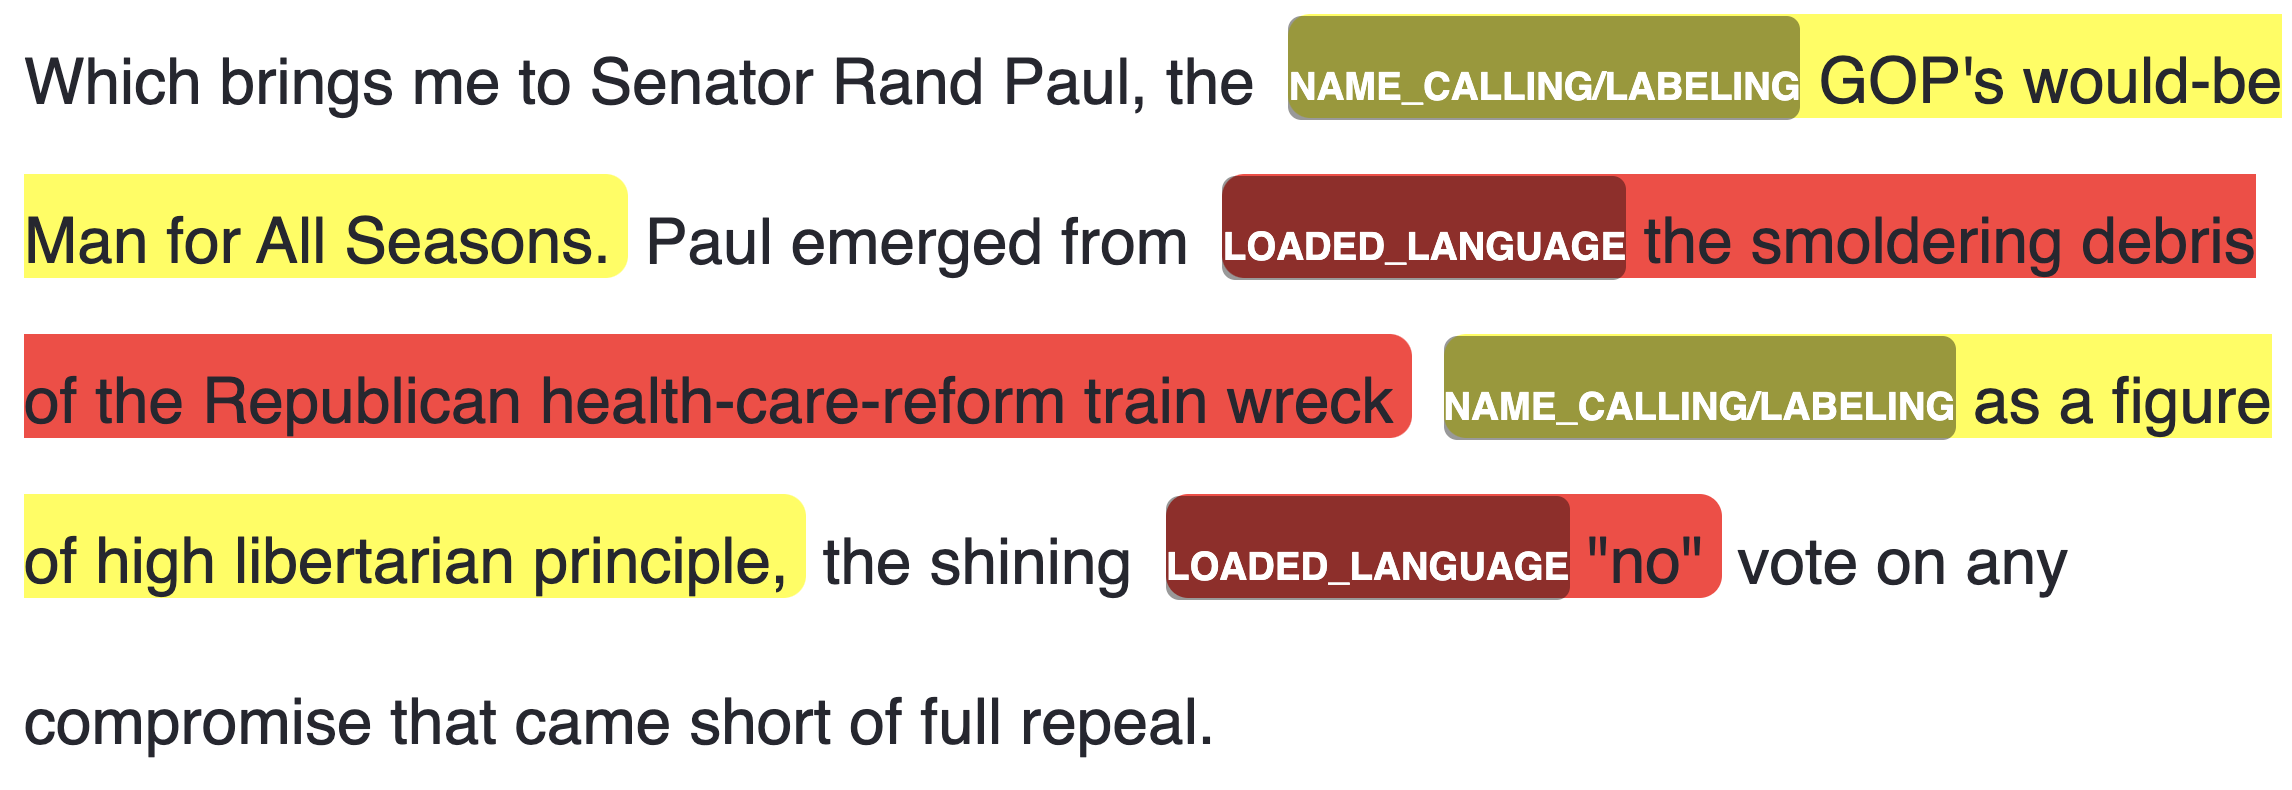
\includegraphics[width=\linewidth]{figures/propaganda_example_1_color.png}
    \caption{Detection of propaganda techniques using~\citet{baly2020we}.% the article comes from NationalReview, a source with Right-leaning bias.
    }
    \label{fig:propaganda_example_1}
\end{figure}


%For the propaganda analysis, we are focusing on the computational propaganda, defined as the propaganda that has been analysed by computational approaches. 
%The survey conducted by~\citet{da2020survey} displays the most important works, and also underlines the main limitation of current methods.
%The biggest limitation that we see, is that \emph{explainability is a desirable feature} but current approaches do not provide it.
%Most of the models only classify full articles as being propagandist or not~\cite{barron2019proppy,rashkin2017truth}, and this does not help to understand why.
%Therefore, another work focuses on fine-grained techniques~\cite{da2019fine}: every article analysed is annotated with labels coming from 18 different techniques, also indicating the spans affected by the techniques. So we can see where propaganda is inside an article and which specific techniques were used. Figure~\ref{fig:propaganda_example_1}

TODO: The datasets for detection: article-level, fine-grained

\subsection{\statusred Limitations}
HERE?

\subsection{\statusgreen Layers of information}
\label{ssec:lit_layers_of_info}
We see this as text conveying two layers of information:
\begin{enumerate}
    \item the first layer, the most visible, is the layer of \emph{facts}: entities (what/who is mentioned) and actions (what happens), combined into events
    \item a second layer of additional and subjective information: choice of terms to use, details to include and exclude, order of presentation, expression of opinion, subjective statements. All these means are used to convey a certain point of view, and therefore we use the umbrella term of \emph{persuasion}.
\end{enumerate}


% Talk here about different layers: 1 facts, 2 persuasion ( propaganda/argumentation/sentiment). Or in other terms: topical and non-topical elements.

These two layers can be more or less intertwined, and it can become more difficult to distinguish between them.
In the easiest cases, they can be identified on the linguistic surface of different words: some words in a sentence that belong to the \emph{facts} layer (e.g., a name) accompanied by other words that belong to the \emph{persuasion} layer (e.g., an adjective).
In this case, it is conceptually easy to separate the two components in a text and say which word belongs to one or the other.

But in many other cases, the two components can also coexist within the same word. For example, a term may have been chosen both to communicate a certain concept (facts layer), but between many available terms, the author voluntarily or involuntarily picks one or another term that conveys a different opinion on the concept itself (persuasion layer).

% e.g. name+adjective, where the name is the topical element while the adjective can express the opinion of the writer (commenting, denigrating, complimenting, subjective).
% Or they can also be expressed in the same word together: this is where word selection applies. For example, when the writer needs to find a word for communicating a certain concept ``?", they can choose whether to use X or Y. While these two words have the same underlying concept, they express it quite differently.

% Or also called: Topic model and Anti-topic model (expand on this, as discussed during the upgrade)

% Propaganda: Communication with the goal to persuade

Our hypothesis is that \emph{we can distinguish between the two layers}.

We will discuss this hypothesis in Chapter~\ref{chap:linguistic_persuasion}


\section{\statusred Political Leaning}
\label{sec:lit_leaning}

\todo{Continue here to take all citations from Chapters 5-6 and expand on them}

Here in this section, we focus on the concept of Political Leaning.

First, we give a definition, and then we focus on the Political Leaning Classification task and how it has been addressed by the literature.

\subsection{Political Leaning Definition}

Political Leaning is a term that is derived from Political Ideology~\citep{jost2009political}.
Political ideology is defined as a ``set of beliefs about the proper order of society and how it can be achieved"~\citep[p.~64]{erikson2015american}.

From the multi-dimensional diversities in political ideologies, there is a historical tendency to consider only the Left-Right dimension~\citep{jost2009political}.
Although this simplification does not capture completely the complexity of determining one's political ideology, it is the most common way of describing political orientation.
Since only one dimension is considered, it is usually named as a political leaning or political spectrum.

% historical left and right

% https://www.dictionary.com/e/politics/political-spectrum/
% https://en.wikipedia.org/wiki/Political_spectrum
Historically, the usage of left and right originate during the 1789 French Revolution. The physical position of the politicians in the French National Assembly was that the revolutionaries were sitting together on the left side, while the aristocracy-favouring was on the right.\footnote{\url{https://www.dictionary.com/e/politics/political-spectrum/}}
Therefore, the newspapers started using the terms to mention respectively the liberal (left) and the authoritarian on the right.

From originally only two labels, in 1857 we have the first appearance (on the Southern Trade magazine) of the term \emph{political spectrum} to describe the range of political opinions.


% US and conservative vs liberal
% https://pleeps.org/en/wp-content/uploads/Political-Ideology-Its-Structure-Functions-and-Elective-Affinities.pdf (jost2009political)
The use of ``liberal" and ``conservative" as substitutes for ``left" and ``right" is becoming more prevalent in the United States and other countries.
This terminology effectively captures the historical ideological division between desires for change and stability.
These two desires, change vs maintaining the status-quo, are coming from debates that have their roots in age-old disputes regarding the appropriate levels of hierarchy, authority, and inequality~\citep{bobbio1996left}.


% https://pleeps.org/en/wp-content/uploads/Political-Ideology-Its-Structure-Functions-and-Elective-Affinities.pdf (jost2009political)
This formulation of the distinction between left and right is characterised by
two different aspects~\citep{jost2018political}:
\begin{itemize}
    \item supporting vs opposing social change
    \item rejecting vs accepting inequality
\end{itemize}
The most common terms that people from both left and right associate with the right are: “conservative,” “system maintenance,” “order,” “individualism,” “capitalism,” “nationalism,” and “fascism,” and they associated the left with “progressive,” “system change,” “equality,” “solidarity,” “protest,” “opposition,” “radical,” “socialism,” and “communism”~\citep[p.~213-14]{fuchs1990}.
The two core components of the left-right dimension, attitudes towards change versus stability, and equality versus inequality, are connected due to historical factors, as Western societies have gradually become more egalitarian over the past few centuries in terms of human rights and liberties, economic distribution, and political power distribution.
Equality has increased in some instances due to revolutionary events, which were frequently resisted or opposed by conservatives and those associated with the right~\citep{nosek2009politics,burke1790reflections}.



% automated paragraphs
Left-leaning ideologies are typically associated with progressive and socialist ideas, such as the belief in social equality, the importance of government intervention in economic matters, and the provision of public services.
Right-leaning ideologies, on the other hand, tend to prioritize individualism, capitalism, and free markets, with less emphasis on government intervention and regulation.

However, the specific meaning of left and right can vary across countries and political systems.
For instance, in some countries, left-wing political parties may advocate for more social welfare programs and nationalized industries, while in others, they may focus on issues such as civil liberties and human rights.
Similarly, right-wing parties may prioritize issues such as nationalism, religious conservatism, or economic liberalism, depending on the country's culture and political history.

Furthermore, the labels ``left" and ``right" can also be influenced by the particular issues and events of a given time period.
For example, in some countries, environmentalism and climate change have become important political issues that may cut across traditional left-right divides.
Similarly, issues such as immigration, trade, and national security may be more salient in certain countries than in others, shaping the way that people identify with different political ideologies.




% practical definition: view on issues
As a more practical and operable definition, we can define political leaning from the common positions that left and right have on issues such as economics, social policies, and governance.

% Position of the left and right (wikipedia/allSides):

% https://www.allsides.com/media-bias/rate-your-bias
\begin{table}[ht]
    \centering
    \begin{tabular}{p{0.2\linewidth} | p{0.4\linewidth} | p{0.4\linewidth}}
      Topic  & Left & Right \\ \hline
      Social issues & \\
      Abortion & rights of the mother, ability to have abortion & rights of the fetus, limiting and stopping abortions \\
      Gay marriages & no difference with opposite-sex couples & marriage between man and woman, gay marriage is different from what God intended \\
      Family & expanded view on non-traditional families & not encouraging divorced/single/unmarried parents (accepting them may be fine) \\
      Sexual and Gendered behaviour & accepting and empathetic culture & \\
      Sexuality & free expression is a right & \\
      TODO finish
    \end{tabular}
    \caption{Left and Right positions according to AllSides}
    \label{tab:allsides_leaning_positions}
\end{table}

Table~\ref{tab:allsides_leaning_positions} shows how AllSides recaps the common positions about different issues.\footnote{\url{https://www.allsides.com/media-bias/rate-your-bias}}.




\subsection{Political Leaning Classification}
\label{ssec:lit_leaning_classification}

FROM TTO2020

%First we present literature on political leaning prediction, then on propaganda detection, and how the two analyses could be connected. %with the possible points of contact and why the two analysis could benefit from an integration.

%\subsection{Political Leaning}
% Political leaning classification

Political leaning detection models have been produced for general media sources~\citep{budak} or for 
specific political corpora such as congressional records~\citep{gentzkow}, political party websites~\citep{yan2017perils}, and political blogs~\citep{ahmed201}.  
Others focused on inferring the political leaning of Twitter accounts~\citep{Cohen2013ClassifyingPO}, Facebook users~\citep{Bakshy1130}, politicians~\citep{thomas-etal-2006-get}, or political writers~\citep{iyyer-etal-2014-political}. 
Various analysis methods were used in such studies, such as linguistic analysis \citep{gentzkow}, graph analysis \citep{chen2017opinion}, topic modelling \citep{ahmed201, Cohen2013ClassifyingPO}, support vector machines (SVM) \citep{Bakshy1130,thomas-etal-2006-get}, and neural networks \citep{iyyer-etal-2014-political,baly2020we}. In this paper, we focus on detecting political learning of articles in a corpus of general news from a wide variety of sources (see Section~\ref{sec:dataset}), using a neural network approach fused with propaganda features. %\todo{description ok?} 

%often used supervised or unsupervised models applied to , or on opinion graph mining ~\cite{thomas-etal-2006-get}.

%gentzkow - linguistic analysis 
%yan2017perils - regression models and neural networks
%budak - supervised learning and crowdsourcing
%ahmed - topic models
%Cohen2013ClassifyingPO - SVM and topic models
%bakshy support vector machine 
%thomas - svm
%iyyer - NN
%chen - SVM, LDA

%Most models use supervised or unsupervised machine learning algorithms, trained using source annotations or crowdsourced articles annotations  
 
%underlined that most of the approaches do not generalise well across domains. 
%As~\citet{yan2017perils} underline, three different classifiers trained on different types of texts (domains: congressional records~\cite{gentzkow}, political websites, wiki) result in lack of cross-domain generalisability (classifier trained on different domain struggles to find correct label on another domain, and mixing the training data reduces performance confusing the models).

In~\citet{baly2020we}, authors used a BERT-based model for predicting the political leaning of individual articles. The model takes as input the text of the article and produces one of three labels: Left/Centre/Right. The model is trained with a corpus from AllSides website\footnote{\url{https://www.allsides.com}} which groups articles %with their political leaning 
according to the leaning of their source or of their author. %\todo{manually?}
%Authors found that 3.11\% of their 34737 articles from AllSides has a different leaning to that given to their sources (AllSides confirmed that this is due to using author-based leaning). 
%   \item source-level annotation: in most of the cases, the articles are annotated with the bias of the media outlet
 %   \item author-level annotation: sometimes, the articles are annotated with the bias of the specific writer, which can be
 % Similarly to \citet{baly2020we}, in this paper we also focus on classifying articles, regardless of their source and authorship. However, %unlike ~\cite{baly2020we}, 
 % unlike previous work, we use propaganda features in the political learning prediction model.   

% - Problem: learning the source instead of the political leaning
%Main focus in~\citet{baly2020we} is to classify individual articles regardless of the source or author. This generalises better with unseen sources, and with cases were there is a difference between the political leaning of a particular article from that of its source. Authors found that 3.11\% of their 34737 articles from AllSides has a different leaning to the given to their sources (AllSides confirmed that this is due to using author-based leaning labels for some articles). 


%Other approaches focus on learning the media bias of a the source~\cite{baly2020written,biessmann2016automating}.
%This is based on the observation that in their dataset (collected from AllSides) there are some articles (1,080 individual articles, 3.11\% on a total of 34737) having a leaning different from their source leaning.

%To clarify this point, we personally asked to the AllSides team about this discrepancy between article-level bias and source bias, and we understood that there are two types of annotation:
%\begin{itemize}
 %   \item source-level annotation: in most of the cases, the articles are annotated with the bias of the media outlet
 %   \item author-level annotation: sometimes, the articles are annotated with the bias of the specific writer, which can be different from the media bias\footnote{\url{https://www.allsides.com/media-bias/media-bias-ratings\#ratings}}
%\end{itemize}

%Therefore the 3.11\% is due to the author-level annotation. We want to underline that in this way, the annotation of the political leaning is not specifically assigned to the single article but instead it is assigned to the author. It is still a "distant supervision" in some extent.

% - Problem: domain generalisation does not work
%Other works on political orientation prediction underlined that most of the approaches do not generalise well across domains. As~\citet{yan2017perils} underline, three different classifiers trained on different types of texts (domains: congressional records, media websites, wiki) result in lack of cross-domain generalisability (classifier trained on different domain struggles to find correct label on another domain, and mixing the training data reduces performance confusing the models).


% TODO: Is this really a consequence of the previous paragraph?
%Because of this lack of generalisability, 
%Other models focused on identifying political leaning using opinion graphs that represent how (positive/neutral/negative) the political leaning sees a set of extracted entities~\cite{chen2017opinion}. The prediction of the classifier, after extracting the entities in the text, compares the orientation towards the entities and picks the most similar side.
%The task of topical stance is also explored in other works in relationship to the political leaning of a whole news source~\cite{stefanov2020predicting}.
%A similar approach is described in~\citet{jiang2008political}, where instead of opinion the term used is subjectivities. The authors show how, by using the same model (Bag of Words) on the subjective sentences only, it is actually easier to classify political leaning. Furthermore, they mine Opinion Expressions which represent the orientation towards specific expressions (e.g., the liberal political leaning usually refers to ``democratic party'' using a positive subjectivity).
%These models rely on the fact that political leanings often have a stable view on some topics\footnote{\url{https://en.wikipedia.org/wiki/Right-wing_politics}}\footnote{\url{https://en.wikipedia.org/wiki/Left-wing_politics}}.








% Sentiment analysis

% Propaganda analysis

% Fine-grained

% AllSides and comparison of multiple sides, the summary contains some insights about the biggest differences between the political sides.

% Bias / political leaning classifier:
% - baly et al 2020: just based on text
% - we could help the models focusing on the layer of presentation/bias/propaganda instead of having the full text



% Two axes:
% - common/unique
% - objective/subjective/framing

% Different. The first one can be observed with similarity analysis. The second one with sentiment/propaganda/framing analysis.

% The left/center/right political leaning is mostly positioned on the common/unique axis.

% Hypothesis: the two axes are very much correlated. Looking at the framing axis can help to distinguish political bias.

% We try in the next sections to see if this is true.



\section{\statusred Topics}
\label{sec:lit_topics}

\subsection{Topic definition}
\label{sec:lit_topics_def}

What it is:
- categories / groups 

How it relates to concepts described in this thesis:
- headlines, clusters
- topic and anti-topic layers/words: refer to Chapter~\ref{ssec:lit_layers_of_info}

\subsection{Computational Approaches}
\label{sec:lit_topics_computation}


Explain here different tools/methods that provide topics/entities

We have approaches that try to determine the topics without having external knowledge, and approaches that instead an existing taxonomy/list of topics and try to map the input documents to them.

\subsubsection{LDA topics}

One of the most common methods to extract topics is to ``automatically detecting them" from the corpus.
The idea is to learn from the data and by selecting a specific number of output topics, we get them.
Problem: difficult to extract labels

The problem of assigning labels: can we really tell what is different about the groups?
Need to know beforehand how many topics we want in output.
TODO

Topic identification is a method for identifying hidden subjects in enormous amounts of text1. It can help you find common themes or keywords that represent the main ideas of a document or a collection of documents. For example, if you have a set of news articles, you can use topic identification to find out what are the most discussed topics among them.

One of the techniques for topic identification is called Latent Dirichlet Allocation (LDA)12. It is a statistical model that assumes that each document is composed of a mixture of topics, and each topic is composed of a distribution of words. LDA can learn these topics and words from the data without any prior knowledge or labels. LDA can be implemented using Python’s Gensim package1, which provides various tools for natural language processing.

LDA is a type of topic modeling that uses a latent Dirichlet allocation approach12. Topic modeling is a form of unsupervised learning that can be used for exploring unstructured text data by inferring the relationships that exist between the words in a set of documents23.

LDA assumes that each document is composed of a mixture of topics, and each topic is composed of a distribution of words13. LDA can discover topics that are hidden (latent) in a set of text documents by inferring possible topics based on the words in the documents34. LDA uses a generative probabilistic model and Dirichlet distributions to achieve this4.

Another technique for topic identification is called bag-of-words2. It is a simple way to represent text data as a collection of words and their frequencies. Bag-of-words ignores the order and structure of sentences, but it can capture some basic information about the content and vocabulary of a document. Bag-of-words can be used with simple NLP models such as TF-IDF or Naive Bayes to identify topics from texts.


\subsubsection{Entity Annotators}
DBPedia spotlight: entity annotation is not very good. It struggles to recognise all the entities in the articles (proof?) → DISCARDED
BLINK (Facebook): huge (30GB models to fit on RAM), not running on my laptop. On server: no NVIDIA drivers (wants GPU) → DISCARDED
Spacy-entity-linker https://github.com/egerber/spaCy-entity-linker/ . Not very widely used. → DISCARDED

Then from entities, need ways to derive the topics by navigating knowledge bases (wikidata in most cases)

\subsubsection{TextRazor}
TextRazor: seems more accurate, industrial, FreeBase taxonomy. Each entity is annotated with wikidata id and a list of FreeBase types. Also provides topics and fine-grained topics

benchmarks? check that it is better than other tools
% Regarding the validation of TextRazor, I am not aware of a benchmark done to check if it is better than other tools. It was suggested by Harith to use it, and I find that the data it provides is generally quite good (for topics and entities). But this is qualitative, I didn’t do a benchmark or looked up for benchmarks. The assumption was that it’s a commercial product and it should be good.
some papers that claim to do benchmarks:
http://giusepperizzo.github.io/publications/Rizzo\_Erp-LREC2014.pdf for the entities
https://www.linkedin.com/pulse/google-nli-kill-market-linguistic-apis-review-yuri-kitin/ mentioning that TextRazor is useful because it links to Wikipedia/DBPedia

TextRazor is the only one that provides already hierarchical topics, the other ones always give topics that are not hierarchical or can be made hierarchical with external knowledge (e.g. using DBPedia to navigate broader topics).

What it provides


\section{\statusred Other related phenomena}
\label{sec:lit_related}

TODO: here talk about misinformation, argumentation mining and defend the scope of this thesis: propaganda.

But at the same time mention the relationship with them

\subsection{Propaganda and Misinformation}
\label{sec:lit_related_misinformation}

Work of~\citet{orrumachine} where persuasiveness is observed to exist more in fake news outlets: discursive repertoires that are more persuasive appear more in fake, while some other discursive repertoires that are less persuasive appear in more trustworthy news outlets.




\cite{roozenbeek2022countering} Good evidence that making people aware is helpful, people can learn to recognise manipulation techniques (it worked on YouTube). The paper talks about manipulation, but the techniques overlap with propaganda and logical fallacies. Also shifts the goal from recognising True/False to recognising manipulation. Work from Psychology.

Cite TTO2019 comparison of different credibility measures, and we saw that propagandistic sources are usually considered as part of misinformation (MBFC dataset that usually places propaganda inside ``questionable news sources" = ``fake news").


\cite{romain2022misinformation} persuasive writing strategies for misinformation detection (TODO analyse this paper)

\subsubsection{Rating news sources in different aspects}

TODO: here talk about all the tools/websites that rank news sources or score them with respect to misinformation/propaganda/bias/leaning

\subsection{Propaganda and Populism}
\label{sec:lit_related_populism}

Relationship between propaganda and populism:
~\cite{oates2021rewired,tumber2021routledge,pasquino2008populism}
%https://ebrary.net/177441/sociology/the_routledge_companion_to_media_disinformation_and_populism
they are very strictly linked.
% http://www.ask-force.org/web/Fundamentalists/Pasquino-Populism-and-Democrady-2005.pdf 

In~\citet{oates2021rewired}, ``rewired propaganda"
concept of ``rewired propaganda" that analyses the interplay of propaganda and populism in the digital age. In particular, an awareness of the classic concept of propaganda allows us to see how the democratising effect of online information to create informed citizens is outmatched by the internet’s ability to leverage misinformation in the service of populist propaganda.
In other words, propaganda can now ‘hide in plain sight’ as it is so difficult to disentangle from the broad range of information in the digital sphere.
The concept of ‘rewired propaganda’ is suggested as way of understanding a communicative method that leverages misinformation, campaign tactics, and the way both traditional and social media functioned in the 2016 US elections.
``When populism replaces party-based politics rooted in ideology and articulated policies, rewired propaganda becomes as powerful in democracies as it has been in non-free states such as Russia."

% another concept from the literature that is shown to be close to persuasion and propaganda: \gls{populism}~\citep{tumber2021routledge,pasquino2008populism}.\todoHA{Not mentioned in intro. Why not?}
% We want to understand: what is the substantial difference between populism and propaganda? Can these two phenomena be related?
% This question arises purely from a logistical point of view: we have automated methods for detecting propaganda, but we do not have tools to detect populism. Therefore, if we can prove that populism and propaganda are actually correlated, then it becomes not important for us to be able to detect something that is very much correlated to something else that we already detect.

% % concepts
On the conceptual level, propaganda and populism are two distinct concepts. The first describes more the persuasion mean used to push for an agenda, while the second one is usually used more together with the actor that wants to push the agenda. Populism is ``a type of politics that claims to represent the opinions and wishes of ordinary people".\footnote{\url{https://www.oxfordlearnersdictionaries.com/definition/english/populism}}
And to be on the side of ordinary people, it uses propaganda as a mean. So a populistic \emph{actor} uses propaganda \emph{techniques}. Conceptually, they are related.
% We need them to be related to demonstrate that propaganda exists across all political leanings.


Literature shows “populism” as a concept together with Propaganda
What is the difference between populism and propaganda?
% Can we use some datasets about populism to understand how they contain propaganda?

% Dataset found: populism in political speeches %https://dataverse.harvard.edu/dataset.xhtml?persistentId=doi:10.7910/DVN/LFTQEZ&version=2.0 
% Each annotator (4 for each speech) gave a score between 0 (non-populistic) to 2 (very populistic)
% 4961 rows 
% 1240 deduped (352 left, 256 center, 469 right, 652 NA)
% Languages: 265 en (304 es, 148 pt, …),
% Leaning of the english ones: (36 left, 37 center, 84 right, 106 NA)

TODO: take from Chapter 5 some description of populism across political spectrum

We will use the concept and literature of \gls{populism} in Chapter~\ref{ssec:ps_prop_leaning_imbalanced} to analyse the imbalance of propaganda datasets.


\subsection{Opinion and Subjectivity and Manipulation?}


\section{\statusred Discussion}
\label{sec:lit_discussion}

Limitation of literature: fragmented and not considering everything together.

Theoretical works (TODO examples) consider propaganda in different situations (e.g., one nation/context for each paper), but missing a comparative analysis across leanings.



Consequence: limitation 2:

Existing propaganda datasets may be unbalanced, as it is not completely clear how they select a set of sources. By using external dimensions we may discover that there is imbalance.

\section{\statusred Scope of this work}
\label{sec:lit_scope}

Main ingredients:

- Propaganda detection

- Political leaning

We see that the two can be related and we want to understand their relationships.
How does propaganda change across political leaning?
Can we recognise the political orientation of a piece of news from how it uses propaganda techniques?
How does propaganda relate to shared/unique information? How do small variations relate to propaganda?

What is outside scope?
Developing/refining deep learning models to recognise propaganda techniques. We want to combine existing models and use a combination of features.


\chapter{\statusgreen Common Ground Search}
\label{chap:common_ground_search}

% \todoAWinline{The point of reproducing the expt. is to determine how well their technique supports your own research aims. So this section really wants to have some quantification of the results. But also, you're interested in the qualitative question of how well you can identify those sentences which are not the basic statements of fact. So you want this chapter to lead into a discussion of how well you can identify the factual v. manipulative sentences, and the degree to which the non-factual sentences can be used to identify propaganda etc.}
% \todoHA{I agree}

% \todoHAinline{Overall, I can see a good chapter here, but need a good revision to better link the experiment with the RQs in this thesis, to detail the data used, detail the results and explain them more thoroughly, to describe the steps and rationale of the experiments more clearly (structure). And to more clearly explain the contribution beyond just replicating a previous paper.}

\section{\statusgreen Introduction}

% TODO: Research Question of this chapter
% Summary of findings / contributions
% - limitations of current methods for corroboration/omission detection
% - similarity methods ? 
% - 

% chapter motivation: multiple versions of the same story 
% This chapter contains the first set of practical experiments that we carried out.
% \todoHA{Run Grammarly on all text}
% general goal
This chapter aims to analyse how different articles present the same event from different perspectives.
For each \gls{event}, different news sources publish a big multitude of articles.
These articles can be more or less similar between them, possibly leading to a variety of linguistic forms. %\todoHA{Articles about same events does not necessarily mean you get a variety of linguistic form} 
Therefore, this is an excellent opportunity to study the relationship between the bare facts (common ground) and the additional choices that are made to try to persuade the reader of a specific opinion (as discussed in Section~\ref{ssec:lit_layers_of_info}). % (with phenomena such as framing, interpretation, manipulation, propaganda).\todoAW{How similar are these terms? Framing is much less loaded than Propaganda}\todoHA{Only mention the ones you are studying}

% fit into thesis
% But how does this fit into the overall goal of the thesis? Our overall research questions aim at studying the relationship between propaganda and political leaning (overall \acrshort{rq}1: \textbf{What is the relationship between propaganda and political leaning?}).\todoHA{Unclear how this chapter is connected to this RQ}\todomargin{general goal, and RQ1 is specific: To what extent do news articles about the same events differ?}
% But, first of all, we need to take awareness that 
% In order to study persuasion techniques as the additional layer on top of the facts (as discussed in Section~\ref{ssec:lit_layers_of_info}) we want to exploit the multitude of writings about the same topics. 
For this reason, this first experimental chapter is about parallel news and comparing the shared information between the articles.
% Given that the articles are a mix between raw facts and this additional layer of persuasion, %/opinion/propaganda,\todoAW{Interesting that you didn't include "framing" here...} % framing not used because it is more difficult to detect agenda setting (e.g. selecting what to include in article? But at the same time this chapter is about omission and corroboration so should be related
Considering articles coming from different news sources, that have potentially different political ideologies, we aim to extract which parts are shared and which parts are instead unique to each article.
% which part is shared and therefore is likely to be more closely related to the base layer of facts.\todoHA{?}
Relying on this analysis, we may understand the point of view of each article and how it differs from others.
%(TODO: to retake this afterwards and talk about credibility signals from bountouridis corroboration omission).
% Having this first differentiation between shared, omitted and unique, we also want to assess whether this is correlated to language that wants to persuade (propaganda). --> chapter 4 

Our experiments, therefore, are directed at automatically comparing and finding differences in similar articles, and trying to understand the reasons for articles to be different or similar.
%\todoHA{How does this fit with your RQ?}

% RQ of this chapter
For this reason, we dive into the work of spotting similarities and differences between multiple articles.
Our Research Question for this chapter is \acrshort{rq}1: \emph{To what extent do news articles about the same events differ?}
We divide it in several sub-questions: 
\begin{enumerate}[label={\textbf{RQ1.\arabic*:}},leftmargin=2cm]
    \item How are new events reported differently by multiple sources?
    \item How could we identify what is unique for each report and what is common? 
    \item To what extent can we automatically detect omission and corroboration across multiple articles?
    \item Which similarity metrics are best for detecting omission and corroboration?
    % \item What type of document/sentence encoding performs better to detect corroborations and omissions? OR What are the characteristics that allow encoding better documents and sentences?\todoAW{Is this a technical question? (ie. what's the best parser, for example?) "How can we automatically detect...?" and then expand in the main body of the text}
    % Is there a link between the parts that are different and propaganda/loaded language? --> chapter 4
\end{enumerate}



% find the shared information across several articles, and identify which parts are changed/unique. How sentences are changed between multiple articles.
% We take from the work of~\cite{bountouridis} and expand ...

% overview of subsections
In the following sections, we first give an overview of the data resources available for this task (Section~\ref{sec:cgs_data}). Next, we
analyse in Section~\ref{sec:cgs_cross_referencing} an existing approach to detect corroborations and omissions between articles. Then in Section~\ref{sec:cgs_similarity} we explore the methods to compute document similarity, and in Section~\ref{sec:cgs_clustering_and_differences} we describe our method to extract fine-grained differences at the word-level. Finally, in Section~\ref{sec:cgs_findings} we discuss our findings.

% % method
% Method: 
% hierarchical clustering of sentences, omissions/corroborations + changed parts
% Ranking of similarity by models and by me


% Findings?
% threshold of similarity challenging to find. Meaning and sentence similarity don’t always go together (all models tried)


% Limitations?



% Outline

% - cross-referencing articles (bountouridis)
% - similarity
% - sentence clustering and small differences





% \section{from upgrade report (TODO)}

% During the first year, several activities have been done.
% Some have been done as initial explorations in the field of research, understanding what other researchers have done, ``getting the hands dirty'' with data and NLP tools.
% And their function within the PhD project has been to lead to the Research Questions that we described earlier.
% Some other activities have been done to kick start the future experimentation, for example doing data collection of news articles or by beginning to implement some of the stages of the processing pipeline that will be used.
% % , with the goal to find and formulate proper Research Questions and to prepare the execution of the proposal.


\section{\statusgreen Data Resources}
\label{sec:cgs_data}
% what
% We also started collecting, early this year, several types of data that will be useful for the analysis planned.
% For this first chapter, we have been focusing on parallel news dataset. We started by using existing datasets, and then we started collecting on our own because we wanted specific features.
To analyse parallel news, we consider here both existing datasets, ready to be used, and also resources that we collected from scraping the public web.
% why
% The reason for this, is that 
We are interested in specific features, and existing datasets are not always having all the requirements.
First of all, a wide set of articles is needed, dense in time and from a wide variety of news outlets. We need substantial overlap between articles and the more sources we can include, the better we can observe variations of the framing phenomena.
Another very important feature is to have a good pre-clustered set of articles to help the curation of a dataset, %especially for the first Research Question, 
by knowing that the articles are well-related.
% Then, when we will have the document clustering in action, this feature is not anymore required, but still can serve as a benchmark for that stage.
If we substitute this requirement with a clustering algorithm, we need to ensure a high quality of the clusters. We decided instead to use articles that are already grouped together, to remove an additional source of issues.
A last desirable feature would be to have articles that come from sources with different opinions, such as different political ideologies. %, that would be beneficial to create examples especially for the user study, where we want to maximise the occurrence of framing techniques. 
This is because the general goal of this thesis is to study persuasion and propaganda, so if the points of view are different we can see the propaganda more easily.

% how
% - google news (more than 500k articles) daily. Some stats about the number of sources involved  TODO: how is it made? What are its properties? Why useful?
Given these requirements and after exploring different news aggregators, we found that Google Headlines Full Coverage feature\footnote{\url{https://www.blog.google/products/news/new-google-news-ai-meets-human-intelligence/}} would fit the requirements of covering a big number of news sources (the \texttt{en-GB} version contains articles from more than 10k domains) and being very dense (an average of 9k new articles each day).
The data comes divided by topics (Latest, United Kingdom, World, Business, Technology, Entertainment, Sports, Science, Health) and inside each topic, the articles are grouped into ``stories''. Each story has articles from the most relevant sources (``Top coverage'') and then also lists articles from other less important sources, for an average of 40 articles per story.
The stories are created automatically by Google News, and this makes available an enormous number of articles and sources updated continuously. %it to be always updated and be diverse in the sources included.
We captured every day, during the March–September period of 2020, the published set of stories. In this way, we managed to retrieve more than 700k articles. Not all the articles listed can be retrieved because of paywalls or other blocks by the publishers.

% - allsides: human-created with interesting framing differences
Another data source that we actively retrieve is AllSides which provides a curated set of ``headlines''\footnote{\url{https://www.allsides.com/story/admin}} where three articles with different political alignments are put together and compared in their difference.
The curators describe how the story gets framed by the considered sources, using natural language.
This description usually contains the usage of terms or themes that get mentioned.
%At the end of June, we have available 4764 headlines, with 13979 articles linked.
Differently from Google Headlines which has different versions for each country, this data is US-focused being curated in the US and therefore has a much more limited scope. Also, the discussion of bias and framing is mainly focused on political issues, while other data sources (such as Google News) are more general. %we want to focus also on other types of differences of opinion.
% role of this specific data
% This data, although the description of the differences is not directly parsable, will be used to feed the user study and understand the role of comparing different sides.

% - allnews: standard benchmark, wide adopted (find refs)

% scraping is legal for research: https://aballatore.space/2020/04/01/web-scraping-is-legal/

% % role of this
% The data collection done in these current months will continue across the PhD, and will be used in different stages of the analysis. It will serve as the seed to create the labelled dataset for the first Research Question and also provide a wide set of articles from different news sources to empower the studies of the second Research Question.
% Having articles from so many different news sources, we can on one side provide some indication of framing for news sources that are not usually targeted by manual framing studies because not enough ``important'', and on the other side be more confident to observe some phenomenon of information re-usage that is the underlying hypothesis for the last sub-question.
These two data sources are used for this and the next chapter. From Chapter~\ref{chap:political_sides} onward instead we rely mainly on an existing dataset, still coming from AllSides~\citep{baly2020we} because we want to compare our results with other works.

In this chapter, we also use \emph{All-the-news}\footnote{\url{https://www.kaggle.com/datasets/snapcrack/all-the-news}} which includes more than 140k articles published by fifteen major US outlets.
The articles are collected by using RSS feeds or collecting directly from the homepages of the news sources. The sources in question are: Atlantic, Breitbart, Business Insider, Buzzfeed News, CNN, Fox News, Guardian, National Review, New York Post, New York Times, NPR, Reuters, Talking Points Memo, Vox and Washington Post.
The articles are not balanced across news sources, as some sources were more prolific than others in the considered period.
The topics of the news are not limited to anything specific, and therefore the news articles include very different topics.


\section{\statusgreen Corroboration and Omission Extraction}
\label{sec:cgs_cross_referencing}
% Experiment 1
% what
Articles may share information, so the first step for our analysis is to identify which parts are in common and which others change.
We started by taking as reference the paper from~\citet{bountouridis2018explaining} which presents a methodology to analyse how much information overlaps between different similar documents, identifying points of information that are \gls{corroborate}[d] or \gls{omit}[ted].

The main message of the paper is that sources that \gls{corroborate} the most are also sources that get a higher ``factual reporting'' score (as measured by Media Bias/Fact Check).\footnote{\url{https://mediabiasfactcheck.com/}}
Instead, the sources that \gls{omit} the most are the ones which get a lower score.
% why
% We wanted to analyse this resource because it seems to be going in the broad direction of our project, analysing different presentations in the news of the same event.

% details about this approach, be specific that is not my work. But thesis should be standalone
The approach used by the authors is the following:
\begin{enumerate}
    \item building document-level \gls{clique}[s]: documents are encoded (using TF-IDF), the matrix of their similarity is computed, then a threshold is applied to prune the similarity relationships. Afterwards, a graph is produced where the nodes are documents and the edges are the similarity relationships that satisfy the minimum threshold. This graph is then processed to identify the cliques and the outputs are then filtered to enforce that every document only belongs to one clique. Each clique represents a story that was covered by multiple documents (because they are similar between them). Not all the documents belong to a clique, they can be left out;
    \item building sentence-level \gls{clique}[s]: starting from the document-level cliques of the previous step (same story), each one of them is considered on its own, and the articles are split into sentences. Then, all the sentences are processed as in the previous step (encoding representation, similarity computation, similarity threshold, cliquing algorithm, clique post-processing). The outputs are sentence-level cliques that represent a piece of specific information that appears in multiple documents; 
    \item computing outlet-related corroboration and omission: sentence-level cliques are grouped by publishing outlet; then omitted cliques (appearing in other outlets but not in the considered one) and corroborated cliques (also appearing in other outlets) are counted;
    \item analysing correlation with factuality scores: the ratios of omitted cliques and corroborated cliques are compared with the scores coming from Media Bias/Fact Check for each outlet, and the hypothesis of correlation is verified: corroboration appears more in factual sources, while omission appears more in non-credible sources.
\end{enumerate}

% dataset
The dataset used is the \emph{All-the-news}\footnote{\url{https://www.kaggle.com/datasets/snapcrack/all-the-news}} which includes more than 140k articles published by fifteen major US outlets. To have the same results as the reference paper~\citep{bountouridis2018explaining}, we reproduce the paper by using only articles from 2016. This brings the analysis to work with 203 document-level cliques. 

% how
We analysed and reproduced this paper to get a deep understanding of how it works, and to extend its methodology to analyse the word-level differences. %\todoHA{Expand: anything else to be discovered?} 
The implementation started with the code and data %\todoAW{What are the properties of the dataset?} 
publicly provided by the authors,\footnote{\url{https://github.com/dbountouridis/InCredible}} but its incompleteness in some stages of the processing (e.g., the creation of the document-level cliques, and all the specific hyperparameters of the algorithms used) required integrating the codebase.\footnote{\url{https://github.com/MartinoMensio/InCredible}}

\begin{figure}[!htbp]
    \centering
    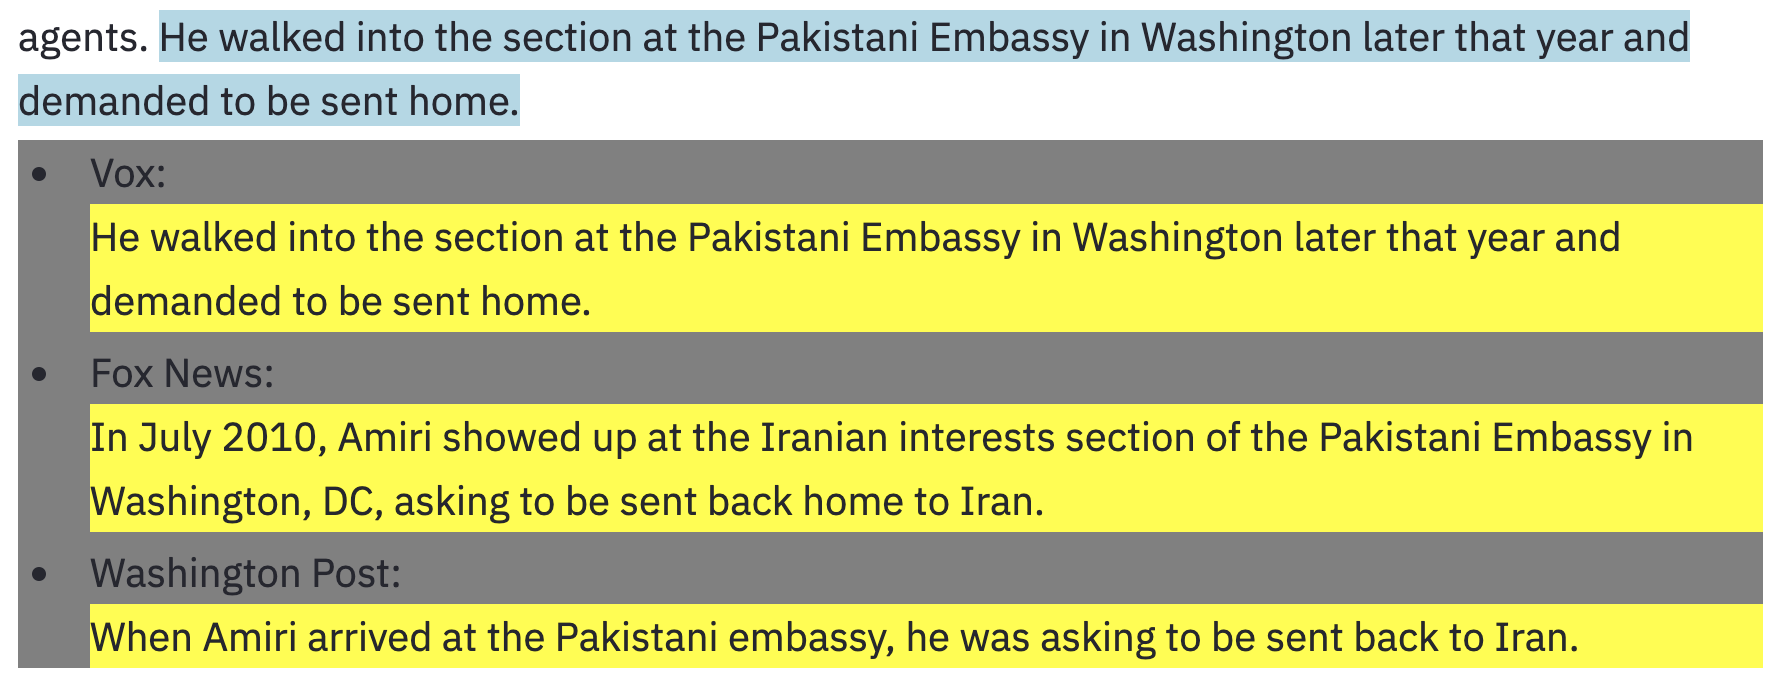
\includegraphics[width=\linewidth]{figures/cluster_similar_sentences_amiri.png}
    \caption{Corroboration example between Vox, Fox News and Washington Post.}
    \label{fig:cluster_similar_sentences_amiri}
\end{figure}%\todoHA{Good to have an example. But unclear what is the output, what did you get when processed these examples?}

An example of the reproduced analysis can be seen in Figure~\ref{fig:cluster_similar_sentences_amiri}.
In this example, the step 1 identified an article-level clique of 3 articles (Vox, Fox News, Washington Post) that cover the connection between Hillary Clinton's email and Amiri Shahram being executed.\footnote{\url{https://www.vox.com/2016/8/9/12410882/clinton-emails-trump-iranian-scientist-executed-amiri}}
The step 2 instead, identifies the three specific sentences that cover the detail of Amiri at the Pakistani Embassy in Washington.
Step 3 counts these sentences as corroboration between Vox, Fox News and Washington Post. 

\begin{figure}[!htbp]
    \centering
    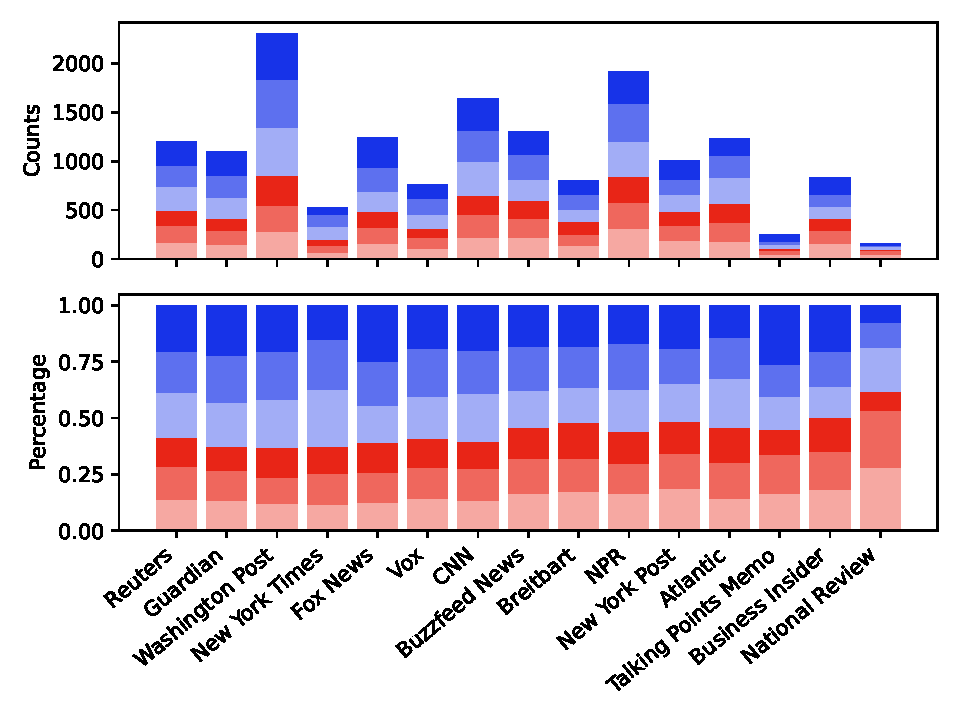
\includegraphics[width=\linewidth]{figures/bountouridis_fig_3_noGA.pdf}
    \caption{Corroborated (blue) and omitted (red) sentences per news outlet.}
    \label{fig:figure_3_bountouridis_reproduced}
\end{figure}%\todoHA{Do you point to this from anywhere?}

Figure~\ref{fig:figure_3_bountouridis_reproduced} shows our reproduction of the source-level corroboration and omission counts (top) and percentages (bottom).
Colour shading (quantised to three bins) indicates the average TF-IDF similarity among the sentences in cliques, i.e. the lighter the shade, the more dissimilar. This plot is almost identical to the one originally contained in~\citet{bountouridis2018explaining}, meaning that we reproduced correctly the complete approach.



% limitations
With the experiments and the interactive visualisation reproduced, we have been able to manually inspect the cliques of documents. For each of the 203 cliques of documents, we manually checked whether all the articles were topically related, and we observed that in 20\% of the cases, the document-level cliques were too wide (including articles from another main event) or too narrow (multiple cliques should have been merged together.
For a small portion (20 cliques), we inspected the sentence-level cliques to understand how similar the sentences were, and what types of differences they contained.
We identified the following limitations:
% and sentences identified by the model, seeing the following limitations:\todoHA{How? Method? How many? Give proper numbers}

\begin{itemize}
    % \item Their demo\footnote{\url{http://fairnews.ewi.tudelft.nl/InCredible/}} just shows one specific article as main and one specific clique (not very interesting)
    \item The \emph{document cliquing}
    %\todoAW{You've jumped very suddenly into the use of particular algorithms. What are these algorithms doing? How do you interpret their output? Are they your implementation or Bountouridis et al's? etc} 
    sometimes splits similar articles over different groups, or in some cases has different stories that talk about a different detail within the same clique (e.g., when a news story re-emerges because further details are discovered).
    This can be a consequence of having TF-IDF as the underlying method to represent the documents.
    This method is fast and efficient for coarse topic detection because, being based on bag-of-words, works well with specific terms that distinguish the topics.
    But when we need to have a finer-grained clustering such as in this case, the limitation of this method may surface: the terms of two political events with the same entities mentioned result in having similar feature vectors.
    It is not enough to change the thresholds to obtain better document cliques.
    \item The \emph{sentence cliquing} method provided just uses the degree of similarity between two sentences but does not point to which specific words are responsible for the similarities and differences. This would require a fine-grained analysis that in this paper is not included. Furthermore, sentences in a clique are very similar, and no significant differences have been observed because the similarity metrics are based again on TF-IDF. This method is not robust enough to the usage of synonyms and other variations on the linguistic surface, while at the same time is unable to distinguish two sentences that use the same words but have different meanings. These different meanings may be caused by the sentence structure or the role of the words. Therefore, selecting a threshold value becomes very difficult.
    \item The \emph{clique algorithms} are not the best choice for grouping when we have the information of how much similar two items are (a real-value instead of a binary-value is available from the similarity metric). The approach considers an unweighted version of the similarity graph by using a threshold (weights are just used to select the most appropriate clique during their creation). Instead, if we use the original weighted graph, we can use better and more flexible clustering techniques (e.g., agglomerative clustering). %, like agglomerative clustering
\end{itemize}
% \todoHA{All this is interesting but not very clear how you reached these conclusions and what they signify}





% In addition to these problems, the model described is based on TF-IDF which is not as robust with changes on the linguistic surface (as we saw in the next experiment).
% Models flourished
% This is the motivation for 5.1.2

% And also, it uses the similarity between TF-IDF just with a threshold, modelling the graph and cliques as unweighted (the weights are just used to select the most appropriate clique during their creation).

% role of this experiment
Reproducing this experiment helped us to see the limitations of this work. %, which belongs to the \emph{similarity} area of research (Section~\ref{sec:lit_relationships}).
This paper provides a great way to analyse the overlap between articles and extracts pieces that have been omitted or that are corroborated, but does not investigate further the reason behind the selection of what is included or not.
This opens up for further work:
\begin{enumerate}
    \item investigate how to represent the documents better to provide meaningful similarity metrics at the document and sentence level (Section~\ref{sec:cgs_similarity}); %\todoHA{Similarity of what? Why need it?}
    \item experiment with document and sentence clustering to bring up fine-grained differences. To understand the choice of terms, we first need to be able to identify how uniquely or commonly the terms are used across news articles that cover the same story(Section~\ref{sec:cgs_clustering_and_differences}); %e.g. how specific terms are chosen\todoHA{Where? Why?} (Section~\ref{sec:cgs_clustering_and_differences});
    % \item investigate the works that analyse framing theories and detection;
    \item investigate the reason for such differences to exist. This will be done in the next Chapter~\ref{chap:linguistic_persuasion} about detecting linguistic means of persuasion.
    % \item collect data from more recent articles that would be more relevant and interesting.
\end{enumerate}
% \emph{i)} , \emph{ii)} , \emph{iii)} , and \emph{iv)} g.

% Apart from these limitations, we are building our processing pipeline on top of this type of analysis, that links together news articles at different granularity levels (documents, sentences, words).
% This gives us the opportunity to use features from multiple articles for the next stage of automated detection of framing techniques.
This method of comparison has its main limitations in the similarity metric chosen. So we opted for doing some further research on the similarity metrics, in a way that accounts more for semantic similarity instead of just being term-based.


\section{\statusgreen Models for Similarity Analysis}
\label{sec:cgs_similarity}
% Experiment 2
% what
Since our biggest problem is representing documents and sentences in a way that captures more semantic similarity, we decided to analyse the existing works, including word embeddings and language models.
We wanted to see in practice how the usage of different representation models would affect the measurements of similarity, experimenting with a small set of articles. 
% finding and exploring more advanced methods to find the similarity between texts by using language models, we experimented on how to use these methods.

% why?
% is a pillar\todoHA{Too strong} for 
To compare different articles, we need to have a
solid base for computing the distances between them as a whole or more detailed to the sentence level.
The applications of similarity range from document clustering to the identification of omitted pieces of information in a cluster, therefore it is very important to use a method that is properly not deceived by the usage of synonyms and other linguistic variations in communicating the same information. To study the differences, we first need to be able to tell whether two pieces of text are discussing the same information, and distinguish degrees of similarity properly.

To study the similarity metrics, we perform an experiment in Subsection~\ref{ssec:cgs_similarity_qualitative}, where we observe qualitatively the effects of using one similarity metric or others when comparing sentences. 
% To study the similarity metrics, we use two different experiments. The first is detailed in Subsection~\ref{ssec:cgs_similarity_qualitative}, where we observe qualitatively the effects of using one similarity metric or others when comparing sentences. 
%The second instead, in Subsection~\ref{ssec:cgs_similarity_cliques}, observes the effect of such choice on the downstream task of corroboration and omission extraction.
We conclude with some observations in Subsection~\ref{ssec:cgs_similarity_conclusion}.


\subsection{\statusgreen Qualitative Differences Benchmark}
\label{ssec:cgs_similarity_qualitative}
% how?
% Specifically on the sentence level, we experimented to see how different models were able to pick similar sentences, by setting up a small benchmark.
We set up a small benchmark where the goal is to find the most similar pairs of sentences coming from selected pairs of news articles which cover the same event. Each model candidate has to tell which ten most similar pairs of sentences it has found, one from one article and one from the other.
We choose pairs of articles manually, %\todoHA{By whom?}
by considering three constraints: \textit{i)} description of the same event, \textit{ii)} from different news outlets, \textit{iii)} published near in time, with a maximum time distance of one day.
Each model extracts the most similar pairs, and we then compare the pairs provided and their relative order in the rankings.

The selected models used in the benchmark are the following:
\begin{itemize}
    \item \textbf{TF-IDF}: with a feature size of 2000, with a preprocessing made of lowercasing and tokenizing, without lemmatising;
    \item \textbf{GloVe-average}: considering GloVe word embeddings~\citep{pennington2014glove} trained on the CommonCrawl dataset, and doing an average of the vectors over the sentence;\footnote{\url{https://spacy.io/models/en\#en_core_web_lg}}
    \item \textbf{\acrshort{bert}}: using the most popular embeddings provided by Google Research~\citep{devlin2018bert} with the base uncased pre-trained weights;\footnote{\url{https://spacy.io/models/en-starters\#en_trf_bertbaseuncased_lg}}
    \item \textbf{\acrshort{use}}: using sentence embeddings coming from \acrfull{use}~\citep{cer2018universal} which has been specifically trained for sentence similarity.\footnote{\url{https://tfhub.dev/google/universal-sentence-encoder/}}
\end{itemize}

In all the cases, the representations from these models are compared with the cosine similarity.

The data follows this processing:

\begin{enumerate}
    \item articles are collected from our Google News processing described in Section~\ref{sec:cgs_data};
    \item pairs of articles are manually selected according to the three constraints listed above (1: checking that they cover the same event, 2: from different news outlets, 3: published near in time) to build a small dataset made of 20 article pairs;
    \item each article is split into sentences;
    \item each sentence is encoded with each of the models listed above;
    \item for each model and each article pair, we build a ranking of pairwise sentence-similarity (one sentence from one article and the other sentence from the other article);
    \item for each sentence-pair that appears at least in the top-10 of two rankings, we manually inspect the differences and we qualitatively describe what changes between the sentences;
    \item we compare the rankings given by the different models together with our qualitative descriptions.
\end{enumerate}


% For each pair of sentences that was provided by any of the models, we listed by manual analysis which differences were contained, in terms of details that changed, or different words used.\todoHA{The dataset used is not clearly described}

\begin{table}[!htbp]
    % \begin{subtable}[h]{\textwidth}
        \centering
        \begin{tabular}{r | p{0.4\linewidth} | p{0.4\linewidth} }
        Index & Article 1 (BBC) & article 2 (Sky News) \\
        \hline
        0\vspace{-2px} & \tiny{A 52-year-old man has been charged with the murder of journalist Lyra McKee in Londonderry.}\vspace{-2px} & \tiny{A man has been charged with the murder of journalist Lyra McKee in Northern Ireland.}\vspace{-2px}\\
        1\vspace{-2px} & \tiny{He is also charged with possession of a firearm with intent to endanger life and professing to be a member of a proscribed organisation.}\vspace{-2px} & \tiny{Ms McKee, 29, was shot dead by dissident republicans as she observed rioting in Derry/Londonderry last year.}\vspace{-2px}\\
        2\vspace{-2px} & \tiny{Ms McKee, who was 29, was observing rioting in Derry's Creggan estate when she was shot on 18 April 2019. }\vspace{-2px}& \tiny{She was standing near a police vehicle when she was hit by a bullet fired by a masked gunman towards officers.}\vspace{-2px}\\
        3\vspace{-2px} & \tiny{The 52-year-old, who is from Derry, is due to appear at Londonderry Magistrates' Court on Thursday.}\vspace{-2px} & \tiny{The so-called New IRA said it carried out the killing, which took place on the Creggan estate on 18 April.}\vspace{-2px}\\
        4\vspace{-2px} & \tiny{Det Supt Jason Murphy said a number of individuals were involved with the gunman on the night Ms McKee was killed.}\vspace{-2px} & \tiny{It said Ms McKee was caught in the line of fire while standing with what the organisation called "the enemy".}\vspace{-2px}\\
        5\vspace{-2px} & \tiny{"And while today is significant for the investigation the quest for the evidence to bring the gunman to justice remains active and ongoing," he added.}\vspace{-2px} & \tiny{The 52-year-old suspect was arrested on Tuesday and taken to Musgrave Serious Crime Suite in Belfast.}\vspace{-2px}\\
        6\vspace{-2px} & \tiny{Ms McKee was a writer and campaigner from Belfast who had only recently moved to Derry when she was killed.}\vspace{-2px}& \tiny{He has also been charged with possession of a firearm with intent to endanger life and professing to be a member of a proscribed organisation.}\vspace{-2px}\\
        7\vspace{-2px} & \tiny{She was standing near a police 4x4 vehicle on the night of 18 April 2019 when a masked gunman fired towards officers and onlookers.}\vspace{-2px} & \tiny{The Police Service of Northern Ireland said the man, who comes from the city, is due to appear at Londonderry Magistrates' Court on Thursday.}\vspace{-2px} \\
        8\vspace{-2px} & \tiny{Regarded by many as a rising star in Northern Ireland media circles, she had written for many publications, including Buzzfeed, Private Eye, the Atlantic and Mosaic Science.}\vspace{-2px} & \tiny{Detective Superintendent Jason Murphy said: "I have always said a number of individuals were involved with the gunman on the night Lyra was killed.}\vspace{-2px} \\
        9\vspace{-2px} & \tiny{She was named Sky News young journalist of the year in 2006 and Forbes Magazine named her as one of their 30 under 30 in media in Europe in 2016.}\vspace{-2px} & \tiny{"And while today is significant for the investigation the quest for the evidence to bring the gunman to justice remains active and ongoing."}\vspace{-2px} \\
        10\vspace{-2px} & \tiny{The Belfast woman had signed a two-book deal with the publisher Faber and Faber, with her forthcoming book The Lost Boys due out this year.}\vspace{-2px} & \tiny{The gay rights activist, who lived with her partner Sara Canning, was an advocate of a new and more tolerant Northern Ireland.}\vspace{-2px} \\
        11\vspace{-2px} & \tiny{According to those who knew her best, the gay rights advocate was someone who "believed passionately in social and religious tolerance".}\vspace{-2px} & \tiny{Ms McKee's death sparked widespread revulsion and a renewed effort to restore a power-sharing agreement in Stormont following years of political instability in the country.}\vspace{-2px} \\
        12\vspace{-2px} & \tiny{Her death caused widespread revulsion in Northern Ireland and further afield.}\vspace{-2px} & \tiny{Her funeral was attended by then prime minister Theresa May, Irish PM Leo Varadkar and Irish President Michael D Higgins at St Anne's Cathedral in Belfast.}\vspace{-2px} \\
        13\vspace{-2px} &  & \tiny{At her service in April last year, the priest confronted politicians, saying: "Today we grieve but tomorrow let us fill that hole by adopting Lyra's spirit, example and vision.}\vspace{-2px} \\
        14\vspace{-2px} &  & \tiny{"Let us put false starts behind us and once and for all build an alternative Ulster that we, and especially our children, can be proud of.}\vspace{-2px} \\
        15\vspace{-2px} &  & \tiny{"Let us make the lasting legacy of Lyra McKee that peace."}\vspace{-2px} \\
        16\vspace{-2px} &  & \tiny{Days later, the British and Irish governments announced a new talks process aimed at restoring devolution.}\vspace{-2px} \\
        17\vspace{-2px} &  & \tiny{Power-sharing was restored at Stormont last month and the first same-sex marriage in Northern Ireland took place this week.} \vspace{-2px}
       \end{tabular}
       \caption{Sentences from two reference articles.}
       \label{tab:sentences}
    % \end{subtable}
\end{table}
% \todoHA{How found?}



\begin{table}[!htbp]
    % \hfill
    % \pagebreak
    % \begin{subtable}[h]{\textwidth}
        \centering
        \begin{tabular}{@{\hspace{-2cm}}r | r | p{0.55\linewidth} |p{0.1\linewidth}|p{0.1\linewidth}|p{0.1\linewidth}|p{0.1\linewidth}}
        id\_1 & id\_2 & Qualitative description of differences & TF-IDF & GloVe & BERT & USE \\
        \hline
        1 & 6 & \tiny{Verb tense} & 1st 0.9707 & 1st 0.9973 & 1st 0.9835 & 1st 0.9668 \\
        5 & 9 & \tiny{“He added” at the end} & 2nd 0.9638 & 2nd 0.9954 & 2nd 0.9563 & 2nd 0.9581\\
        0 & 0 & \tiny{Details just on one article (52-year-old). Different level of detail (Londonderry vs Northern Ireland)} & 3rd 0.6858 & 4th 0.9535 & 4th 0.8972 & 3rd 0.9141\\
        4 & 8 & \tiny{Abbreviations (Dept Supt vs Detective Superintendent). Direct reporting vs paraphrasing: quotation marks and colon. “I have always said” just on one article. “Ms McKee” vs “Lyra”} & & 6th 0.9463 & 3rd 0.9244 & 4th 0.8279\\
        3 & 7 & \tiny{Subject of reporting just on sent\_2 “The Police Service of Northern Ireland said”. Detail on the man “the 52-year-old” vs “the man”. “Is” vs “comes” from. “Derry” vs “the city”} & & 5th 0.9509 & 7th 0.8533 & 5th 0.7490\\
        7 & 2 & \tiny{Detail “4x4” just on first one. Detail “on the night of 18 April 2019”. Active vs passive sentence “a masked gunman fired towards” vs “she was hit by a bullet fired by a masked gunman towards”. Detail “a bullet” vs just the “fired” verb. “Towards officers and onlookers” vs “towards officers”: in the second, the target of the gunman are just officers.} & 6th 0.6557 & 3rd 0.9550 & 12th 0.8313 & 6th 0.7254\\
        2 & 1 & \tiny{Age reporting a bit different “who was 29” vs “29”: the first has emphasis on the past tense (underlines she is dead now). Inversion of parts of the sentence: “was observing rioting when she was shot” vs “was shot as she observed rioting”. Verb tense “was observing rioting” vs “she observed rioting”. Place details “Derry’s Creggan estate” vs “Derry/Londonderry”. Shooter declared in the second one “dissident republicans”. Date details “18 April 2019” vs “last year”} & 4th 0.6782 & 9th 0.9180 & 9th 0.8487 & 7th 0.6009 \\
        12 & 10 & \tiny{Delegation of who said it: “according to those who one her best” in the first sentence and then the quotation marks. “Advocate” vs “activist”+”advocate”: the first one does not say “activist”. Sentence 2 adds the incise “who lived with her partner Sara Canning”. Quoted part “believed passionately in social and religious tolerance” vs “advocate of a new and more tolerant Northern Ireland”: (First is stronger “believed passionately”, Second is narrower “Northern Ireland”, “Social and religious tolerance” vs “more tolerant”)} & & 7th 0.9282 & 6th 0.8538 & 8th 0.5863

        \end{tabular}
        \caption{Differences and relative rankings from models.}
        \label{tab:relative_ordering}
     % \end{subtable}
     % \caption{Example of quantification of qualitative analysis
     % table with example sentences and ranking showing USE is better
     % }
     % \label{tab:temps}
\end{table}

Table~\ref{tab:sentences} shows an example of article-pair where each article has been split into sentences.
The first article is from BBC\footnote{\url{https://www.bbc.co.uk/news/uk-england-hereford-worcester-51791346}} and the second one from Sky News,\footnote{\url{https://www.dailymail.co.uk/news/article-8088805/Britons-facing-heavy-downpours-four-inches-rain-50mph-winds-set-batter-UK.html}}.
We assign an increasing index to the sentences, and we use this to identify the sentences in the next Table~\ref{tab:relative_ordering}. In this second table, we show, next to the indexes of the considered pair of sentences, the qualitative description that we manually annotated, and the rankings from the four models considered.


We created a visualisation to help compare the word-level similarity and alignment between two sentences. Figure~\ref{fig:lyra} shows this tool applied on sentence 7 from BBC and sentence 2 from Sky News (sentence indexes from Table~\ref{tab:sentences}).
% The differences are the following:

% \begin{itemize}
%     \item the detail ``4x4'' just appears on the BBC article;
%     \item the detail ``on the night of 18 April 2019'' just appears on the BBC article;
%     \item Active vs passive sentence ``a masked gunman fired'' vs ``she was hit by a bullet fired by a masked gunman'';
%     \item the detail ``a bullet'' just appears in the Sky article;
%     \item ``Towards officers and onlookers'' vs ``towards officers'': in the second, the targets of the gunman are just the officers.
% \end{itemize}

\begin{figure}[!htbp]
    \centering
    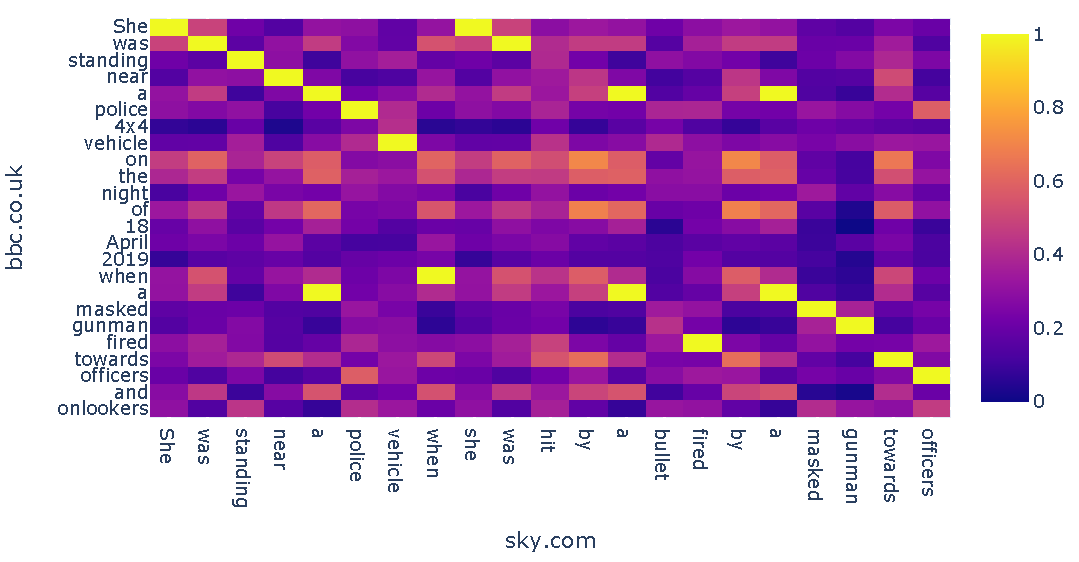
\includegraphics[width=0.9\linewidth]{figures/lyra.pdf}
    \caption{Difference analysis across similar sentences from BBC and Sky News.}
    \label{fig:lyra}
\end{figure}
% \todoHA{Table 3.2 and 3.3 refer to from text and explain}


With this kind of information on the number, type and magnitude of changes contained in different pairs of sentences, we can get a qualitative idea of how the measures of similarity coming from the different models are representative of the effective differences.
If we have two pairs of sentences, and the first pair contains bigger differences (count, magnitude) than the second one, we want the second pair to be ranked as more similar than the first one.
Therefore, if the model ranks the first pair of sentences as more similar than the second pair, that is a negative sign for that model. %\todoHA{And then what?}
% If a model scores more similar a pair of sentences that appear to us to be less related than another pair,\todoAW{Disturbingly vague!!} that is a negative sign for that model.
We can therefore understand how good the models are to rank the similarity of sentences, and make an informed decision about which model to consider for our work.


% Observations
% \todo{rewrite better the observations}
The main problem observed for the TF-IDF model is that it relies just on the terms. If two terms are interchangeable/synonyms, they are still considered as two distinct features. This is a big limitation considering that we are dealing with a wide multitude of documents,  %that deal with the same underlying events,
therefore we expect a big variance on the linguistical surface.
Then we have other technical observations for the TF-IDF model, for example, that the results change a lot depending on the feature size.
Furthermore, it requires to be computed on a set of documents all together (which also changes which features are selected), and it is not possible to encode an additional document without changing the representation of the already encoded documents because the term overall frequencies change.
We also see that the type of pre-processing affects the results: without a lemmatization step to the pipeline, it is sufficient to change the verb tense to have a different term.
Given these limitations, we find that sentences that are very similar in meaning but have some differences in the linguistic surface see a drop in their similarity with this model.

Instead, considering GloVe-average, we observe in some cases that the measure of similarity provided does not capture substantial changes in the meaning. The problem is that, while it can use wordwise similarity quite well, the sentence structure is not accounted for its representation. The representation is a simple average of the word vectors (e.g. ``Luke insulted John'' results in being equal to ``John insulted Luke''). %\todoAW{So this is a well known issue with VSM in general. How significant is it for the specific case you're looking at here?}
In our case, we need to be sensible to changes in the meaning even when the same words are used. The order of words may convey a different meaning and we want the similarity metric to capture this information.

For the language models (\acrshort{bert} and \acrshort{use} models), we see that the order given by the models is more aligned with what we consider to be the differences to be (second column of Table~\ref{tab:relative_ordering}).
What we do with this experiment is to try to make measurable something that is very qualitative (the similarity between sentences).
There exist already different benchmarks that are performed on the semantic similarity task~\citep{conneau-kiela-2018-senteval,chandrasekaran2021evolution}, and this experimentation is not trying to replicate them. Here we simply want to see how the different families of models compare on our task, where we need to understand the degree of similarity between related sentences and documents.

% a big improvement\todoAW{I'm not entirely sure at this point how you're evaluating the various methods} in the pairs of sentences that come as more similar.
% The values provided are very similar. This per-se is not a problem if some geometric properties are valid (ordering, proportions)
% We observe\todoHA{Many "observations" made here, but unclear how. Add some details if you can} that \acrshort{use} provides values less skewed to the higher end, distributing the similarity values more evenly.
Between USE and BERT, Table~\ref{tab:relative_ordering} shows that USE provides values less skewed to the higher end, distributing the similarity values more evenly. 
This is something very positive, because we want a metric that is able to tell degrees of similarity with a good granularity in all of the range.
% The numbers make more sense without any re-scaling technique, and therefore the heatmaps shown in this document\todoHA{?} come from this model.
We can directly use the values to produce heatmaps, without the need to re-scale the values. With BERT, it would be necessary as the values are all compressed in the higher end (near 100\% similarity).
Furthermore, USE is also the only model, among the four considered here, that is purposely trained on a semantic similarity task, while the other models can provide similarity measures just because of how they represent language.


% \todo{an example of two pairs where we can see some of the limitations?}

\begin{comment}
\subsection{\statusred Application to corroboration and omission extraction}
\label{ssec:cgs_similarity_cliques}
% Cliques with USE

\todo{This section needs some work still. Or otherwise remove it. Is it crucial to have this experiment?}
\todoHA{Can't tell yet. THe workflow of your thoughts and experiments need more clarification upfront in this chapter}

In this section, we take the experiment from Section~\ref{sec:cgs_cross_referencing} and substitute the TF-IDF encoding method with a semantic similarity model (\acrshort{use}).

While in the previous Subsection~\ref{ssec:cgs_similarity_qualitative} we were assessing the quality of USE vs TF-IDF on their own, here we see the difference when applying them to downstream tasks.


\todo{Show figure with USE, that results are better correlated?}

In figure\ref{fig:usebetter}, we can see that when we compare the base model TF-IDF with USE, we get a better correlation between corroboration and credibility.
% OR: we get unclear results.
% However, 
Show cliques inspection quality
when inspecting the cliques, we see that 

\todo{need an example}
\end{comment}

\subsection{\statusgreen Similarity Analysis Findings}
\label{ssec:cgs_similarity_conclusion}
% \todo{rename subsection or remove?}

% role of this experiment
This experiment shows the need for a similarity model that accounts for the semantics more than the linguistic surface. And given the continuous progress of language models, we need to be able to switch our choice relatively easily.
For example, by looking at the Semantic Textual Similarity benchmark,\footnote{\url{http://nlpprogress.com/english/semantic_textual_similarity.html}} at the moment the best model available is XLNet~\citep{yang2019xlnet} but this could change at any time.

For this reason, our following experiments use the USE model instead of the latest available models. The difference is not very big and we have the advantage of being able to compare our experiments without re-running all of them when a new model is released.

\acrshort{use} and XLNet both belong to the same family of models, so the differences between them should not be a big limitation of this work.

%so we will use it for our future experiments.
% this means for us:
% - we need to use a similarity resistant to changes in the linguistic surface
% - we need a measure that is able to represent well the different levels of similarity
% - we must be able to switch the model used easily, in case new public benchmarks for STS show a different winner (example XLNet~\cite{yang2019xlnet}).

%The purpose of this experiment is to have a good observation of how different types of models can be effective or not, and to experiment with them to drive the implementation of the processing pipeline.
% Benchmark, availability of code and maybe further measures on our system will decide the final ``winner''.
% Purpose: implementation and building of the pipeline.


\section{\statusgreen Fine-grained Differences Extraction}
\label{sec:cgs_clustering_and_differences}

% Experiment 3
% what
This section has two goals: 1) to improve the cliquing approach used in Section~\ref{sec:cgs_cross_referencing} and 2) to take a closer look at the fine-grained differences between highly-similar sentences and study the uniqueness of the words used.

% The next experimentation that we have done regards the usage of the similarity values to group together sentences describing the same details and at the same time study the uniqueness of the words used.

\subsection{\statusgreen Hierarchical Sentence Clustering}
\label{sec:cgs_clustering_and_differences_hierarchical}


% why
We have seen with the reproduction of the model from \citet{bountouridis2018explaining} that one big limitation of using cliquing techniques over unweighted graphs is that they do not exploit the full power of the distances available. This resulted in having fragmented clusters because the choice of the threshold is very sensible.
% We have also experimented with different embedding models and we want to use them
% \todo{from here on}
% This comes from the limitation of the first experiment of reproduction of the paper. (from experiment 1)
% (from experiment on similarity)

% how
With the idea to use clustering algorithms instead, we retrieved some groups of articles that relate to the same event from Google Headlines, which aggregates and clusters together news articles from multiple sources.\footnote{\url{https://www.blog.google/products/news/new-google-news-ai-meets-human-intelligence/}}
These documents are processed with the SpaCy NLP Python library\footnote{\url{https://spacy.io/}} to split the documents into sentences and have available different NLP functions (e.g., tokenisation, POS tagging).

% 1. distance computation
Each of the sentences is then passed through a language model which creates a sentence embedding, in this case using \acrshort{use} because it showed to distribute the similarity values more evenly and is specifically trained for sentence similarity.

% 2. hierarchical clustering (example with diagram)
We then use \acrfull{hac} for different reasons:
\begin{itemize}
    \item it does not require the specification of the number of clusters wanted, we want to be flexible;
    \item we can truncate the clustering when we reach a certain level of distance between the clusters, or a certain number of clusters;
    \item We can see the evolution of many different features (e.g., number of clusters, size, internal cohesion) while performing the clustering step by step;
    \item we have a graphical representation (dendrogram) which helps to inspect and understand what is happening;
    \item it has widely been used for similar tasks, e.g., finding related claims~\citep{almeida2020text}
\end{itemize}

% This clustering algorithm has the following parameters:
% \begin{itemize}
%     \item linkage method: how to choose which clusters to merge. Different strategies exist: Ward: minimise the total within-cluster variance (weighted squared distance between cluster centres). Single: Nearest Point Algorithm. Complete: Farthest Point Algorithm
%     \item distance function: cosine, euclidean, ...
% \end{itemize}
% \todo{describe why ward and cosine look better}

For this experiment, we consider a total of 20 different headlines, with an average size of 70 articles each.
After splitting the sentences, we have an average of 33 sentences for each article (total of 46373 sentences).
The \acrshort{hac} is done for each headline separately.

In Figure~\ref{fig:dendrogram}, we can see how different thresholds for sentence similarity would affect the generated clusters. The dendrogram on the right shows which sentences get in the same cluster at increasing distance values. Identical sentences are merged at the left of the dendrogram, with similarity close to $0$, while totally different groups of sentences get merged with higher values (near $1$ considering cosine distance).
% what is the distance required to have different sentences inside the same cluster,
%\todoHA{How these links were detected? How many sentences processed? Links context? Etc.} and select a certain threshold more consistently.
\begin{figure}[!htb]
    \centering
    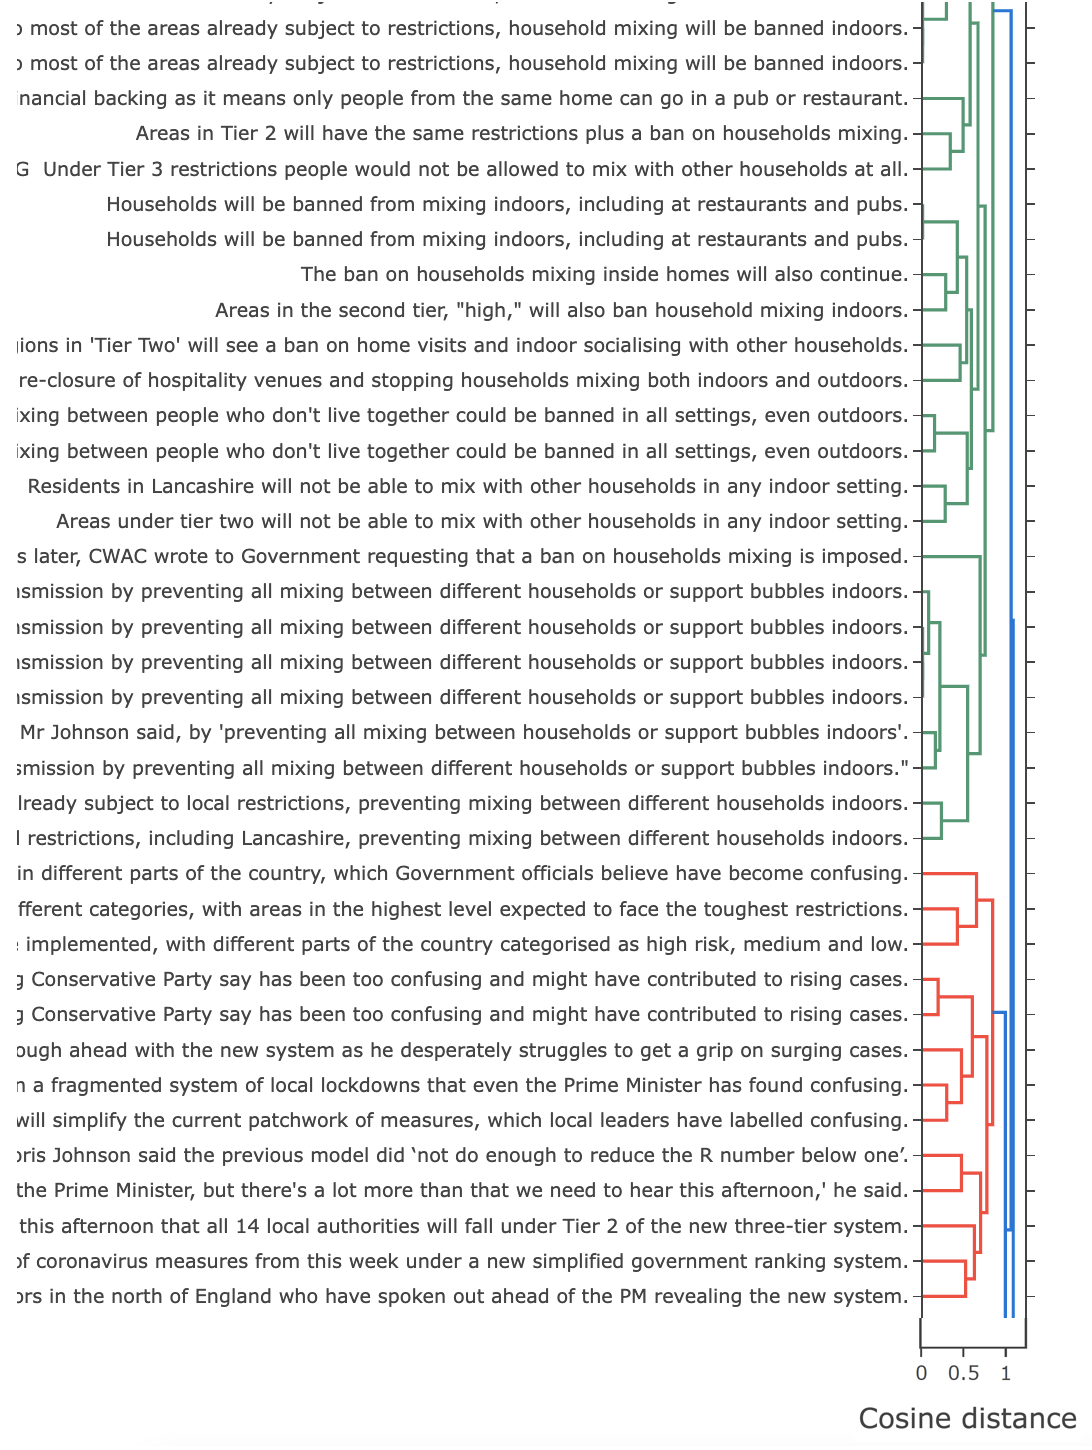
\includegraphics[width=\linewidth]{figures/dendrogram_high_legend.png}
    \caption{Partial dendrogram showing sentences merged by increasing distance.}
    \label{fig:dendrogram}
\end{figure}
% \todoHA{Put in a page by itself}

Using this type of inspection, we can decide specific threshold values that make ``similar enough" sentences go into the same cluster, while keeping other sentences in other clusters.
%we can see what is the required similarity to make two pairs of sentences be in the same cluster.
% \todo{some observations about the distance values and threshold}

% 3. extract degree of uniqueness of words (from pairwise to clusterwise, with bag-of-words or difftool (order matters, duplicates))
% second motivation: highlight the different words and their uniqueness
With this method, we can create sentence clusters that are very similar in their semantic content, but at the same time have linguistic changes. This is a joined effect of having models that deliver a better similarity metric and also of applying a weighted-similarity approach when building the clusters and not just a binary approach (as done instead with a cliquing algorithm instead of clustering ones).

\begin{figure}[!htbp]
    \centering
    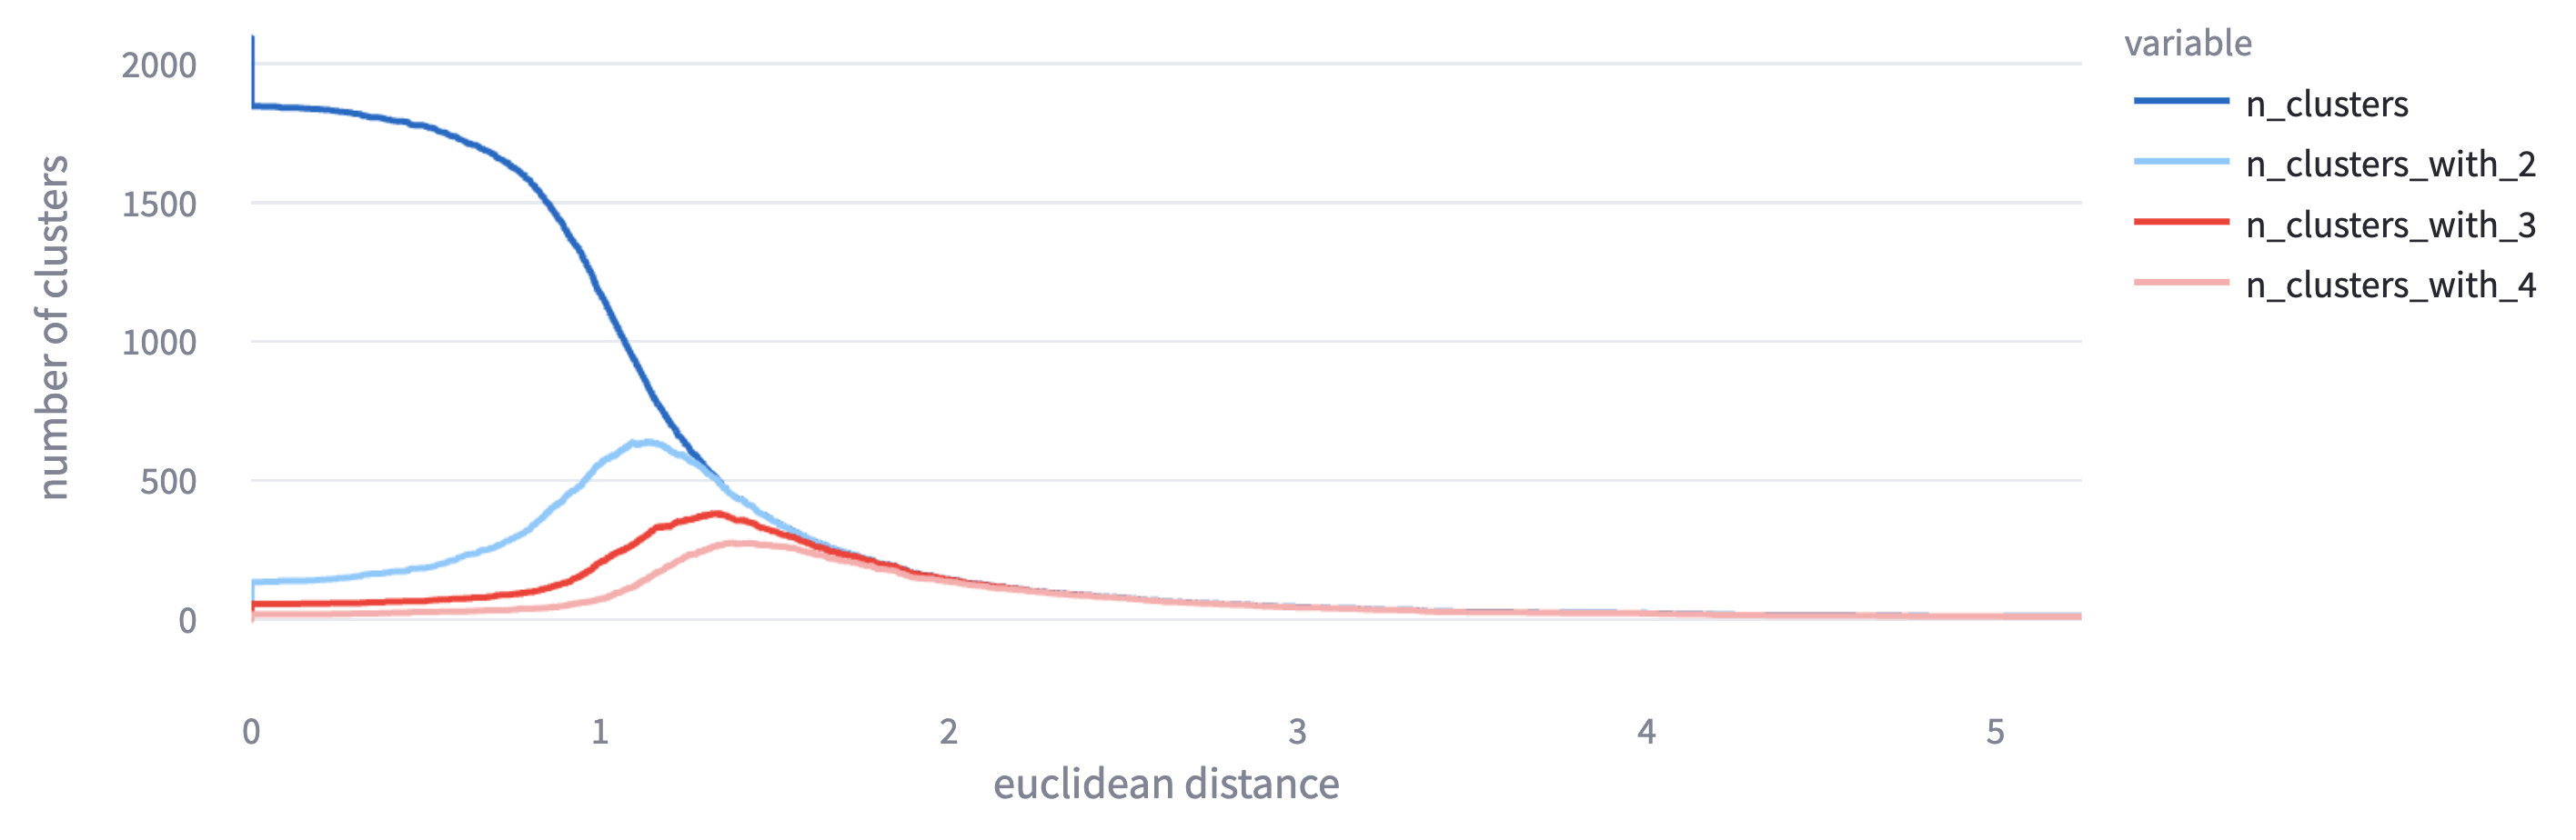
\includegraphics[width=\linewidth]{figures/clusters_count_by_threshold_bigger_2.png}
    \caption{
    Clusters of different minimal sizes with increasing distance thresholds.
    %Number of clusters (with minimal size of 1,2,3,4) plotted when the distance threshold varies. The blue line counts also for sentences that are on their own, while the others lines are more and more stricter with the number of sentences per group to be counted.
    }
    \label{fig:clusers_count_by_threshold}
\end{figure}
% \todo{improve figure: re-export, set limits, scale}
In Figure~\ref{fig:clusers_count_by_threshold} we see how the number of clusters evolves when we increase the similarity threshold. 
The dark blue line indicates all clusters, counting also clusters with just one sentence inside.
On the blue line, we notice a steep drop at distance next to $0$: this denotes that there are lots of sentences that are identical or just differ in punctuation.
A second drop happens around the Euclidean distance of 1.
Then, with the other lines, we represent clusters that have stricter conditions in terms of the minimal number of sentences per cluster. We respectively only count clusters with 2, 3 and 4 sentences minimum.
All these lines have a similar behaviour: with the distance increasing, they increase to reach a maximum (because new clusters are formed satisfying the minimum number of sentences) and then decrease again (because the clusters are merged together, so they are less). 
The peak is reached with Euclidean distance around $1.2$.
Notice that with respect to the previous dendrogram plot, here we are using Euclidean distance to show values less compacted together.
The value of $1.2$ Euclidean is observed across the different headlines to consistently provide clusters with a good variation of terms but still having a strong semantic connection (e.g., same details, same entities mentioned).
Therefore, we use this value in the following Subsection~\ref{sec:cgs_clustering_and_differences_uniqueness}.

% By also inspecting several dendrograms, we consistently notice that around that interval, $0.55-0.65$ Euclidean distance, we are able to capture good variations on the surface form but the meaning of the sentences keeps similar.
% Therefore, we select the value of $0.6$ as our threshold for the next subsection~\ref{sec:cgs_clustering_and_differences_uniqueness} (the example shown in it have this parameter).


% \todo{How do we know this is better than cliques? Ground truth of clusters is not available. A benchmark test would be required to claim superiority. Do we need to repeat the initial experiment with this clustering instead of cliquing?}
% \todoHA{Important question to be discussed. Need to evaluate, if not quantitatively then qualitatively}
% \todoAW{Does such a benchmark test exist anywhere? eg. for other domains?}
From a qualitative analysis of the generated clusters, we find that this methodology produces better sentence clusters with respect to the method described in Section~\ref{sec:cgs_cross_referencing}.
We do not find many examples of sentences belonging to the wrong cluster, and we are able to find word variations that do not cause a major change in meaning.

With the sentence clusters produced, we move to the following Section, where we analyse the variations at the word level.

\subsection{\statusgreen Term Uniqueness}
\label{sec:cgs_clustering_and_differences_uniqueness}

With the outputs of the sentence clustering from the previous section~\ref{sec:cgs_clustering_and_differences_hierarchical}, we want now to take these sentences, which should be similar in the meaning but with some variations on the linguistical form, and analyse how they overlap or not in the terms used.

% What we want to achieve, is to have a good way to analyse the fine-grained differences between the extracted similar sentences.\todoHA{What? What's the final goal?}
Therefore, our final goal for this experiment is to compute the uniqueness of words across multiple variations of describing the same detail.
One news source may be using completely different terms from the others, or share with others the same terminology.
This word-level analysis completes the corroboration and omission analysis, which instead is performed at the sentence level.

To facilitate an analysis of the differences, we experimented with different methods of highlighting the uniqueness of the words in a cluster.
Inspired by software engineering tools, we first tried with algorithms based on \texttt{diff}~\citep{myers1986ano}.
% Diff (also coming in UNIX distributions under the \texttt{diff} tool)
\texttt{Diff} is a great algorithm and UNIX tool for comparing different modified versions of the same document.
This algorithm is also able to detect changes in the position or ordering of elements. This aspect is not very important in our analysis, because natural language is more flexible and reordering phrases and sub-phrases should not be accounted for in our analysis. So with the relaxed constraint on the position of the words, we moved to a measure of term uniqueness based merely on the words appearing or not in the considered sentences. For this reason, we named this comparison \texttt{set-based} instead of \texttt{diff-based} because we treat the words for each sentence as a set (without considering the position and repetitions of words).
Although we do not consider repeated words in a sentence as modifying the uniqueness of terms, we will still take into consideration repetition as a persuasive technique in the next chapter.

We therefore define a scale of uniqueness in the following way:
$$u_w = 1 - \frac{|\set{s_i | s_i \in S \land w \in s_i}|}{|S|}$$
where $S$ is the set of sentences considered, $w$ is the word for which to compute the index. The expression compares the sentences of the current cluster where $w$ appears (numerator) with respect to the cluster size.
A value close to $1$ means that the word is used in just a few sentences in the cluster.

In Figure~\ref{fig:words_uniqueness} we can see an example of this metric applied to a cluster of three sentences.
For each word, the uniqueness score is computed, and then we associate the values to a colour scale.
In this way, we can instantly see the words that are most unique and the ones that instead are repeated across multiple sentences.
In this case, the word ``deceased'', which just appears in one of three sentences, gets assigned a high value of uniqueness ($u = 2/3$). Instead, the word ``surgery'', which appears in all three sentences, has $u = 0$.
% \todoHA{You mean overall or in this example?}

\begin{figure}[!htb]
    \centering
    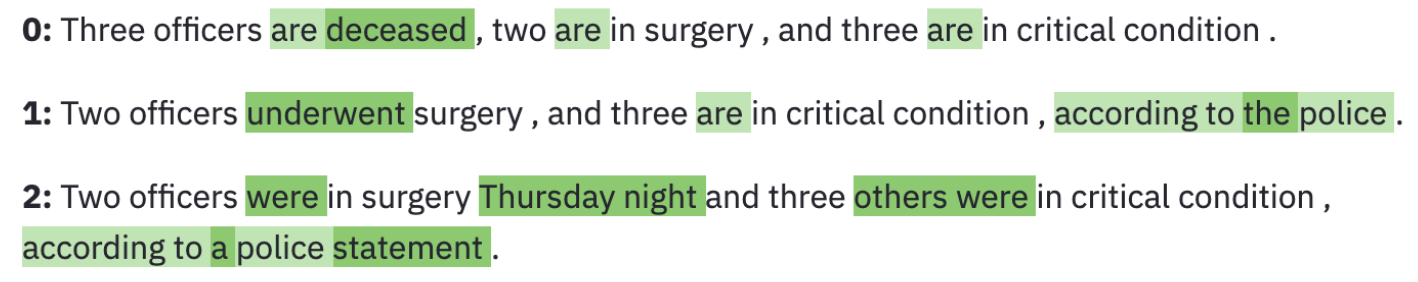
\includegraphics[width=\textwidth]{figures/words_uniqueness.png}
    \caption{A sentence cluster example highlighting the uniqueness of words.}
    \label{fig:words_uniqueness}
\end{figure}


% not only uniqueness, but how it was used to observe variations of terms
This uniqueness was used to inspect around 25 sentence-level clusters that were gathered by using the \acrshort{hac} as described in Section~\ref{sec:cgs_clustering_and_differences_hierarchical}. Helped by the uniqueness degree of the words, we are able to spot the differences between the sentences faster and classify the main types of singular words that change:
\begin{enumerate}
    \item verb tenses: not meaningful in this context
    \item chunks of information at the beginning or end of the sentence. Usually, those pieces are just a matter of segmentation of the sentences (e.g. the reporter actually includes the omitted terms in the next or previous sentence) 
    \item details that are present in some articles and omitted in others (e.g. Figure~\ref{fig:words_uniqueness})
    \item verb choices across synonyms
    \item substantive/adjective choices across synonyms
\end{enumerate}

Across these types of changes, we are particularly interested in the term choices (verbs, substantive, adjectives) as they are the details that may mostly change the message transmitted to the reader.
With this methodology that is only based on similarity and overlap analysis, we are not able to tell more about these term choices. We need external analysis that will be faced in the next Chapter.

\subsection{\statusgreen Meaning of Fine-grained Differences}
% TODO: findings?
The experimentations shown in this section have two directions that seem to be opposing: 
\begin{itemize}
    \item On one side (similarity), create clusters of sentences accordingly to their semantic similarity using a more flexible hierarchical clustering (to capture similar-enough sentences). %(more broad and resistant to changes in the linguistical surface)
    \item On the other side (differences/uniqueness), to be able to extract and see how the word-level details change.
\end{itemize}

It may look like a contradiction, but we need this double analysis to link different sentences that share the same stories and to be able to see the actual differences between them.

With this approach, we are able to see in details which words have changed in sentences coming from different news sources.
With comparison to the approach presented in~\citet{bountouridis2018explaining}, we are now able to see more granularly than just at the document and sentence-level.
There are several ways in which the selection of what to include or to exclude in an article may show facts under a different light. Not only we are able to see which details corroborate or have been omitted (Agenda-setting~\citep{Cohen_1964}), but we identify single terms which can reveal the intention to persuade or to push for a certain interpretation by the writer. Seeing these terms, and the alternative terms used by articles on the same topic, could enable us or the reader to get awareness of the possible influence of the point of view of the writer or news outlet.

However, we see that many variations of terms do not seem to carry any differences in the perspective of the writer. Some others instead, convey a message very differently from a few words. Similarity alone cannot distinguish between them. And in this chapter we do not have the tools to quantify this phenomenon. A we will describe in the last section of this chapter, we need to experiment with the work of persuasion detection (next chapter).



% role of this experiment and outcomes
% This methodology can be used in our framework to help the preparation of the dataset in different steps.
% First of all, during the creation of article couples that have to be compared (using at the article-level the same clustering methodology). In this case, we will need to use a specific threshold that cuts out unrelated articles but at the same time keeps a considerable number of differences on the document level (not too similar because identical articles, that are a lot, are not useful).
% While for the first user study we can exploit hand-curated groups of articles, when doing a larger creation of the dataset we will need to rely on automated techniques.
% This methodology could also be used as support for the annotators, to see both which sentences are most similar, and the words that differ inside. This would make the annotation process faster and easier.

% This experiment needs to be completed, to choose some parameters with better criteria. We want to identify good intervals for the thresholds and parameters (e.g. with euclidean distance around 0.6-1.0 sentences start to have linguistic variations but still very related to the same concepts).

% This experiment evidences the need to explore more on the interpretation of the differences, pushing for the user study of RQ1.1.

% It serves the RQ1.2 as a first implementation of the processing pipeline by making available different articles and their document and sentence-wise relationships. Building on top of these features, we can then develop the methodology for doing the cross-article framing analysis.



\section{\statusgreen Discussion}
\label{sec:cgs_findings}

% From this chapter, we achieved to be able to understand and study when information is unique or shared between different news sources, at different granularities:
% \begin{itemize}
%     \item article-level: finding related articles that cover the same events;\todoHA{Which section shows these results?}
%     \item sentence-level: being able to find the sentences that corroborate, the ones that are unique or omitted;
%     \item word-level: computing the degree of uniqueness of single terms, and observing how single words are changed between multiple sources.
% \end{itemize}

% \todo{I need something to link together this chapter and also need strong findings to conclude it.}

This chapter had several sub-questions, that we discuss separately here, before discussing the overall RQ1:

\begin{enumerate}[label={\textbf{RQ1.\arabic*:}},leftmargin=2cm]
    \item \emph{How are new events reported differently by multiple sources?} News sources present the same event in different ways, including different details that corroborate with other sources, omitting details that other sources instead report, changing the order of presentation of the details. We studied and measured these phenomena in this chapter, but we deem it necessary to study the choice of terms, by investigating what is the reason and what is the effect of deliberate or involuntary choices. We will expand on this in the next Chapter.
    \item \emph{How could we identify what is unique for each report and what is common?} To identify what is unique, common or omitted, it is possible to use the methodology of~\citet{bountouridis2018explaining} to detect omission and corroboration, %(Section~\ref{sec:cgs_cross_referencing})
    which is based on splitting the articles into sentences and comparing them with similarity metrics.
    % We extended the approach to analyse at the word level the variation of terms across multiple related articles, and compute the relative uniqueness of terms 
    We went one step further, by being able to automatically find the specific words that change between multiple news articles, and identify the degree of uniqueness of them (Section~\ref{sec:cgs_clustering_and_differences}). We think that this is potentially beneficial for many downstream tasks, such as showing to the user during annotation tasks or even when consuming news online.
    \item \emph{To what extent can we automatically detect omission and corroboration across multiple articles?} The approach, identified to answer the previous \acrshort{rq}, works better for detecting small differences between articles that have several parts in common. When the articles are too different, for example, if they consider totally different events or if the overlap of terms is too small, it becomes difficult to align the documents with similarity metrics and the results are less meaningful. We also find that our analysis is able to find terms that change but does not give an interpretation of what these changes mean. For example, we cannot currently distinguish between a loaded term versus a more neutral one. For this to be possible, we need the study of persuasion means (as discussed in RQ2).
    \item \emph{Which similarity metrics are best for detecting omission and corroboration?} We underlined in Section~\ref{sec:cgs_similarity} the importance of using semantic similarity metrics that go beyond the binary comparison (equal or different) of terms. In this way, we are more resistant to term changes and can identify better the related sentences across articles.
\end{enumerate}

We can now answer our overall RQ1: \emph{To what extent do news articles about the same events differ?}

After comparing news articles covering the same events, we discovered that they can vary in several ways. Firstly, some articles may omit certain details while others confirm them. Secondly, different terms may be used to express the same detail. While it is relatively straightforward to analyze the first type of difference using similarity metrics, it is not sufficient for understanding the nuances of the second type. We need in this case to analyse the terms involved to go beyond the simple differences.


% The main findings that we have from this chapter are the following:

% \begin{itemize}
%     \item As already denoted by the work of~\citet{bountouridis2018explaining}, we confirm a positive correlation between corroboration and credibility of news outlets and a negative correlation between omission and credibility. We went one step further, by being able to automatically find the specific words that change between multiple news articles, and identify the degree of uniqueness of them. We think that this is beneficial for many downstream tasks, such as showing to the user during annotation tasks or even when consuming news online. %: corroboration correlates positively to credibility of news outlets, omission negatively
%     % \item Extreme left and right corroborate less and omit more? (but needs leaning? No if we just take centrality-extremism)
%     % \item Delta Time of publication: more similar articles are published at similar times, instead the further the time delta the more further they are?
%     % these are more limitations
%     \item Observing similarities between multiple documents is made very difficult by linguistic variations. We experimented with models (e.g. \acrshort{use}) that are more resistant to words that carry similar meanings and are a better fit for doing this type of analysis. %It is not only a matter of what is included and what is excluded. The similarity between sentences is also capturing some linguistic variations more than others (more about the surface and less about the intention).
%     \item We do not have any interpretation of what a change in a document conveys. Something may be written differently just because of random choices, or there can be some hidden reasons and some goals to persuade. The similarity computation, necessary to understand how the documents overlap or not, gives no understanding of the persuasion means and the intention behind specific choices. This will be explored in the next Chapter~\ref{chap:linguistic_persuasion}.
% \end{itemize}



\section{\statusgreen Next}
\label{sec:cgs_next}
% link to next chapter

This chapter gives us some insights into how similar documents are changed and modified across news sources, and how critical corroboration and omission are.

% recap contributions? (done before already)


% open for new chapter
However, what these changes \emph{convey} remains unclear.
It could be that the differences exist for different natures, originating from randomness (each author/source has different jargon, or by casualties).
On the other hand, there could be a purpose that is subtly manifesting through these small choices. This purpose could be to influence the readers, with persuasion or manipulation.

This chapter raised some questions that need to be answered:
What changes between the changed parts? What characterises those differences? How can we characterise the differences quantitatively, describing how they try to persuade the readers? To give an answer to these questions, we need to include in our analysis some concepts of persuasion.

Therefore, in the next chapter we will investigate persuasive language and how it can be computationally quantified. 


\chapter{\statusgreen Linguistic Techniques of Persuasion}
\label{chap:linguistic_persuasion}

\section{\statusgreen Introduction}
\label{sec:lp_intro}

% what (orientation)
In this second experimental chapter, we introduce a new ingredient in our analysis: persuasion techniques.
\todoHA{wasn’t this already introduced in chapter 3?}
With the previous Chapter~\ref{chap:common_ground_search}, we underlined our need to understand how different terms, that are used to describe the same details, can effectively convey a different message to the readers.
Therefore, in order to characterise those differences, this chapter introduces \gls{persuasion} as an umbrella term that encompasses several techniques where the writer of a piece of text is trying to push to the reader a certain point of view.
% In this chapter, we add our second ingredient: persuasion.\todoAW{abrupt start}
% We intend persuasion as a general umbrella that encompasses several techniques where the writer of a piece of text is trying to persuade the reader of a certain point of view.

% why (rationale)
From the last chapter~\ref{chap:common_ground_search}, 
%we concluded with the need to understand how specific terms are used to persuade the reader. 
we are able to extract terms that have been changed in related articles, from sentences that are very similar but have still some differences.
Our aim is here to quantitatively analyse these detected variations to quantify their specific use of persuasion techniques.
% \todoHA{Why? What is the value of this detection?}
In this way, we could understand if the specific term choices are in fact done to persuade the reader of a specific idea, or if they are only the manifestation of random choices.

For this reason, this chapter investigates the \emph{linguistic techniques of persuasion}, in other words, how the persuasion manifests itself on the linguistical surface.
% aim
Our motivation is to analyse whether the terms that change between multiple articles/sentences are correlated with the linguistic techniques of persuasion.

The Research Questions for this chapter is \acrshort{rq}2: \emph{To what extent can we automatically detect the persuasion techniques used in news articles?} It is split into four subquestions:
\begin{enumerate}[label={\textbf{RQ2.\arabic*:}},leftmargin=2cm]
    \item To what extent could we automatically detect the persuasion techniques used by writers? % Which are the possible indicators of these differences? // 
    \item Which persuasion techniques are detected more frequently than others?
    \item How do similar news articles differ in their use of persuasion techniques? %\emph{How are the differences between similar articles} (extracted in the previous chapter) \emph{related to a different use of persuasion techniques?} % Is there a link between the parts that are different and persuasion techniques (propaganda/loaded language)? // 
    \item To what extent could persuasion techniques be used to identify related news articles?%If the same story can be narrated differently depending on the persuasion techniques used, then persuasion is adding variations to the narration. Therefore, \emph{how much of an obstacle is persuasion in recognising articles that are related to the same news?} %(clustering) % how much of an obstacle is persuasion in recognising the events in multiple articles?
    %\todoHA{What led to this RQ? Previous text does not lead to this}
\end{enumerate}


% method
% strong/loaded language: using sentiment analysis tools 
% 18 techniques of propaganda

% Experiment together with common ground search
To answer these research questions, we take from Chapter~\ref{sec:lit_persuasion} the most commonly and recently analysed \gls{persuasion} techniques for which computational detection methods exist: \gls{propaganda} and \gls{sentiment}.
%\todoAW{Slightly weird phrasing here... have you run this through Grammarly?}
%\todoHA{Any refs that link propaganda and sentiment with persuasion?}
% \todoAW{Harith asks what links propaganda, sentiment and persuasion. I'd ask what separates them. ie. why do you need to study persuasion at all if you can detect the other two cases?}
% \todomargin{MM: Persuasion including both, needed a term to simplify instead of always saying propaganda and sentiment}

% BEGIN response to HA
As discussed in Chapter~\ref{sec:lit_persuasion}, we consider here \gls{persuasion} as a term that encompasses both \gls{sentiment} and \gls{propaganda}. % and populism
It is linked with sentiment because of its goal to influence the emotional response~\citep{gatti2014sentiment,rocklage2018persuasion,petty2015emotion,desteno2004discrete}.
The relationship with propaganda comes from the inherent goal of propaganda to influence the view of the public about an idea or a group~\citep{bernays,jowett2018propaganda}.
%\todoAW{Good early citation shows you're aware of the broader literature... do you have others elsewhere in the dissertation? If not, probably worth making sure you're aware of some of the key authors in the area. Three or four should be enough.}

% It is known that persuasion is related to an emotional response from the reader/listener, being related to emotions.
% Persuasion and Discursive Repertories~\cite{orrumachine}
% propaganda is a``consistent, enduring effort to create or shape events to influence the relations of the public to an enterprise, idea or group''~\cite{bernays}.
% Persuasion and Propaganda: ~\cite{jowett2018propaganda}.
%, populism.
% END response to HA


% carry the following experiment:
Therefore, after describing the used datasets in Section~\ref{sec:lp_datasets}, we have the first part of this chapter that covers the detection of these persuasion techniques (Section~\ref{sec:lp_techniques}).
Afterwards, in Section~\ref{sec:lp_relationship} we put this in relationship with the analysis from the previous Chapter~\ref{sec:cgs_clustering_and_differences}. % Chapter~\ref{chap:common_ground_search}
We extend the study to consider the terms that change between articles, and we analyse whether they are associated with some persuasion techniques, and in what way. %indicate something about the changes in the sentences.

In order to achieve this goal, we consider in this chapter the following processing pipeline:
\begin{enumerate}
    \item Analysis from Chapter~\ref{chap:common_ground_search}: extracts the words that are changed between similar sentences of similar articles.
    \item Extraction of different techniques (sentiment, propaganda) on the sentences (described in the next Section~\ref{sec:lp_techniques}). %\todoAW{Doesn't your earlier paragraph suggest that we've already got this? ("means for which we have computational detection methods: propaganda and sentiment"))}
    \item Analysis of the relationship between these techniques and the changes in the sentences (described in Section~\ref{sec:lp_relationship})
\end{enumerate}


% findings
We discover that
the initial methods for fine-grained propaganda detection seem to be more promising %\todoHA{How? In what way?}
than sentiment detection.
Fine-grained propaganda analysis gives a multidimensional result because it provides the amount and words for each specific technique. Instead, sentiment only provides a mono- (or bi-) dimensional result. Furthermore, it shows weaker results, as will be shown in the next sections: sentiment detection produces many words that are \emph{false positives}, and it becomes more difficult to understand which outputs we can rely on.
% Sentiment is (cor)related to the specific propaganda technique of \texttt{Loaded\_language}, and having one technique instead of $18$ is only a disadvantage.
% does not provide useful insights when observed together with the changes occurring in the articles. 
The multi-dimensionality of propaganda across the techniques is much more useful and also more precise.
For this reason, we mainly use propaganda for the experiments of the following chapters. 
% \todoHA{I agree with AW. 
% also, you had a pipeline in the previous version. why removed? 
% good to tell the reader what steps you’ll be taking and why, before getting into all the detail. 
% }

% pointers to next sections
% The next sections are organised as follows. Section~\ref{sec:lp_techniques} contains the analysis of persuasion techniques: sentiment and propaganda.
% \todoAW{You've already told me this...}
% %some techniques that we identifed being related to persuasion.\todoAW{? I don't know what you mean by "related to" here.}
% We present what they are able to detect on our datasets. %(stage 2 of the pipeline above described).
% Then Section~\ref{sec:lp_relationship} contains two experiments aimed at understanding the relationship between these techniques and the words changed.%(stage 3 of the pipeline).

\section{Datasets}
\label{sec:lp_datasets}

In this chapter, we make use of several datasets. 
First, we use them to understand how the detection of persuasion techiques works: Section~\ref{sec:lp_techniques} covers sentiment and propaganda detection, and we use different datasets to get some statistics about the detection itself.

Then, in Section~\ref{sec:lp_relationship}, we have two different experiments that cover the relationship between persuasion techniques and variations between similar articles.

Some of these datasets were already used in the previous chapter, and some of them are instead being generated with the methodology described in the previous chapter.

% \subsection{Sentiment analysis}

% % Datasets: AllSides, AllNews
% First of all, as described also in the previous chapter, we rely here on two datasets: AllSides and AllNews.

\subsection{AllSides}

The first dataset that we use, as in the previous chapter, is AllSides.
% \todoHA{so not all datasets here are different. you. may want to change the earlier statement then to be more accurate}
This dataset contains articles that are grouped in “headlines” (3 articles for each headline) and each headline belongs to one of the 326 topics (almost all political-related). There are (updated 26th October 2022) 5124 headlines, for a total of 15050 articles. They are grouped in triples, called \emph{headlines}. Each triple belongs to one of several topics, which can be seen as more loosely-grained clusters. 
As positive side, it is human-curated,\todoHA{rewrite more clearly}
meaning that it is not the result of an algorithm (like Google News) but some curators manually grouped the articles. Therefore, the groups of articles could be considered of high quality.
\todoHAinline{note that we can't say for sure since we know nothing about who these curators are, how many contributed to the grouping, did they disagree or not, etc. We assume quality since this is a public and known website but we need to do some evaluation to be more certain. This could go into your discussion section.}
Furthermore, this resource is publicly available, as the AllSides website provides the Headline Roundups.\footnote{\url{https://www.allsides.com/headline-roundups}}

On the negative side, although the data is public, it is licensed and furthermore the articles are just linked and not included.
This means that for collecting it, we need to manually retrieve the contents of the pages externally linked, which incurs in additional scraping problems and licensing problems.
\todoHAinline{the license issue is not related to this analysis, so move it to the discussion section. As for the need to collect the articles, again, this is not a negative side. It's just a task you need to do. Try not to throw negativity into your work so early on. Rewrite}
Another negative side,\todoHA{this is a limitation, not a negative side}
is that there are only three articles for each headline, so we do not expect to find a lot of linguistic variations, especially if we are strict on only having highly similar sentences. For this reason, it would be difficult to use it on the experiment detailed in Section~\ref{ssec:lp_relationship_small_variations} that requires fine-grained difference analysis.
Instead, we use it on the experiment of Section~\ref{ssec:lp_relationship_removing} that works on the article level only.
% sides: human-curated, public. Negative sides: only 3 articles for each headline. But for each topic, there are 46 articles on average.

\subsection{All-the-News}

Another dataset that we use throughout this chapter, is \emph{All-the-News}.\footnote{\url{https://www.kaggle.com/datasets/snapcrack/all-the-news}}
As described in the previous chapter, this dataset includes more than 140k articles published by fifteen major US outlets.
% The second one, AllNews, is much larger as it includes 2.7 million news articles, published between January 2016 and April 2020.\todo{finish} --> new version has milions

% Something specific for this chapter: used because it has larger quantity of articles
Therefore, we use it because it has a larger quantity of articles than AllSides. We use it in Section~\ref{sec:lp_techniques} to do a larger analysis of how the detection of the persuasion techniques works.

However, it has also some disadvantages, as the articles are not grouped together by topic or headline.
This means that this resource is less suitable for the experiments in Section~\ref{sec:lp_relationship}, that instead need to start with groups of articles.

\subsection{Small Variations Dataset}
\label{ssec:lp_relationship_small_variations_data}

Here we introduce our own dataset, that is created to analyse the small variations between similar sentences.
This dataset is derived from Google News Headlines (described in the previous chapter), and consists of pairs of sentences (extracted from the analysis of chapter~\ref{chap:common_ground_search}) which are characterised by high similarity score (\acrshort{use} model).

The dataset of origin is Google News Headlines, as it presents clusters of articles with a high number of articles each (between 20 and 90). Therefore, applying the methodology described in Section~\ref{sec:cgs_clustering_and_differences}, with quite strict thresholds on the distance between sentences, we can still produce in output many groups of sentences. These groups contain sentences that have minimal variations, and in Section~\ref{ssec:lp_relationship_small_variations} we aim to understand how these variations are related to a different usage of persuasion.
% Google headlines: articles are grouped in clusters. Clusters have around 20-90 articles each. Each cluster belongs to a certain broader topic (UK, World, Business, Entertainment, Sports, Science, Health). Positive sides: very large. Negative side: the clusters change over time, they are created by ML (not human-curated)

The Google News Headlines that we selected are between 8th September and 14th October 2020,
%\todoAW{OK, but be prepared to talk about whether you should have done a later version of the experiment. That will be a minimum of 2 1/2 years prior to the viva.} 
because that is the timespan during which this experiment was conducted, but it could be repeated in other timespans.
We extracted from them a subset of 138 sentence pairs, by using the approach described in the previous Chapter~\ref{sec:cgs_clustering_and_differences}:
\begin{enumerate}
    \item Random headlines (groups of articles) are selected. Their articles are segmented into sentences and each sentence is embedded with the \acrshort{use} model.
    \item Groups of sentences are extracted using \acrfull{hac}, to be able to use a similarity threshold to cut the dendrograms at any point. The features are the embeddings of point 1.
    \item We select thresholds for the clusters: minimal of $80\%$ and maximum of $98\%$ cosine similarity. In this way we select sentences that are related to the same detail (discarding sentences that are too different), but at the same time we discard sentences that are almost identical and only differ by punctuation.
    \item We randomly select a small subset of sentence pairs. From each cluster of sentences (containing three or more), only two sentences are selected in order to avoid having three-way comparisons (or even higher grade).
    %\item Manual annotation of whether the differences in the sentence pairs are making use of different persuasion or relate to a different opinion / point of view. This specific data is used for the experiments ``comparison with manual annotations" at the end of this Section~\ref{ssec:lp_relationship_small_variations_qual}
\end{enumerate}

Figure~\ref{fig:raw_clique_data} shows an example drawn from our dataset. We can see how the same detail has been phrased differently by different news articles.
The last sentence was removed because it was $100\%$ similar to the third one, and we only accept similarities in the range $[80\%,98\%]$.

\begin{figure}[!htbp]
    \centering
    \fbox{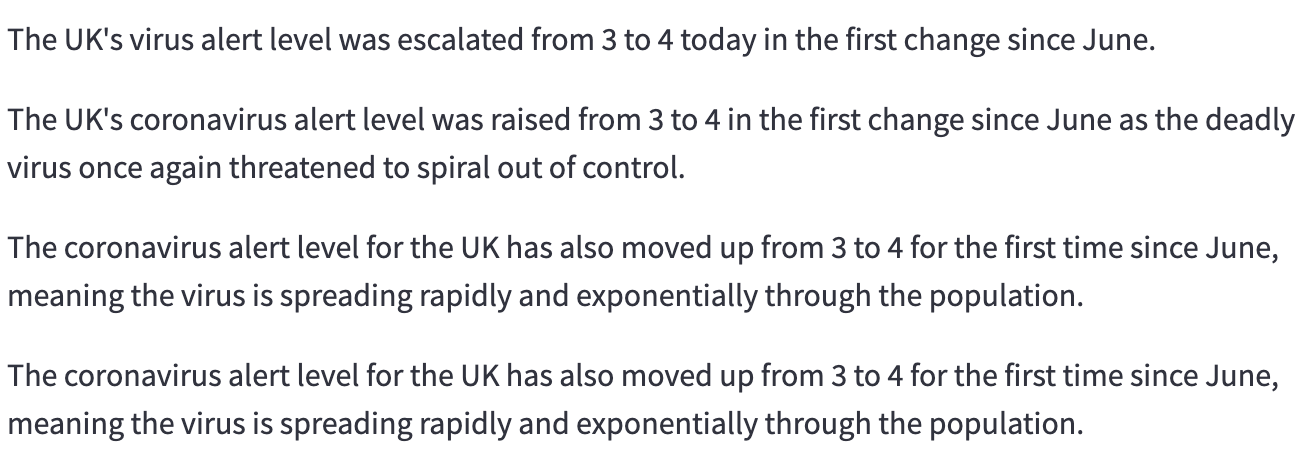
\includegraphics[width=\linewidth]{figures/annotation_212_raw_with_duplicate.png}}
    \caption{Example of a cluster of sentences that we used to build sentence pairs.}
    \label{fig:raw_clique_data}
\end{figure}






\section{Different Techniques of Persuasion}
\label{sec:lp_techniques}

% TODO preamble to different techniques: sentiment, propaganda, populism, ...

From all the different methods and approaches described in Chapter~\ref{sec:lit_propaganda}, in this section, we are using a set of methods to detect phenomena related to persuasion. % and do that at the word-level.
In other words, we are detecting several techniques that are considered 
%\todoHA{Assume? No references to support this assumption} 
to be related to persuasion~\citep{gass2018persuasion}: sentiment and 18 different propaganda techniques.% and populism.
%\todoAW{I imagine that there's probably quite a lot of linguistics literature in this area that you should look at, if only to pin down your terminology. → easier to work out the terminology. At the moment I have persuasion (as top) then prop/sentiment/ that are subclasses. Look in literature.}


When selecting which techniques to target, we have an important requirement to keep in mind: we are interested to work at the word-level, because our end goal is to study how persuasion techniques relate to the variations across the articles (as will be seen in Section~\ref{sec:lp_relationship}). Only having a score for the whole article or for a whole sentence is insufficient, because we need also word-level information.

\begin{figure}[!htbp]
    \centering
    \fbox{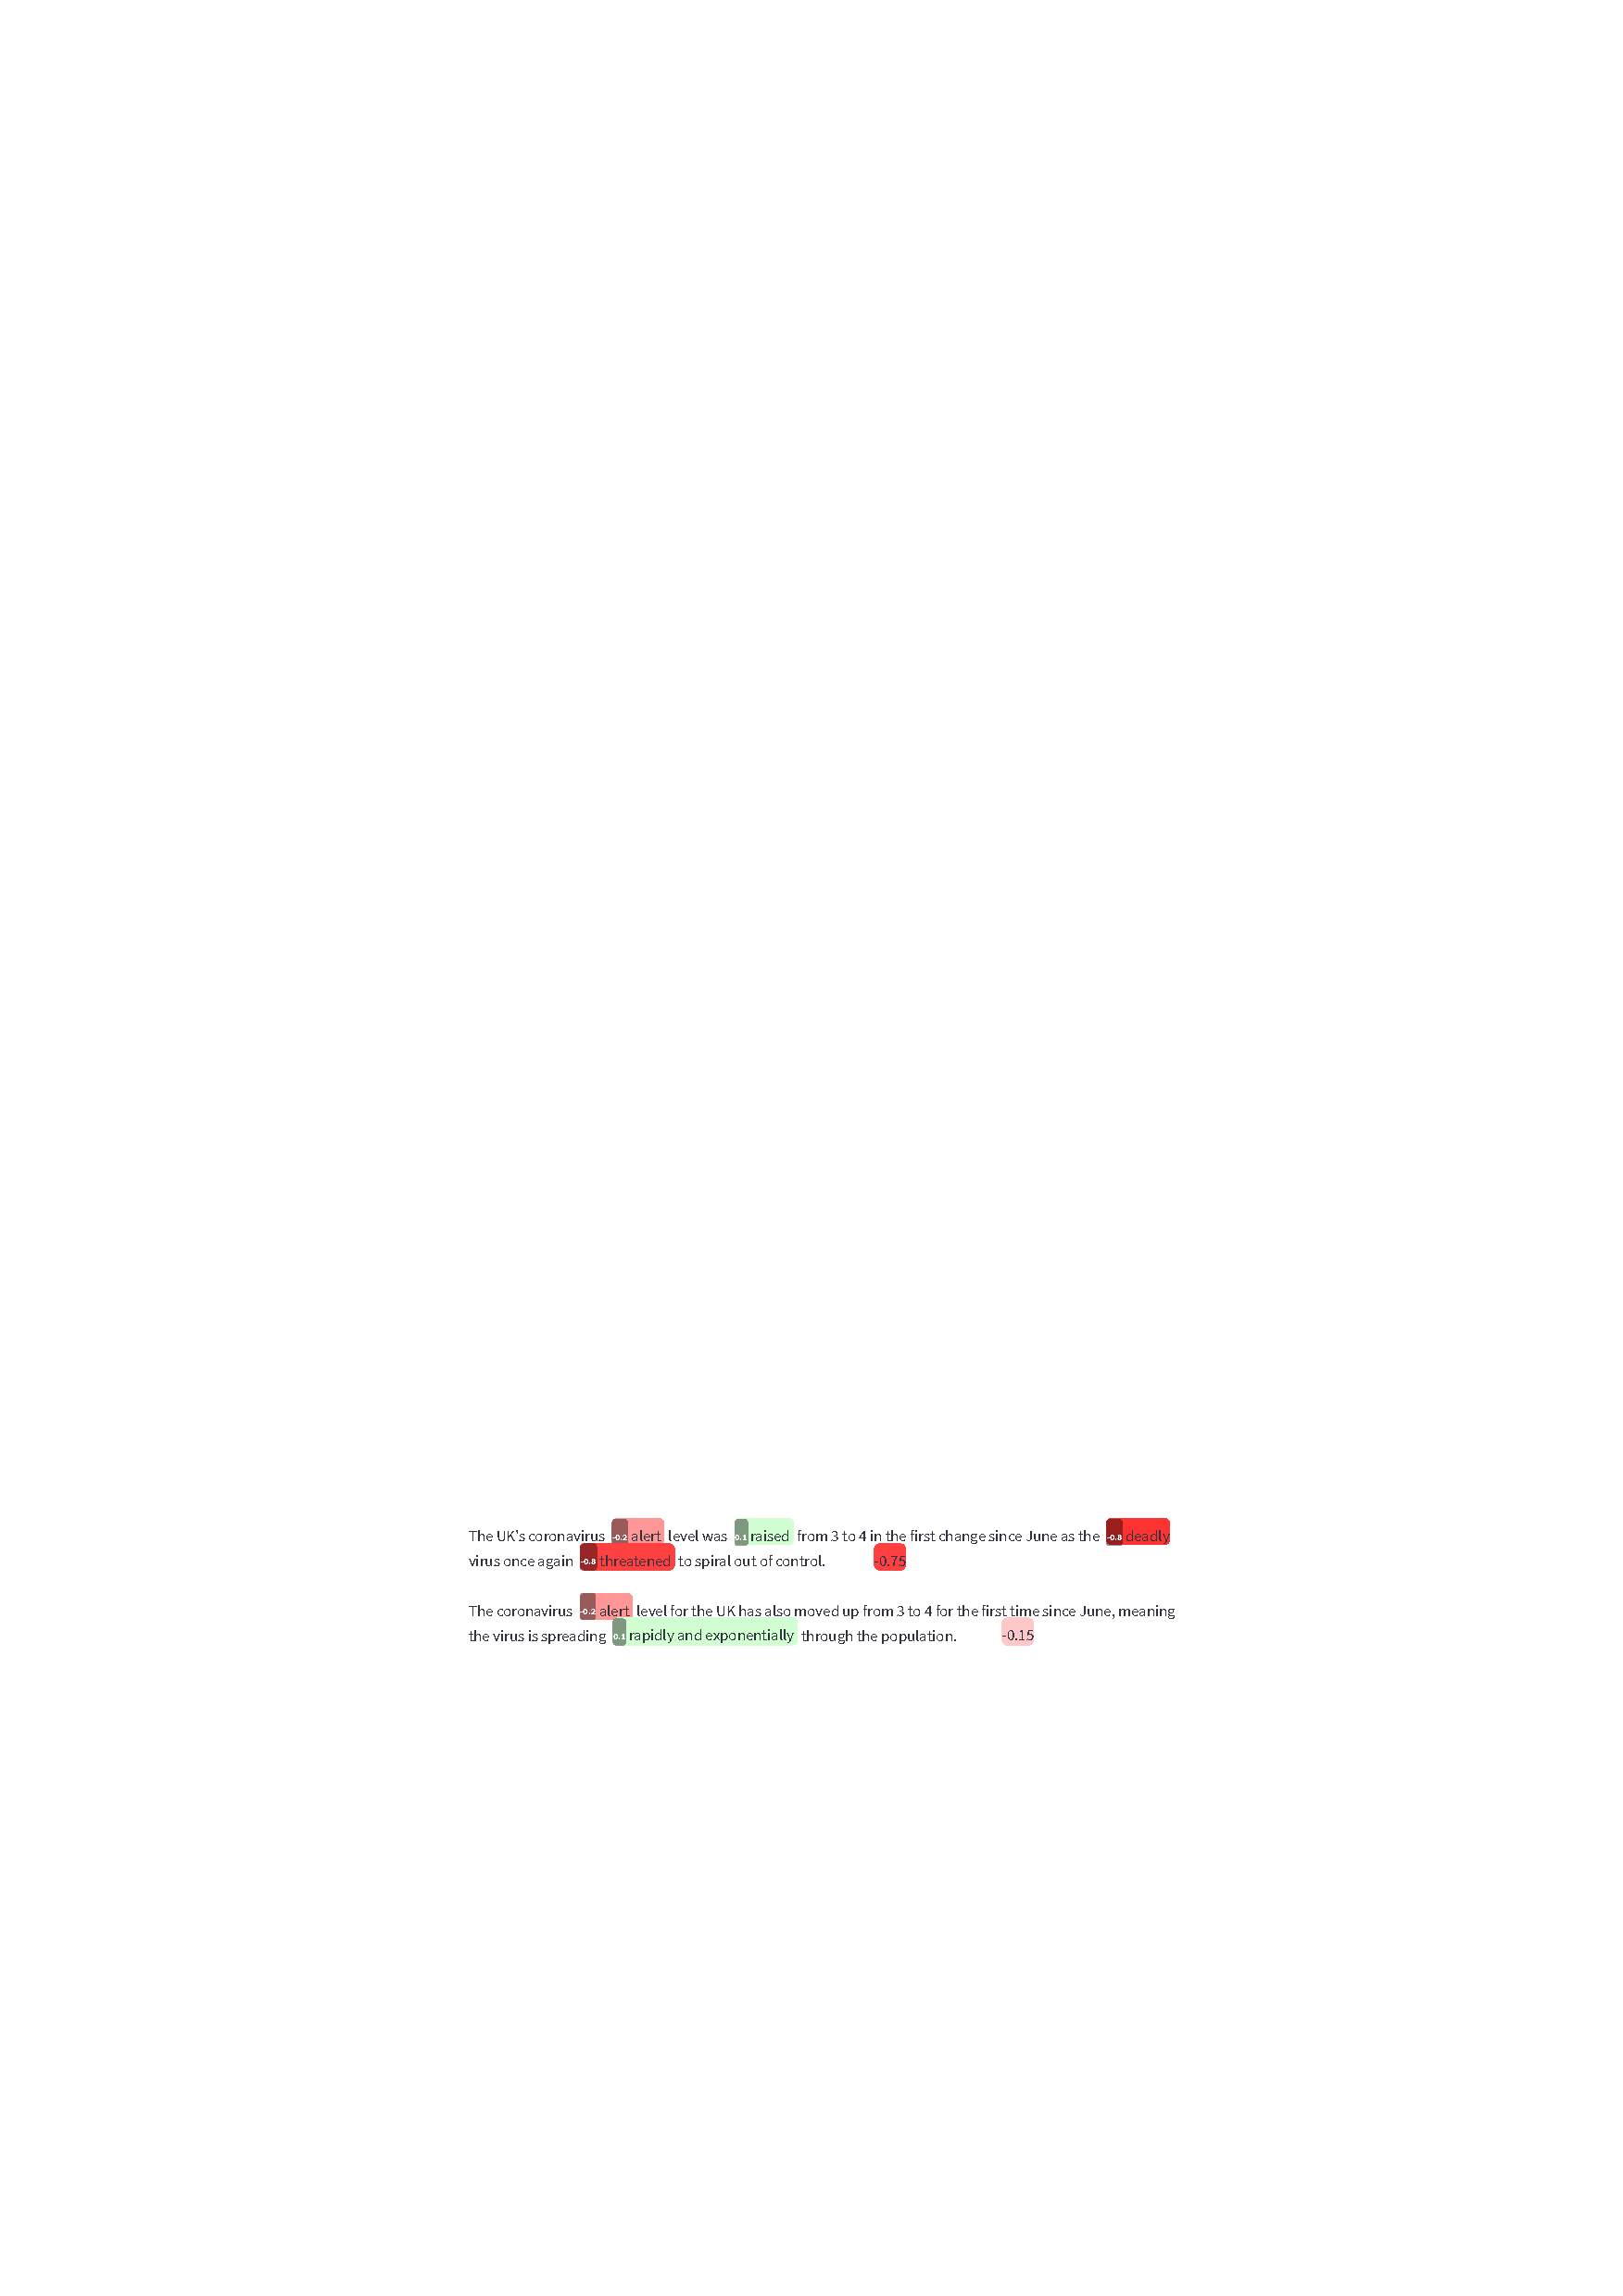
\includegraphics[width=\linewidth]{figures/updated_annotation_212_sentiment_cropped.pdf}}
    \caption{Sentence-level and word-level sentiment detection on a sentence pair.}
    \label{fig:example_sentiment}
\end{figure}

For example, let us consider Figure~\ref{fig:example_sentiment}.
The words with a coloured background are detected to carry sentiment, while the score at the end of the sentence represents the output sentiment of the whole sentence.
If we only consider the output scores at the sentence level, we just have the result that the first sentence is more negative than the second one. With only a single overall score, it is difficult to compare the single words that are responsible for the scores.
% \todoAW{You really need an example here. I don't understand why you think that a sentence-level analysis is not helpful, nor why a word-level analysis would help.}
%\todoAW{Not sure what you're getting at here. What information exactly are you hoping for at the word level? And it's not usually single words that persuade; rather, it's usually a sentence or article. So it's fine to want to identify the properties of the words that make them propagandistic, but I'd be wary of suggesting that that means you shouldn't be trying to also do a sentence- or article-level analysis.}
With the word-level scores instead, we can see the single terms responsible for the score, and compare them with what changes between the sentences (analysis from the previous chapter).
However, having a score on the sentence-level is useful to capture complex cases where no specific word is responsible but it is the context that makes a subset of words responsible for the persuasion techniques of the text (e.g. when using \texttt{Doubt} or \texttt{Repetition}).
Therefore, we need both word-level and sentence-level outputs from the analysis.
%We need to have in output the responsible words from the analysis tools, because we want to see how persuasion differs when very similar sentences exist. We can already compute which words differ, and we want to see if these words are also expressing persuasion.
% \todoAW{You've attempted a justification here, but it's very wordy and I can't follow it. An example would clarify things much more.}

In the following subsections, we illustrate the models that we are using to perform sentiment detection (Subsection~\ref{ssec:lp_techniques_sentiment}) and fine-grained propaganda detection (Subsection~\ref{ssec:lp_techniques_propaganda}).

% Then in Subsection~\ref{ssec:lp_techniques_populism_vs_propaganda} we show some work done on populism. Even though we don't have computational detection of populism, we wanted to see the relationship that it has with propaganda.\todoAW{Not sure this para is necessary}

\subsection{\statusorange Sentiment Detection}
\label{ssec:lp_techniques_sentiment}

First of all, we start with sentiment detection.
As we have seen in Chapter~\ref{chap:literature}, persuasion is very often related to an emotional response from the reader, being related to emotions~\citep{rocklage2018persuasion,petty2015emotion,desteno2004discrete} and to sentiment~\citep{gatti2014sentiment}.
% While computational approaches to detect emotions exist (usually quantified across the 5-big emotions),\todoAW{Which are? Reference? (x-ref, if you've discussed elsewhere)} the computational tools available for sentiment detection are more numerous and more common.\todoAW{than what?}
% The main difference of only using sentiment detection instead of emotions\todoAW{I don't know what difference you're trying to draw between sentiment and emotion.} is that it usually gives an output on 1 or 2 axes:\todoHA{this not a good enough reason to ditch emotion analysis altogether. 
% might be best to only talk about sentiment here, and leave the mention of emotions to the end of the chapter in the discussions section, and again in the Discussions chapter for the whole thesis.} %\todoAW{Wouldn't a 2-dimensional analysis be more fine grained than a 5-bucket "big emotion" analysis? In which case, it's an advantage of using sentiment rather than emotions.}
% valence (positive or negative) and strength (from neutral to strong). %But for an initial analysis, we deem\todoAW{How?} that sentiment is enough.
We have seen that sentiment detection gives outputs over two different axes: polarity (positive or negative) and strength (from neutral to strong).

For the reasons introduced above, we focus here on term-based analyses that
% For detecting the sentiment, we decide to use term-based analyses. % that, despite being less accurate than huge deep-learning models, \todoAW{How much less? If they're doing different tasks (word-based v. document based), how can their relative accuracy be measured?}
%\todoHA{in comparison to what?}
can provide the specific words responsible for the output.
Our main focus is to see which words are responsible for the sentiment scores, %, instead of optimizing for accuracy.\todoHA{best not to bring up accuracy at all here. not at this stage. you don’t want to tell the reader up front that your approach is not accurate enough. }
% Our main reason is to be able 
to find words that are loaded with sentiment. %If the score of sentiment is not perfect, it is not a problem.\todoHA{unclear} \todoHAinline{You are telling the reader that accuracy will be bad, and that this is ok. But unclear why it will be bad, and why this is ok. Better to leave accuracy to much later, rather that accepting low accuracy upfront}

In the next paragraphs, first we describe the chosen detection tools, then we describe how we combined them together and what they are able to extract on the considered datasets. Finally, we conclude with some findings that we discovered while applying sentiment detection to news articles. % (big variations of sentiment across the articles, correlation with quotation).
%\todoAW{If you're using OTS sentiment analysers, you don't really need to justify their lack of accuracy. Rather, you should focus on what it means for your own results, and whether the (lack of) performance of the sentiment analyser will excessively impact your work.}

\subsubsection{\statusgreen Sentiment Analysis Tools}

Being our main goal to get the words responsible for sentiment scores, we primarily focus on lexicon-based methods.
% For detection, most of the methods that we pick are lexicon-based. This happens because of our focus on getting the words responsible for the scores.
% \todoHAinline{change the order. start by explaining your needs, and justify them, then explain what you found/selected}
% Most of these tools work based on a lexicon that is combined with different scoring mechanisms (e.g., sentistrength, textblob, vader).
They are built around a lexicon where each word has a specific score, and some combination rules.
However, we do not exclude tools that work with a different, more complex approach. It is only required from them to give a score specific to the individual words. For example we also selected Stanford CoreNLP which is based on a RNN~\citep{socher2013recursive}.
%that accounts for the sequence but also for the dependency tree of the sentence.
%(in other words, discovering the combination rules autonomously).
It is not based on a lexicon, but instead on a more complex dataset linking sentiment scores to a dependency tree.
% We selected the following methods: sentistrength, textblob, vader, Stanford CoreNLP

% how we extract the word scores from lexicon
Some of the tools that we use (e.g., TextBlob described below) natively provide methods to get a list of terms that are loaded with sentiment.
Some other tools (e.g., Sentistrength, Vader below) instead only provide the total score on the sentence/document level.
However, having the lexicon provided together with the tools, we can obtain the word-level information by matching the lexicons (that provide the words + scores) with the analysed sentence.

The method to align the lexicon with the sentence is the following:
\begin{enumerate}
    \item the lexicon is loaded: the lexicon provides words (with sometimes jolly operators ``\texttt{*}" and ``\texttt{?}" to match with more than a single word) and sentiment scores;
    \item the sentence is segmented into words;
    \item the sentence words are matched with the lexicon words;
    \item the sentence words are attributed with the lexicon scores.
\end{enumerate}

% Describe each of the methods
Here we describe each of the methods used.

\paragraph{Sentistrength}
The first tool considered is Sentistrength,\footnote{\url{http://sentistrength.wlv.ac.uk/}} built around a lexicon of 2546 words (or in some cases \emph{word stems}) where each entry is annotated with a score (integer in the range $[-5;5]$) and a set of combination rules considering negations, boosters, questions.
% \todoAW{Examples?}
Figure~\ref{fig:sentistrength_example} shows an example of these sets.

% figure from https://www.researchgate.net/publication/273339197_A_Framework_for_Sentiment_Analysis_in_Persian/figures?lo=1
\begin{figure}[!htbp]
    \centering
    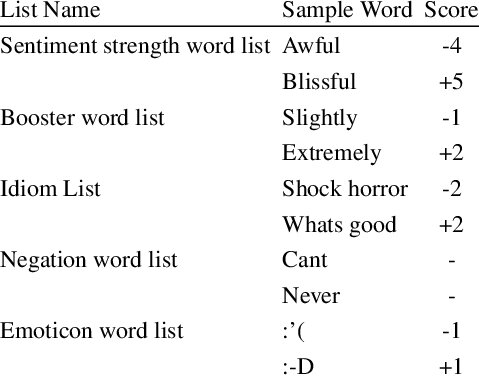
\includegraphics[width=0.5\linewidth]{figures/sentistrength_example.jpg}
    \caption{Sample words from the lexicon of Sentistrength.}
    \label{fig:sentistrength_example}
\end{figure}

The outputs given can be retrieved in different forms:
\begin{itemize}
    \item Dual score: as the name suggests, it gives two values, one for the Negative score ( -1 not negative to -5 extremely negative) and a Positive score (1 not positive to 5 extremely positive). A sentence can be both positive and negative so the two scores are independent
    \item Binary $\set{positive, negative}$
    \item ternary $\set{positive, neutral, negative}$
    \item Scale: integer value in $[-4;4]$,
\end{itemize}

However, as we said, we are interested in the single words responsible for the sores, so we use the method explained above to align the analysed sentence with the lexicon of this tool.
% to adapt the tool to output them. We achieve this by comparing the sentences with the lexicon and outputting the original scores given to them.
% \todoAW{Do we get more detail on this anywhere? Need a x-ref.}

\paragraph{Vader}
Very similarly to Sentistrength, also Vader\footnote{\url{https://github.com/cjhutto/vaderSentiment}} has a lexicon-based approach and does not natively give in the outputs the words responsible for the sentiment. Vader has been built mostly to analyse social media content, optimised for short texts.
Its lexicon is composed of 7520 words, and each entry has the raw annotations (10 annotations with integer value in $[-3;3]$) and the mean score + standard deviation.
The outputs can be read in two modalities:
\begin{enumerate}
    \item compound: where each analysed text gets assigned a single value (float) in the interval $[-1;1]$ (-1.0 negative 0 neutral 1.0 positive);
    \item separate scores: Positive, negative and neutral scores which sum to $1.0$.
\end{enumerate}

Also for Vader, to obtain the single words that are loaded with sentiment, we use the method described above to align with the lexicon.
% The advantage of this tool is that the lexicon is much larger than the one from Sentistrength.
% \todoAW{Risky comment: you can modify sentistrength with your own lexicon and then retrain it. This is pretty well established, so I don't think you can really count this as an advantage unless you can convicingly argue that you've a good reason for only considering the prebuilt models.}
% \todoAW{Did you address my earlier comment on lexicon size?}



\paragraph{TextBlob}
The next tool is TextBlob,\footnote{\url{ https://textblob.readthedocs.io/}} which instead provides already the words/parts responsible for the sentiment, whithout the need to look at the lexicon separately.
The lexicon only contains adjectives and adverbs, in total 2918. Each one of them is marked with the \emph{polarity}, \emph{subjectivity}, \emph{intensity} (for the booster words / adverbs) %\todoAW{What's a booster word? "very", for example? If so, that's an adverb, not an adjective.} 
and with the \emph{confidence}. Having these scores, the tool keeps track of the input text across two dimensions: polarity and subjectivity.
Therefore, the outputs of the analysis are the two scores of \emph{polarity}, a real value in $[-1;1]$ (-1 negative, 0 neutral, 1 positive), and \emph{subjectivity}, a real value in $[0;1]$ (0 objective, 1 subjective).

It has a relatively small lexicon, but it has the advantage of being focused on the adjectives and adverbs.
Therefore, if used in combination with other tools, it will provide more adjectives and adverbs, while the other tools will provide more nouns and verbs.
%\todoAW{Why is that an advantage? If I describe someone as a "bearded idiot" for example, then I'm intending the noun to be the main sentiment bearer rather than the adjective.}


\paragraph{Stanford CoreNLP}
Finally we consider Stanford CoreNLP, which is a tool that performs several NLP tasks, and one of them is sentiment analysis.
Differently from the previous tools presented here, this tool is based on a more elaborated approach involving a special RNN which relates to the parse tree. 
The dataset used to train this sentiment analysis model is Sentiment Treebank\footnote{\url{https://nlp.stanford.edu/sentiment/treebank.html}} which contains sentiment scores linked to dependency trees.

The outputs of the sentiment analysis module are dual. There is an overall score of sentiment to the full sentences. It also generates a SentimentTree which is a representation of how the sentiment is conveyed from the leaves (the single words) to the full sentence, following the dependency tree.
The scores in output (both total and parts of the tree) have an integer value in the interval $[0;4]$ (0 = Strong\_Negative, 1 = Weak\_Negative, 2 = Neutral, 3 = Weak\_Positive, 4 = Strong\_Positive).

% \begin{figure}[!htbp]
%     \centering
%     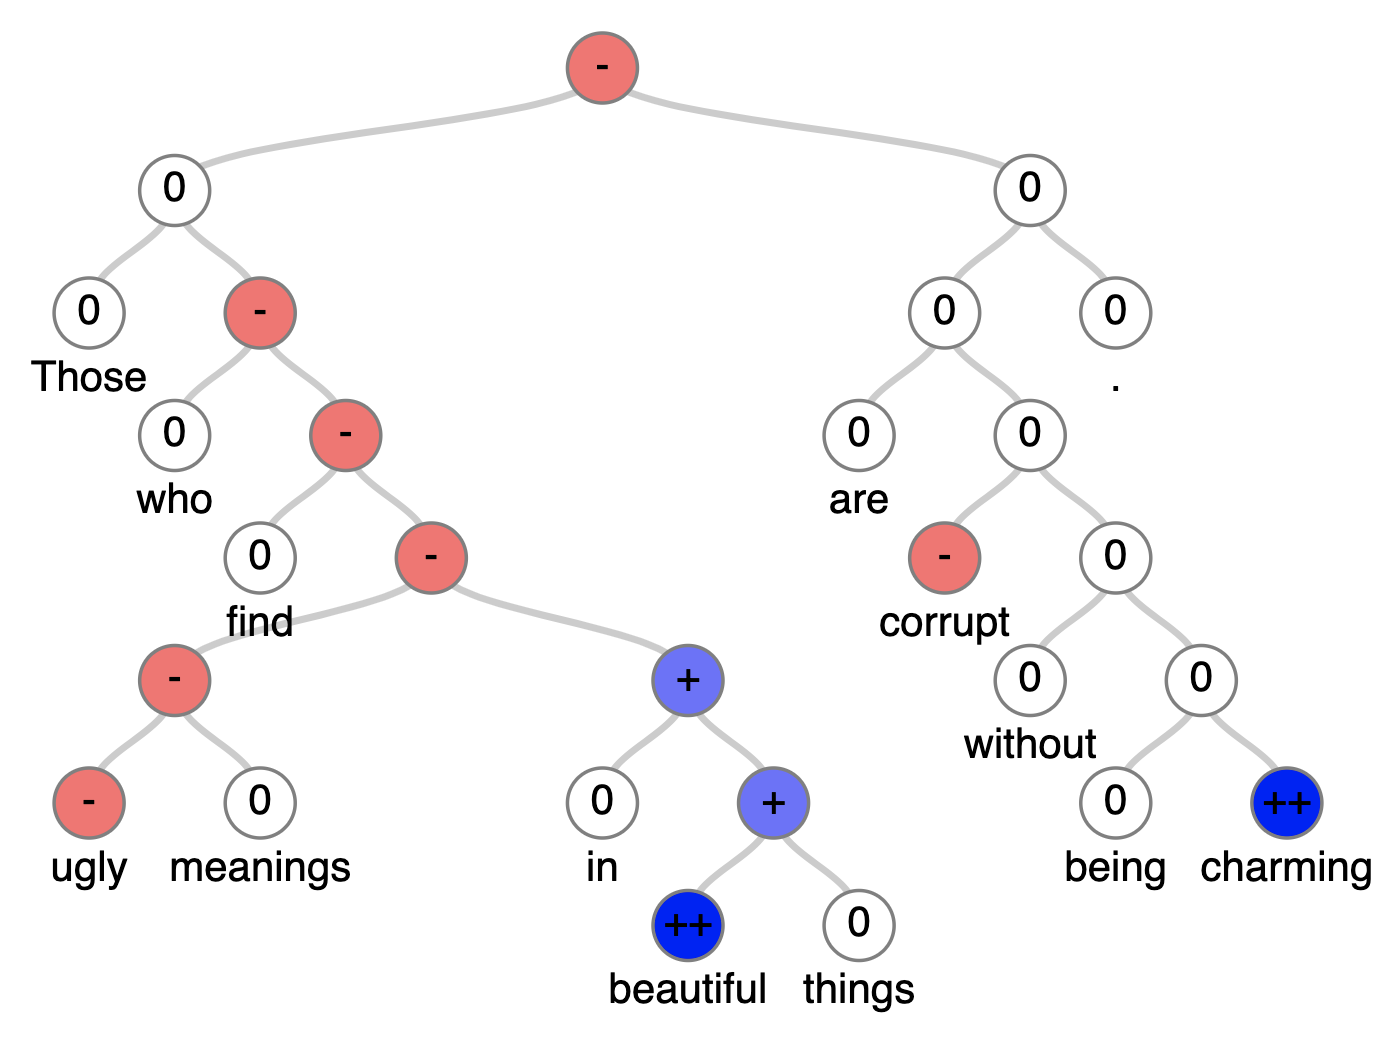
\includegraphics[width=\linewidth]{figures/parse_tree.png}
%     \caption{A SentimentTree parsed. We can extract the sentiment scores of each word.}
%     \label{fig:parse_tree_corenlp}
% \end{figure}

\begin{figure}[!htbp]
     \centering
     \begin{subfigure}[b]{0.45\textwidth}
         \centering
         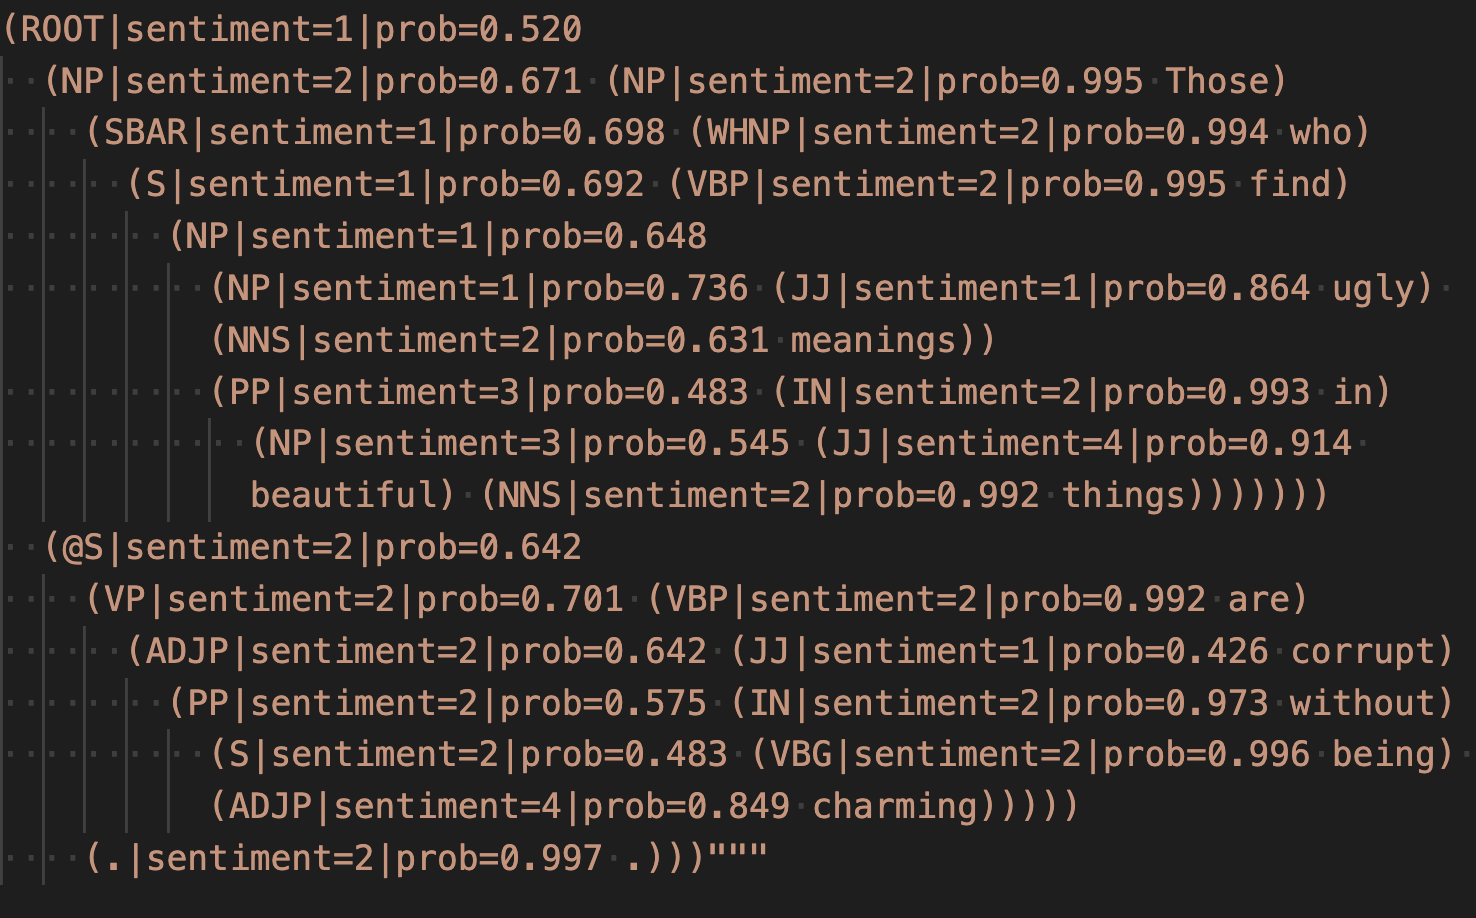
\includegraphics[width=\textwidth]{figures/sentiment_tree_2.png}
         \caption{SentimentTree generated by CoreNLP}
         \label{fig:raw_sentiment_tree}
     \end{subfigure}
     \hfill
     \begin{subfigure}[b]{0.45\textwidth}
         \centering
         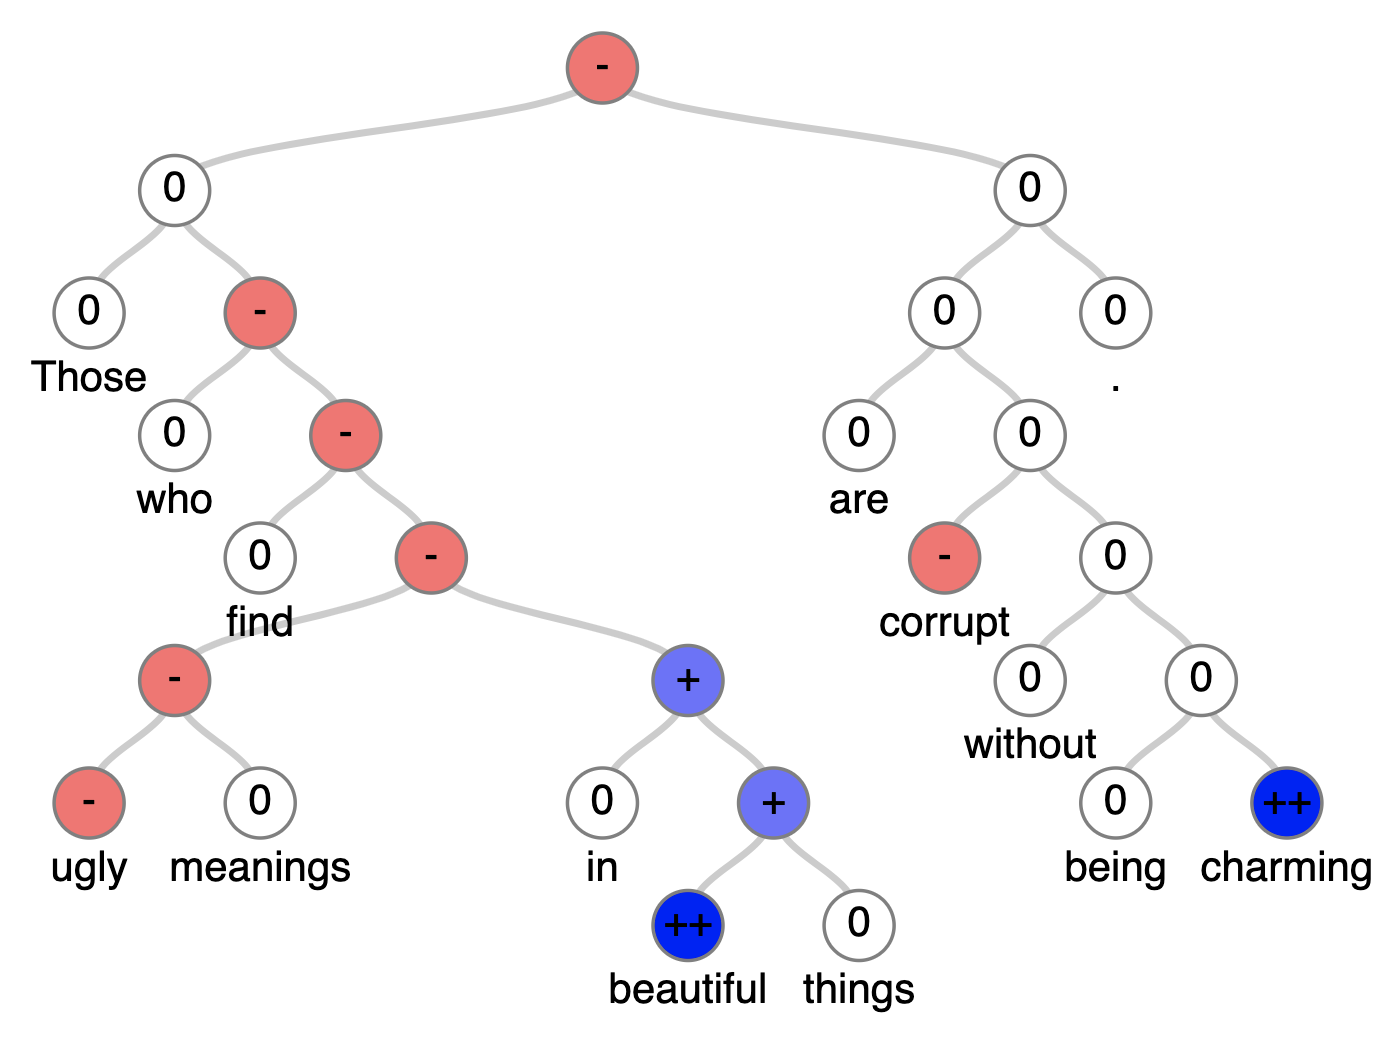
\includegraphics[width=\textwidth]{figures/parse_tree.png}
         \caption{SentimentTree parsed}
         \label{fig:parsed_sentiment_tree}
     \end{subfigure}
        \caption{Inputs and outputs of the parser for SentimentTree.}
        \label{fig:parsing_sentiment_tree}
\end{figure}

From the SentimentTree, we wrote a parser that parses its syntax and extracts the scores to the single words.\footnote{\url{https://github.com/MartinoMensio/corenlp-sentiment-tree-parser}}
Figure~\ref{fig:parsing_sentiment_tree} shows the input and outputs of this parsing. On the left, the input SentimentTree from CoreNLP. On the right, a visualisation of the parsed tree, which allows to extract the sentiment of each word.
% \todoAW{I don't think we did; writing a parser is a major undertaking.}
In this way, we are able to see the sentiment of the single words and not only the overall score for a sentence.
%\todoAW{Really needs some examples to illustrate this point.}

% \todo{
% 1. Compare outputs of the tools
% 2. Justify combination
% 3. Say how combination
% }

\subsubsection{\statusgreen Statistics over AllSides Dataset}

% How they perform separately on the dataset (justifying why all of them) and the result of combination.
In this subsection we provide some statistics about how the described approach for sentiment detection works on the AllSides dataset.

% average scores
We compare here the scores and the words provided by the different tools listed above.
To compare the values, given that each tool has its own scale, we first normalise all of them to the same interval of $[-1;1]$.
To normalise the scales, we consider two main axes: polarity (used by all of the tools) and strength (provided by SentiStrength, and subjectivity by TextBlob). We map the numerical intervals from the corresponding $[min;max]$ to $[-1;1]$ by means of a linear transformation. The categorical values, instead, are mapped by firstly sorting the output labels from negative to positive, then converting to increasing numerical values (e.g., for 4 labels, $\set{1,2,3,4}$) and then applying the linear transformation as in the other case.

% - Unified scores by each tool (polarity and strength)
% For the output scores, we consider the unified scores discussed previously. 


\begin{figure}[!htbp]
     \centering
     \begin{subfigure}[b]{\textwidth}
         \centering
         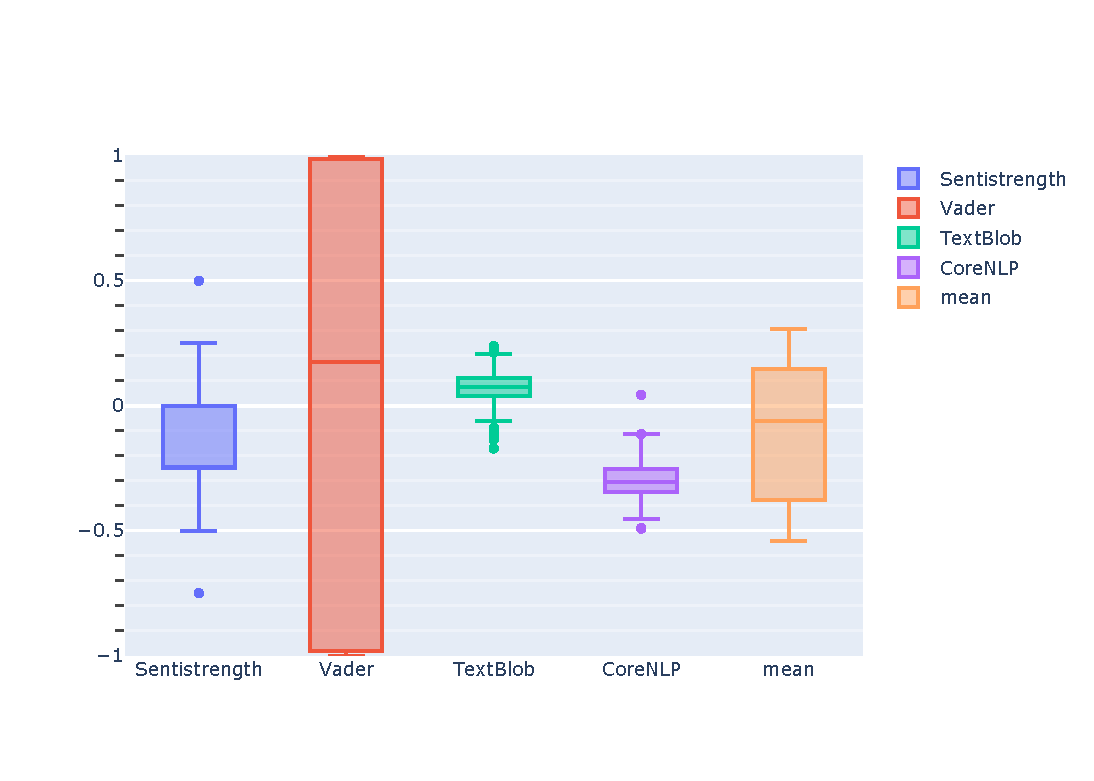
\includegraphics[trim={0 1.5cm 0 2cm},clip,width=\textwidth]{figures/sentiment_polarity_comparison.pdf}
         \caption{Sentiment polarity}
         \label{fig:sentiment_polarity_comparison}
     \end{subfigure}
     % \hfill
     \begin{subfigure}[b]{\textwidth}
         \centering
         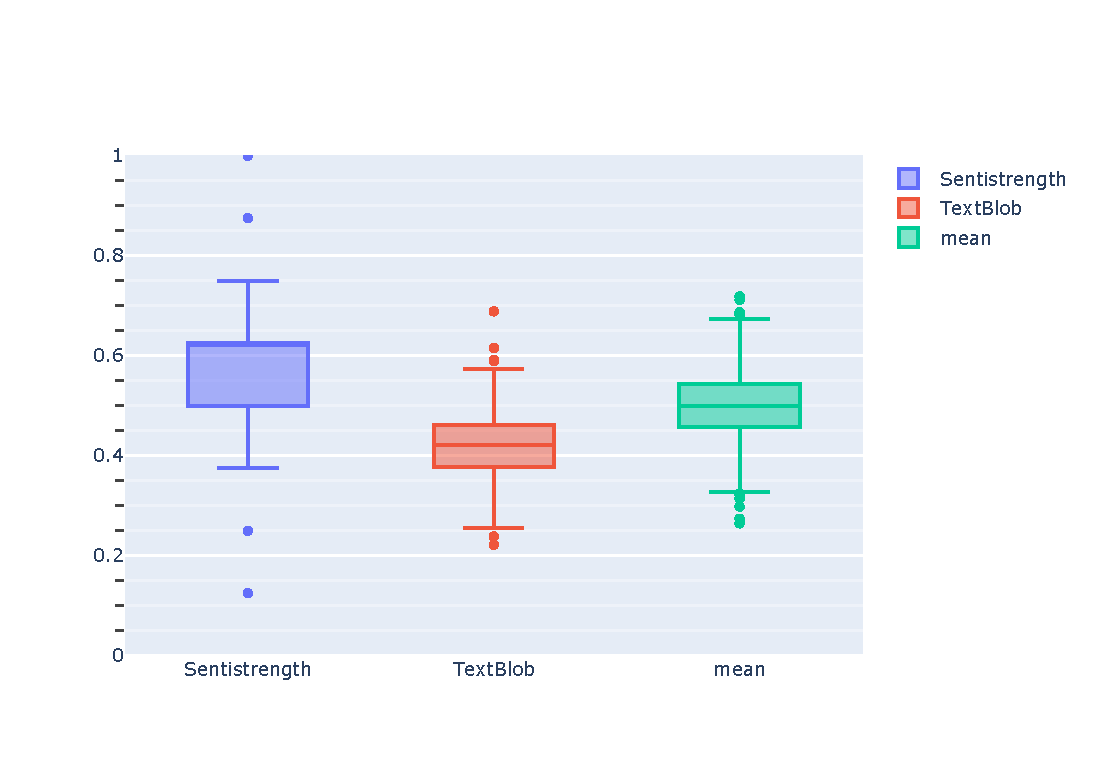
\includegraphics[trim={0 1.5cm 0 2cm},clip,width=\textwidth]{figures/sentiment_strength_comparison.pdf}
         \caption{Sentiment strength}
         \label{fig:sentiment_strength_comparison}
     \end{subfigure}
        \caption{Sentiment polarity and strength provided by different tools.}
        \label{fig:sentiment_axes_comparison}
\end{figure}

For each article, we produce the outputs using each tool, and we then aggregate over the whole dataset.
Figure~\ref{fig:sentiment_axes_comparison} shows the average values across the two main axes considered (polarity and strength).
The plot shows boxplots that represent the median (line in the middle of the box), first and third quartile (colored box boundaries) for the considered tools (four for polarity, two for strength) and for the arithmetic mean.
We can see that, even being normalised to the same interval, these tools provide different distributions.

% - polarity
Starting from the polarity values, that describe how positive or negative is the sentiment, we have some tools that have values more extreme than others.
Vader, for example, has values that are very spread out.
For example, the values of Vader reach very often the maximum and minimum (first and third quartile).
TextBlob and CoreNLP instead have a much smaller range, but with a different mean. CoreNLP provides generally more negative results, while TextBlob more positive ones.

% - strength
For the sentiment strength instead, we only have two of the four considered tools that provide values.
The distributions show differences across tools, with Sentistrength providing the higher values.


% % - Correlation between tools
% Then we proceeded to study the correlation between the outputs of the different tools.
% The most correlated are ???
% Instead ??? provides results quite unrelated to the others.

\begin{figure}
    \centering
    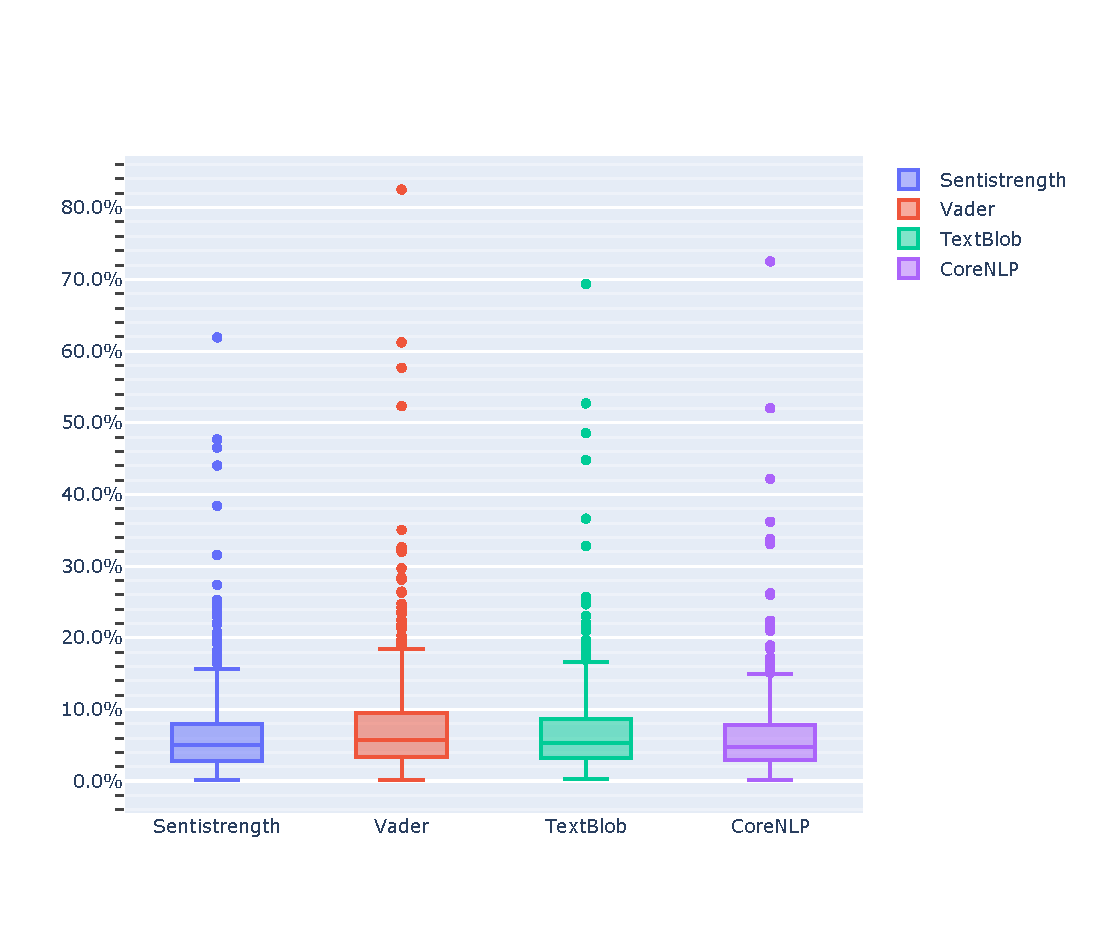
\includegraphics[trim={0 1.5cm 0 2cm},clip,width=\textwidth]{figures/sentiment_words_comparison.pdf}
    \caption{Percentage of sentiment words provided by different tools.}
    \label{fig:sentiment_words_comparison}
\end{figure}

% Words:
% - percentage of words detected by each tool
For the analysis of the word-level instead, we computed the percentages overall the whole datasets of the words detected by each tool.
Figure~\ref{fig:sentiment_words_comparison} shows the word-based percentage of sentiment. To obtain this value, we count the terms that are detected as carrying sentiment for each article.
For some tools, these are provided natively, while for others we use the lexicon alignment described previously.

We can see from this figure that each tool detects a quite high number of words as related to sentiment ($5-8\%$), and for some outliers we reach values above $50\%$.
% - percentage of words detected by combination

% % - term analysis: most frequent words positive/negative
% We also perform a term analysis to see which words are the most frequent positive/negative. Figure~\ref{TODO} shows that ???

% % Group by News source:
% We also break down the analysis to the individual news sources.
% % - sources with highest/lowest/strongest
% We find that the sources with the most positive sentiment are ??? while the ones with most negative sentiment are ???.
% Instead on the axis of strength, the news sources that have strongest sentiment are ???
% % - most frequent sentiment words for the most frequent sources

% \todo{figure by news source}

Overall, we see that using these tools introduces one main limitation: false positive words. Many times by inspecting the results, we see that words that should not be sentiment-related instead are annotated as such, as also Figure~\ref{fig:sentiment_words_comparison} denotes.
%Also by looking the overall percentages, we can see that they are relatively quite high.
% How am I compensating for it?
We already removed the outputs from some other libraries because they were providing even more wrong results, but this remains a main problem.

% Combined results? Or stop

\subsubsection{\statusgreen Combination of the Tools}

% \todoAWinline{So from the previous section, I don't really get a sense of the practical differences between the approaches, as you haven't given a running example that would let me see what the difference between the systems is. Also, you don't seem to have discussed what scope there is for adjusting the lexicons for each system, or what difference that might make to the final analysis.}
% \todoHAinline{deciding to combine upfront is not very good. Better way is to use them individually, then combine. This way you scientifically demonstrate value of each approach.}
% Why combine
From this list of tools, we decided to combine them together in order to increase the accuracy of the sentiment recognition. %\todoAW{I think you mean that you wanted to improve the accuracy of the sentiment recognition.}
% As each one of them has different
%\todoHA{what if they contradict each others?} 
% lexicons covering different groups of words (e.g., TextBlob only adjectives),
%and given that they do not overlap totally,
% \todoHA{avoid such vague language. This is also not supported by any data. Why not?}
For the sentiment score, we opted to use an arithmetic mean to provide more stable results.
In case of failure of one of the tools, if we consider the average we have a safer score to provide.

Instead, for the word-level detection, we have the problem of too many words being produced by each of the tools.
Therefore, we decide to use a combination rule that annotates a word when at least two of the tools detect it as carrying sentiment.
In this way, we reduce the amount of false positives.
% As each tool provides different words in output
% the combined lexicon (not correct word, because CoreNLP does not use one) / detection power can be much larger than just considering one of them.
% \todoAW{proof?}

% How combined all of them
We therefore combine the tools in the following way:
\begin{enumerate}
    \item running the tools in parallel;
    \item collecting the results;
    \item numerical scores: uniforming the scales (each tool has a different one) and averaging the single scores out;
    \item sentiment words: doing the union of the words that are recognised by at least two tools, and for each word we compute the average score (again by uniforming the values first).
\end{enumerate}
% we run them in parallel for each input text, and then we collect the results.
% We consider two types of outputs: the score(s) given to the text, and the words responsible for the score.

% For the score, uniforming the scales and doing the average. Ranges --> conversion --> average

% For the words, we take the union of the words outputted from each tool. Each word can then have a positive/negative score so we also merge them,.
% If one word is given back by just one tool, then the score is given by the tool (uniforming again the score as above). Instead if the word is given back by multiple tools, we consider it only once and we average the uniformed scores.

Even if we average and combine the results, we keep the original outputs for each tool in order to backtrack the results and see where the problems come from.


% \todoAW{Would it have made more sense to combine the lexicons from the different systems and then used them to augment one of the existing models (eg. SentiStrength)? Even if not, you should be prepared to answer that question in your viva.}


% \subsubsection{\statusorange Sentiment variation along articles}

% \todomargin{MM: Maybe this subsection is not important, and drifts away from the main focus of this chapter}

% With this setup of the tools, we moved to inspect the articles more closely. We want to see how the sentiment changes from the beginning to the end of the articles.\todoHA{why? what is the value of knowing this?} %and if it is linked to any other external factors.\todoHA{like what?}\todoAW{Such as the reader? Very vague!}
% % We then experimented with the selected libraries to see how they could analyse the sentences in news articles. 
% We started by observing how the sentiment scores vary across one article at a time, when we consider the sentences of the articles.\todoAW{Earlier, you were arguing that you were concerned about word-level sentiment rather than the sentence or article level}
% For each sentence, we compute the sentiment scores and then we compare how the tone varies across a single article at a time.\todoHA{changes how? and what change would tell us? remember that reader won't know why you are doing something unless you make that clear}
% For example, fluctuating between subjective and objective tones.

% Figure~\ref{fig:sentiment_across_one_article} shows how the detected sentiment changes a lot across an article.
% \todo{which article is it? Why this one?}
% Some sentences appear to be very neutral, and some instead are very subjective/intense. And we want to understand why and if this is only a glitch of the sentiment detection libraries.

% \begin{figure}[!htbp]
%     \centering
%     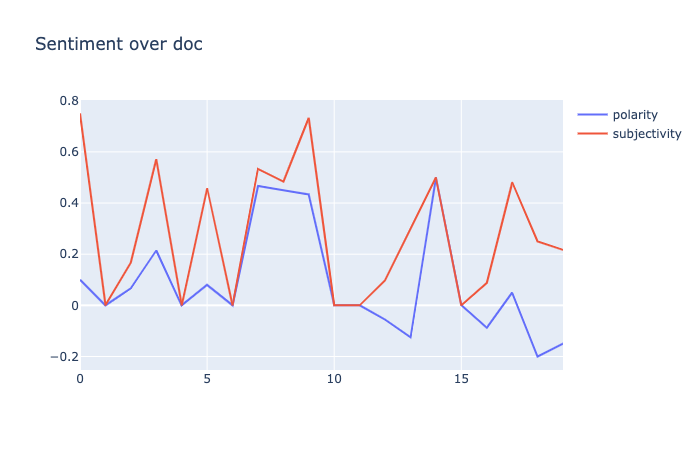
\includegraphics[width=\linewidth]{figures/sentiment_across_article.png}
%     \caption{Sentiment along a single article. Each point on the x axis is a different sentence, while vertically on the y axis several scores are plotted.}
%     \label{fig:sentiment_across_one_article}
% \end{figure}
% \todoAW{I don't understand this. Why aren't the axes labelled? What does the title mean? And where is the graph described and interpreted in the text?}
% \todo{Fig~\ref{fig:sentiment_across_one_article} coming from which libraries?}

% % \subsubsection{Sentiment is correlated to quotation}
% By looking closely at several articles where this oscillation occurs, we noticed that this duality of tones\todoHA{clarity} in the articles is mostly correlated to direct/indirect reporting. 
% Our hypothesis is that when the articles give space to some interviewee (quoted)\todoHA{shouldn't this be part of the evaluation? why mentioned here?} the sentiment libraries detects intense and subjective words/scores. Instead, when the reporter is narrating, the tone is quieter and more neutral.
% \todoHAinline{you need examples throughout}

% To study this correlation on large scale on our dataset, we tested our hypothesis by considering on one side the sentiment libraries, and on the other side a model for quotation detection~\citep{scheible2016model}.\footnote{\url{https://github.com/christianscheible/qsample}}

% For each sentence, we computed both sentiment score and the quotation percentage (defined as number of words inside a quotation divided by total number of words).
% Figure~\ref{fig:sentiment_vs_quotation} shows for the same example article, how the two measures are moving together.

% \begin{figure}[!htbp]
%     \centering
%     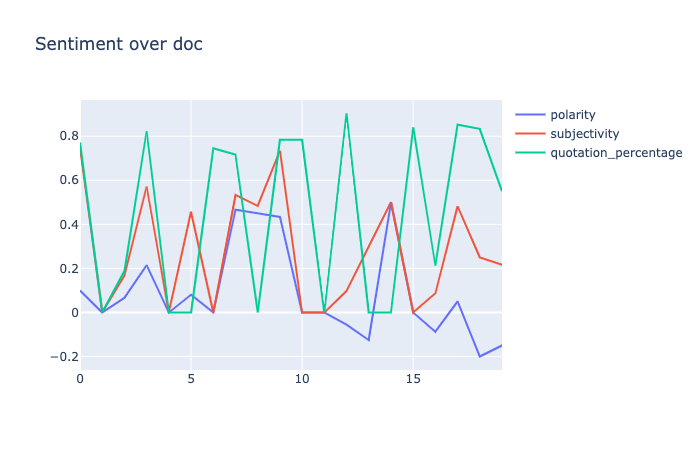
\includegraphics[width=\linewidth]{figures/sentiment_vs_quotation.png}
%     \caption{Sentiment VS quotation}
%     \label{fig:sentiment_vs_quotation}
% \end{figure}
% \todoHA{This is too crude. Think of a more precise way of measuring such correlations}

% \todo{Compute correlation across all the dataset. Quantify. Then support with some figures}

% Findings of this experiment

% Finding 1:
% Subjectivity and quotations: quotations increase subjectivity of articles, are the most subjective parts

% Finding 2 (shown in previous subsection): the results of lexicon-based sentiment detection are not very great, and they are prone to many errors.


% The conclusion is that when we consider the output scores of the sentiment analysis of sentences, the results may have a bias whether they are analysing a sentence with quotation, showing higher subjectivity and more sentiment, with respect to sentences without quotations.

\subsection{\statusgreen Fine-grained Propaganda Analysis}
\label{ssec:lp_techniques_propaganda}

As a second group of persuasion techniques, we consider \gls{propaganda}.

As we have seen in Chapter~\ref{chap:literature}, propaganda is a form of persuasion that is characterised by its goal to indoctrinate population towards an individual or a particular agenda~\citep{bernays}.
It manifests through several techniques that have been studied in the literature~\citep{torok2015symbiotic}. Each technique has its own peculiarities.

For detecting propaganda, we want an approach that gives us not only a binary label (propaganda vs non-propaganda), but we want to have an insight about which specific techniques have been used.
Knowing which techniques have been used helps us to have a more distinctive persuasion profile of the articles analysed.

Our main goal in this chapter is to describe the differences between multiple versions of the same detail, and if we have more dimensions, it is better.
For this reason, we need to have fine-grained detection of propaganda, that produces as output the specific techniques used and which words are responsible for it.
Taking from the literature described in~\ref{sec:lit_propaganda}, we consider the recent work of~\cite{da2019fine} as it is able to provide fine-grained detection. This method uses a neural network to annotate text articles and to see which words belong to specific propaganda techniques (Figure~\ref{fig:propaganda_example_1}).
The model is a sequence model based on BERT. It is based on the PTC dataset that is part of the same paper. This dataset contains articles annotated at the span level (specific words are highlighted and assigned to a specific technique). The model then learns to reproduce these annotations by looking at words in their context (sequence model).

The classification is performed on the word level, additionally using the left and right context of the text. Each word is classified as being one of 18 different techniques or none of them.
We use this detection algorithm off the shelf,\footnote{\url{https://github.com/qcri/PropagandaTechniquesAnalysisBERT}} only wrapping the code in a client-friendly environment to simplify the integration in our processing pipeline.\footnote{\url{https://github.com/MartinoMensio/PropagandaTechniquesAnalysisBERT}}


\subsubsection{\statusgreen Statistics over AllSides Dataset}
\label{ssec:lp_techniques_propaganda_stats}

We present here an analysis of how this model works on the dataset that we used mostly in this chapter.
% The dataset chosen for this are AllSides and All-the-News
The dataset, presented in Section~\ref{sec:lp_datasets}, is AllSides.

The processing pipeline that we use consists of the following steps:

\begin{enumerate}
    \item Load the text of the articles from the dataset.
    \item Use the model for fine-grained analysis of propaganda techniques: this produces a set of annotated spans in the document, highlighting the words that are detected as containing one of the propaganda techniques, together with the labels of the techniques.
    \item Compute word-level percentages of each technique for each article: we define this metric as the total number of words belonging to each technique divided by the total number of words in the article.
    \item Accumulate the frequencies of each word that is detected as containing any propaganda technique.
    \item Compute the TF-IDF of the propaganda terms counted in the previous step.
\end{enumerate}


% Stats: 
% define metrics for quantities: definition of word-based percentage, overall word-based percentage of propaganda (any techniques), technique specific percentages.
% Then present metric values for quantities.

Across the dataset, we have that on average, $5\%$ of the words are detected as being part of any of the 18 propaganda techniques considered.
The standard deviation is $4\%$, and the maximum value of $56\%$ is caused by an article that is just two sentences long. Except a few outliers caused by partial articles or errors in the scraping, the values are in an acceptable range, as the standard deviation confirms.
% https://www.nytimes.com/2019/08/06/books/toni-morrison-dead.html

% Overall word-based percentage of propaganda
% count    36274.000000
% mean         0.054099
% std          0.041590
% min          0.000000
% 25%          0.023761
% 50%          0.044807
% 75%          0.074553
% max          0.566957

\begin{figure}[!htbp]
    \centering
    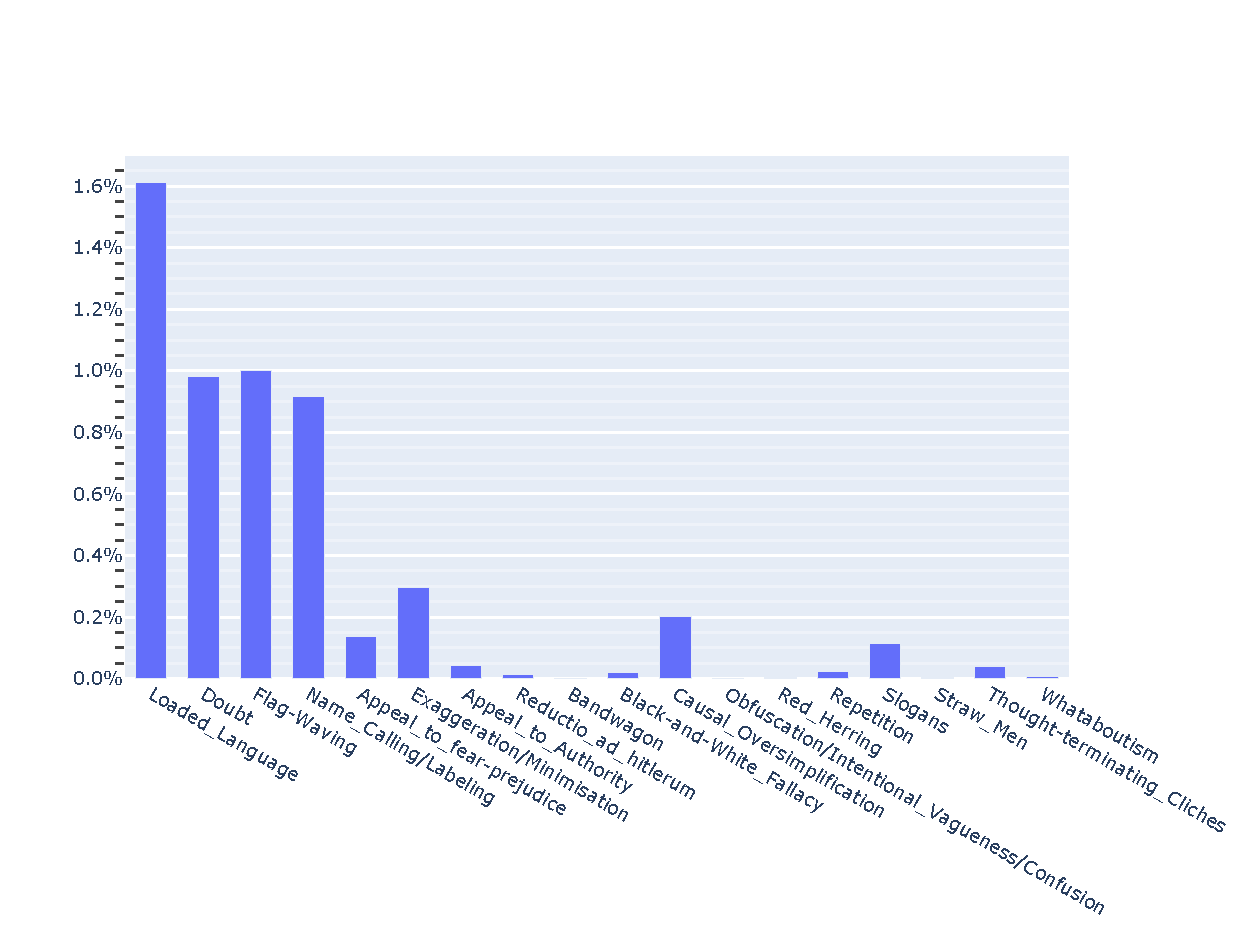
\includegraphics[width=\linewidth]{figures/prop_tech_detail_baly.pdf}
    \caption{Word-based percentage of propaganda techniques in the AllSides dataset.}
    \label{fig:prop_tech_detail_baly}
\end{figure}

We then break down the statistics to the single techniques, and we can see in Figure~\ref{fig:prop_tech_detail_baly} that several techniques are detected across the dataset.
the most frequent one is \texttt{Loaded\_Language}, which appears on $1.6\%$ of the words.
Successively, we also have other techniques that appear quite frequently (close to $1\%$, such as \texttt{Doubt}, \texttt{Flag-Waving}, \texttt{Name\_Calling}/\texttt{Labeling}. Some techniques instead are hardly ever detected, such as \texttt{Bandwagon}, \texttt{Obfuscation}, \texttt{Red\_Herring} and \texttt{Straw\_Men}.


% Term analysis define: most frequent across techniques, technique-specific terms
% Term analysis values.


% % criticism
% From its publication paper~\cite{da2019fine}, we can see in table 6 and 7 that this model has been evaluated in two ways:\todoAW{Did you attempt to reproduce this evaluation?}

% \begin{itemize}
%     \item sentence-level: binary classification, whether the sentence contains propaganda or not. For this task the reported F1 is around $60\%$\todoHA{reported dataset? clarify}
%     \item span-level (full task): whether the corrects words\todoHA{?} have been identified with the correct technique or not, so accounting both for position/boundaries and for the label. For this task the reported F1 is slightly above $22.5\%$
% \end{itemize}

% These statistics make us aware that, even though this model is the currrent State of the Art, its ability to recognise the proper techniques of propaganda are quite low overall.
% Therefore we need to take with a grain of salt the outputs coming from this model.\todoAW{Too informal. What does "tak[ing something] with a grain of salt" mean in practical terms?}

% \todoHAinline{leave self-criticism to later. also, reported \% here are only indicators since other data is different to yours}



% \subsection{\statusorange Propaganda vs Populism}
% \label{ssec:lp_techniques_populism_vs_propaganda}

% \todomargin{MM: maybe move to an appendix? Not really linked to the rest of the thesis}

% % from "Propaganda datasets unbalanced?"
% % What
% In this section, we experiment with another concept from the literature that is shown to be close to persuasion and propaganda: \gls{populism}~\citep{tumber2021routledge,pasquino2008populism}.\todoHA{Not mentioned in intro. Why not?}
% We want to understand: what is the substantial difference between populism and propaganda? Can these two phenomena be related?
% This question arises purely from a logistical point of view: we have automated methods for detecting propaganda, but we do not have tools to detect populism. Therefore, if we can prove that populism and propaganda are actually correlated, then it becomes not important for us to be able to detect something that is very much correlated to something else that we already detect.

% % concepts
% On the conceptual level, propaganda and populism are two separate concepts. The first describes more the persuasion mean used to push for an agenda, while the second one is usually used more together with the actor that wants to push the agenda. Populism is ``a type of politics that claims to represent the opinions and wishes of ordinary people".\footnote{\url{https://www.oxfordlearnersdictionaries.com/definition/english/populism}}
% And to be on the side of ordinary people, it uses propaganda as a mean. So a populistic \emph{actor} uses propaganda \emph{techniques}. Conceptually, they are related.

% \todoHAinline{ok, but what would detecting populism give you? Why is this of value?}

% \todoHAinline{I would start by: 1. explaining value of detecting populism. 2. detecting it and evaluating that, then 3. see if correlated with propaganda}

% % practically/computationally
% On the computational/detection side, we want to see if this relationship between populism and propaganda stands.
% So to evaluate it, we have computational approaches for propaganda detection, but not for populism detection.
% A solution to this problem, is to use a dataset where we have the ground truth for the populism, which will be run through the propaganda detection pipeline. Then we will compute the correlation between the two, and we can establish whether this relationship is proven. The advantage of using directly the ground truth for one of the two phenomena (populism) is that we can only have errors for the propaganda detection.\todoHA{unclear} Instead, if we were to compare two predictions, the errors could be on both sides.

% % dataset used
% For this experiment, after looking at the available datasets for populism, we selected the one from~\citet{hawkins2019global} because it is quite balanced in terms of the political orientation of the actors annotated (liberal vs conservative).\todoAW{It strikes me here that this is a very US-centric interpretation of the political landscape. Do you consider whether the make up of the dataset poses any threats to validity?}
% It contains 1240 political speeches, from several countries and languages
% For each one of them there are four annotators that give a numerical score of populism in the range $[0;2]$ where $0$ means non-populistic and $2$ means very populistic. The single annotations are already averaged out.
% So from the 4961 raw rows, by deduplicating (4 annotations for each speech) we have 1240 speeches, out of which 265 are in English (then down in the rankings, 304 in Spanish and 148 in Portuguese).

% % These 265 speeches all have a leaning classification (we will see more about leanings in the next chapter): 36 left, 37 center, 84 right, 106 NA. We use this information in order to check whether the results that we get are general across the political spectrum.
% % --> moved to chapter 5


% % Dataset found: populism in political speeches %https://dataverse.harvard.edu/dataset.xhtml?persistentId=doi:10.7910/DVN/LFTQEZ&version=2.0 
% % Each annotator (4 for each speech) gave a score between 0 (non-populistic) to 2 (very populistic)
% % 4961 rows 
% % 1240 deduped (352 left, 256 center, 469 right, 652 NA)
% % Languages: 265 en (304 es, 148 pt, …),
% % Leaning of the english ones: (36 left, 37 center, 84 right, 106 NA)



% % Goals:
% With this dataset, as we described, we want to compute the 
% correlation between propaganda and populism. So we take each speech in the corpus and we proceed to compute the Spearman's correlation~\citep{spearman1910correlation} between the  populism averaged out between the annotators and different propaganda metrics: total word-based percentage of propaganda, and word-based percentage of each of the propaganda techniques. 


% % results
% The Spearman's correlation between the populism and the total word-based percentage (all techniques together) is $0.1694$. This value is quite low. So it seems that they are quite unrelated.\todoAW{This feels to me like the sort of investigation and analysis which forms the bedrock of your research. So I think you need to set it out more formally so that it feels like less of an aside.}

% \begin{figure}[!htbp]
%     \centering
%     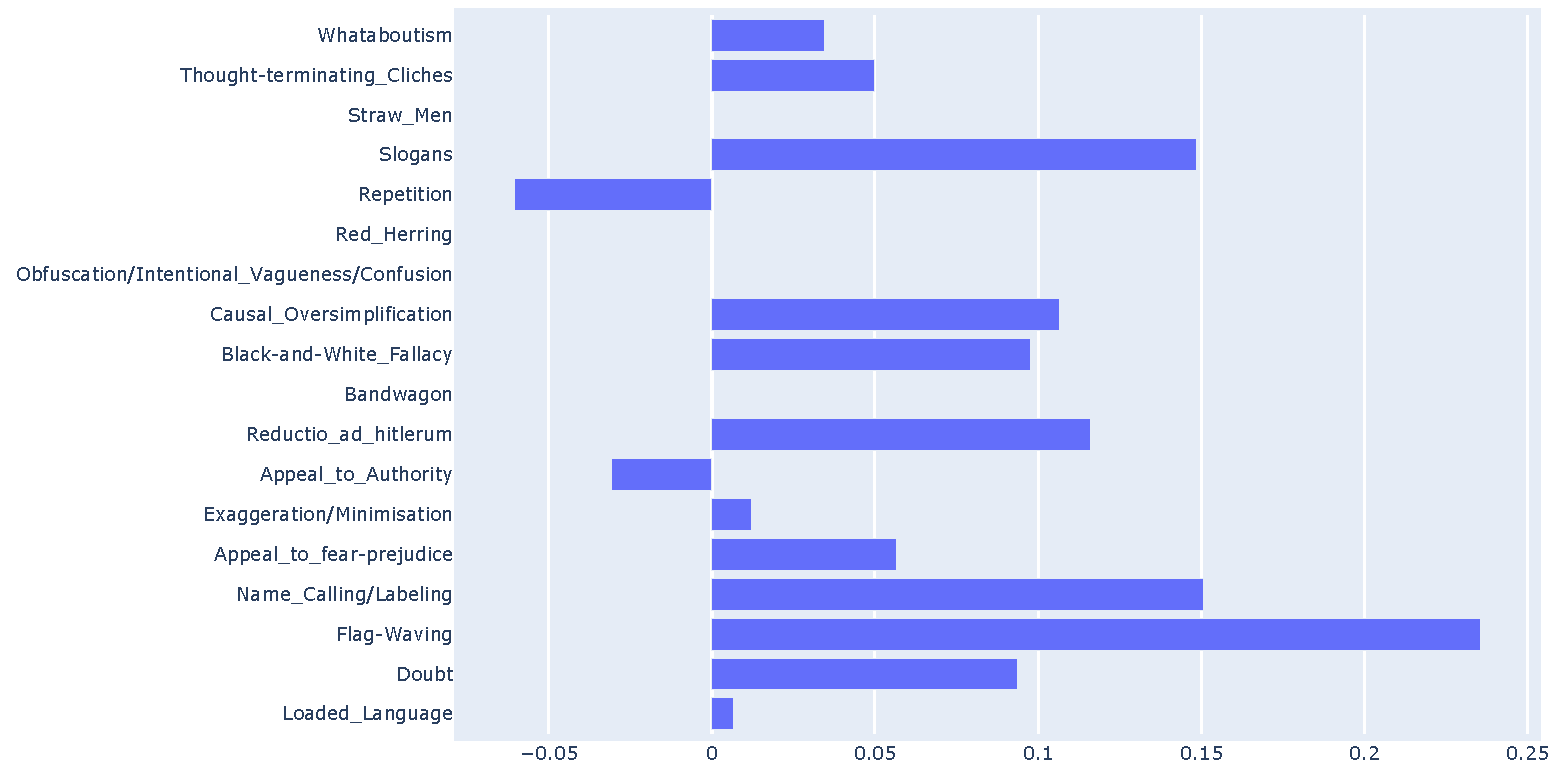
\includegraphics[width=\linewidth]{figures/populism_propaganda_correlation.pdf}
%     \caption{Spearman's correlation between populism and each propaganda technique}
%     \label{fig:populism_propaganda_correlation}
% \end{figure}

% By breaking it down to the correlation of populism to each propaganda technique, we can see in Figure~\ref{fig:populism_propaganda_correlation} that the strongest correlation is found with \texttt{Flag-waving}, \texttt{Name\_Calling/Labeling} and \texttt{Slogans}. Some of the techniques have very low correlation. It is interesting to notice that two techniques have slightly negative correlation (\texttt{Repetition} and \texttt{Appeal\_to\_Authority}), so this means that they are used by less populistic speeches.


% % L/R evaluation:
% % Assumption: propaganda correlates to populism similarly in L/C/R
% % Result total: 0.225 Left, 0.005 Center, 0.374 Right → Why? Is it a matter of quantity of populism/propaganda?
% % Populism average:  [0.1259, 0.0729, 0.2712]
% % Propaganda average: [0.0165, 0.0271, 0.0432]
% % Ratio: [0.1317, 0.3717, 0.1593] → populism over propaganda ratio is a bit bigger on the right (21\% more), but the correlation Right is bigger than the left at 66\%. So it is less likely that this is just a matter of quantity. On the Right, propaganda and populism are strongly linked

% % findings
% Propaganda and populism are correlated, but not too strongly.\todoAW{?}
% The fact that some of the techniques are correlated to populism is a good sign,\todoHA{why?} even though the correlation scores are still low to be considered as ``strong correlation''. We will expand this experiment in the next Chapter when we take into consideration political leaning.
% Considering that the current fine-grained propaganda detection is not so accurate (cf. Section~\ref{ssec:lp_techniques_propaganda}), we can say that this weak correlation can still be considered as a signal that the two phenomena are related.
% % In the Right more. This is one point supporting the hypothesis that propaganda detection works better in the Right than in the Left. → unbalanced detection caused by unbalanced data



\section{\statusgreen Persuasion Techniques vs Variations}
\label{sec:lp_relationship}

After having described in the previous sections the detection of the \emph{linguistic techniques of persuasion} on their own, we describe in this section the combination with the analysis of the variations.
%\todoHA{why combine? what are you hoping to find or learn? always make your thoughts and rationale very clear upfront }
Our motivation is that we want to quantify with persuasion indicators what changes between related articles.
% , from the difference analysis of the previous chapter (from a group of related articles, analyse the differences in terms of omissions, corroborations, fine-grained term differences), 
In the previous chapter, we described a methodology to analyse the differences (omisssions, corroborations, fine-grained term analysis) from a group of related articles.
Now that we have here described how we can quantify persuasion with several detection techniques (sentiment and propaganda), we want to combine the two analyses together.

In other words, we want to analyse the relationship between the linguistic techniques of persuasion, and the variations across the articles (from previous Chapter~\ref{chap:common_ground_search}).

To analyse this relationship, we have two different experiments:

\begin{enumerate}
    \item Small variations vs detected persuasion: we want to investigate if the small variations (between several texts about the same detail) do also create differences on the persuasion detected, or if the terms that change are not related to persuasion. This is analysed in Subsection~\ref{ssec:lp_relationship_small_variations}.
    \item Removing persuasion to see the effects on document clustering: what is the effect of persuasion when we want to cluster news articles? We want to test what happens when we remove persuasive words from the articles. Does this improve or worsen the clustering abilities? This is analysed in Subsection~\ref{ssec:lp_relationship_removing}. %\todoHA{why assuming it might be noise?}
\end{enumerate}

\subsection{\statusgreen The Effects of Small Variations on Detected Persuasion}
\label{ssec:lp_relationship_small_variations}

%\todoAWinline{It all starts getting very choppy from here. In general, I think the main thing in this chapter is that your experiments need to be presented more formally. You have interesting looking results, but I don't really see where they come from.
%Ask yourself how someone would reproduce the work you've presented here. I wouldn't know how to start.}


% Why
% What
For this experiment, we want to observe how the small changes detected in the previous chapter affect the detected persuasion.
% Having computing methods for sentiment and for fine-grained propaganda detection, we decide not proceed with populism detection,\todoHA{probably move section on populism to the end since it is weak and experiment not thorough}\todoAW{I'm not entirely clear what that decision was based on.} but only keeping as axes for measurements the sentiment ones (strength and polarity) and the 18 propaganda techniques.

% RQ3
Our \acrshort{rq}2.3 is: \emph{How do similar news articles differ in their use of persuasion techniques?}
So to answer this question, here we take
%groups of linked sentences (from Chapter~\ref{chap:common_ground_search}) and we see how their variations are related to changes in persuasion.
the \emph{Small Variations Dataset} that we introduced in Section~\ref{sec:lp_datasets}.
We annotate the sentences from this dataset with the persuasion techniques just described in Section~\ref{sec:lp_techniques} and then we analyse the relationships between variations and detected persuasion.

One of the main limitations of Chapter~\ref{chap:common_ground_search} was that it was difficult to tell what the changes could convey to the reader. What does selecting one word or a synonym imply? Now with the tools of persuasion detection, we are able to explore this question.




\subsubsection{Approach}
\label{ssec:lp_relationship_small_variations_appr}

Having as goal to understand the relationship between small differences
%in multiple versions of the same detail 
and the use of persuasion techniques, in this experiment we combine two analyses:
\begin{enumerate}
    \item Fine-grained differences analysis from the previous Chapter~\ref{sec:cgs_clustering_and_differences}. We take from this analysis both the link between similar sentences and the indication of how many and which words have been changed and which one are kept the same.
    \item Persuasion analysis seen in the previous Section~\ref{sec:lp_techniques}: we extract sentiment and propaganda techniques from the sentences. This analysis provides scores and the specific words affected.
\end{enumerate}

The point of contact between these two analyses, is to see how the differences relate to persuasion. In other words, see how frequently a change in the wording is related to persuasion, which persuasion techniques change mostly between these sentence pairs, and which specific words are responsible for this relationship between differences and persuasion.

% How: method
We describe persuasion with the help of sentiment detection (as seen in section~\ref{ssec:lp_techniques_sentiment}) and fine-grained propaganda detection (section~\ref{ssec:lp_techniques_propaganda}).
The comparison is done in different ways:
\begin{enumerate}
    \item score: sentiment or propaganda scores. For example, one change in an adjective could result in more negative sentiment, or in more of a specific propaganda technique;
    \item words: the words changed could be the words that carry sentiment/propaganda. Instead of just hypothesising that the change in the words are responsible for a different score (as in the point above), we have a direct indication that the words belong to a persuasion technique.
\end{enumerate}

\begin{figure}[!htbp]
    \centering
    \fbox{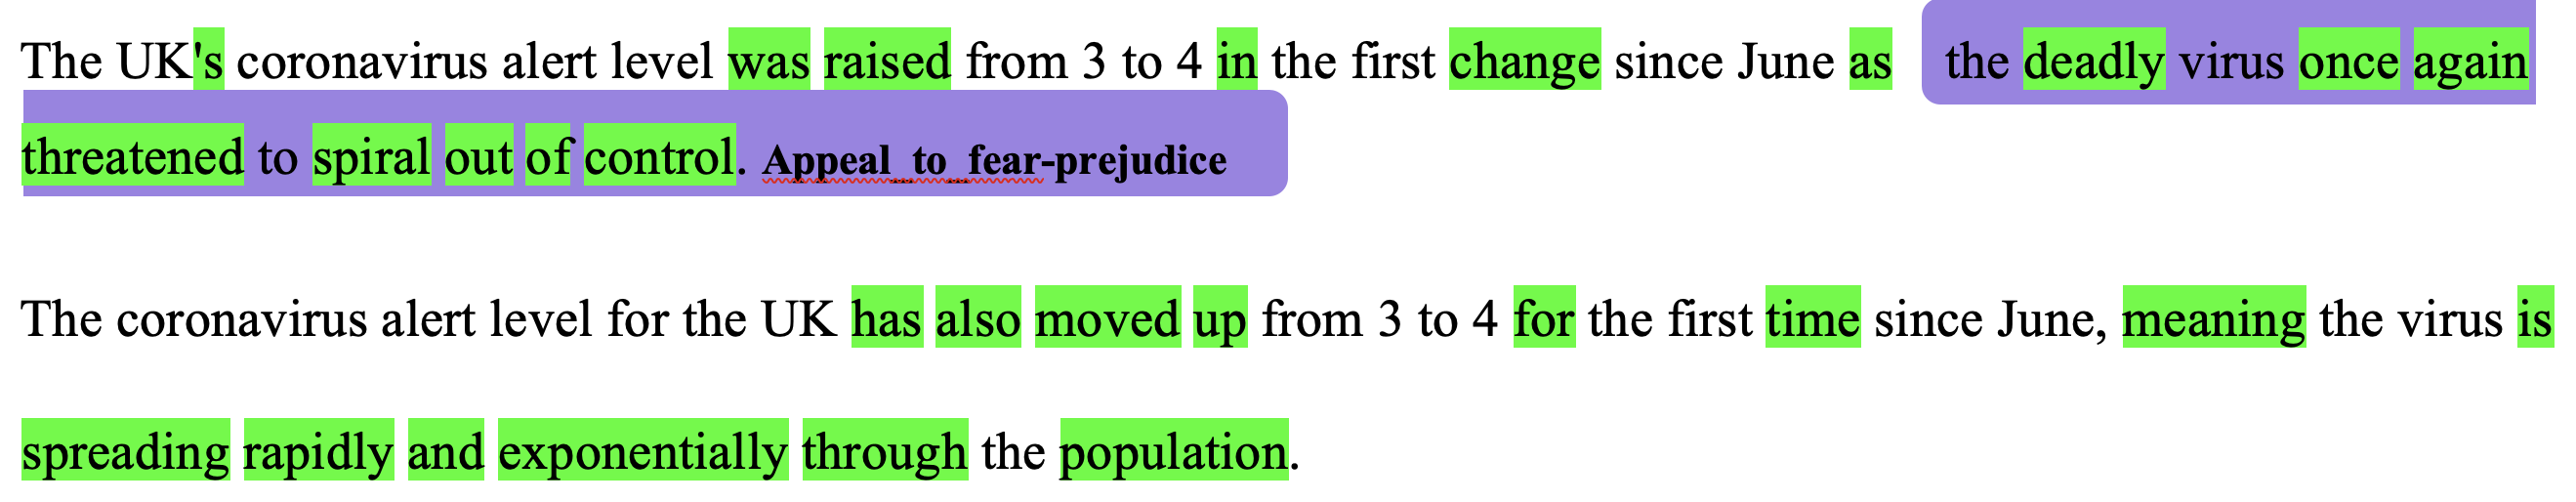
\includegraphics[width=\linewidth]{figures/annotation_212_annotated.png}}
    \caption{Pair of sentences annotated by the uniqueness and persuasion analysis.}
    \label{fig:annotated_clique_data}
\end{figure}
% \todoAW{I've missed something, I think... where do you discuss how the detected technique is classified?}
% the answer is in sec:

Figure~\ref{fig:annotated_clique_data} shows a pair of sentences that contain one persuasion technique.
In green we highlighted the words that are unique for the analysed sentence with respect to the other, using the method from the previous chapter.
In purple instead we can see that a specific propaganda technique (\texttt{Apppeal\_to\_fear-prejudice}) has been detected.
Some words (e.g., ``deadly", ``spiral out of control") are both unique to the first sentence and also belong to the technique of \texttt{Apppeal\_to\_fear-prejudice}. Instead in many other pairs of our dataset, the changes do not manifest in terms of persuasion techniques.
Our goal is to understand this relationship between variations and persuasion.

% split between computational results and human judgement
We conduct the analysis following a purely computational approach, meaning that both the detection of variations and persuasion techniques are automated (not coming from a gold standard).
% \begin{enumerate}
%     \item computational-only: we compute how much the differences in wording affect the scores and words of detected persuasion;
%     %\item soft-validation of computational results: we try to see how good the detected changes in persuasion are when we compare to human-generated labels.
% \end{enumerate}
%
% While the first one is less prone to criticism, being computed, the second one is less valid because only I annotated the sentences
% We compute how much the differences in wording affect the scores and words of detected persuasion
We want to measure on average how many variations in percentage also imply a different measured persuasion (in terms of scores). %Are the variations between the texts making the persuasion scores change? 
Furthermore, we also want to analyse if the words changed are also loaded with techniques of persuasion.
% Instead on the validation side with human annotations, we want to check if the results we are getting are 
% \todo{finish sentence}

There could be also an approach based on additional manual annotations, to check the validity of the results with human-based judgement (e.g. to validate whether the extracted persuasion is perceived as different in sentence pairs or not).
However, in the scope of this thesis, we choose to compute the results using only automated approaches.
\todoHA{this paragraph is odd. It doesn't explain what was your rationale for your choices. Perhaps move it to discussions, or justify your choices more clearly}


% Results
% The results have a first quantitative side and then also a qualitative one. ? rename to automated vs manual???
% it depends on which persuasion technique is considered.

\subsubsection{Results}
\label{ssec:lp_relationship_small_variations_quant}

% \todo{compute metrics from results
% Quantitative results\\
% - reduce groups to pairs: select rows and merge\\
% - count statistics about dataset: number of pairs\\
% - find example and create figure with sentence pairs with scores, words\\
% - add propaganda features (score and words) to each csv and merge sentiment analysis (score and words)\\
% - compute score results: score changes average for each technique (shows which techniques are mostly affected by variations)\\
% - compute words results: \#words persuasion / \#words changed\\
% - plot results (techniques vs percentages)
% }
% quantitative
Firstly, we present here some statistics about the \emph{Small Variations Dataset}.
Across the 138 samples included in the dataset, we have on average $32\%$ of the words that are unique. The words that count as unique in a sentence pair are the ones that only belonging to one of the two sentences of the same pair (uniqueness score defined in~\ref{sec:cgs_clustering_and_differences_uniqueness} $u_w = 1$). This corresponds in our example of Figure~\ref{fig:annotated_clique_data} to the words highlighted in green.

\begin{table}[!htbp]
    \centering
    \begin{tabular}{r|rr}
         Technique & sentence-based \% & word-based \% \\
         \hline
         any & 89.8\% & 14.8\% \\
        sentiment\_total & 89.8\% & 12.5\% \\
        propaganda\_any & 10.1\% & 3.2\% \\
        PROPAGANDA:Loaded\_Language & 4.3\% & 0.8\% \\
        PROPAGANDA:Doubt & 0.7\% & 0.5\% \\
        PROPAGANDA:Flag-Waving & 1.4\% & 0.6\% \\
        PROPAGANDA:Name\_Calling/Labeling & 1.4\% & 0.3\% \\
        PROPAGANDA:Appeal\_to\_fear-prejudice & 1.4\% & 0.3\% \\
        PROPAGANDA:Exaggeration/Minimisation & 1.4\% & 0.6\% \\
        PROPAGANDA:Repetition & 0.7\% & 0.1\% \\
    \end{tabular}
    \caption{Amount of detected persuasion techniques across sentence pairs.}
    \label{tab:detected_persuasion_in_variations}
\end{table}

Considering the persuasion analysis, we first start presenting some high-level statistics of which techniques appear in the dataset.
Table~\ref{tab:detected_persuasion_in_variations} shows the quantities of techniques, considering the sentence-level and the word level. The column \textit{sentence-based \%} represents how many of the sentences have the specific technique detected (it is sufficient that a single word is detected to count the sentence). Instead, the column \textit{word-based \%} represent the word-based percentage of the techniques, counting singularly the words that belong to that technique compared to the total number of words in the dataset.

We can see that in $89\%$
%\todoAW{Don't give accuracy to 1 in 1000 when you've only got 138 cases. 2sf is appropriate here.} 
of the sentences, some techniques are detected.
This is almost always caused by sentiment that gets triggered, while propaganda is detected only in $10\%$ of the sentences.
The average word-based percentage (last column, computed for words singularly) that are detected as related to any persuasion technique is below $15\%$,
%\todoAW{Do you count each of the three words in "out of control"? Does that matter?} 
meaning that even though persuasion appears in approximately 9 out of 10 sentences, usually it appears just in a few words.

Breaking down by type of technique, most of these words are detected as carrying sentiment ($12\%$) while less than $4\%$ relates to propaganda.
We can see that the propaganda percentages are much smaller than the values provided by the sentiment tools.
% \todoAW{Is that because of the content of the documents, or the standard of the technology for recognising them?}
By inspecting the samples, we see that generally sentiment detection finds more terms than the propaganda detection. This means that potentially more words are being recalled, but the precision is much lower because we see lots of false positives, despite the combination approach described in Section~\ref{ssec:lp_techniques_sentiment}.

\begin{figure}[!htbp]
    \centering
    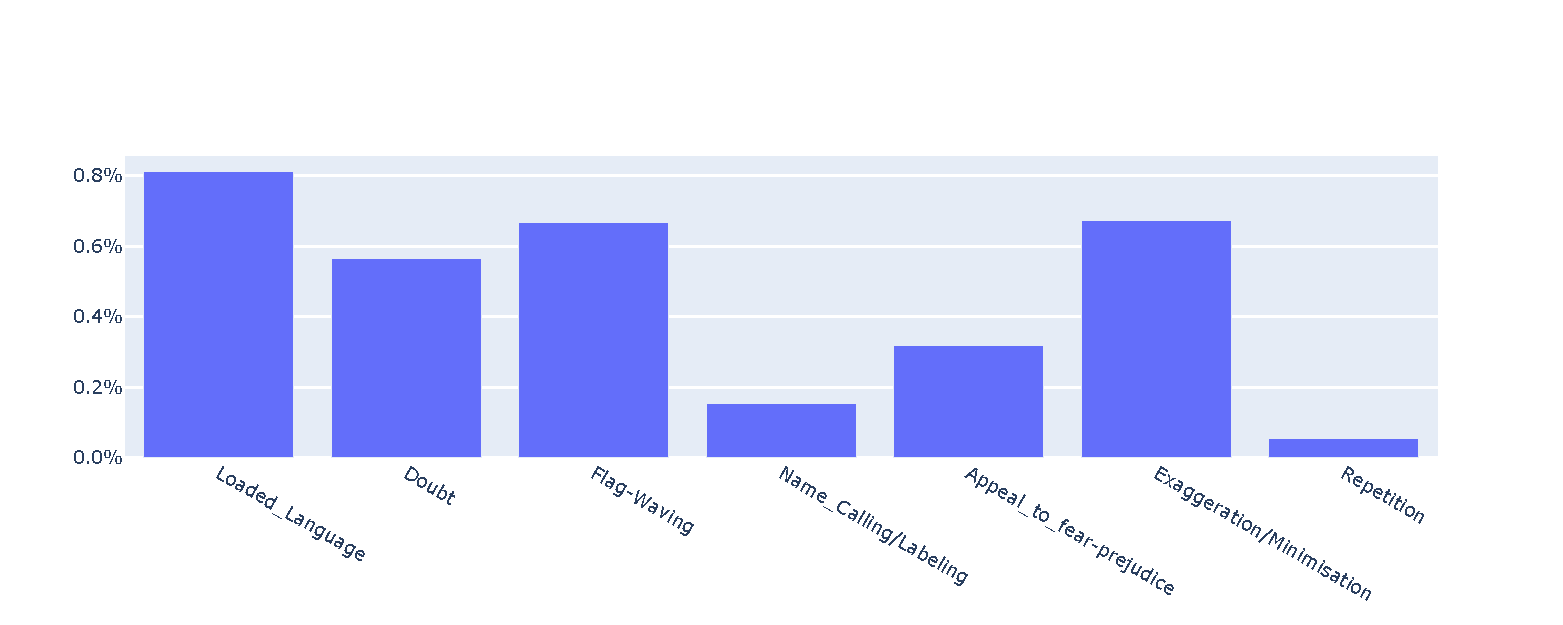
\includegraphics[width=\linewidth]{figures/4.3.1_propaganda_avg.pdf}
    \caption{Average of the detected propaganda techniques across the dataset of sentence pairs.}
    \label{fig:propaganda_avg}
\end{figure}

Figure~\ref{fig:propaganda_avg} shows the percentages of each detected propaganda technique in the corpus (same values as in Table~\ref{tab:detected_persuasion_in_variations}), but filtering by technique only propaganda and considering the last column.
On the horizontal axis, we find the propaganda techniques that appear in this dataset, while the word-based percentage of the corresponding technique is shown on the vertical axis.
The propaganda techniques appearing the most are \texttt{Loaded\_language}, \texttt{Exaggeration/Minimisation}, \texttt{Flag-Waving} and \texttt{Doubt}.

% number of changes vs score variations
The previous statistics were given on the sentences of the datasets without considering their relationship.
In the next paragraphs instead, we analyse the variations together with the techniques.
How many times the variation of the sentences results in a change over the persuasion scores? How big is the change in the scores?
% We answer these question by considering every minimal change in the scores. And then by considering the magnitude of the change.

\begin{table}[!htbp]
    \centering
    \begin{tabular}{r|rr}
         Technique & \% scores changed & avg. magnitude \\
         \hline
         any & 98.5\% & N/A \\
        sentiment\_total & 98.5\% & 9.3\% \\
        propaganda\_any & 14.4\% & 3.4\% \\
        PROPAGANDA:Loaded\_Language & 7.2\% & 1.0\% \\
        PROPAGANDA:Doubt & 1.4\% & 1.1\% \\
        PROPAGANDA:Flag-Waving & 1.4\% & 0.4\% \\
        PROPAGANDA:Name\_Calling/Labeling & 1.4\% & 0.1\% \\
        PROPAGANDA:Appeal\_to\_fear-prejudice & 2.8\% & 0.6\% \\
        PROPAGANDA:Exaggeration/Minimisation & 1.4\% & 0.1\% \\
        PROPAGANDA:Repetition & 1.4\% & 0.1\% \\
    \end{tabular}
    \caption{The impact of sentence-pairs variations on detected persuasion.}
    \label{tab:change_scores_persuasion_in_variations}
\end{table}
% \todoAW{Although this (sentence pairs) is presumably working at the sentence level, which you said you didn't want to do?}
% \todoAW{What's that? (percentage of the allowed interval)}

For each pair of sentences, we compute the persuasion scores by technique, as defined previously in Section~\ref{sec:lp_techniques}:
\begin{itemize}
    \item sentiment score: average of the different sentiment tools, each one normalised to the interval $[-1;1]$;
    \item propaganda techniques quantity: defined as the word-based percentage of the considered techniques.
\end{itemize}
Afterwards, we compare the scores of the sentences belonging to the same pair, and we compute the magnitude of the change (if any).
Table~\ref{tab:change_scores_persuasion_in_variations} shows the results of this comparison.
The column \textit{\% scores changed} is computed by considering whether each sentence pair has different scores (any variation counts). The column \textit{avg. magnitude} instead, expresses the magnitude of the change, measured in percentage of the allowed range for each value ($[min;max]$, namely $[-1;1]$ for sentiment score and $[0;100\%]$).
We can see that in $98.5\%$ of the cases there is a change in the scores of at least one technique.
Breaking down this result, we have that in all these cases (still $98.5\%$) there is a change in the sentiment score. The sentiment detection, not only is picking on more terms (with many possible false negatives), but also is very sensible to the terms used (perturbing the output scores).
Propaganda, on the other side, is detected less and is perturbed less.

\begin{figure}[!htbp]
    \centering
    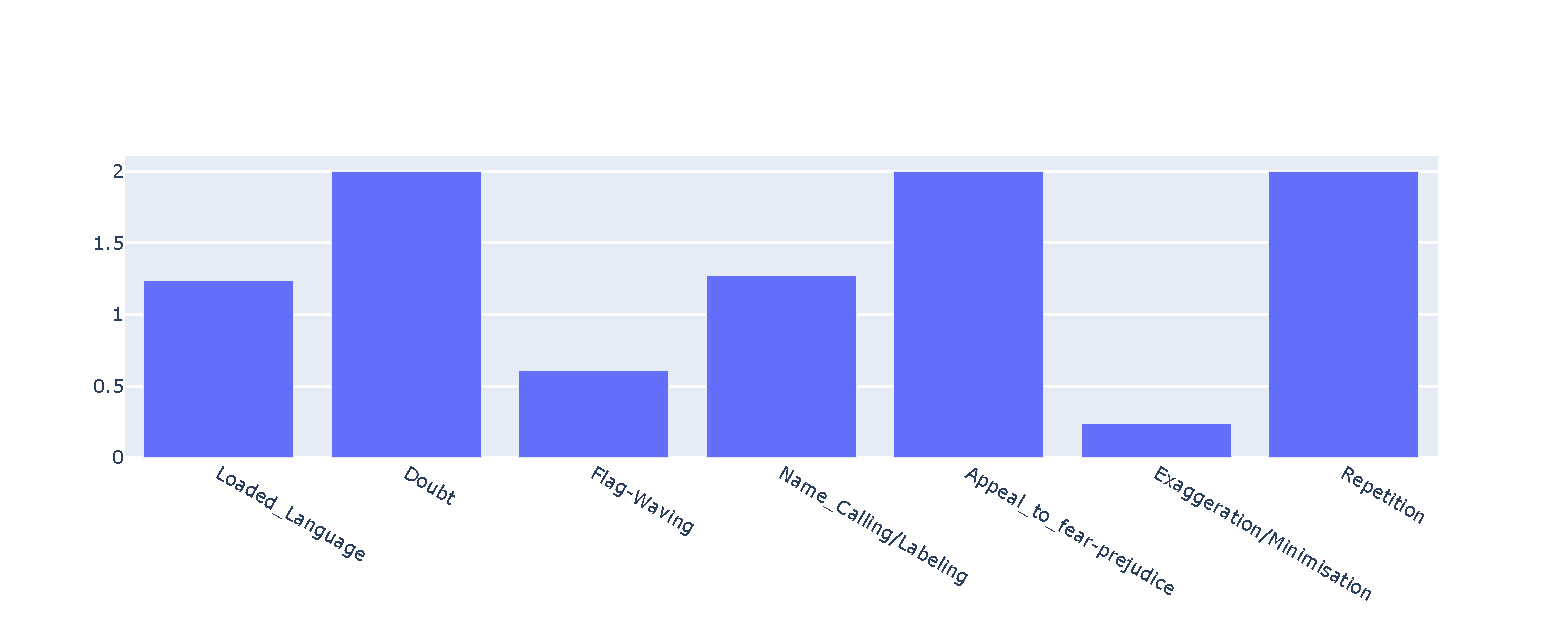
\includegraphics[width=\linewidth]{figures/4.3.1_normalised_ratio_scores.pdf}
    \caption{Normalised ratio between the average variation of the score of each technique, and the average quantity of that technique.}
    \label{fig:normalised_ratio_scores_persuasion}
\end{figure}

We then analyse the ratio between the average magnitude of changes from this table and the average word-based percentages from Table~\ref{tab:detected_persuasion_in_variations} to normalise the results and find the techniques that are mostly affected by this variation.
Figure~\ref{fig:normalised_ratio_scores_persuasion} shows the results of this normalisation.
On the horizontal axis, we have the different techniques that are detected in the corpus, while on the vertical axis the values are computed by dividing the values of Table~\ref{tab:change_scores_persuasion_in_variations} with the values of Table~\ref{tab:detected_persuasion_in_variations}.
%represent how the technique is affected by having the same details provided by two different sentences.
The most affected techniques are \texttt{Doubt}, \texttt{Appeal\_to\_fear-prejudice} and \texttt{Repetition}.
It is important to normalise to discount the effects of the natural disproportion of the techniques used.
For example, loaded language is the propaganda technique most used in general, but as we can see in the figure, it is not the one that changes the most between the pairs of sentences. This could be due to the fact that
%\todoAW{why should that apply more to loaded language than to other techniques?} 
most of the news sources tend to describe with loaded words the same events in their race for attention/clickbaitness~\citep{bazaco2019clickbait,davenport2001attention}.
%\todoAW{OK, good that you've got some citations, but I think I'd include a quote as well to clarify exactly what point these authors are making. }
Therefore, using loaded terms is probably the easiest way to compete and make users read an article. However, techniques that are less evident are the ones in which we can see more differences.


Going back to the sentence pair in the previous Figure~\ref{fig:annotated_clique_data}, only the first one contains \texttt{Appeal\_to\_fear-prejudice} to communicate the detail. This is the type of variation we are interested in.
% Overall, on the quantitative side, we see that a portion (\%?) of the variations in the texts is causing a persuasion score change. Out of X couples of sentences with small variations, only for Y we see a change. Among these, Y1 are changes to the sentiment and Y2 to the propaganda score. The breakdown by techniques is illustrated in the blue bars of Figure~\ref{TODO}, which shows the percentages of variations that correspond to a change in the respective technique. (for each technique, for each sentence pair, a boolean yes/no where yes corresponds to ``changed" and no to ``unchanged", then counting the percentages of yes) 
%
%number of changes vs persuasion-loaded terms: how many terms in percentage?
Therefore, we also compute another measure: how many (percentage) changed words are also persuasion related? Some words can be unique for one sentence but not be related to persuasion, while others can be both unique and loaded of one/more persuasion techniques.

\begin{table}[!htbp]
    \centering
    \begin{tabular}{r|rr}
         Technique & \%pairs & \%words \\
         \hline
         any & 86.9\% & 18.8\% \\
        sentiment\_total & 85.5\% & 17.0\% \\
        propaganda\_any & 10.1\% & 2.9\% \\
        PROPAGANDA:Loaded\_Language & 5.7\% & 1.0\% \\
        PROPAGANDA:Doubt & 1.4\% & 0.4\% \\
        PROPAGANDA:Flag-Waving & 1.4\% & 0.1\% \\
        PROPAGANDA:Name\_Calling/Labeling & 0\% & 0\% \\
        PROPAGANDA:Appeal\_to\_fear-prejudice & 1.4\% & 0.7\% \\
        PROPAGANDA:Exaggeration/Minimisation & 1.4\% & 0.6\% \\
        PROPAGANDA:Repetition & 0\% & 0\% \\
    \end{tabular}
    \caption{Comparison of persuasion words against unique words.}
    \label{tab:words_persuasion_in_variations}
\end{table}

In Table~\ref{tab:words_persuasion_in_variations} we show the values of this measure.
The column \textit{\%pairs} is defined as the ratio between the number of sentences where at least one word of persuasion is also a unique word (not in common with the other sentence in the pair) and the number of sentence pairs. The column \textit{\%words} instead is defined as the total number of words that are both persuasion and unique, divided by the total number of unique words.
In $86.9\%$ of the pairs, we have words that appear only in one of the two sentences that also contain some persuasion. The proportion word-based is $18.8\%$ as we have 2240 words that have been changed (out of 138 sentence pairs, summing the unique words for each pair), and 422 of them are related to persuasion.
We can confirm the results found when using the scores instead of the words. The only differences are in the \texttt{Name\_Calling} and \texttt{Repetition} techniques, that in this case do not overlap with the unique terms.

% All these results are really useful to understand the relationship between the detected persuasion and the variations appearing in multiple versions of the same detail, we have a main limitation which is: does this analysis reflect on what a news consumer would perceive?
% To try to give an answer to this question, we make use of the following subsection which analyses the correlation with human judgements.

% \subsubsection{Computational vs Human Judgement results}
% \label{ssec:lp_relationship_small_variations_qual}

% For this last part of the experiment, we want to understand whether the findings of the previous computational analysis are possibly indicating something that really exists.
% For this reason, we conducted a very limited analysis based on manual annotations.

% TODO

% \todo{
% Qualitative results:\\
% - annotate a subset of pairs: does this change mean something in terms of persuasion? Boolean\\
% - "confusion matrix"\\
% - plot barchart of the ones that behave mostly as predicted\\
% - limitations: because these annotations are done only by me
% }

% Goals:
% - understand how the previous computational results are not just picking any changes. $98.5\%$ of the variation caused a change in the persuasion scores, so we need to assess if we are not only???? 


% Manual annotation of whether the differences in the sentence pairs are making use of different persuasion or relate to a different opinion / point of view. This specific data is used for the experiments ``comparison with manual annotations" at the end of this Section~\ref{ssec:lp_relationship_small_variations_qual}

% % annotations why how and annotation guidelines
% TODO

% Then the qualitative results: do the scores/words represent correctly the persuasion differences? For measuring this, we rely on manual analysis of a subset of sentence pairs. We selected these pairs randomly. We manually label these pairs (How many?)
% (because we don't actually have the ground truth, we are estimating it based on our observations) in two categories: with differences in persuasion or without them.\todoHA{I'm assuming this text not finished?}

% We can define reference values in the following way:

% \begin{itemize}
%     \item \textbf{reference value}: our estimation, but not really a "ground truth";
%     \item \textbf{detected}: whether a persuasion score changes between the two sentences
% \end{itemize}

% Therefore, the true/false positives/negatives for the confusion matrix become:

% \begin{itemize}
%     \item True positive: our estimation is that it should change, and it actually changes.
%     \item False positive: our estimation is that the sentences carry the same type of persuasion, but the detection of persuasion tells that there is something different
%     \item False negative: we deem that the two sentences should contain a change in persuasion, but the detection says nothing
%     \item True negative: no change should be contained, and detection does not detect differences on the persuasion level.
% \end{itemize}

% % results
% The results show???\todo{finish}

\subsubsection{Findings and limitations}

% findings
All the results are really useful to understand the relationship between the detected persuasion and the variations appearing in multiple versions of the same detail.
% quantitative
We have been able to find which techniques change mostly due to the changes represented in our corpus. Furthermore, we understand how a detail may be rephrased to express persuasion.
Being that some techniques appear more (such as sentiment and \texttt{Loaded\_Language}) and some other less, we normalised the variation of the persuasion scores based on the average quantity of each technique.
 By doing that, we discovered that some techniques which are more rare (e.g., \texttt{Doubt}, \texttt{Appeal\_to\_fear-prejudice} and \texttt{Repetition}), are much more probable to occur only in one of the variations of the same detail.
This is particularly meaningful when contextualised to the attention economy~\citep{davenport2001attention}:
%\todoAW{I think you need to flesh this out a bit, although a well selected quote from D\&B should be fine for that.}
the easiest way to capture the attention is to use ``emotional triggers".
Therefore, sentiment and loaded language are the techniques more easy to deploy and we find here that they are more spread to all the versions of the same story.

At the higher level grouping of techniques (sentiment and propaganda, instead of the specific techniques), we found that sentiment detection is providing details that are optimising recall but not precision. We observe that there are many false positives which are disturbing our analysis.
For example, by manually inspecting the samples, we come to the conclusion that not all the changes between the sentences should have resulted in a change of the sentiment score.
This makes it harder to distinguish the cases of word change that really matter. For this reason, sentiment detection might not be the best choice and in the next experiments we decide to use less this feature, in favour of propaganda.

% we have a main limitation which is: does this analysis reflect on what a news consumer would perceive?

% NEED of contextualising the source
One big limitation of our current analysis is that, once we discover how the techniques are related to the variations in the articles, we still do not have a \emph{context} where to place this analysis. We currently lack the information on how to place a news article considering the news source or the author that wrote it.
%\todoHA{unclear. what are you trying to say here?}
For example, propaganda techniques may be used with a political goal or coming from a political standpoint.
We are missing the link between the persuasion used and the original point of view which could motivate such use of techniques.
This limitation will be targeted in the next chapter, considering the perspectives and the political leanings.

% % qualitative
% We then have a set of sentence pairs that only looks like a re-wording with no persuasion changes, and persuasion/propaganda.
% When compared to human juddgement, TODO



% Sentiment

% % sentiment
% Instead for the sentiment analysis, since we want to have detailed information (e.g. which specific words contain sentiment, and with which properties), we are relying on lexicon-based tools. Other more advanced tools (e.g. Stanford CoreNLP) have models which do not provide fine-grained scores but only sentence/document level. (This could be improved)
% % which sentiment lexicons?
% We selected some lexicons: Sentistrength, Vader, and AFINN (TODO description).
% % problems?
% The problem of doing sentiment analysis in this way is that the lexicon is recognised without accounting for other constraints (e.g. POS): we needed to remove some tools because they detected the word "Trump" as being positively loaded (trump as trumpet instead of Donald Trump).


\subsection{\statusgreen Removing Persuasion to Improve Clustering}
\label{ssec:lp_relationship_removing}

The last experiment of this chapter tackles the challenge of analysing the relationship between persuasion and variations in news articles from another perspective.
We approach this analysis from the point of view of clustering.
The previous chapter already analysed the clustering algorithms at the article and sentence level.
Here, instead, we question whether we can help the clustering of articles by removing the persuasion from the articles.

Our \acrshort{rq}2.4 is \emph{To what extent could persuasion techniques be used to identify related news articles?}
%\todoHA{so you are considering that clustering can help recognising events? this is unclear or not well described}}
To answer it, we compare the clustering of the articles when they are complete (not removing anything) against when they have been ``cleaned up" from persuasion.
%\todoHA{Avoid yes/no type of RQs}

% why
The motivation behind this experiment lies in our hypothesis which we described in Chapter~\ref{ssec:lit_layers_of_info}. We hypothesise that news articles are made of two ingredients: topical elements, that are related to events, people, things, and non-topical elements that instead express the opinion of the writer. These two ingredients can be contained in different words or in the same word (cf.~\ref{ssec:lit_layers_of_info}).
In this experiment, by removing the persuasion words, we target both cases but with different effects.
In the case where persuasion words are distinct from topical words, we hypothesise that removing the persuasion words would bring an improvement to the clustering.
Instead, for the case where they appear in the same words, our removal may bring to sentences that are not grammatically complete and may be voided of some topical elements.
%In this experiment, we target only the case where they appear in different words, because it is simpler to separate and see the effect of removal.%\todoAW{But does it invalidate your claims?}
However, we are only considering this simple removal to avoid using more complex models
% For the case where they appear in the same words, we would need to apply some 
(e.g., style-transfer to rewrite the same concepts attenuating/removing persuasion techniques~\citep{bagdasaryan2022spinning}), which is beyond our scope. %\todomargin{ChatGPT citation}
%\todo{if style-transfer is applied, we can also target the cases where they co-live on the same words. check models, there are some for spinning but what about un-spinning?}


% effect of sentiment/propaganda words on sentence clustering
% \todoAW{for doing what? More motivation, this is only operational}

% What: removing the “highlighted” words from the article analysis, the clustering would work better or worse.

% RQ (chap4) 4: Is persuasion an obstacle in recognising the events in multiple articles? (clustering)"

% Why:
% The articles are made of two components:
% the story/event which can be seen from topical words, entities, …
% The layer of framing which here is intended as sentiment-loaded words and propaganda techniques

% Hypothesis
% The framing layer does not help understanding the topics described in the articles. This set of words can be removed to perform clustering better.



% How
To bring this plan into action, we compare the results of  clustering algorithms applied to the full articles against the articles without persuasion terms, to see whether the clustering obtained improves or not.
In the next paragraphs we analyse the dataset used, the approach, the results, and the findings.

% \todo{rephrasing needed for these 3 subsections, at the moment they are quite raw}





\subsubsection{Approach}

Since we want to understand whether by removing persuasion we can have better clustering, our approach is to apply a standard clustering pipeline to two different inputs: first, to the raw articles, and then to the articles with the removed persuasion. So the steps that we do are the following: %\todoAW{This is good... a clear explanation of how you're going to progress.}
\begin{enumerate}
    \item remove persuasion from the article in the first dataset to prepare the second dataset to feed into the pipeline
    \item encode the documents (for both datasets)
    \item run the clustering algorithm (both datasets)
    \item measure the quality of the clusters with the ground truth labels (both datasets)
    \item compare the two cases to determine which one is better
    % \item decide one clustering approach: it needs to be customisable in terms of numbers of clusters
    % \item test the clustering on the articles from the dataset
    % \item measure the accuracy of the clustering with respect to the ground truth
    % \item remove the persuasion terms
    % \item run the clustering on the ``cleaned'' articles, with the same clustering algorithm and parameters
    % \item measure again the predicted clusters with the same metric
    % \item compare the scores and determine which case is better
\end{enumerate}

We carry out this procedure with different number of ground truth clusters, increasing the dataset from an initially small subset.%\todomargin{say this after the description of each step}
The data samples that we use to conduct this experiment is coming from the AllSides dataset presented in Section~\ref{sec:lp_datasets}, as the clusters have a fixed size of 3, which is not as big as the size of clusters of Google News Headlines.

% Test the ability of matching gold clusters with predicted clusters.
% - standard full article
% - removing propaganda/sentiment words

% Seeing if there is an improvement or not when removing propaganda words.

% STEP 1
For the Step 1, we proceed to remove the terms of persuasion with the methods described in Section~\ref{ssec:lp_techniques_sentiment} for sentiment and in Section~\ref{ssec:lp_techniques_propaganda} for propaganda. We input the text articles, and we get in output from the methods the terms that are loaded with sentiment or propaganda techniques. Then we proceed to remove these words from the original articles and we build a second dataset without persuasion terms.
%\todoAWinline{Doesn't this rather assume that the terms can be removed without affecting the meaning? For example, "Johnson heroically took us out of the EU" and "Johnson stupidly took us out of the EU" retain their meaning even if we remove the propagandistic terms "heroically" and "stupidly". OTOH, "Johnson claimed that his actions were legal" and "Johnson proved that his actions were legal" lose their meaning if you remove the loaded terms "claimed" and "proved". Does this matter?}
Additionally, we also have the datasets without only sentiment or propaganda, which come from the original dataset by only removing one of the two persuasion types.
% Removal of the terms: sentiment-loaded terms (multiple lexicons and tools: sentistrength, vader, )
% %And these? AFINN, BING) 
% and propaganda spans (from https://www.tanbih.org/prta).

% STEP 2
For the Step 2, document encoding, we take the approaches 
also used in the previous Chapter~\ref{chap:common_ground_search}: we use for comparison both TF-IDF and \acrshort{use}. The first one is selected to represent simpler approaches while the second one stands for more recent and complex ones. The aim of the comparison is to understand whether there is any advantage of using more sophisticated approaches for this task.
While USE is expected to have better results for complete sentences, we are also conscious that using it with possibly incomplete sentences (removing persuasion terms is not guaranteed to build grammatically complete sentences) could bring to slightly worsened results.
% With both models, output for each document is a numerical representation.
% Document representation:
% Embed the document with the Universal Sentence Encoder / TF-IDF

% STEP 3 
For the 3rd Step, we consider two different approaches: \acrlong{hac} and K-means. The first one (\acrshort{hac}) was used also in the previous chapter, and is very important for us because it does not require to specify the number of clusters wanted. This is ideal for situations where we do not know a-priori the number of topics or headlines that we are looking for. It is also very useful for providing insights at the different levels of the dendrogram (varying the distance threshold), to explore and identify the optimal distances and parameters by observing the intermediate clusters.
Instead, K-means is used to have higher accuracy in identifying the clusters. It works by deciding the number of output clusters in advance.
In a controlled experiment like ours, we know this parameter from the ground truth. %: the number of clusters is the number of different 

% Clustering methods:
% There are multiple clustering methods, and document representations that influence the clustering. We decided to use a method that does not require to specify the number of clusters wanted.
% We started with this specific method (also used in the previous Chapter):
% Hierarchical Agglomerative Clustering (ward method, euclidean distance), which  is very flexible in showing how the clusters evolve when the distance threshold is raised

% STEP 4
For step 4, clustering evaluation, we need to find suitable metrics that can describe how well the produced clusters correspond to the ground truth.
By looking at the literature~\citep{romano2016adjusting,warrens2022understanding}, it emerged that the most used metrics for comparing clusters are \acrfull{ari} and \acrfull{ami}.
The difference between the two is that they are based on different theories. The former is based on pair counting (counting the pairs that appear or not in the same cluster in the reference and in the evaluation), while the latter is based on Shannon Information Theory. In practice, \acrshort{ari} works better when ground truth clustering has large equal sized clusters, while \acrshort{ami} is better when there exist small clusters and ground truth clustering may be unbalanced~\cite{warrens2022understanding}.
% \todoAW{citation?}
Given the statistics of our datasets, we know that \acrshort{ari} will be better to measure the clustering at the \emph{headline} level (reference clusters are always with $size=3$), while \acrshort{ami} will be better for the clustering at the topic level (very different in size, unbalanced).
% \todoAW{I think you need to be more explicit in showing how you come to these conclusions.}



% Clustering evaluation metrics:
% Although clustering is an unsupervised task, we need to see how well the clustering matches with the ground truth annotations of the data. 
% The most used metrics for comparing clustering are:
% Adjusted Rand index,
% Adjusted Mutual Information.



% STEP 5 comparing
For the last step, comparing, we use the two metrics to understand what is the effect of removing the persuasion terms.

% \subsubsection{Results}

% This experiment has several results.

We show the results in the following three paragraphs (1: \acrshort{hac}, 2: K-means, 3: inspection of the predictions), before wrapping up with the findings and limitations. % in Subsection~\ref{ssec:lp_relationship_removing_findings}


% \subsubsection{Data}

% We need some data that contains groups of articles that are related to the same events. There are two different datasets that we can use for having the clustering ground truth:

% TODO: include in approach
% Between these two datasets (AllSides and Google Headlines), we want to be using good quality ground truth for document clustering: so that at least we start from gold-standard groups, defined by human annotators. For this reason, we prefer AllSides with respect to the Google News dataset because it is built and annotated by humans instead of being an output of a clustering algorithm already.

% Step 4 results (curve)
\subsubsection{Hierarchical Agglomerative Clustering}

With \acrshort{hac}, we have the advantage of being able to observe the gradual aggregation into larger clusters.
Therefore, in this paragraphs we observe the effects of increasing the distance threshold in hierarchical clustering.
% , we see how the metrics of \acrshort{ari} and \acrshort{ami} behave.

The value of the metrics can be computed by comparing the ground-truth clustering with the predicted one.
We are using the AllSides dataset, so we just consider the groupings of the headlines (triples) or topic labels (more large clusters) to be the ground truth.
By plotting the metric values against the increasing threshold of distance of the \acrshort{hac}, we can observe how both \acrshort{ari} and \acrshort{ami} increase until a certain point, then decreases again.

\begin{figure}[!htbp]
    \centering
    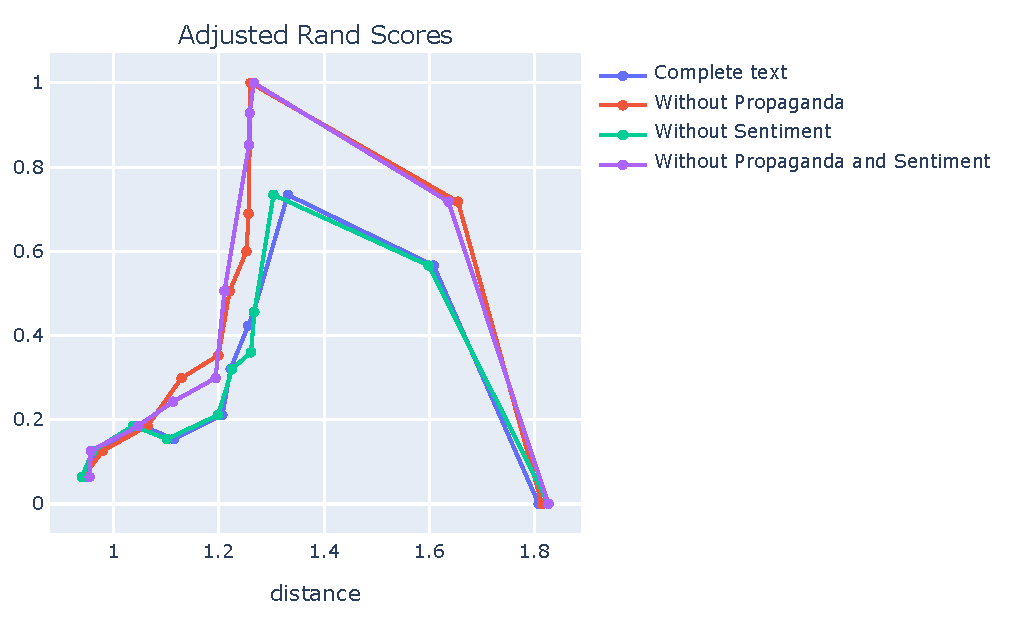
\includegraphics[width=\linewidth]{figures/sentpropnoise_4_en_tfidf_fitness_topic-cropped.pdf}
    \caption{\acrshort{ari} on a simplified scenario (only 4 clusters to identify) using \acrshort{hac} on TF-IDF features.}
    \label{fig:hierarchical_sentpropnoise_evolution}
\end{figure}

Figure~\ref{fig:hierarchical_sentpropnoise_evolution} shows the values of \acrshort{ari} for a simplified case, where only $4$ headlines are considered.
On the $x$ axis, we have the Euclidean distance which corresponds to the current progress of clustering: from the left to the right, initial small clusters are merged and become bigger.
If we observe the line for \textit{complete text}, we can see that it starts on the left with increasing values, then reaches the maximum in the centre and then the score goes down again. At the beginning and at the end, the value is low because the distance threshold is either too tight (left) or too relaxed (right) and the corresponding evaluation clusters are too small (left) or too big (right).
At the center it is more similar to the ground truth, so both the \acrshort{ari} and \acrshort{ami}
%\todoAW{You haven't told me what these are yet, I don't think. Where do you explain how they are calculated?}
scores are higher.

% The interpretation of this curve is that, when the hierarchical clustering begins to raise the threshold, the clusters match more with the gold clusters, until a certain point where distinct clusters are merging together and therefore lowering the scores.
At this point we do the comparison with the other collections of articles where each one of them has been cleaned from sentiment and/or propaganda words. We see in this figure that, while sentiment does not seem to have much impact on clustering, removing propaganda increases the ability to cluster more similarly to the reference. 

% We can compare the behaviour of this curve between the full text and the text without the loaded/propaganda pieces.
The comparison can be performed at the maximum point, where the threshold is optimal, % (we should truncate the clustering there)
or we can compare the full curve. For simplicity, we compare the maximum value of the curve, that in this case is $1.0$.
%reporting also the distance where it has been reached.
Nonetheless, the full curve shows the same results, as seen in the figure above (higher maximum point, higher curve).

As the figure shows, removing propaganda helps TF-IDF reaching 100\% perfect clustering with threshold 1.26 euclidean distance (12 articles on 3 topics: Supreme court, Elections, Coronavirus, Supreme Court). Instead without removal, TF-IDF misplaces some elements.


% table: step 5 results? Check
\subsubsection{K-Means}
For evaluating the effects with different sizes of datasets, we show here some results with K-Means.

% \todoAW{Don't have huge captions like this... move the description of the table into the body of the text.}
\begin{table}[!htbp]
\resizebox{\textwidth}{!}{%
\begin{tabular}{r|r|r|llll|llll}
 &  &  & \multicolumn{4}{c|}{Headlines clustering} & \multicolumn{4}{c}{Topic clustering} \\ \cline{4-11} 
\multirow{-2}{*}{\#headlines} & \multirow{-2}{*}{\# articles} & \multirow{-2}{*}{\# topics} & \multicolumn{1}{l|}{Full text} & \multicolumn{1}{l|}{No sentiment} & \multicolumn{1}{l|}{No propaganda} & \multicolumn{1}{l|}{\begin{tabular}[c]{@{}l@{}}No propaganda\\ and no sentiment\end{tabular}} & \multicolumn{1}{l|}{Full text} & \multicolumn{1}{l|}{No sentiment} & \multicolumn{1}{l|}{No propaganda} & \multicolumn{1}{l}{\begin{tabular}[c]{@{}l@{}}No propaganda\\ and no sentiment\end{tabular}} \\ \hline
2 & 6 & 2 & \multicolumn{1}{l|}{1.0} & \multicolumn{1}{l|}{1.0} & \multicolumn{1}{l|}{1.0} & 1.0 & \multicolumn{1}{l|}{1.0} & \multicolumn{1}{l|}{1.0} & \multicolumn{1}{l|}{1.0} & 1.0 \\ \hline
4 & 12 & 3 & \multicolumn{1}{l|}{\begin{tabular}[c]{@{}l@{}}.390R\\ .553M\end{tabular}} & \multicolumn{1}{l|}{\begin{tabular}[c]{@{}l@{}}.390R\\ .553M\end{tabular}} & \multicolumn{1}{l|}{\begin{tabular}[c]{@{}l@{}}\cellcolor{green}.645R\\ \cellcolor{green}.798M\end{tabular}} & \begin{tabular}[c]{@{}l@{}}\cellcolor{green}.645R\\ \cellcolor{green}.798M\end{tabular} & \multicolumn{1}{l|}{\begin{tabular}[c]{@{}l@{}}.734R\\ .742M\end{tabular}} & \multicolumn{1}{l|}{\begin{tabular}[c]{@{}l@{}}.734R\\ .742M\end{tabular}} & \cellcolor{green}1.0 & \cellcolor{green}1.0 \\ \hline
10 & 30 & 6 & \multicolumn{1}{l|}{\begin{tabular}[c]{@{}l@{}}.616R\\ .765M\end{tabular}} & \multicolumn{1}{l|}{\begin{tabular}[c]{@{}l@{}}.616R\\ .765M\end{tabular}} & \multicolumn{1}{l|}{\begin{tabular}[c]{@{}l@{}}\cellcolor{green}.634R\\ \cellcolor{green}.771M\end{tabular}} & \multicolumn{1}{l|}{\begin{tabular}[c]{@{}l@{}}\cellcolor{green}.634R\\ \cellcolor{green}.771M\end{tabular}} & \multicolumn{1}{l|}{\begin{tabular}[c]{@{}l@{}}.547R\\ .724M\end{tabular}} & \multicolumn{1}{l|}{\begin{tabular}[c]{@{}l@{}}.547R\\ .724M\end{tabular}} & \multicolumn{1}{l|}{\begin{tabular}[c]{@{}l@{}}\cellcolor{green}.558R\\ \cellcolor{green}.730M\end{tabular}} & \multicolumn{1}{l|}{\begin{tabular}[c]{@{}l@{}}\cellcolor{green}.558R\\ \cellcolor{green}.730M\end{tabular}} \\ \hline
100 & 300 & 35 & \multicolumn{1}{l|}{\begin{tabular}[c]{@{}l@{}}.461R\\ .585M\end{tabular}} & \multicolumn{1}{l|}{\begin{tabular}[c]{@{}l@{}}.455R\\ .584M\end{tabular}} & \multicolumn{1}{l|}{\begin{tabular}[c]{@{}l@{}}.461R\\ .581M\end{tabular}} & \begin{tabular}[c]{@{}l@{}} \cellcolor{green}.467R\\ \cellcolor{green}.599M\end{tabular} & \multicolumn{1}{l|}{\begin{tabular}[c]{@{}l@{}}.271R\\ .513M\end{tabular}} & \multicolumn{1}{l|}{\begin{tabular}[c]{@{}l@{}} \cellcolor{red!50}.260R\\ \cellcolor{green}.516M\end{tabular}} & \multicolumn{1}{l|}{\begin{tabular}[c]{@{}l@{}} \cellcolor{green}.274R\\ \cellcolor{green}.514M\end{tabular}} & \begin{tabular}[c]{@{}l@{}} \cellcolor{red!50}.263R\\ \cellcolor{green}.515M\end{tabular}
\end{tabular}%
}
\caption{Results of clustering applied to TF-IDF features with K-means.}
\label{tab:sentpropnoise_tfidf}
\end{table}


% analysis of results
Table~\ref{tab:sentpropnoise_tfidf} is showing how, from a small corpus to bigger corpora, the effect of removing the persuasion words is changing.
Full text is compared against \textit{no sentiment} (sentiment words have been removed), \textit{no propaganda} (propaganda words have been removed) and \textit{no sentiment and propaganda}. For each row, the values represent the \acrshort{ari} (denoted with \textit{R}) and \acrshort{ami} (denoted with \textit{M} for two different granularities: headline and topic clustering. Higher values represent predicted clusters more similar to the reference ones (improvements highlighted in green), while lower values represent more difference (deterioration shown in red). The different rows represent increasing dataset size.
The different rows represent the number of clusters considered from the AllSides dataset.

We notice that in the first row (2 \#headlines), with only two headlines, the metrics suggest that the evaluation clusters are identical to the reference clusters (score of $1.0$ both \acrshort{ari} and \acrshort{ami}).
In the second row (4 \#headlines), we can see that (as previously in Figure~\ref{fig:hierarchical_sentpropnoise_evolution}) with topic clustering we reach $1.0$ with \acrshort{ari} and \acrshort{ami}, because we manage to match perfectly with the ground truth clusters.
This happens with the removal of propaganda, while the removal of sentiment shows no effects.
With the headline clustering instead, we still have some significant improvements (from $.390R$ to $.645R$, but we cannot reach $1.0$.

In the third row (10 headlines), we still see a similar improvement caused by the removal of propaganda. In this case, the improvement is smaller, both for headline and topic clustering.

Finally, in the fourth row with the biggest subset of data made of 100 headlines, we see that the effects of removing sentiment or propaganda decrease for both tasks. For the headlines clustering, only when removing both sentiment and propaganda we see an improvement with the used metrics, and the improvement is quite small (change of around $1.3\%$ \acrshort{ari} and $2.3\%$ \acrshort{ami}). For the topic clustering, the scores change only of some percentage points, and we also see some degradation on the \acrshort{ari} metric.

% USE table 4.2
For comparison, we compute the same metrics with the same clustering method but this time with a more complex model for document embedding (\acrshort{use}). This sequence model has two main differences with respect to count-based models (e.g. TF-IDF): it accounts for the order of the words, because it is a sequence model, and it can make use of synonyms because it is based on the distributional semantics (semantic similarity based on the context)~\citep{firth1957synopsis}. Since this model accounts for the sequence of words, and since we may remove words and break the semantics of the articles when cleaning from sentiment or propaganda, we need to have this comparison.

\begin{table}[!htbp]
\resizebox{\textwidth}{!}{%
\begin{tabular}{r|r|r|llll|llll}
 &  &  & \multicolumn{4}{c|}{Headlines clustering} & \multicolumn{4}{c}{Topic clustering} \\ \cline{4-11} 
\multirow{-2}{*}{\#headlines} & \multirow{-2}{*}{\# articles} & \multirow{-2}{*}{\# topics} & \multicolumn{1}{l|}{Full text} & \multicolumn{1}{l|}{No sentiment} & \multicolumn{1}{l|}{No propaganda} & \multicolumn{1}{l|}{\begin{tabular}[c]{@{}l@{}}No propaganda\\ and no sentiment\end{tabular}} & \multicolumn{1}{l|}{Full text} & \multicolumn{1}{l|}{No sentiment} & \multicolumn{1}{l|}{No propaganda} & \multicolumn{1}{l}{\begin{tabular}[c]{@{}l@{}}No propaganda\\ and no sentiment\end{tabular}} \\ \hline
2 & 6 & 2 & \multicolumn{1}{l|}{1.0} & \multicolumn{1}{l|}{1.0} & \multicolumn{1}{l|}{1.0} & 1.0 & \multicolumn{1}{l|}{1.0} & \multicolumn{1}{l|}{1.0} & \multicolumn{1}{l|}{1.0} & 1.0 \\ \hline
4 & 12 & 3 & \multicolumn{1}{l|}{\begin{tabular}[c]{@{}l@{}}.287R\\ .403M\end{tabular}} & \multicolumn{1}{l|}{\begin{tabular}[c]{@{}l@{}}\cellcolor{green}.543R\\ \cellcolor{green}.641M\end{tabular}} & \multicolumn{1}{l|}{\begin{tabular}[c]{@{}l@{}}.287R\\ .403M\end{tabular}} & \multicolumn{1}{l|}{\begin{tabular}[c]{@{}l@{}}\cellcolor{green}.543R\\ \cellcolor{green}.641M\end{tabular}} & \multicolumn{1}{l|}{\begin{tabular}[c]{@{}l@{}}.566R\\ .513M\end{tabular}} & \multicolumn{1}{l|}{\begin{tabular}[c]{@{}l@{}}\cellcolor{green}.713R\\ \cellcolor{green}.750M\end{tabular}} & \multicolumn{1}{l|}{\begin{tabular}[c]{@{}l@{}}.566R\\ .513M\end{tabular}} & \multicolumn{1}{l|}{\begin{tabular}[c]{@{}l@{}}\cellcolor{green}.713R\\ \cellcolor{green}.750M\end{tabular}} \\ \hline
10 & 30 & 6 & \multicolumn{1}{l|}{\begin{tabular}[c]{@{}l@{}}.313R\\ .416M\end{tabular}} & \multicolumn{1}{l|}{\begin{tabular}[c]{@{}l@{}}\cellcolor{green}.408R\\ \cellcolor{green}.509M\end{tabular}} & \multicolumn{1}{l|}{\begin{tabular}[c]{@{}l@{}}.313R\\ .416M\end{tabular}} & \multicolumn{1}{l|}{\begin{tabular}[c]{@{}l@{}}\cellcolor{green}.343R\\ \cellcolor{green}.434M\end{tabular}} & \multicolumn{1}{l|}{\begin{tabular}[c]{@{}l@{}}.301R\\ .479M\end{tabular}} & \multicolumn{1}{l|}{\begin{tabular}[c]{@{}l@{}}\cellcolor{green}.331R\\ \cellcolor{green}.507M\end{tabular}} & \multicolumn{1}{l|}{\begin{tabular}[c]{@{}l@{}}.301R\\ .479M\end{tabular}} & \multicolumn{1}{l|}{\begin{tabular}[c]{@{}l@{}}\cellcolor{green}.436R\\ \cellcolor{green}.533M\end{tabular}} \\ \hline
100 & 300 & 35 & \multicolumn{1}{l|}{\begin{tabular}[c]{@{}l@{}}.250R\\ .362M\end{tabular}} & \multicolumn{1}{l|}{\begin{tabular}[c]{@{}l@{}}\cellcolor{red!50}.240R\\ \cellcolor{green}.367M\end{tabular}} & \multicolumn{1}{l|}{\begin{tabular}[c]{@{}l@{}}\cellcolor{green}.251R\\ \cellcolor{green}.372M\end{tabular}} & \begin{tabular}[c]{@{}l@{}} \cellcolor{red!50}.234R\\ .362M\end{tabular} & \multicolumn{1}{l|}{\begin{tabular}[c]{@{}l@{}}.185R\\ .420M\end{tabular}} & \multicolumn{1}{l|}{\begin{tabular}[c]{@{}l@{}} \cellcolor{green}.191R\\ \cellcolor{red!50}.408M\end{tabular}} & \multicolumn{1}{l|}{\begin{tabular}[c]{@{}l@{}} \cellcolor{green}.210R\\ \cellcolor{red!50}.418M\end{tabular}} & \begin{tabular}[c]{@{}l@{}} \cellcolor{green}.223R\\ \cellcolor{red!50}.418M\end{tabular}
\end{tabular}%
}
 \caption{Results of the clustering applied to USE features with K-Means.}
 \label{tab:sentpropnoise_use}
\end{table}


Table~\ref{tab:sentpropnoise_use} shows the results when USE is used to compute the document representations.
The difference from Table~\ref{tab:sentpropnoise_tfidf} is that the vector representations are derived from the USE model instead of computing a TF-IDF representation of the texts.
With respect to the TF-IDF results, we can see that when we remove propaganda from the articles, we have less impact. This time, the improvement is due to the removal of the sentiment from the articles.
% when size increases
Also here, as with TF-IDF, the effects of removing persuasion decay when the dataset increases in size.

% USE meaning
The meaning of these results
%\todoAW{If you're interpreting the results, I'd create a conclusions section.}
is that with such a complex model (USE),
propaganda removal does not help to improve the clustering results, even with a small dataset.
%\todoAW{Doesn't help with what? You haven't really shown how your results answer your research questions.}
Propaganda pieces in an article are usually more than isolated words, and are spans with a longer length. Instead, adjectives (one of the common manifestations of sentiment) are frequently isolated words. USE with respect to TF-IDF is more exposed to the sequence of words, and by inspecting the results of removing persuasion from articles we can see that the sentences are incomplete and cannot stand on their own. For this reason, a simpler model like TF-IDF is being helped by the removal of propaganda, while actually for USE the sentences become broken and the clustering struggles more.

% Discrepancy between AMI and ARI
In the two tables, we see that there are some cases where the \acrshort{ari} and \acrshort{ami} metrics provide opposite direction (improvement vs degradation). In those cases, we need to keep into consideration that the two metrics come from two different theories, and also that the values described above are still relatively close to each others.
Having used a quite small number of data samples for this experiment, these two metrics are showing slight differences and not converging.
%\todoAW{I think you need a much more critical comparison of the two methods, to give some indication of exactly why the methods give the different results that they do.}
% Therefore, moving one article from one cluster to another one, may be seen as improvement or not

\subsubsection{Inspection of the predictions}

% Why? What?
In addition to the analysis of the previous paragraphs, we would like to take a closer look into the predictions, to understand better the quantitative results just described.

For simplicity, we consider the case where we have 10 headlines and we use TF-IDF (corresponding to the third row of table~\ref{tab:sentpropnoise_tfidf}). We choose the TF-IDF result because it is easier to analyse the features and see what is happening.
Let’s consider for inspection the articles belonging to two clusters (IDs given by our experimentation): cluster 0\footnote{\url{https://www.allsides.com/story/biden-leads-vote-count-trump-initiates-legal-challenges}} and cluster 7.\footnote{\url{https://www.allsides.com/story/what-watch-2020-presidential-election}}
They each include three articles, and cover the US elections of 2020. The first one was published on 5th November 2020, while the second on 3rd November 2020. So they are quite similar in the entities mentioned, but the most recent one is centred on the legal challenges initiated for the vote counts while the other headline is still pre-vote (3rd of November was the election day). This means that it is challenging for clustering to differentiate between the two ground truth clusters because a lot of terms in common exist.

\begin{table}[!htbp]
    \centering
    \begin{tabular}{c|c|c}
         & Articles from headline 0 & Articles from headline 7 \\
         \hline
        Full article & 0 0 7 & 7 0 7 \\
        Without propaganda & 0 0 7 & 7 7 7
    \end{tabular}
    \caption{Inspection of how clustering changes when removing propaganda.}
    \label{tab:sentpropnoise_inspection}
\end{table}

% In the K-Means TF-IDF they have been labelled as:
% 1, 1, 0 and 0, 1, 0 with the full text, while 1, 1, 2 and 2, 2, 2 when removing the propaganda and sentiment. The first and last article of cluster 7 are able to be grouped to the cluster 7 instead of cluster 0.

% The ground truth for cluster 0 is here https://www.allsides.com/story/trump-mounts-legal-challenges-biden-gains-ground-vote-count and for cluster 7 here https://www.allsides.com/story/what-watch-2020-presidential-election . They are both about US elections (3 November and 5 November)

% what happened
Table~\ref{tab:sentpropnoise_inspection} shows how the articles belonging to two headlines get clustered when considered in full (first row) and when propaganda is removed (second row).
We can see that one article from headline 7 (the middle one) is clustered together with the ones from headline 0 (first row), while when propaganda is removed, it is correctly clustered together with its companions (second row).

% Term importance
Looking at the TF-IDF features for the articles, we see that when we consider the version without propaganda, terms like \emph{win} (win, winner, ..) are removed. These terms are in common between the two clusters and act as noise for the clustering.
In this way, the distinguishing terms of each headline are able to emerge and have more importance:
\emph{Lead} in cluster 0 (5th November), 
\emph{Patience}, \emph{legal}, \emph{wait} in cluster 7 (3 November).

The removal of these terms helps in the fine-grained differentiation of the stories.
% but may not help with coarse topic clustering
However, when there are many different headlines to identify, these removals can also be detrimental.


\subsubsection{Findings and limitations} % and limitations
\label{ssec:lp_relationship_removing_findings}
% meaning of the results

From this whole experiment, we have the overall finding that removing persuasion from news articles helps to recognise clusters, but only in specific conditions:
\begin{enumerate}
    \item The clusters have to be not too many (less than 100).
    % \todoAW{Is that figure of 100 absolute? Looks very close to your figure of 138 articles. How did you arrive at this number?}
    % \todomargin{138 is for the Small Variations Dataset, here experimental setup is article-level and not sentence-level}
    Increasing the number of ground truth clusters reduces the effect of the removal. This happens because the removal of persuasion words causes also a removal of some topical terms. When the number of clusters considered increases, it increases also the possibility to have more similar clusters. As a consequence, the clustering is penalysed because some topical words have been removed, and the \acrshort{ari} and \acrshort{ami} measures decrease.
    \item For count-based models, the improvements are better when propaganda is removed. These terms act as noise and it is better to remove them to allow the topical words to have higher weights.
    \item For language models like USE, removing propaganda can in some cases be detrimental because the sentences lose the semantics on which these models work.
    \item The findings are analogous both for \acrshort{hac} and for K-means.
\end{enumerate}

% Slightly easier to cluster when sentiment and propaganda words are removed from the corpus.
% So propaganda and sentiment are acting like noise in clustering.

There are some limitations to this experiment. Some of them are a direct consequence of the conditions listed above:

\begin{enumerate}
    \item When increasing the size, the difference on the metrics used become smaller and smaller. This means that this approach does not scale well to thousands of headlines. This is, as explained above, a consequence of the topical words being accidentally removed when removing the persuasion words.
    % \todoAW{Is this a consequence of the curse of dimensionality? If so, it's worth being explicit about it. It's worth being explicit if it isn't, come to that...}
    \item Removing terms from articles makes them incorrect grammatically. For TF-IDF encoding, this is not a problem. Instead, for USE it becomes problem, as this language model encodes the sentence based on the sequence of words received. If the sentences do not make sense, their encoding diverges and we cannot use successfully these representations to cluster the articles together.
    %\todoAW{What exactly is the problem, and how does it affect your analysis?}
    \item Since some words belong both to persuasion and to the topic, by removing them it becomes more difficult to form the correct cluster.
    %\todoAW{As my comments have suggested, I think this is a pretty fundamental issue. Even if you don't do any more experiments, I think you probably need a unpick the issues a bit more.}
    This is why using generative models to perform non-persuasive rephrasing~\cite{bagdasaryan2022spinning} could be worth exploring in future works. However, we leave this out of scope as such a model would introduce too many variations difficult to control. %(choice of terms, but still some meaning).
%\todo{There exists some model that rephrase propagandistic content in non-propagandistic style. What about applying them and compare?}
\end{enumerate}

In addition, we could benefit from knowing more information about the sources of the pieces of text included. This information could contextualise the articles and potentially allow us to find groups of sources that are easier to cluster together than others. This will be considered in the next Chapter~\ref{chap:political_sides}.

Or also, it could be useful adding the information about the topic of the article to find if different topics behave in different ways. The topics will be introduced in our last experimental Chapter~\ref{chap:topics}.

\section{\statusgreen Discussion}

This section contains the discussion of all the results of this chapter. We start with the findings from each of the four Research sub-Questions:

% each RQ
\begin{enumerate}[label={\textbf{RQ2.\arabic*:}},leftmargin=2cm]
    \item \emph{To what extent could we automatically detect the persuasion techniques used by writers?} Sentiment is detected through lexicons and sentiment treebanks. Propaganda, instead, is recognised with deep learning models trained on fine-grained datasets, which can also be quite unreliable (low F1 of $22.5\%$). For populism we do not have detection models, but for our initial findings it seems to be weakly correlated with propaganda.
    %\todoAW{This isn't a discussion, it's a summary.}
    Answered in Section~\ref{sec:lp_techniques}. %\todomargin{this is not a finding/discussion}
    \item \emph{Which persuasion techniques are detected more frequently than others?} We observed that the most common techniques relate to loaded language (through propaganda and sentiment detection). However, the most common techniques are not the ones that differ the most. More subtle techniques, like Doubt and Appeal to fear, are the ones that emerge more when doing a comparative analysis between multiple versions of the same article.
    \item \emph{How do similar news articles differ in their use of persuasion techniques?} In some cases the words that change between multiple versions of the same detail, also cause a change in the detected persuasion. We managed to find that techniques like \texttt{Doubt}, \texttt{Appeal\_to\_fear-prejudice} and \texttt{Repetition} are the ones that are mostly affected by the variations in expressing the same detail.
    \texttt{Loaded\_anguage}, on the other side, is more ubiquitous since news sources are competing for the attention of the reader, and emerges less in a comparative analysis.
    However, in many cases, the differences between the articles cannot be described in terms of differences in detected sentiment or propaganda. This could be due to other types of variation: word choices/synonyms that are not the same word and do not apparently bring persuasion differences.
    %\todoAW{Examples?}
    Or also we have false positives in the detection (especially sentiment) that make it more difficult to see the changed persuasion. Answered in Section~\ref{ssec:lp_relationship_small_variations}.
    \item \emph{To what extent could persuasion techniques be used to identify related news articles?} By removing sentiment and/or propaganda, the clustering of related news articles improves slightly. This improvement is small but it is a sign that the non-topical layer is acting as noise/obstacle in recognising the topical layer. This is a weak verification of our hypothesis presented in Chapter~\ref{ssec:lit_layers_of_info} where we assumed that the news articles are a mix between two layers of topical and non-topical words.  We answered this question in Section~\ref{ssec:lp_relationship_removing}.
\end{enumerate}

% Findings:

% \begin{itemize}
%     \item 
% \end{itemize}

Therefore, we give here an answer to our comprehensive \acrshort{rq}2: \emph{To what extent can we automatically detect the persuasion techniques used in news articles?}

This chapter highlighted how, by integrating the automated detection of persuasion in news articles, we have on one side a clearer idea of the relationship between persuasion and the variations that different news sources produce when reporting events.
On the other side, we have also a deeper understanding of the limitations of the current status of this automated detection, and the repercussions it can have when we use these methods in other tasks.
Computational detection of persuasion means is quite a recent research area, and with time and more resources (datasets and models) it could clearly improve.%\todoAW{Big assumption. I'd rephrase.}

% Our findings from this chapter include:
% \begin{enumerate}
%     \item The relationship between the changed terms and propaganda language is not very straightforward: different parts do not always contain loaded language or propaganda. A lot of changes are not meaningful in terms of propaganda: multiple wording can be unrelated to persuasion. % linguistic variance.\todoAW{Not sure what you're getting at here.}
%     \item Some techniques, such as \texttt{Doubt} and \texttt{Appeal\_to\_fear-prejudice}, appear less in general but are the ones that differentiate more one version from the other. \texttt{Loaded\_language}, on the other side, is more ubiquitous since news sources are competing for the attention of the reader, and emerges less in a comparative analysis.
%     \item As we hypothesised, the persuasion in the articles is adding terms and concepts that create variations (fitting different persuasion goals). As a consequence, these selected words make it slightly more difficult to recognise groups of articles related to the same event.
%     Removing propaganda and/or sentiment from articles makes related articles slightly easier to group correctly in the case where the ground truth of the group is known.%\todoAW{Not sure what you mean by this. In most cases of cluster analysis, there's no meaningful concept of a "correct cluster"}
%     %\todoHA{For what? Not discussed earlier}
% \end{enumerate}
% \todo{check if duplicates of replies to RQs}

\section{\statusgreen Next}
% link to next chapter
In this chapter we investigated the persuasion techniques and how they relate to wording changes in similar sentences and articles.
However, we have not studied the relationship between this observed persuasion in the text and the ideals/agenda/perspective of the author/outlet.
It would be really useful to understand the context around the source of an article in order to interpret its persuasion.
For this reason, the next chapter will consider perspectives and political sides.
In this way we will try to understand if the persuasion of each political side is similar or which are the differences.
Can we observe the different goals that generated the articles (the perspective or political side) also on the persuasion itself? We will investigate what is the relationship between political sides and persuasion.
% If a different goal for the persuasion also can be observed on the persuasion itself.

\chapter{\statusgreen Political Leaning}
\label{chap:political_sides}


% % \digraph{abc}{
%   rankdir=LR;
%   a -> b -> c;
% }


% \digraph{structs} {
%     node [shape=record];
%      rankdir=LR
%     struct1 [label="<f0> left|<f1> mid dle|<f2> right"];
%     struct2 [label="<f0> one|<f1> two"];
%     struct3 [label="hello\gvnewline world |{ b |{c|<here> d|e}| f}| g | h"];
%     struct1:f1 -> struct2:f0;
%     struct1:f2 -> struct3:here;
% }

% \resizebox{\textwidth}{!}{
\digraph{chap5} {
    node [shape=record];
    ingredient [label="new ingredient:\gvnewline Political Leaning"];
    rq1 [label="RQ1: How does persuasion vary across the political spectrum?"];
    rq2 [label="RQ2: Can we predict the political leaning of a news article by observing the propaganda it uses?"];
    rq3 [label="RQ3: Propaganda Detection balanced? Or is there some imbalance in the datasets used in the literature?"];
    
    ingredient -> rq1;
    ingredient -> rq2;
    ingredient -> rq3;
}
% }

\section{\statusgreen Introduction}
\label{sec:ps_intro}

% In this chapter we investigated the persuasion techniques. But we have not studied the relationship between this observed persuasion in the text and the ideals/agenda/perspective of the author/outlet. It can be really useful to understand the context around the source of an article in order to interpret its persuasion.
% For this reason, the next chapter will consider perspectives and political sides. In this way we will try to understand if the persuasion of each political side is similar or which are the differences. If a different goal for the persuasion also can be observed on the persuasion itself.

% In this chapter, we introduce a new factor in our analysis.
In the previous Chapter, %covered persuasion and propaganda,
we demonstrated the need to understand the context around the source of an article in order to interpret the persuasion techniques it contains.
%\todoAW{What are an articles' "persuasion means"?}

% For this reason, 
This chapter introduces the factor of \emph{political leaning}.
Our goal is to understand how persuasion (and more specifically propaganda) varies across the political spectrum.
With news sources that belong to different political orientations, how are propaganda techniques
% across the political spectrum
used differently to persuade the readers?
% If political points of view of the sources can be so diverse, what are the techniques that they use differently in news articles to persuade the readers?
Is there a relationship between the political orientation and the persuasion techniques used?
% How does political point of view influence the usage of propaganda?

% Perspectives and Political Sides. What drives  the variations and propaganda? Which political interests? 

Our Research Question for this chapter is:
RQ3: \emph{To what extent could the use of persuasion techniques help identify the political leaning of a news article?} We can divide it into three sub-questions:

\begin{enumerate}[label={\textbf{RQ3.\arabic*:}},leftmargin=2cm]
    \item How does persuasion vary across the political spectrum?
    \item To what extent can we predict the political leaning of a news article by observing the propaganda it uses?
    % \todoHA{Add question: what are you trying to learn? Most datasets out there are imbalanced}
    \item How balanced are the current propaganda detection methods with regard to political leaning?
\end{enumerate}

% For sub-question 3.1 we use the term \emph{persuasion} that, as described in the previous chapters, encompasses propaganda and sentiment.
% After analysing this first sub-question, we decide to discard sentiment analysis from our next experiments. Therefore, sub-questions 3.2 and 3.3 only target propaganda.

% The difference of terminology (persuasion $\rightarrow$ propaganda) between the first subquestion and the second one is due to the exclusion of sentiment when we reply to the first one,\todoHA{unclear what this means} therefore we only indicate propaganda from there onwards.\todoHA{but you are using all three terms below}
% \todoAW{Have you been explicit about defining the difference between your use of terms "persuasion" and "propaganda"? (If so, where?)}

% % contributions of this chapter
% In this chapter, we find that:
% \begin{enumerate}
%     \item Persuasion is used by every political leaning. With sentiment, it is more difficult to find differences as it appears with similar distributions across political leanings.
%     %\todoHA{unclear}
%     Furthermore, in the previous chapter we have seen how the detection of sentiment-carrying terms produces a high number of false positives.
%     With propaganda instead, we see different quantities of techniques used in the articles, and also some term differences between left and right leaning articles.
%     \item By using the propaganda features only, it is quite difficult to automatically recognise the leaning of a news article. However, when combining the propaganda features together with the features from the State of the Art, we can improve slightly the results (small but statistically significant).
%     \item Propaganda datasets are very imbalanced. Most of the annotated sources and articles are coming from the political right. This may cause problems in the detection of left-leaning propaganda, because during the training no instances of leftist propaganda are being used. This may cause inaccuracies in predicting certain techniques and term usages typical of left-leaning propaganda.
%     %\todoAW{Is left/right leaning a "type of propaganda"? Or do you mean that the types of propaganda used by the political left will be under-represented in the dataset?}
%     % With imbalanced models, we still detect left-leaning propaganda, but we have no idea of how accurate the detection is.\todoHA{rewrite}\todoAW{Could a statistician advise?}
% \end{enumerate}

% For this chapter, we follow a structure that is similar to the one of the previous Chapter~\ref{chap:linguistic_persuasion}:
% \begin{itemize}
%     \item first, in Section~\ref{sec:ps_political_sides}, we introduce the new ingredient: political leaning. We describe the datasets in use and the task of political leaning classification;
%     \item then, in Section~\ref{sec:ps_prop_and_leaning}, we combine the analysis of political leaning with the analysis of the previous chapters. More in specific, we analyse the relationship between propaganda and political leaning. This is the core of this experimental chapter.
% \end{itemize}


% THIS IS FROM OLD 5.3, BUT MOVED HERE TO MAKE 5.3.1 --> 5.3, 5.3.2 --> 5.4 and 5.3.3 --> 5.5 (LESS NESTING

% Here in this Chapter, we want to study the relationship between persuasion and political leaning.
% (studied in the previous Chapter~\ref{ssec:lp_techniques_propaganda} and Political Leaning (just seen in the previous Section~\ref{sec:ps_political_sides}).
After introducing the new ingredient of \emph{political leaning} in section~\ref{sec:ps_political_sides} (definition, datasets and methods), we analyse the relationships it has with persuasion.
% This is the core of this chapter as it analyses the relationship between persuasion and leaning.
In the previous Chapter~\ref{chap:linguistic_persuasion} we analysed persuasion on its own, and we urged to understand better the context around news sources.
In this chapter, we are considering the political leaning as a major factor in differentiating between news sources.
For this reason, we are combining the two analyses with the following experiments:

\begin{enumerate}
    \item Analysis of persuasion features across the political spectrum: we want to understand if we can see some difference between the persuasion techniques of Left, Center and Right (Section~\ref{ssec:ps_prop_leaning_across}, targeting \acrshort{rq}3.1).
    % We are able to identify some differences both in the quantity of specific techniques, and in the terms used.
    With sentiment, it is more difficult to find differences as it appears with similar distributions across political leanings.
    %\todoHA{unclear}
    Furthermore, in the previous chapter we have seen how the detection of sentiment-carrying terms produces a high number of false positives.
    With propaganda instead, we see different quantities of techniques used in the articles, and also some term differences between left and right leaning articles.
    Therefore, we decide to discard sentiment analysis from our next experiments
    This is the reason behind using the specific term \emph{propaganda} instead of \emph{persuasion} in the sub-questions 3.1 and 3.2. 
    \item Automated classification of the political leaning using persuasion features. Can machine learning models differentiate between propaganda and sentiment from left and right? (Section~\ref{ssec:ps_prop_leaning_classifier}, targeting \acrshort{rq}3.2) The motivation of this experiment is that we are able to see some differences from the previous experiment, and therefore we want to see if also machine learning classifiers can differentiate and how well. We find that it is possible to classify the leaning of news articles based on their use of propaganda, but that it is quite hard to be better than classifiers based on the full text of the articles.
    However, when combining the propaganda features together with the features from the State of the Art, we can improve slightly the results (small but statistically significant).
    \item Are the current propaganda datasets imbalanced? (Section~\ref{ssec:ps_prop_leaning_imbalanced}, targeting \acrshort{rq}3.3) Given that the results of both previous experiments (manual and automated) are dependent on the quality of the automated propaganda detection, in this last experiment of the chapter we do an analysis of the imbalance of the data that was used to train the propaganda detector.
    We find that in most of the cases, propaganda examples come from Right-leaning sources and the Left and Center are underrepresented.
    % Most of the annotated sources and articles are coming from the political right.
    This may cause problems in the detection of left-leaning propaganda, because during the training no instances of leftist propaganda are being used.
    This may cause inaccuracies in predicting certain techniques and term usages typical of left-leaning propaganda.
\end{enumerate}






\section{\statusgreen Political Leaning Classification}
\label{sec:ps_political_sides}

In this section, we introduce the concept of \emph{Political Leaning} and the task of \emph{Political Leaning Classification}.

We are considering political leaning as the new ingredient of this chapter. After the introduction at the conceptual level in Section~\ref{ssec:ps_leaning_def}, we investigate and describe the available datasets that are used to perform political leaning classification in Section~\ref{ssec:ps_leaning_data} and then we analyse the existing models for the classification and reproduce the baseline in Section~\ref{ssec:ps_leaning_classifier}.


\subsection{\statusgreen Political Leaning Definition}
\label{ssec:ps_leaning_def}

First of all, we are taking again the definition of political leaning given in Chapter~\ref{sec:lit_leaning}: political leaning is a broad concept that generally describes how someone's ideology is positioned between left and right. This is an oversimplification, and you can find more details in the literature analysis.

The practical definition that we take into consideration is a mono-dimensional feature that varies across an axis that has its extremes in Left and Right, defined with a set of perspectives on common polarising topics.\footnote{\url{https://www.allsides.com/media-bias/rate-your-bias}}

% The extremes of this axis are characterised by known positions against a set of issues. For example, the left has generally an expanded view on LGBTQ+ couples, while the right is usually focused on traditional marriage ``as God intended".\footnote{\url{https://www.allsides.com/media-bias/rate-your-bias}}

% Points from Left and Right ideologies (inspired by AllSides and Wikipedia and cite others) 

% Disclaimer US vs the rest?
% This is based on a set of known perspectives that are generally shared between countries, but can vary based on local culture, traditions, history and recent events.
% \todoAWinline{Isn't this dealt with in ch2? In which case, don't need to labour an oversimplification; just give the definition you're using and refer back.}

What we use in this chapter is a three-class categorisation between Left, Center and Right. As we will see in the next subsection, the number of classes changes based on the specific dataset considered (e.g. 5 classes, with intermediate Left-Center and Right-Center), but we keep a simplified division over three classes.

% Several axes when describing news sources: L/R, factuality, 

\subsection{\statusgreen Datasets for Political Leaning Classification}
\label{ssec:ps_leaning_data}

% Having the task of political leaning classification, the practical definition of leaning comes from the datasets that are used.
For our analysis on the leaning, we have selected resources based on the following criteria:

\begin{enumerate}
    \item publicly available, possibly containing the full text of the articles. If the full text is not available, they may refer to a list of news sources (with political leaning) and therefore we can join this information with datasets that contain full text and news source;
    %\todoHA{not very clear}
    \item relatively large: we need a good number of articles (e.g. $\sim$10k) in order to apply machine learning models;
    \item directly indicate the political leaning of the source/articles. This means that we do not conider datasets that only annotate the news source without asssigning a leaning to the source (e.g., All-the-News or Google News Headlines used in the previous chapters).
    %\todoHA{meaning what?}
\end{enumerate}

We found two broad categories of datasets: the first annotating the news sources, and the second providing collections of articles.
%\todoHA{expand and use examples}
For example, we use Media Bias/Fact Check\footnote{\url{https://mediabiasfactcheck.com/}} which provides a very comprehensive list of news sources. This resource does not provide articles by itself, and we use it in conjunction with datasets that contain the text of the articles and the name of the news source, such as NELA-GT-2018.

% source-level vs author-level
This implies that in most cases, the datasets give a source-based political leaning definition. In other words, that all the articles from a certain news source have the same leaning.
This may generally be true, as each news source has its own editorial processes and perspectives. But in some cases, with guest writers and opinion pieces, the political orientation of a news article can differ from the orientation of the news source.

For this reason, one of the datasets that we consider is \texttt{AllSides} which also considers the political leaning based on the author of the news article. They have source-based leaning labels that are used in the wide majority of the cases (as in the source-based datasets), but in some cases they annotate the articles with the author that wrote them.\footnote{\url{https://www.allsides.com/media-bias/ratings}}

% Datasets annotating sources:

% - MBFC
% - AllSides

% Datasets of articles? Is article always considered with the same leaning as source?

We describe in the following subsections the most relevant datasets used for political leaning classification.



\subsubsection{MBFC Dataset}
% stats updated 15/02/2023

The \texttt{MBFC} dataset contains more than 5600 sources, that are mainly classified across two axes: political leaning and level of factual reporting, as shown in Figure~\ref{fig:mbfc_bbc}.

\begin{figure}[!htbp]
    \centering
    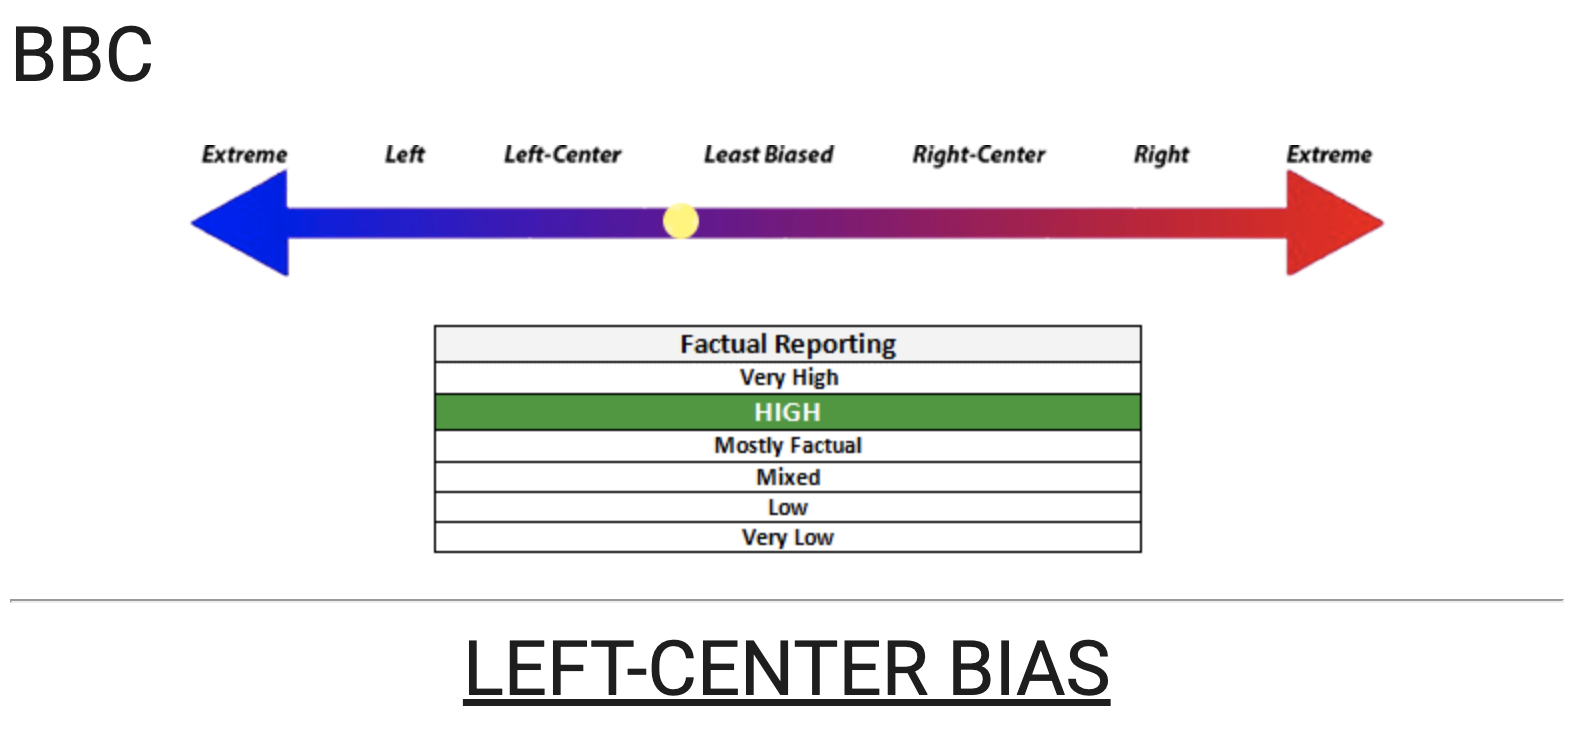
\includegraphics[width=\linewidth]{figures/mbfc_bbc.png}
    \caption{Example of rating from MBFC.}
    \label{fig:mbfc_bbc}
\end{figure}

We are interested in the leaning information, and they are grouped under 5 top-level categories:

\begin{itemize}
    \item \href{https://mediabiasfactcheck.com/left/}{Left Bias}: 351 sources;
    \item \href{https://mediabiasfactcheck.com/leftcenter/}{Left-Center Bias}: 904 sources;
    \item \href{https://mediabiasfactcheck.com/center/}{Least-Biased}: 1202 sources;
    \item \href{https://mediabiasfactcheck.com/right-center/}{Right-Center Bias}: 543 sources;
    \item \href{https://mediabiasfactcheck.com/right/}{Right Bias}: 252 sources.
\end{itemize}

Furthermore, this resource has other special categories, whose sources may also have a political leaning:

\begin{itemize}
    \item \href{https://mediabiasfactcheck.com/fake-news/}{Questionable Sources}: 1483 sources that may contain extreme bias, propaganda, conspiracies, poor sourcing, lack of transparency or fake news;
    \item \href{https://mediabiasfactcheck.com/conspiracy/}{Conspiracy-Pseudoscience}: 438 sources that usually publish unverifiable information lacking evidence;
    \item \href{https://mediabiasfactcheck.com/pro-science/}{Pro-Science}: 214 sources that are based on credible scientific sourcing;
    \item \href{https://mediabiasfactcheck.com/satire/}{Pro-Satire}: 149 sources that are clear that they are satire and do not try to deceive.
\end{itemize}

This dataset does not provide any articles, but it is used as reference by many other datasets in order to estimate the political leaning or the credibility of a news source.

We use this dataset in two different places in this chapter.
The first one, when experimenting with the political leaning classifier based on propaganda features, in Section~\ref{ssec:ps_prop_leaning_classifier}, as its leaning labels are used in the \texttt{NELA-GT18} dataset that we use as a secondary dataset to confirm our findings.
And the second place where we use this dataset is in Section~\ref{ssec:ps_prop_leaning_imbalanced} to analyse the imbalance of the datasets across political leaning and we need its information to place news sources across the political spectrum.

\subsubsection{AllSides Dataset}
% stats updated 15/02/2023

Another very useful resource is AllSides\footnote{\url{https://www.allsides.com/}} which contains two different types of collections:

\begin{itemize}
    \item Sources collection: each source is annotated with its political leaning;
    \item Parallel news collection: \emph{Headline Roundups\texttrademark} made of 3 articles that discuss the same story, one from the Left, one from the Center and one from the Right.
\end{itemize}

\paragraph{Sources Collection}

As mentioned above, AllSides provides leaning annotations that differ from  the ones given only at the source-level.
As can be seen from the Media Bias Ratings published on their website,\footnote{\url{https://www.allsides.com/media-bias/ratings}} they have leaning ratings for different categories: Author (500), News Media (894), Think Tank / Policy Group (108), Reference (25) and Fact-Check (20).

This allows to know the leaning of specific articles written by authors even if they are published on news outlets with a different political leaning. 


\paragraph{Headline Roundups\texttrademark}

The other collection that is very useful from AllSides is the Headline Roundups\texttrademark.\footnote{\url{https://www.allsides.com/headline-roundups}} In this section, the editors regularly publish a hand-curated set of stories. Each of them contains a brief textual introduction of how the story has been framed by the news coverage, and then displays three different articles coming from different political leanings

% is a platform that collects articles from different news sources providing a hand-curated set of stories where articles with opposing political bias are put together, with also a brief textual introduction of the framing differences.

\begin{figure}[!htb]
    \centering
    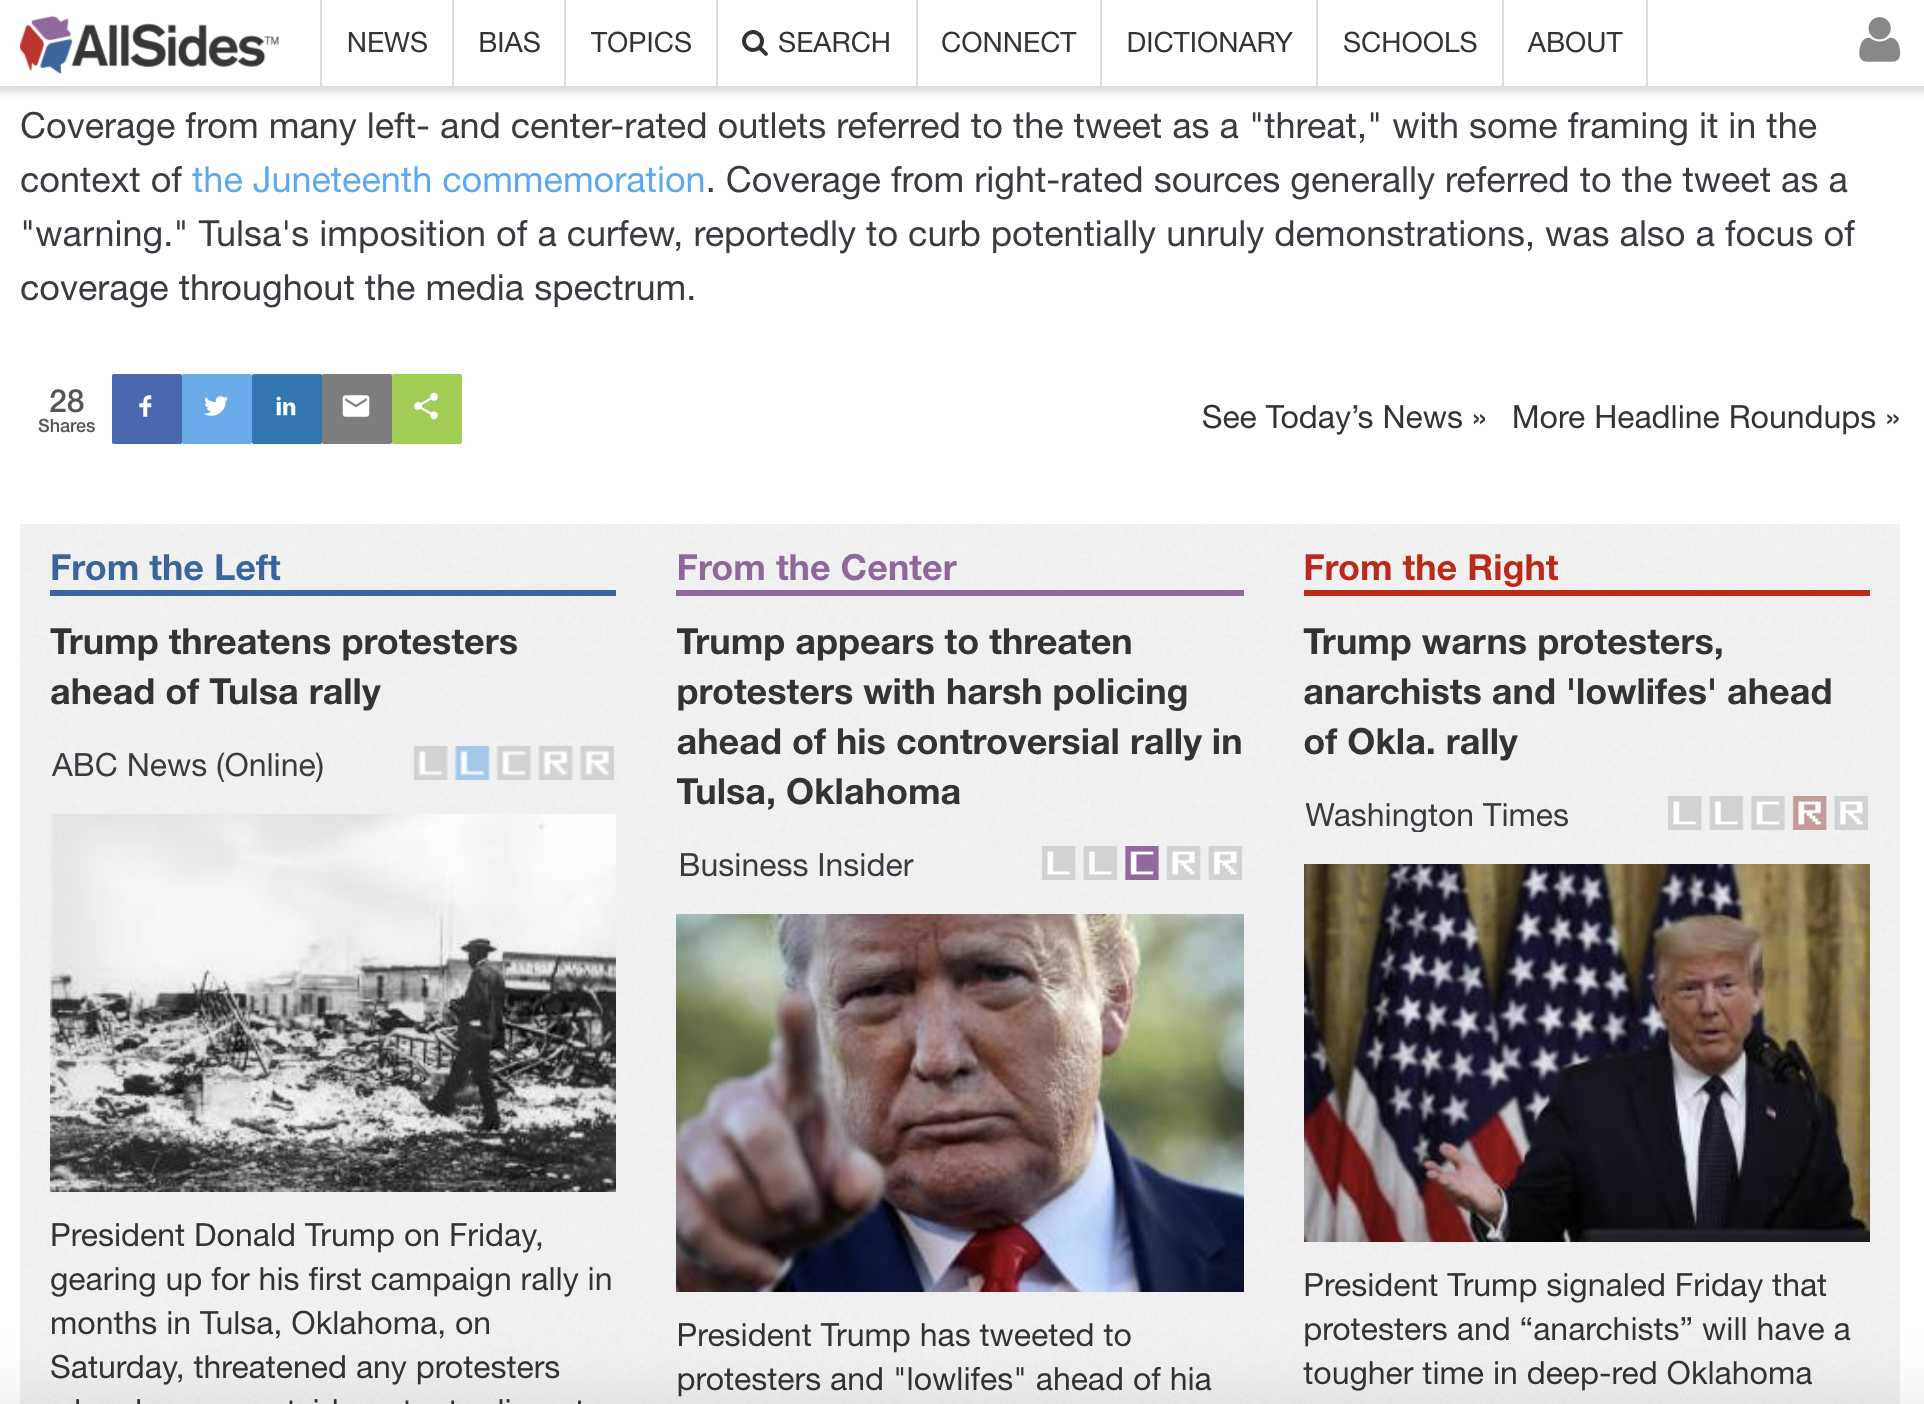
\includegraphics[width=\linewidth]{figures/allsides.png}
    \caption{Example of AllSides Headline Roundup.}
    \label{fig:allsides}
\end{figure}

In Figure~\ref{fig:allsides} we can see an example that displays how a source from the left, one from the centre and one from the right present the story of Trump tweeting about his rally in Tulsa.\footnote{\url{https://www.allsides.com/story/trump-tweets-about-protesters-ahead-saturday-tulsa-rally}}



% - allsides: human-created with interesting framing differences
% Another data source that we actively retrieve is AllSides which provides a curated set of ``headlines''\footnote{\url{https://www.allsides.com/story/admin}} where
The three articles with a different political leaning are put together and compared in their difference.
The curators describe how the story gets framed by the considered sources, using natural language.
This summary usually depicts which terms or themes are used. %\todoHA{sentence unclear}
% At the end of June, we have available 4764 headlines, with 13979 articles linked.
% Differently from Google Headlines which has different versions for each country, 
This data is US-focused being curated in the US and therefore has a limited scope. Also, the discussion of the differences is mainly focused on political issues, without giving much space to other topics.
% role of this specific data
% This data, although the description of the differences is not directly parseable, will be used to feed the user study and understand the role of comparing different sides.


% The work by~\citet{baly2020we} mentions that the annotations are defined on the article level. But in reality, we found that from the dataset all the articles from a specific source have the same leaning annotation. ??? TRUE? OR author level?

% STATS

This collection contains 7,766 headlines (as of 15/02/2023), for a total of 23,298 hyperlinks to articles.
%\todoHA{what's a link here?}
The oldest headlines were published in 2012.

%This is based on the observation 
By analysing the dataset, there are some articles (3.11\%) %(1,080 individual articles, 3.11\% on a total of 34737)
that have a leaning different from their source leaning.
This comes from the fact that some of the articles are annotated with the leaning of the author and not with the leaning of the news outlet, as we discussed before.
% \todoHA{and what does this lead to? which labels do you use?}
This is potentially leading to results that are more specific of the political leanings and less to the news sources. For example, a guest author that presents an opposite point of view with respect to the general alignment of the news outlet would not generate noise for the classifier, but would still produce valid annotated data samples.
Therefore, we use always the most detailed annotations available: political leaning of the author if available, and then as fallback the one of the news outlet.

%To clarify this point, we personally asked to the AllSides team about this discrepancy between article-level bias and source bias, and we understood that there are two types of annotation:
%\begin{itemize}
 %   \item source-level annotation: in most of the cases, the articles are annotated with the bias of the media outlet
 %   \item author-level annotation: sometimes, the articles are annotated with the bias of the specific writer, which can be different from the media bias\footnote{\url{https://www.allsides.com/media-bias/media-bias-ratings\#ratings}}
%\end{itemize}

%Therefore the 3.11\% is due to the author-level annotation. We want to underline that in this way, the annotation of the political leaning is not specifically assigned to the single article but instead it is assigned to the author. It is still a "distant supervision" in some extent.


This dataset has a characteristic that requires an additional data retrieval step in order to be used.
The text of the news articles is not directly provided, but it is made available by hyperlinks that reference the websites of the news outlets.
Therefore, to obtain the text, the hyperlinks need to be followed to scrape the body of the articles (plus cleaning step to remove non-related contents).


% For using this dataset directly, however, there is a limitation. The full text of the articles needs to be separately retrieved by connecting to the corresponding news outlets, and therefore the process of collecting and cleaning the data is not error-free.\todoHA{why introduce this here? how handled errors?}\todomargin{MM: to introduce the next dataset}

% We initially experimented with the data collected from this dataset, but we quickly found the limitation of applying custom data retrieval and also the problem of not having comparable results, as would happen with public and established datasets.\todoHA{rewrite clearly}
% \todoAWinline{I'm confused here. I'm not sure what you've put together yourself, and what you obtained elsewhere. Also, this is rather thin on the actual details of what you did to construct the datasets.}


\subsubsection{Baly dataset}
% \todoAW{Don't have more than three levels}

This dataset is derived from \emph{Allsides Headline Roundup\texttrademark}, as it was built in the work of~\citet{baly2020we} by downloading and cleaning from AllSides and from the respective news outlets all the articles (dataset including headlines until 21 July 2020).

The dataset therefore 
% % FROM TTO2020
% The dataset we use is from~\citet{baly2020we}, and
consists of articles in English language from over 800 sources (majority from the US), labelled for their political leaning (Left, Centre or Right).\footnote{\url{https://github.com/ramybaly/Article-Bias-Prediction}}
This dataset contains several attributes for each article: full text (collected from several news websites and cleaned), political leaning, topic, news source, and author name (attributes from AllSides).
% However, in our models and experiments, we only use the text of the articles to avoid bias associated with the other attributes.
The topic distribution of the articles is uniform across the political leanings, because the dataset comes from triples of articles, one from each political leaning, about the same issue. 
% Authors of this paper publicly provide a dataset, collected from AllSides, where individual articles are labelled for their political leaning.
The dataset contains two pre-splitted folds for training and testing:
\begin{itemize}
    \item \texttt{Random}: where splits are randomly generated. Articles from the same media source may be contained both in the training and testing sets. 
    \item \texttt{Media}; where the articles in the test set are from media sources that do not occur in the training set. %, which is more appropriate for article-based political leaning analysis. 
\end{itemize}

The Media split enables testing classifiers with less potential bias to previously seen sources, which instead happens with the Random split.
Otherwise, what could happen, is that deep-learning models can exploit this data as a shortcut~\citep{geirhos2020shortcut,baly2020we} to simply learn to recognise the style of the news source, and then from it to predict the leaning.
Instead of making the models exploit this information, the \texttt{media} split separates the sources and performs the evaluation on sources that are unseen during the training.
% Although the political-leaning of articles could sometimes be gauged by their sources, there are many examples where articles' political leaning differ from that of their sources, or the sources' leanings are not well known, or the sources themselves are unknown.
% Hence there is a need for such a detection to be independent of where an article came from.      
%and alignment.

\begin{table}[!htbp]
   \centering
   \begin{tabular}{r|c|c|c}
       & train & validation & test \\
       \hline
       Paper media & 22,969 & 5,098 & 1,200 \\
       GitHub media & 26,590 & 2,356 & 1,300 \\
       \hline
       Paper random & 26,828 & 6,709 & 1,200 \\
       GitHub random & 27,978 & 6,996 & 1,300
   \end{tabular}
   \caption{Differences between statistics from in~\citet{baly2020we} and GitHub.}
   \label{tab:baly_size}
\end{table}

Note that there is a discrepancy between the description of the dataset contained in its reference paper and the dataset made publicly available by the authors on GitHub.
The dataset described in ~\citet{baly2020we} contains 34,737 articles, whereas in GitHub\footnote{\url{https://github.com/ramybaly/Article-Bias-Prediction}} it has 37,554 articles (12,590 Left, 10,285 Centre, 13,399 Right). The details of this difference are shown in Table~\ref{tab:baly_size}, and have been reported to the authors.\footnote{\url{https://github.com/ramybaly/Article-Bias-Prediction/issues/4}}

\subsubsection{NELA-GT-2018}

This dataset, published in~\citet{DVN/ULHLCB_2019}, contains $713,534$ news articles coming from $194$ news sources (most frequents, in descending order: The Sun, The Telegraph, The Russophile, Sputnik, New York Post, The Independent, Drudge Report, Evening Standard, The Guardian, BBC, Instapundit, OANN, TruePundit, Daily Mirror, Daily Caller).

For each article, the available attributes are: publishing date, source, title and content.
And then, for each source, there are many attributes that come from MBFC, AllSides, NewsGuard, Pew Research Center, Open Sources, BuzzFeed. Out of these many attributes, the one that refer to the political leaning are: MBFC, AllSides and BuzzFeed. Out of these three classifications, we find that in the majority of the cases, the labels agree and the only cases where they do not agree are between the Center label (by AllSides) and the Center-Left and Center-Right of MBFC. In other words, the systems only differ in the thresholds around the Center.
Instead, the labels from BuzzFeed cover a significantly lower number of sources, and they only have two values (Left and Right), without a Center category.

In Appendix~\ref{app:nela_processing} we present the processing that we have done on this dataset, to create balanced and unbalanced versions of both random and media splits for it.

\subsection{\statusgreen Models for Political Leaning Classification}
\label{ssec:ps_leaning_models}

% How it is computed

% Usual features

% State of the Art

% Problems: learning the source instead of learning L/R task
After having described the datasets, in this section we present the model that we have chosen from the literature (see Chapter~\ref{sec:lit_leaning}) for the task of \emph{political leaning classification}, and then we proceed to reproduce the baseline.

% FROM TTO2020

% Political leaning detection models have been produced for general media sources~\citep{budak} or for 
% specific political corpora such as congressional records~\citep{gentzkow}, political party websites~\citep{yan2017perils}, and political blogs~\citep{ahmed201}.  
% Others focused on inferring the political leaning of Twitter accounts~\citep{Cohen2013ClassifyingPO}, Facebook users~\citep{Bakshy1130}, politicians~\citep{thomas-etal-2006-get}, or political writers~\citep{iyyer-etal-2014-political}. 
% Various analysis methods were used in such studies, such as linguistic analysis \citep{gentzkow}, graph analysis \citep{chen2017opinion}, topic modelling \citep{ahmed201,Cohen2013ClassifyingPO}, support vector machines (SVM) \citep{Bakshy1130,thomas-etal-2006-get}, and neural networks \citep{iyyer-etal-2014-political,baly2020we}.

We focus on detecting political learning of articles in a corpus of general news from a wide variety of sources (from the previous Section~\ref{ssec:ps_leaning_data}). %, using a neural network approach fused with propaganda features. %\todo{description ok?} 

%often used supervised or unsupervised models applied to , or on opinion graph mining~\citep{thomas-etal-2006-get}.

%gentzkow - linguistic analysis 
%yan2017perils - regression models and neural networks
%budak - supervised learning and crowdsourcing
%ahmed - topic models
%Cohen2013ClassifyingPO - SVM and topic models
%bakshy support vector machine 
%thomas - svm
%iyyer - NN
%chen - SVM, LDA

%Most models use supervised or unsupervised machine learning algorithms, trained using source annotations or crowdsourced articles annotations  
 
%underlined that most of the approaches do not generalise well across domains. 
%As~\citet{yan2017perils} underline, three different classifiers trained on different types of texts (domains: congressional records~\citep{gentzkow}, political websites, wiki) result in lack of cross-domain generalisability (classifier trained on different domain struggles to find correct label on another domain, and mixing the training data reduces performance confusing the models).

In~\citet{baly2020we}, authors used a BERT-based model for predicting the political leaning of individual articles. The model takes as input the text of the article and produces one of three labels: Left/Centre/Right. The model is trained with a corpus from AllSides  (the previously described \texttt{Baly} dataset) which groups articles %with their political leaning 
according to the leaning of their source or of their author. %\todo{manually?}
%Authors found that 3.11\% of their 34737 articles from AllSides has a different leaning to that given to their sources (AllSides confirmed that this is due to using author-based leaning). 
%   \item source-level annotation: in most of the cases, the articles are annotated with the bias of the media outlet
 %   \item author-level annotation: sometimes, the articles are annotated with the bias of the specific writer, which can be
 % Similarly to \citet{baly2020we}, in this paper we also focus on classifying articles, regardless of their source and authorship. 


% Problem: learning the source instead of the political leaning
The main focus in~\citet{baly2020we} is to classify individual articles regardless of the source or author. This generalises better with unseen sources, and with cases were there is a difference between the political leaning of a particular article from that of its source.
% Authors found that 3.11\% of their 34737 articles from AllSides has a different leaning to the given to their sources (AllSides confirmed that this is due to using author-based leaning labels for some articles). 
% Other approaches focus on learning the media bias of a the source~\citep{baly2020written,biessmann2016automating}.



\subsubsection{\statusgreen Baseline Reproduction}
\label{ssec:ps_leaning_classifier}
% \todoAW{Very strange place for this section; I'd have expected it in the evaluation part.}
% \todomargin{Section 5.4 is already long enough. I am keeping this here, justifying it}

% Understanding the implicit political leaning of news articles could be seen as an indicative factor for identifying misinformation~\citep{spezzano2021s}. ???

% Our reproduction of classification from text (baselines):
% - TF-IDF
% - BERT


Having described in the previous subsections the relevant datasets and models for political leaning classification, and also being the next sections related to experiments that mix political leaning with persuasion (as described in the Introduction~\ref{sec:ps_intro}),
we present here the reproduction of the baseline of the political leaning classification that is used in the next sections.

Our baseline for article-level political leaning is~\citet{baly2020we}, which is the current state of the art for general purpose political leaning classification.
% Authors of this paper publicly provide a dataset, collected from AllSides, where individual articles are labelled for their political leaning.\footnote{\url{https://github.com/ramybaly/Article-Bias-Prediction}}
Since the source code for this work has not been released, we reproduced the architecture of the model by following the details provided by the authors. %in~\citet{baly2020we}. 
According to the details provided, we embed the articles in the dataset with a pre-trained BERT model (110M parameters, uncased\footnote{\url{https://huggingface.co/google/bert_uncased_L-12_H-768_A-12}}) and use the vectors from the second-to-last layer, as in \citet{baly2020we}. %\todo{unclear} %The model is made of a single dense layer (softmax activation function) which is trained and tested with the splits provided with the dataset in~\citet{baly2020we}.

\begin{table}[!htbp]
    \centering
   \scriptsize
  %\small
    % \resizebox{\textwidth}{!}{
    \begin{tabular}{l|rr|rr}
        & \multicolumn{2}{c}{Random} & \multicolumn{2}{c}{Media} \\
        Model & F1-Macro & Accuracy & F1-Macro & Accuracy \\
        \hline
        \texttt{Majority} & 21.0286 & 46.0769 & 21.0286 & 46.0769 \\
        % \texttt{Baly-API} & 42.3355 & 43.8356 & 42.0523 & 43.6910 & 41.6863 & 41.7993 & & & & \\
        \texttt{Baly-baseline} (0) & 56.4447 & 58.6153 & 40.8647 & 46.2307 \\
        \texttt{Baly-paper} (*) & 80.19 & 79.83 & 35.53 & 36.75 \\
    \end{tabular}
    % }
    \caption{Baselines results compared with~\citet{baly2020we}.}
    \label{tab:results_baselines_classifier}
\end{table}

Table~\ref{tab:results_baselines_classifier} shows the baseline results.
The row indicated with \texttt{Baly-paper} corresponds to the numbers reported in~\citet{baly2020we} (in their table~3, while \texttt{Baly-baseline} represents the results that we got from reproducing the experiments.

The difference is a quite significant drop ($\sim80\% \rightarrow 56\%)$ with the random splits while outperforming ($\sim30\% \rightarrow 40\%$) with the media splits.
\texttt{Majority} baseline, just providing the most common class as output, has quite low results and is considered here just as lower threshold on the other values.


% Note, however, that the results we reproduced differ from those reported in their paper.
This quite big difference could be because of possible slight re-implementation discrepancies, and of the difference between the dataset reported in their paper and the one they shared on GitHub, as discussed previously in Section~\ref{ssec:ps_leaning_data}.%, which is likely to be due to later updates to the dataset. 
% Table~\ref{tab:results_baselines_classifier} shows the results we reproduced, which form our baseline (\texttt{Baly-baseline}). %For reference, we also include the results reported in the baseline model paper (\texttt{Baly-paper}).%, which are significant drop with the random splits while outperforming with the media splits.

Differences in the data and not sharing the implementation make it impossible to reproduce their baseline exactly.
Therefore, \texttt{Baly-baseline} represents our best effort in reproducing it.

In the next experiments, when we refer to the baseline
we mean the reproduction of the baseline as in \texttt{Baly-baseline}. Using the numbers from \texttt{Baly-paper} would not be fair, as the dataset used is different, and we want to exclude any other factors in the comparison of the results.


% TODO table from https://github.com/ramybaly/Article-Bias-Prediction/issues/4


% To test our three Research Questions (Section \ref{sec:intro}), we extend the model above with various propaganda-related features, and compare their outcomes to the baseline to see if and how adding propaganda features affect the classification results.\todo{move to Experiment Setup? and clarify different between when using your model alone vs combining with basline} 


% disclaimer
% Due to the small differences in the dataset and some possible differences also in the implementation of the baseline, we are not able to reproduce the results indicated as ``table 3'' of~\citet{baly2020we}. % We will substitute our implementation with the official baseline if and when its code will be shared. 

% The results of Table~\ref{tab:results_prop_features_classifier} show that the baseline we reproduced (\texttt{Baly-baseline}) achieves different results from the those reported in their paper (\texttt{Baly-paper}): 


%     \item \texttt{Baly-baseline}, being an emulation of what described in~\citet{baly2020we}, is still far from the 80\% results reported by the authors. 


% and we are still waiting for the official code to be released (containing the implementation of their model).


%are comparing this baseline with other similar models where we use features coming from the propaganda analysis (see next) and feeding them to a model with the same single dense layer.

% that we have are going to be tested by comparing the results obtained adding specific features to the reference model. 

% For complete comparability of the results, therefore, we need to use their dataset. However, since the dataset was released only in April 2021, the experiments are also considering our own data collection from AllSides.
% At the moment, we have their dataset available (articles annotated with L/C/R labels) but we still need to finish the automated annotation of propaganda techniques (each article annotated with the 18 techniques), through an API that has quite low rate limits. For this reason we present in the following sections still the results of our own datasets (we have the propaganda annotations of them because the rate limit has been introduced only recently).


% The first dataset, here denoted with \texttt{13k} because of its size, was collected from the Headlines\footnote{\url{https://www.allsides.com/story/admin}} which are groups of three articles, usually one from the left, one from the centre and one from the right (annotated at the author level).
% This results in a dataset made of 13k articles.

% Being this dataset much smaller than the reference one, we performed a second data collection which this time considers also articles that are annotated singularly, not in groups of three as before.\footnote{\url{https://www.allsides.com/unbiased-balanced-news}}.
% This second dataset collected instead has a size of 60k articles.
% The main difference with the first one is that the articles are not grouped in triples of Left/Center/Right. This results in the 60k dataset being much more imbalanced than the 13k (which still is a bit imbalanced because not exactly all the groups keep the balance).

% The third dataset is coming from~\citet{baly2020we} through the official GitHub repository \url{https://github.com/ramybaly/Article-Bias-Prediction}. We observe that there are some differences with what is stated in their paper, as can be seen in table~\ref{tab:baly_size}. What probably happened is that the authors kept collecting more articles.



% Now, by comparing the two different datasets collected with the dataset from~\citet{baly2020we}, Figure~\ref{fig:venn} shows that the 13k and Baly are mostly balanced subsets of the 60k.
% Although the URLs of the articles in the Baly dataset are a subset of the URLs of the articles in our datasets (13k and 60k), the texts of the articles do not match: the data cleaning of \texttt{Baly} is different and better than our data cleaning (e.g. removing non-article content), and having different texts makes the propaganda annotations differ slightly.

% The last dataset considered is derived from the 60k, by keeping it balanced between target labels. Since the smaller group (Center) has 11309 articles, we limited the articles from the Left and Right to contain 11309 articles too, through random selection. We will compare the results of the imbalanced 60k with the balanced 60k.

% TODO: only table or only histogramm
% \begin{figure}[!htb]
%     \centering
%     \includegraphics[width=\columnwidth]{figures/dataset_comparison.pdf}
%     \caption{Distribution of the three datasets across the political spectrum}
%     \label{fig:dataset_comparison}
% \end{figure}

% \begin{table}[!htb]
%     \centering
%     \begin{tabular}{l|r|r|r}
%         Dataset & \#Left & \#Center & \#Right \\
%         \hline
%         13k & 6058 & 2672 & 4408 \\
%         60k & 27457 & 12565 & 20441 \\
%         60k-balanced & 12565 & 12565 & 12565 \\
%     \end{tabular}
%     \caption{Distribution of the three datasets across the political spectrum}
%     \label{tab:dataset_comparison}
% \end{table}

% \begin{figure}[!htb]
%     \centering
%     \includegraphics[width=\columnwidth]{figures/venn.pdf}
%     \caption{Overlap between the three datasets}
%     \label{fig:venn}
% \end{figure}




% - source labels vs author labels?
% \\

% classifier comparison with theirs
% Since at the moment the results are shown from our datasets, the only way to compare with the baseline is to use the same model. For this, we are waiting for their implementation to be shared. In the meanwhile, we have tried to emulate the baseline, based on the description of the model given in~\citet{baly2020we}. We name this set of results with \texttt{Baly-baseline}. However, the results of this model are lower than the official results, so there have to be other differences other than the dataset size increased.
%     \item using a prediction endpoint of political leaning exposed by the same research group. We do not know if this endpoint is an implementation of the model described in~\citet{baly2020we} or not, the results will tell. We name this set of results with \texttt{Baly-API}.
% \end{itemize}
% Instead, for the second big issue of comparability (the model), we need to have their model implementation to compare our results. While the dataset was not shared with us, this was the only possible way to compare: feed our dataset to our models and theirs and compare fairly the scores. We found that their API exposes a political leaning prediction endpoint that accepts sending text and provides the probability of the article to belong to left/center/right. We don't know if this implementation is the one behind the paper (the prediction belongs to the same project at QCRI) but we assume it is.
% Therefore we sent all the articles that we have in our datasets to that endpoint and took the argmax of that prediction. The results collected with this method are annotated here with \texttt{Baly-API}.
% From the description given in their paper~\citep{baly2020we} we tried to reproduce locally the same model. We will observe how much this is the same with the results of \texttt{Baly-API}. These results are annotated with \texttt{Baly-baseline}.
% As soon as the implementation of the model will be shared by the authors, this confusion will be removed.
% \\


% \section{\statusgreen Persuasion and Political Leaning Classification} --> OLD 5.3 intro to 5.3.1, 5.3.2, 5.3.3 is now in 5.1 intro
% \label{sec:ps_prop_and_leaning}


\section{\statusgreen Persuasion Across the Political Spectrum}
\label{ssec:ps_prop_leaning_across}
% From Experiment 4.3: comparison of sentiment/propaganda across political leaning

Our first subquestion for this chapter is RQ3.1: \emph{How does persuasion vary across the political spectrum?}

To answer this question, we perform a comparison across the political leanings to see if we can identify major differences (for example, one leaning could contain more of one specific technique, or differentiate in the terms used).
For this reason, we perform the comparison by considering both the \emph{amount} of each persuasion technique, and the \emph{term frequencies}.

% - overall sentiment and propaganda across spectrum
%     - quantities
%     - terms
% - for each technique, what are the variations
%     - quantities
%     - terms


% Our hypothesis is that more extreme views will contain more persuasion (especially propaganda techniques).\todoAW{Slightly messy use of "hypothesis" here, given the way it's used in statistics. Maybe you want to say that you are investigating whether extreme views contain more persuasion. Then when you set up your experiment, the null hypothesis will be that there's no relationship between persuasion and extremity, and the alternative hypothesis is that extreme views contain more persuasion.}
We are investigating whether extreme views contain more persuasion.
This might be the case because stronger positions are characteristic of the extremes, while moderate and center views may express news in a more neutral way, less filled with persuasion.

\subsection{Experimental Setup}

% in short:
For this experiment, we want to see if there are some differences in the persuasion used by different political leanings, both considering the quantities of techniques and the terms used for the techniques.
% \todoAW{different amounts (which is what the previous para implies), or difference in the type of persuasion used?}
Therefore, we take a dataset, we run it through automated persuasion annotation tools, and then we compare the statistics across political leaning of the articles.

% dataset
The dataset used is \texttt{baly}~\citep{baly2020we}, as described previously in~\ref{ssec:ps_leaning_data}.
We take from it the text of the articles and the label for the leaning, expressed over 3 distinct values: Left Center, Right.
%, Mixed, Not Rated. The first 5 values are properly placed across the spectrum, from left to right. The last values instead are for data that is not clearly aligned with one leaning.
It is important to note that the articles in this dataset are grouped in triples covering the same story, and this grouping makes the topic perfectly balanced across the dataset. For each article belonging to one leaning, there exist two other articles that belong to the other two leanings.
In this way, we do not need to consider the fact that some topics may naturally be more subject to persuasion (e.g. political issues) while other topics may be less (e.g. sports or technology, where the writing style could be less loaded).
Having this link between the articles in the dataset allows us to focus on the comparative results excluding the variable of the topic (for now, but we will introduce the topic as a variable in the next Chapter~\ref{chap:topics}).

% features extraction: sentiment/propaganda
From the text of each of the articles, we then extract the persuasion techniques (sentiment and propaganda, as in the previous Chapter~\ref{sec:lp_techniques}). This gives us for each document a set of words annotated with the corresponding technique. From these annotated words, we compute two features:
\begin{enumerate}
    \item word-based percentage of each technique;
    \item terms for each technique.
\end{enumerate}


% 1. Extraction of propaganda/sentiment
% Each article is analysed independently from the others, using the propaganda detection method and the sentiment lexicons.
% The percentages of words annotated with respect to the total number of words are computed for each article.

% 2. Grouping the percentages by political bias
We then consider the labels given by the dataset (Left, Center, Right), and we aggregate the average of word-based percentages (mean, quartiles, distribution). %This gives an idea of how much of the articles from each political side is detected as sentiment-related or propaganda-related.
We also aggregate the term distributions to compute the term relative importance (TF-IDF) to then understand if the Left, Center and Right are using different words to express their persuasion.

\subsection{Quantities of Persuasion Techniques across Leaning}

Here in this section we show the comparison across leanings of the \emph{quantities} of persuasion techniques.
First we compare the higher-level of propaganda vs sentiment, and then we break down the propaganda techniques, that provide a much more detailed picture. 

\begin{figure}[!htbp]
    \centering
    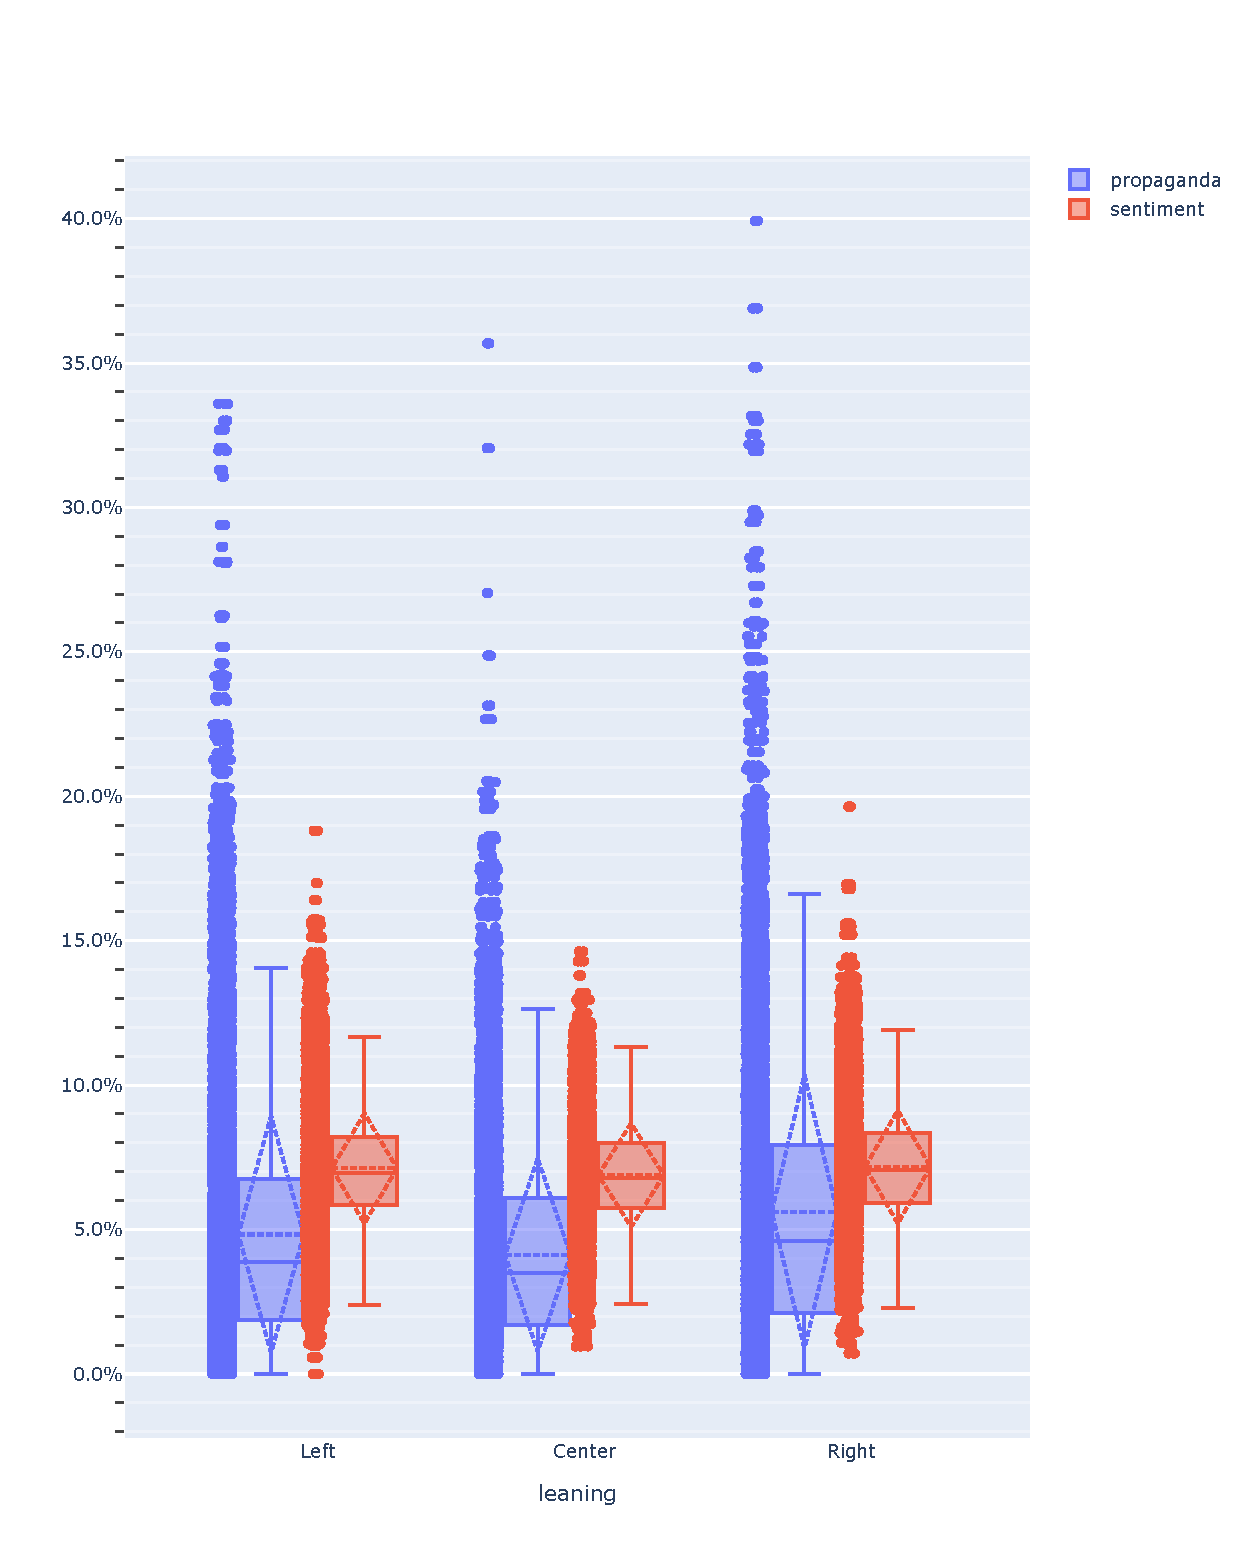
\includegraphics[width=\linewidth]{figures/prop_sent_tech_across_leaning_headlines_mod.pdf} % features_by_bias_box_cleaned_all.pdf
    \caption{Percentage of detected sentiment and propaganda across political leaning.}
    \label{fig:prop_sent_across_leaning}
\end{figure}
% \todoAWinline{Fig~\ref{fig:prop_sent_across_leaning} axis label?}

\subsubsection{Overall Quantity of Propaganda and Sentiment}
Figure~\ref{fig:prop_sent_across_leaning} is a representation which shows the distribution of the ratios computed.
On the vertical axis, the word-based percentage is represented. The boxes represent Q1 (25\% quartile) Q2 (median) and Q3 (75\% quartile). The diamond represents mean and standard deviation, while the whiskers are drawn within the 1.5 IQR value.
% (with data points on the left, and the boxplot with quartiles on the right)
We can see that for sentiment, we have very similar average values and distributions (median, Q1, Q3, mean).
For this reason, we conclude that sentiment is not a good indicator of the differences between political leanings. We cannot find any differences between left and right.

Instead, when we consider propaganda, we see that on the Right we have more words detected as propagandistic.
The Center has slightly fewer words detected in propaganda with respect to the other two leanings (mean values: Center=$4.1\%$, Left=$4.9\%$, Right=$5.6\%$).
This confirms our initial supposition that the center contains less propaganda than more polarised political leanings.

% We did a c

% From this plot we see that there are some very strange values (76\% of highlighted words in one article from the center). Looking at the details, this is an article from BBC which does not look so subjective. The problem is that from the full article, the scraping library only captured the sentence The statement says: ``It is an assault on UK sovereignty and any such use by a State party is a clear violation of the Chemical Weapons Convention and a breach of international law. It threatens the security of us all." which is annotated as almost everything propaganda. For other BBC articles, scraping manages to retrieve the full text without problems.

% There are also a lot of articles which have a percentage of 0\%. Looking at the distribution of the length of the documents, some documents, especially from some sources, have length=0 or a very short length (scraping the cookie disclaimer instead of the full article).
% For this reason a minimum length threshold has been set to cut out these problems: 150 tokens at least.

% This is the same plot, but with the filter on the minimum length.
% We can see that:
% The most annotated side is the Right
% The least annotated side is the Left
% Article from the Center do not contain less sentiment/propaganda (against assumption)
% There are fewer propaganda words than sentiment words

\subsubsection{Quantity of each Propaganda Technique}
% BREAKDOWN BY TECHNIQUE
We then analyse more in detail the breakdown by specific propaganda technique. For this, we keep separated the word-based percentages for each technique.
Our aim is to see whether some techniques are used more in one specific leaning than in the others.


\begin{figure}[!htbp]
    \centering
    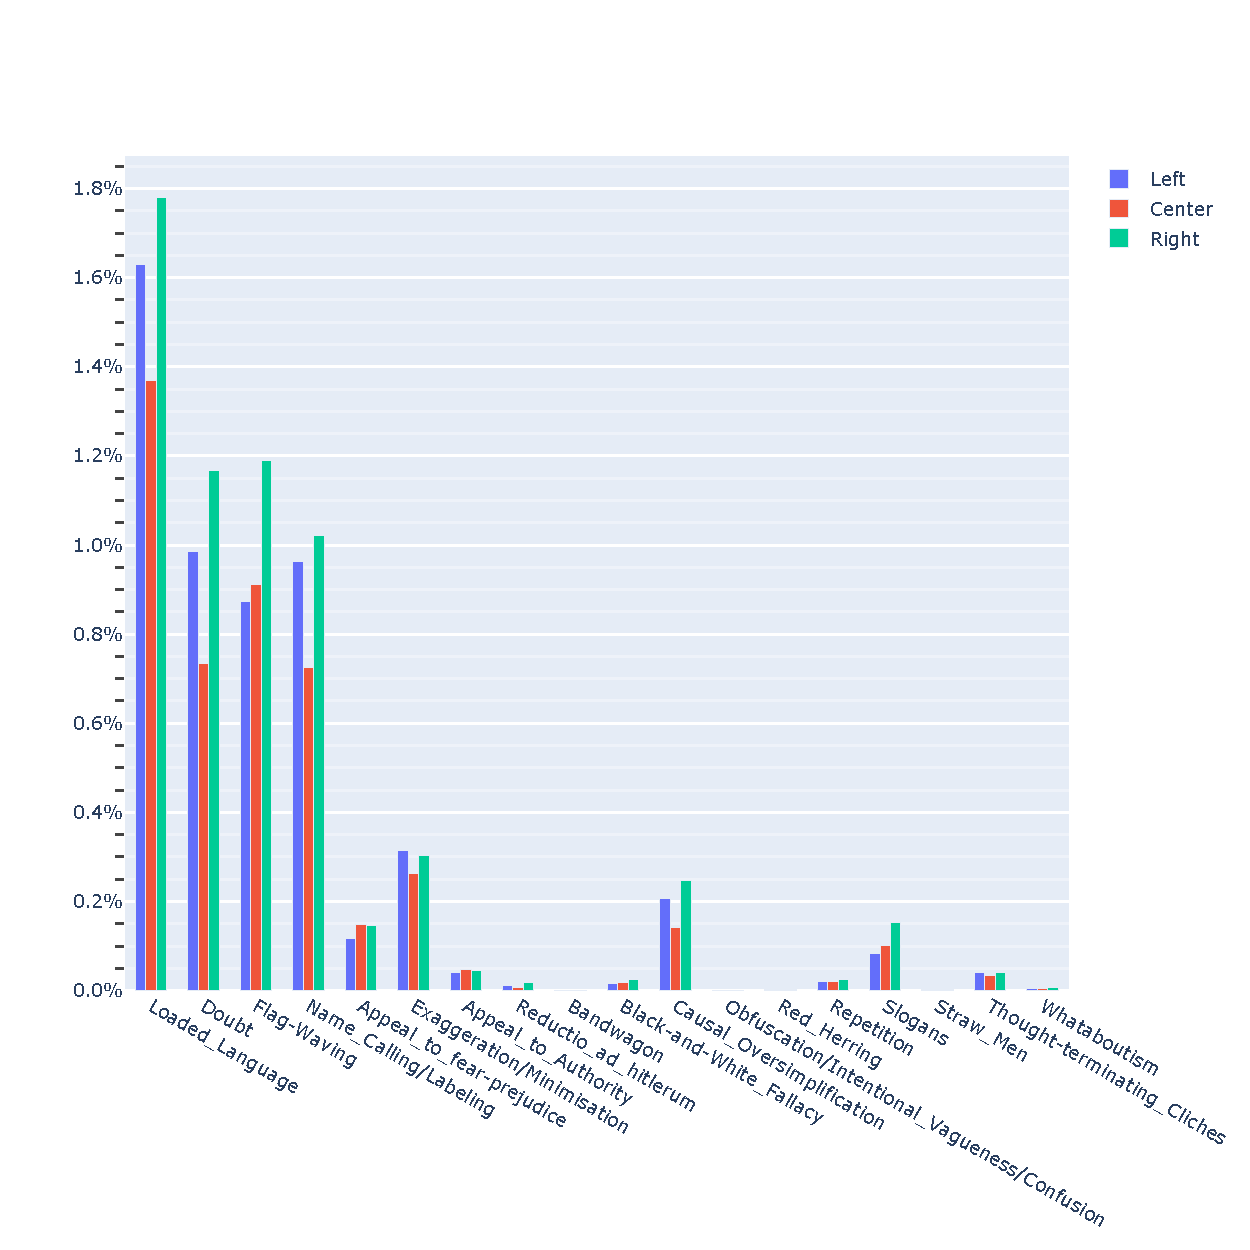
\includegraphics[trim={0 0 0 2cm},clip,width=\linewidth]{figures/prop_tech_detail_across_leaning_baly.pdf}
    \caption{Breakdown of propaganda techniques by political leaning.}
    \label{fig:prop_tech_details_across_leaning}
\end{figure}
% \todo{Fig~\ref{fig:prop_tech_details_across_leaning} Would it be better to show also std deviation or other distribution info like in the previous plot? Or too cluttered?}

Figure~\ref{fig:prop_tech_details_across_leaning} shows on the vertical axis the different propaganda techniques, and each colour represents a different political leaning. The vertical axis represents the mean word-based percentage of the specific propaganda technique for the considered leaning.
With this plot we can compare the techniques across the leanings.

First of all, we notice that the most common propaganda techniques are \texttt{Loaded\_Language}, \texttt{Doubt}, \texttt{Flag-Waving} and \texttt{Name\_Calling/Labeling}.
The articles in the dataset contain on average $1.5$ loaded terms every $100$ words.

% shape analysis
We can see different types of patterns in this plot, which are shown with different shapes over the leanings.
% U-shape
The first one, that we call \emph{U-shape}, happens when the bars of the Left and Right are higher than the bar of the Center. This means that what is represented is polarised on the extremes of the political spectrum.
A good example of this type is the \texttt{Loaded\_Language}, where the Center is using this technique on $1.38\%$ of the words, while Left and Right are using it considerably more.
The same happens with \texttt{Doubt}, \texttt{Name\_Calling/Labeling}, \texttt{Exaggeration/Minimisation}, \texttt{Causal\_Oversimplification}.
These techniques are used by more extreme articles and are giving the general trend that we observed in the previous Figure~\ref{fig:prop_sent_across_leaning}: the center is more moderate and uses propaganda less.

% triangular shape
A second pattern that we notice, is the \emph{triangular shape}. In this shape, the quantities of the technique considered increase (\emph{triangular Right}) or decrease (\emph{triangular Left}) monotonically when going from Left to Right leaning.
This behaviour means that the technique analysed is inherent of a specific extreme of the political leaning spectrum, and constantly decreases when moving to the other side.
It is not surprising that \texttt{Flag-Waving} presents this behaviour, where it is way more detected in Right-leaning articles with respect to Center and even more with Left. This technique is conceptually linked with the principles of nationality, and the strong nationalism is usually associated with Right-leaning political stance.
The same pattern occurs with \texttt{Slogans}. We can link this with the abundance of left-leaning slogans in the recent date range of the dataset for the Trump re-election campaign~\citep{jiang2020political}.

% Reversed U
Another pattern that we see, is the opposite of the first one: \emph{reversed-U shape}. This is characterised by a higher use in the Center than in the extremes.
We can see this pattern with the techniques \texttt{Appeal\_to\_fear-prejudice} and \texttt{Appeal\_to\_authority}. While for the first one, it is imbalanced (highest value center, then Right and then quite less Left), in the second case this is more balanced (Left and Right have similar values).
These techniques may be used with different intents: both for agitate the crowds with strong sentiment (fear and prejudice) or oppositely to moderate and provide as evidences the opinions of the experts (appeal to authority)~\citep{walton2010appeal}. It may be the case that, especially \texttt{Appeal\_to\_authority}, results to be appearing more in the center because of this reason.

\subsection{Propaganda Terms across Leaning}
We then move to the term analysis, to see if we can find any differences in the specific terms used by each leaning.

% One of the first thoughts when comparing terms from different groups, is WordClouds.
% They are a simple and qualitative way to compare distributions of terms.
% Therefore, we computed the WordClouds for the three leanings (Left, Center and Right).


% \begin{figure*}[!htb]
%      \centering
%      \begin{subfigure}[b]{0.3\textwidth}
%          \centering
%          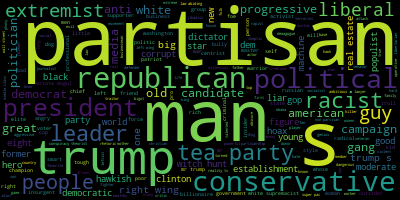
\includegraphics[width=\textwidth]{figures/baly_wordclouds_Name_Calling,Labeling_Left.png}
%          \caption{Left}
%          \label{fig:wc_loaded_left}
%      \end{subfigure}
%      \hfill
%      \begin{subfigure}[b]{0.3\textwidth}
%          \centering
%          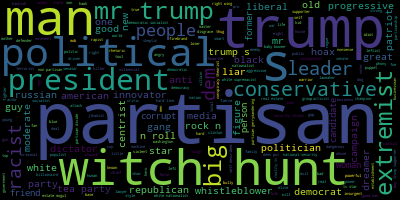
\includegraphics[width=\textwidth]{figures/baly_wordclouds_Name_Calling,Labeling_Center.png}
%          \caption{Center}
%          \label{fig:wc_loaded_center}
%      \end{subfigure}
%      \hfill
%      \begin{subfigure}[b]{0.3\textwidth}
%          \centering
%          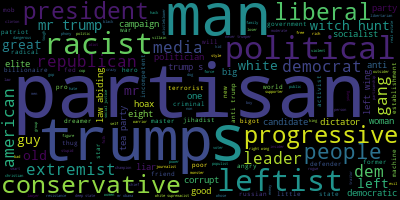
\includegraphics[width=\textwidth]{figures/baly_wordclouds_Name_Calling,Labeling_Right.png}
%          \caption{Right}
%          \label{fig:wc_loaded_right}
%      \end{subfigure}
%         \caption{WordClouds from words belonging to the \texttt{Name\_Calling} propaganda technique}
%         \label{fig:wc_name_calling}
% \end{figure*}

% % Qualitative term analysis done on the words belonging to the different political leanings in our dataset. 
% \todoHAinline{You can't conduce anything from wordclouds. Think of better analysis techniques.}
% \todo{It was an example to then motivate the choice of TF-IDF analysis}
% As Figure~\ref{fig:wc_name_calling} shows, 
By doing a simple ranking of the most important terms for each leaning, we can see some differences in some of the propaganda techniques. For example, considering the \texttt{Name\_Calling} technique:
media sources from the Left appear to frequently use ``republican'' and ``conservative'', while in the Right we can see some unique terms such as ``leftist'' and ``progressive''. Some words are equally used, possibly for different meanings, such as ``partisan''.  
Although these differences, the most repeated word from all the leanings is the word ``partisan'' which is used as a wildcard and probably is intended with different meanings.
But the effect is that most of the terms are repeated in all the leanings, and therefore we have to rely on a better concept than simply counting the term occurrences.

% WHY JUST TERM COUNTING IS NOT ENOUGH: example from wordclouds. Similar terms, just a few are unique of the leaning. The importance of comparing distributions and IDF
This is why we use the concept of relative term importance, %from TF-IDF
% We rely on the concept of term importance, 
as defined by the TF-IDF model: the importance of a term is directly proportional to how many times it appears in the considered document (Term Frequency) and inversely proportional to the number of times it appears in the whole corpus (Inverse Document Frequency).

Here, since we want to understand the relative importance of terms between political leanings, we consider as documents the concatenation of all the selected terms (from propaganda analysis) from all the articles coming from a certain leaning. In other words, we have a corpus made of 3 documents (one for Left, one for Center, one for Right).

We perform this analysis first with all the propaganda techniques together, and secondly by considering each technique separately.

\subsubsection{Propaganda Terms Analysis}
% TERM ANALYSIS OVERALL
For the term importance across all the propaganda techniques, we process each article and select the detected words of propaganda that belong to any of the 18 techniques. Then we collect all these words in 3 buckets, one for each leaning.
We apply on these 3 groups the standard TF-IDF as provided by the \texttt{gensim} library. %(applied on lemmatised words).
This produces a matrix of weights with a shape of $[n_{features}, 3]$ (feature size x number of classes), together with the features names.
Afterwards, we 
computed for each term the difference of the TF-IDF scores between Right and Left.
These values then are used in absolute value to rank the features (words) that differ the most.
This ranking index formulation is therefore:

% absolute value of the difference between the TF-IDF scores of the terms between left and right
$$ i_w = | T_{w,R} - T_{w,L} | $$
where $T_{w,R}$ and $T_{w,L}$ are the TF-IDF scores of the word $w$ respectively in the Right and Left.
Therefore, to identify the features that differ the most between the leanings, we just consider the index just described and we rank the features names accordingly.
% ranked the features based on decreasing this value, as a sorting index computed for each feature.
In this way, we get as first ones the features whose values have the maximal difference.
% These features have high value for the leaning they are mostly occurring in, and lower values for the leaning where they do not appear very frequently.
We can then say that these terms are the most distinguishable propaganda terms across the political spectrum.

\begin{figure}[!htbp]
    \centering
    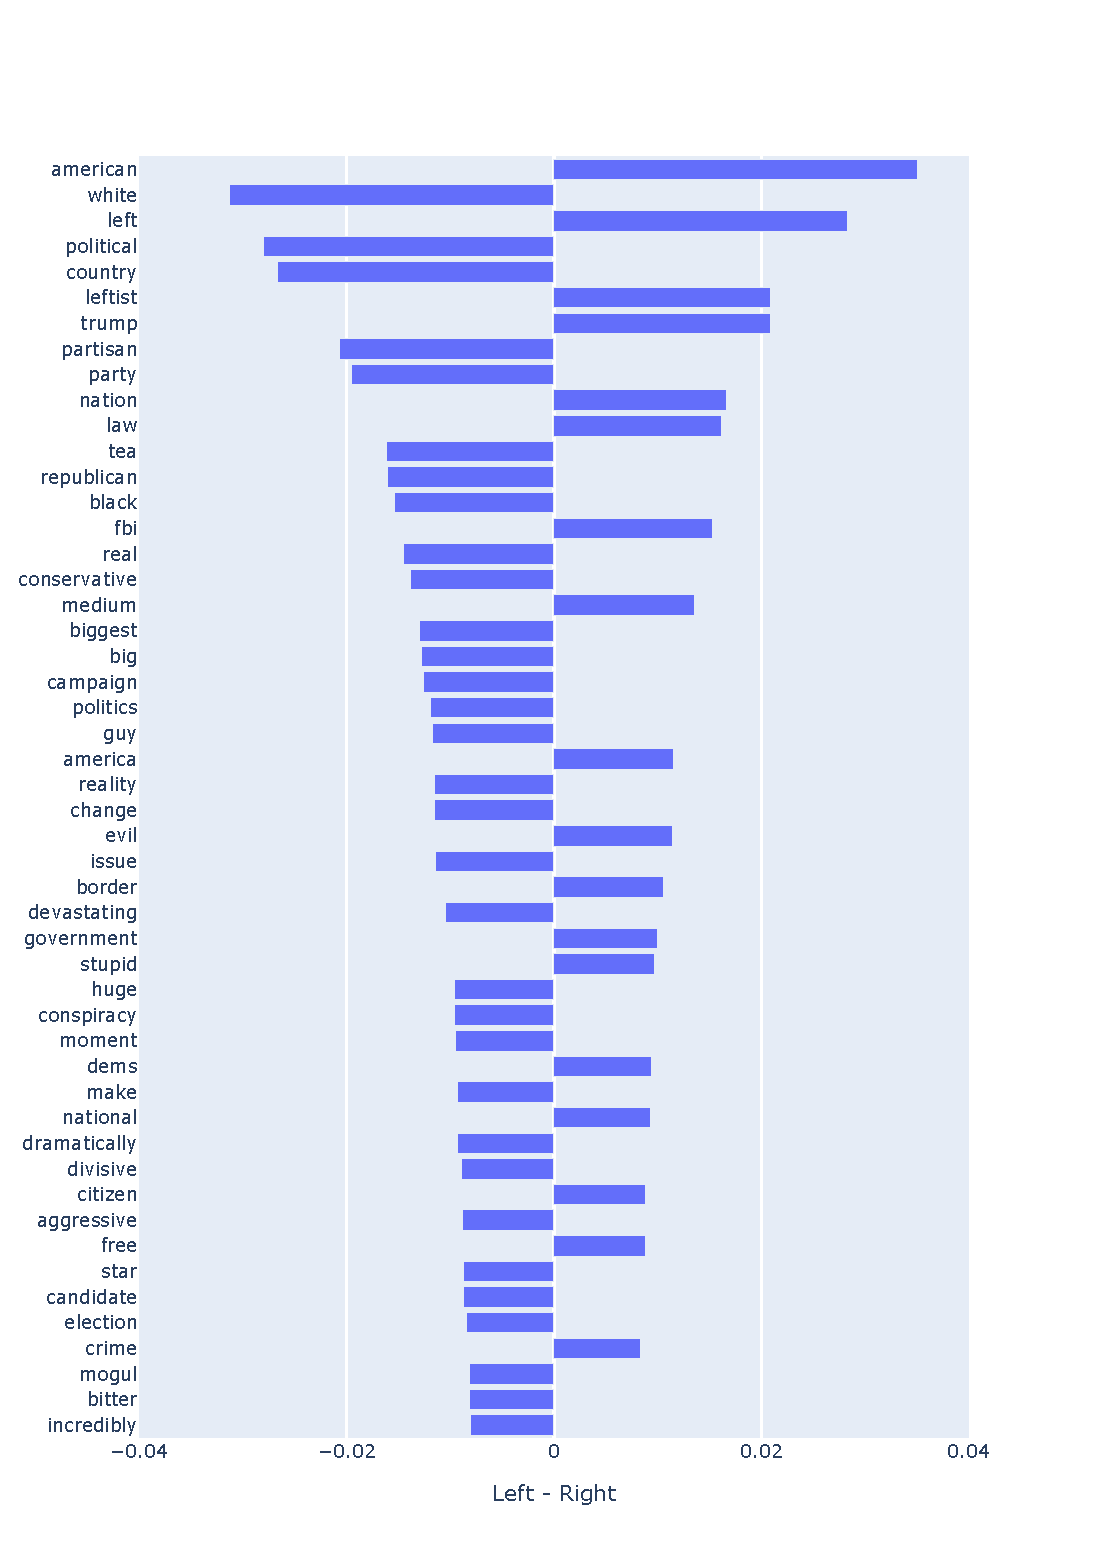
\includegraphics[trim={0 0 0 2cm},clip,width=\linewidth]{figures/baly_prop_tech_words_all_across_leaning_simple.pdf}
    \caption{Most distinguishable Propaganda terms across political leaning.}
    \label{fig:baly_prop_tech_words_all_across_leaning}
\end{figure}

Figure~\ref{fig:baly_prop_tech_words_all_across_leaning} shows the top 50 features (words) that have the highest difference between Left and Right TF-IDF scores.
On the horizontal axis, we can see the relative value of the difference on the Left-Right dimension.
% We did not remove stopwords because we are only dealing with some fragments of sentences that have been detected as propagandistic. For this reason the plot is showing some stopwords (e.g., ``a", ``of", ``the").\todoHA{Unclear why this stops you from removing stop-words}
From this plot we can recognise some propaganda terms.
For example ``american", ``left", ``leftist", ``nation", ``law" and ``border" that are more important for the Right. From~\citet{seargeant2020art} we know that the Right is using statements
% like ``we the people" which is a Right-leaning expression of populism.
that relate more with the identity  (american and nation) and protection  (law and border) of the country.
We also see the terms used to indicate the political opponents: ``leftist" and ``left".
Instead in the Left, we see terms such as ``white" and ``black" (emerging from articles about discrimination), ``partisan" ``republican" and ``conservative" (propaganda talking about the political opponents). 
% Then we notice some terms that are more related to the center: ``country", ``trump", ``nation", ``partisan", ``whistleblower", ``great".

\subsubsection{Propaganda Terms by Technique}
% TERM ANALYSIS PER TECHNIQUE
However, from this analysis, it is not clear how the terms found relate to the specific propaganda techniques. For this reason, we decide to perform again this analysis, but for each propaganda technique separately.
This means that we build the term frequencies for each of the 18 techniques, by collecting the terms that have been used in the specific technique by each leaning, and then building the TF-IDF feature separately and sorting again by the $(max - min)$ criterion.


\begin{table}[!htbp]
% \Rotatebox{90}{%
\resizebox{\textwidth}{!}{
    \centering
    \begin{tabular}{p{0.30\textwidth}|p{0.40\textwidth}|p{0.40\textwidth}|p{0.40\textwidth}}
        technique & Left & Center & Right \\
        \hline
         \texttt{Loaded\_Language} & in, that, into, self, devastating, hell & balk, more, very, whistleblower, hit, expose, batten, out, badgering, divisive, blast, circus, dramatic, chaos, severe & evil, blasted  \\
         \hline
         \texttt{Doubt} & just & trump, inadequate, transparency, grapple, will  & why, FBI, if \\
         \hline
         \texttt{Flag-Waving} & America, \textbf{white}, \textbf{black}, \textbf{life}, \textbf{society}  & democracy, state, security, family, value & \textbf{people}, \textbf{we}, \textbf{freedom}, \textbf{law}, \textbf{liberty} \\
         \hline
         \texttt{Name\_Calling/ Labeling} & party, \textbf{republican}, \textbf{right}, \textbf{conservative}, wing, real   & \textbf{partisan}, trump, witch, hunt, dems, whistleblower, innovator, dreamer, \textbf{centrist}, president, \textbf{democratic}, hoax  & \textbf{leftist}, racist, hating, law, \textbf{liberal}, \textbf{progressive}   \\
         \hline
         \texttt{Appeal\_to\_fear- prejudice} & \textbf{threat}, \textbf{climate}, difficult, death, die, disproportionate   & risk, backfire, credible, dangerous, confidence   & all, \textbf{destroy}, \textbf{attack}, fight, economically, racism, \textbf{invade}  \\
         \hline
         \texttt{Exaggeration/ Minimisation} & best, more, incredible, impossible, biggest, could, dramatically  & history, deadliest, big, unprecedented, life, degradation  & worst, absolutely, great, ever  \\
         \hline
         \texttt{Appeal\_to\_Authority} & medium, wisdom, \textbf{news}, know  & transparent, \textbf{intelligence}, official  & \textbf{note}, lie, open, \textbf{written}, accurate, fair, reflect   \\
         \hline
         \texttt{Reductio\_ad\_ hitlerum} & Stalinist, communism, partisan, & gestapo, nazi, eagle, religion, blame,   & hitler, Donald, tactic, propaganda, resurgent, science, death, gay \\
         \hline
         \texttt{Bandwagon} & find, common & say & taken, some, leave, future \\
         \hline
         \texttt{Black-and-White\_ Fallacy} & evolution, bible, proof, fall,  & impeachable, wall, good, strength, punch, military, justice, democratic, deal & my, live, change, amendment, senate \\
         \hline
         \texttt{Causal\_ Oversimplification} & plot, think & all, say, \textbf{reality}, reason, political & member, \textbf{leftist}, life, left  \\
         \hline
         \texttt{Obfuscation/ Intentional\_ Vagueness/ Confusion} & suggest, wrong, impossible, guide, evil, efficacy, anything & power, right, answer, excuse, truth, simply  & wing, meaning, rule, master, magic, fiction \\
         \hline
         \texttt{Red\_Herring} & love, pay, believe, anymore, like & & life, think, family, adulterous, America, republican, statement  \\
         \hline
         \texttt{Repetition} & jealous, blind, ObamaCare, bully, poison, lie  & more, temple, satanic, breathe & trump, obama, abiding, careless, law, pray, rigged, extremely  \\
         \hline
         \texttt{Slogans} & survival, fight, \textbf{matter}, \textbf{life}, face, \textbf{lives} & \textbf{America}, first, \textbf{great}, win, \textbf{make}, anchor, hero  & learn, amid, hearing, over, call, tax, race  \\
         \hline
         \texttt{Straw\_Men} & read, vote, opposition, trump & love, rule, poll & lie, news, god, want \\
         \hline
         \texttt{Thought-terminating\_ Cliches} & give, follow, lie  & wasting, time, drama & enough, break, evidence \\
         \hline
         \texttt{Whataboutism} & control, prison, & point, system, news, real, democrat, care  & apartheid, people, law, American, make, worse, contain \\
    \end{tabular}
}
    \caption{Most recognisable propaganda terms for each technique across leaning.}
    \label{tab:prop_words_by_technique_and_leaning}
\end{table}

With this method, we collect the most important words for each technique and leaning in Table~\ref{tab:prop_words_by_technique_and_leaning}.
%
As we can see, for each propaganda techniques there are different terms that are more or less important for each leaning.
While for some of these techniques, the terms shown by our analysis may not be very straightforward to interpret,
%are not very talkative,\todoHA{?} we can see
in some other cases the results are quite meaningful.
For example, in the \texttt{Name\_Calling/Labeling} technique we can see how the different political leanings address each others: the Right addresses the Left with the term \emph{leftist}, \emph{liberal} and \emph{progressive} and never with \emph{democrats} (term used instead by the Center). Instead, the Left addresses the Right with \emph{republican}, \emph{right} and \emph{conservative}.

Or for the \texttt{Flag-Waving} technique, we see how \emph{we the people} emerges from the Right, while the Left is more about \emph{white/black} and \emph{life/society}.
Also in the \texttt{Appeal\_to\_fear-prejudice}, we can see how thematically the Right is more recognisable for terms related to invasion/attack/destruction, while the Left emerges uniquely with \emph{climate}.
For the \texttt{Appeal\_to\_Authority}, the left has more use of the term \emph{news}, the Center instead with \emph{intelligence} and the Right with terms related to writing (\emph{written/note}).
And still in the \texttt{Slogans} technique, the center outlets emerges with the repetition of \emph{make America great again}, while the Left is repeating more the slogan \emph{Black lives matter}.

\subsection{Findings and Discussion}

The results from this experiment show that propaganda is used quite differently across the political leaning.
% We see significant\todoHA{Were the differences significant?}\todoAW{Very loaded word. Have you done a significance test?}
We are able to detect
differences both on aspects related to the amount of propaganda used, and on aspects related to the specific terms used.

% Quantities findings,  motivations and implications
Related to the quantities, we have the overall finding that we are detecting more propaganda on the articles coming from Right-leaning.
Left-leaning has slightly less propaganda and the Center has even less.
This relates with our expectation that propaganda is used more to express opinions on the extremes of the political spectrum, while in the center the discussions are kept a bit more neutral.
%\todoHA{What about the bias of the detection method to right propaganda?}
But as well, this could be a consequence of the detection method, that may be biased to recognise more easily propaganda from Right-leaning articles.
At the same time, we see that the sentiment analysis is showing similar distributions across the political leanings.
%\todoAW{Again, have you done a significance test?}

To go more in detail, we differentiated our analysis by considering the different propaganda techniques separately, and we have been able to find techniques that follow the general trend (\emph{U-shape}) across the leaning: \texttt{Loaded\_Language}, \texttt{Name\_Calling/Labeling}, \texttt{Exaggeration/Minimisation} and \texttt{Causal\_Oversimplification} with their polarising characteristics (extremes more, center less). Other techniques instead are more proper of one of the two leanings (\emph{triangular shape}): \texttt{Flag-Waving} and \texttt{Slogans} mostly on the Right. 


% Terms findings, motivations and implications
Instead, for the term analysis, we were able for some techniques to interpret the differences in the term importances by linking them to an understanding of the context of the dataset. For example, in \texttt{Flag-Waving} we recognised \textit{we the people} emerging from the Right-wing populism, or words from very frequently used slogans in the \texttt{Slogans} technique.
Recognising these features in the text can give a higher probability of belonging to one leaning than to the others.

% discussion
The quantity analysis provided quite useful insights over the preferred techniques from news sources coming from different political leanings. And the term analysis provided us with important terms that occur more in one leaning than in the others.
We have a much better understanding of how propaganda differs across the political spectrum.

% limitations
However, we have some limitations. By inspecting the samples, we observed in many cases that only parts of a technique were detected (boundaries not correctly captured, excluding terms that could be very useful for our term analysis).
% \todoHA{Examples?}
This is the own limitation of the current detection technique, which we took as it is and whose improvement is out of the scope of this thesis.

% link to next chapter
Furthermore, we would need to capture a bit more around the context of the propaganda techniques in order to understand what is their intent. We think that by analysing the topics of the articles more in details we could understand better the targets of propaganda and how propaganda is used as a mean to persuade in a certain direction about the topics. We will investigate the topics in the next Chapter~\ref{chap:topics}.

% link to next experiment
And as the last limitation, we extracted these insights, but we do not know to what extent they reflect in an immediate and definitive indication of the leaning of the articles.
The weightings of the TF-IDF show, in many cases, very similar scores. Therefore, it is unclear for now how easy or hard would it be to use these features to automatically recognise the leaning of one article. %(more in the next Subsection~\ref{ssec:ps_prop_leaning_classifier})
% it is not clear whether these features can be used to automatically differentiate between the propaganda of the left and the one from the right.
We experiment in this direction with the following Section~\ref{ssec:ps_prop_leaning_classifier}.


% \subsubsection{REMOVE: this subsubsection is about removing propaganda to increase similarity across leanings}
% \todo{This is describing another dubious experiment: removing propaganda to increase similarity of articles that refer to the same story. Instead here I want to talk about the analysis of propaganda acrosss spectrum}
% Instead of measuring the effect of removing the “framing” pieces on clustering algorithms, here we want to observe what is the effect on document similarity between different sources.
% Given articles from the left/center/right, we want to compare if there is a change in similarity when we remove sentiment and propaganda terms (e.g., articles are more similar than before).
% Hypothesis
% When removing propaganda/sentiment some political sides will be more similar to others. This is because the different parts are related to the propaganda/sentiment which is an added layer on top of the facts described.

% 1. Extraction of propaganda/sentiment
% Each article is analysed independently from the others, using the propaganda detection method and the sentiment lexicons.
% The percentages of words annotated with respect to the total number of words are computed for each article.
% 2. Grouping the percentages by political bias
% Considering the labels given by AllSides (left, lean-left, center, lean-right, right, mixed, not-rated), the average of sentiment-words-ratio, propaganda-words-ratio and both-ratio are computed. This gives an idea of how much of the articles from each political side is detected as sentiment-related or propaganda-related.

% % \begin{figure}[!htbp]
% %     \centering
% %     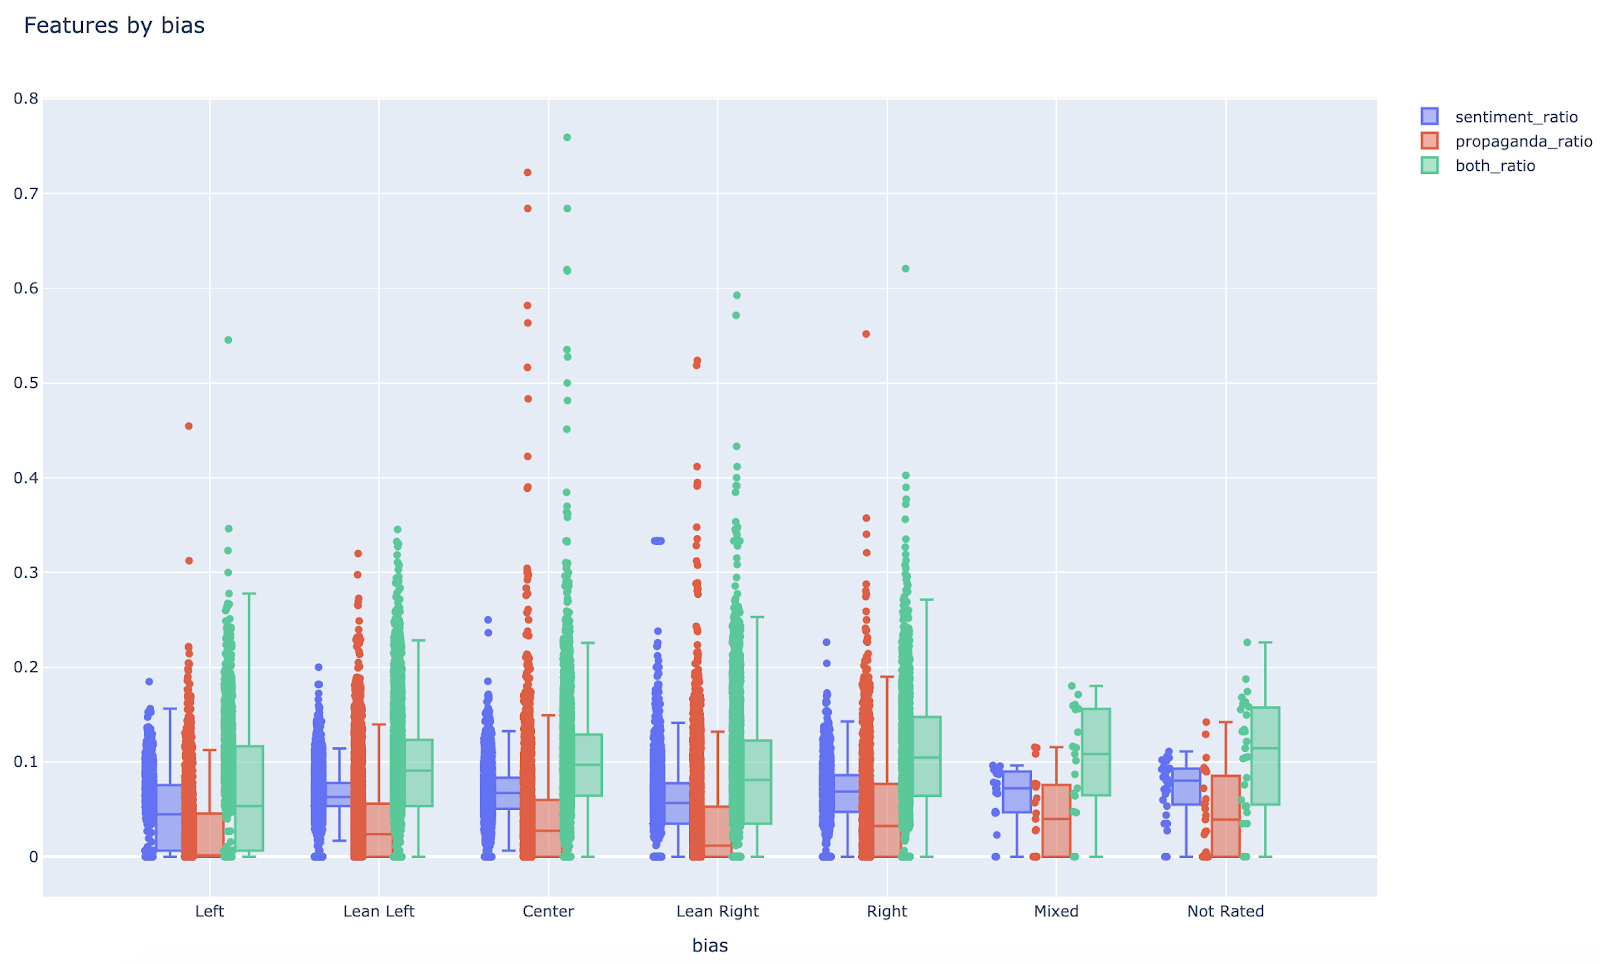
\includegraphics[width=\linewidth]{figures/4.3_prop_sent_across_leaning.png}
% %     \caption{Comparison of the detected sentiment and propaganda across the political leaning}
% %     \label{fig:prop_sent_across_leaning}
% % \end{figure}
% % \todo{Replace Figure~\ref{fig:prop_sent_across_leaning} with the one cleaned up, next in google docs}

% This plot in Figure~\ref{fig:prop_sent_across_leaning} is a quartile representation (with data points on the left of the boxes) which shows the distribution of the ratios computed. We can see that the average value (the line in the middle of the box) of “both\_ratio” is the highest for the “Right” side.
% From this plot we see that there are some very strange values (76\% of highlighted words in one article from the center). Looking at the details, this is an article from BBC which does not look so subjective. The problem is that from the full article, the scraping library only captured the sentence The statement says: ``It is an assault on UK sovereignty and any such use by a State party is a clear violation of the Chemical Weapons Convention and a breach of international law. It threatens the security of us all." which is annotated as almost everything propaganda. For other BBC articles, scraping manages to retrieve the full text without problems.

% There are also a lot of articles which have a percentage of 0\%. Looking at the distribution of the length of the documents, some documents, especially from some sources, have length=0 or a very short length (scraping the cookie disclaimer instead of the full article).
% For this reason a minimum length threshold has been set to cut out these problems: 150 tokens at least.

% This is the same plot, but with the filter on the minimum length.
% We can see that:
% The most annotated side is the Right
% The least annotated side is the Left
% Article from the Center do not contain less sentiment/propaganda (against assumption)
% There are less propaganda words than sentiment words



% 3. Creation of modified documents without the sentiment/propaganda parts
% As in the previous experiment (clustering), for each document other three documents have been created:
% Without propaganda words
% Without sentiment words
% Without propaganda and sentiment words
% Each document is embedded with two different methods:
% Universal Sentence Encoder
% TF-IDF (TODO dimensionality reduction, now it is a local TF-IDF to the cluster, see next point)


% 4. Comparing the articles about the same story
% Using the labels from AllSides, where articles are put together in groups of three items (usually one from the left, one from the center, one from the right), we compute the pairwise similarity matrix by using the embedded representations.
% For each cluster (provided by AllSides) we have 12 documents:
% Left-Full: the article from the left side, the full text
% Left-NoSent: the article from the left side, without sentiment words
% Left-NoProp: the article from the left side, without propaganda words
% Left-NoBoth: the article from the left side, without propaganda and sentiment words
% Center-Full: the article from the center side, the full text
% Center-NoSent: the article from the center side, without sentiment words
% Center-NoProp: the article from the center side, without propaganda words
% Center-NoBoth: the article from the center side, without propaganda and sentiment words
% Right-Full: the article from the right side, the full text
% Right-NoSent: the article from the right side, without sentiment words
% Right-NoProp: the article from the right side, without propaganda words
% Right-NoBoth: the article from the right side, without propaganda and sentiment words
% These articles are compared with a 12x12 matrix where the values are the similarity between the pair of docs.
% NOTE: at the moment, TF-IDF is computed locally to each cluster. I need to do the dimensionality reduction to be able to scale to more documents

% These similarities are then merged for all the AllSides clusters (being careful with the labels which can be different) and a final matrix is computed by doing an average of the matrices from the single clusters.
% The result is a 24x24 matrix (6 bias labels, not only left/center/right, multiplied with 4 variations of the same article).
% With this matrix it is possible to observe if, removing some parts of the articles, the similarity scores increase or decrease between different political sides.


% Results

% \todo{figures import}

% Observations:
% Within the rectangles on the main diagonal (yellow bright): comparison of the original articles with the modified ones generated from it:
% The removals are not changing the representations a lot: the scores are all quite high (minimum around 92% of similarity)
% The removal of propaganda parts is keeping the documents very similar to the original ones: average 98% similarity
% The removal of sentiment is changing a bit more the representation of the articles: minimum 93%, average 95%
% Increasing values between different biases (main diagonal of each block, see below):
% Usually similarity increases from Full article to noBoth
% Removing sentiment increases similarity (best scores)
% Removing propaganda decreases similarity a bit
% TODO: find a better way to represent this result. Just look at the main diagonals of each block, not so interesting to see the comparison between full articles and 

% Further improvements (TODOs):
% Propaganda/sentiment used by political sides by topic: break down by topic
% Propaganda types and sentiment scores by political sides: break down by fine-grained labels
% Verify correlation between propaganda:loaded\_language and sentiment. It is probably the same thing
% Improve visualisations of similarity changes (heatmap so big is confusing)
% Use dimensionality reduction and use a single TF-IDF model


% \todo{the rest (shapes...) goes in topic breakdown (next chapter)}


% Types of shapes (propaganda)
% (look at purple: propaganda)

% Blue is sentiment (+ and -) and purple is propaganda. 
% y axis in the fraction of terms marked as sentiment/propaganda.



\section{\statusgreen Political Leaning Classification using Propaganda Features}
\label{ssec:ps_prop_leaning_classifier}

% 5: political leaning classifier from propaganda features. Why
Here in this section, we take a different approach.
In the previous section, we saw how propaganda is slightly different considering the political leanings.
Taking from that result, we try to reverse the problem: using the features of propaganda extracted from the articles, can we automatically predict the leaning of an article?

This is what our second subquestion asks, RQ3.2: \emph{To what extent can we predict the political leaning of a news article by observing the propaganda it uses?}
More in detail, we want to see if it is possible to recognise the political leaning of articles from the:
\begin{enumerate}
    \item \emph{total amount} of propaganda found in the text (RQ3.2.1);
    %\item RQ2: Is it possible to recognise political leaning of articles from the \emph{amount of each propaganda technique} in the text?
    \item \emph{amount of each propaganda technique} in the text (RQ3.2.2);
    \item \emph{specific words belonging to propaganda techniques} in the article text (RQ3.2.3).
\end{enumerate}

% structure of next sections
The following subsection (\ref{ssec:ps_prop_leaning_classifier_motivations}) describes the motivations for conducting an experiment that uses propaganda to classify political leaning. Afterwards, we describe the general setup of the experiment (\ref{ssec:ps_prop_leaning_classifier_setup}), and then each of the three sub-research questions are addressed: quantity (\ref{ssec:ps_prop_leaning_classifier_total}), quantity by technique (\ref{ssec:ps_prop_leaning_classifier_techniques}), terms analysis (\ref{ssec:ps_prop_leaning_classifier_terms}).
For generalising better our results, we succesively present the results of the same analysis on the NELA-GT-2018 dataset (\ref{ssec:ps_prop_leaning_classifier_nela}).
This leads us into the last parts of this experiment, namely the discussions (\ref{ssec:ps_prop_leaning_classifier_discussion}) and conclusions (\ref{ssec:ps_prop_leaning_classifier_conclusion}).

% \todoHAinline{I'm struggling with this section. Maybe add subsections to help the reader to follow your thinking}
\subsection{Motivations}
\label{ssec:ps_prop_leaning_classifier_motivations}

% reasons
We have several reasons to think that using propaganda to classify political leaning could be useful.
% political leaning and propaganda are related; in other words, that propaganda changes across the political spectrum.
First of all, the results of our previous experiment that show differences in the quantity of propaganda techniques and also in the specific terms used.
If there are enough differences in the propaganda features considered, it means that we can use this to try to automatically recognise the political leaning.

% intro of TTO2020
There exist also reasons coming from the field of automated news analysis, where there is growing interest in understanding and classifying news articles based on their political ideology.
Various automated approaches have been recently proposed for the classification of articles with regards to political leaning~\citep{baly2020we} or credibility~\citep{horne2018assessing}. Others focused on capturing the usage of various propaganda techniques~\citep{da2019fine} or argumentation techniques~\citep{lippi2016argumentation}. However, the role that propaganda could play in automatically determining the leaning of articles has not been thoroughly investigated.
Propaganda is usually directly linked to the ideology of articles by having the ``intention of influencing people's opinions''.\footnote{\url{https://dictionary.cambridge.org/dictionary/english/propaganda}} To this end, we aim to better understand the relationship between propaganda analysis and the identification of political leaning of articles, simplified to three categories: \textit{Left}, \textit{Centre}, and \textit{Right}.

% Then, we also have a last reason.\todoHA{?} 
Lastly, we are also motivated by the analyses done in Chapter~\ref{chap:common_ground_search} and~\ref{chap:linguistic_persuasion}, where we observed the variations between multiple related articles.
%Both political leaning classification and propaganda analysis are types of political analysis.
% The point of contact between political leaning prediction and propaganda is that both are dealing with political analysis.
Also in this chapter we are considering articles that cover the same stories (as we have seen in the previous sections, we have triples of articles in the \texttt{baly} dataset)
Therefore, the facts that are being narrated are the same (except for the inclusion/exclusion of details). The main difference between an article from the left to one from the right is their point of view, with subjective and persuasive components.
Indeed, propaganda analysis is specifically focused on analysing this component of the articles.
As we discussed in Chapter~\ref{ssec:lit_layers_of_info}, we can think of news articles as a composition of two elements: the topical element (facts, entities, events) and the anti-topical element (how things are narrated, persuasion).
The topical elements need to be similar across the articles that narrate the same events (constraint of the dataset), and therefore we have a good setting for studying how the anti-topical elements vary across political leanings. 

% hypothesis
On top of this reasoning, we build our hypothesis that \emph{we can recognise the political leaning of an article by using the features provided by the propaganda analysis}.

% advantages
With respect to the State of the Art classifier presented in Section~\ref{ssec:ps_leaning_classifier}, whose results cannot be easily interpreted (black-box BERT-based classifier),
% \todoHA{why not?}
we could understand better why a certain article is classified as being left/right. We can get the relationship with the features and see which ones (quantities and terms) influenced more the classification outputs. 



Unlike previous work on political leaning detection, in this experiment we use the propaganda detection method (as in previous experiments, from \citet{da2019fine}) to identify the existence of propaganda and its type of techniques in given articles, and incorporate this information directly as additional features into the training and testing of the model.  

% what about sentiment?
We also experimented briefly with sentiment features, but after seeing the null results (and also the results from the previous experiment), we decided not to proceed with sentiment but only with propaganda.
% \todoHA{Where is this covered?} --> classifier based on sentiment features is not in this thesis, maybe commented out? or in notebooks
Therefore from here we switch our terminology from \emph{persuasion} (propaganda+sentiment) to \emph{propaganda}.




\subsection{Experimental Setup}
\label{ssec:ps_prop_leaning_classifier_setup}
% \todoAW{Experimental setup is important. This feels at quite the wrong level to me.}
% \todomargin{5.3, 5.4 and 5.5. each have different setup, so it is not possible to have all of them together}

We present here the experimental setup for this experiment, that is different from the ones of Section~\ref{ssec:ps_prop_leaning_across} and~\ref{ssec:ps_prop_leaning_imbalanced}.
As already mentioned, in this experiment we want to understand the impact of using propaganda features to estimate the leaning of news articles.

% General things before experiments
% Our experiments are designed to test the role of propaganda features in detecting the political leaning of articles. 
Therefore, we use the following steps to achieve this goal:
\begin{enumerate}
 %   \item ... ?collect data from AllSides ...
    \item Use the BERT-based political-leaning classifier baseline as described in the previous Section~\ref{ssec:ps_leaning_classifier}.
    % \todo{Why this baseline in particular?} 
    %~\citet{baly2020we} and apply it to the dataset to detect the political leaning of each article to reproduce the baseline results.
    \item Extract propaganda for each article using the tool from~\citet{da2019fine}.
    \item Add propaganda-related features to the BERT model, by injecting the values in the neural network using the (a) total presence of propaganda as a feature, (b) percentage of each propaganda technique, and (c) words that appear in the detected propaganda text.
    \item Train and test the model under different configurations with two splits, one totally random, and one less biased to media source.
    \item Compare our results with two baselines; the majority class (where the political leaning is assumed to be that of the most popular leaning in the dataset), and the results from our re-implementation of the model in step 1. %of \citet{baly2020we}.
\end{enumerate}

% \paragraph{Political Leaning Model}
% Our baseline is the same as described in the previous Section~\ref{ssec:ps_leaning_classifier}.

\begin{figure}[!htb]
    \centering
    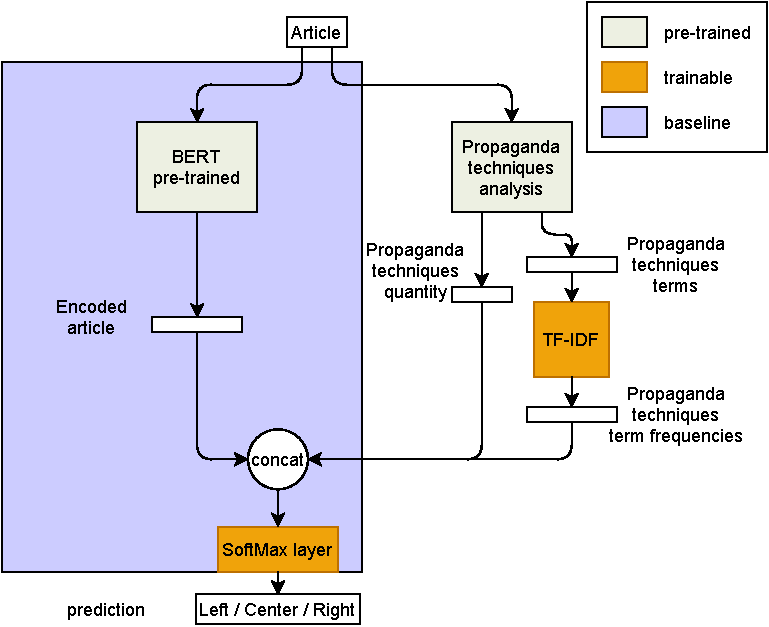
\includegraphics[width=\linewidth]{figures/methodology-Page-1.pdf}
    \caption{The architecture of the model to classify political leaning.}
    \label{fig:model_classifier}
\end{figure}

The setup for the classifier is represented in Figure~\ref{fig:model_classifier}. We can see on the left that we are encoding the articles with a pre-trained BERT model (cf. Section~\ref{ssec:ps_leaning_classifier}). On the right, instead, we are computing the propaganda features and then we inject them into the last layer of our neural network.


\subsubsection{Propaganda Features}


As mentioned earlier, for the propaganda analysis, we use the state of the art approach provided in~\citet{da2019fine}.\footnote{\url{https://huggingface.co/QCRI/PropagandaTechniquesAnalysis-en-BERT}} Their tool extracts 18 propaganda techniques. We apply this tool to the articles in our dataset to obtain these propaganda annotations. 
%and we gather the annotation for the articles in the dataset by using the official model released.
%API.\footnote{\url{https://app.swaggerhub.com/apis-docs/yifan2019/Tanbih/}}
%This model provides as result a set of spans from the text with a label corresponding to one of the 18 techniques.
% In addition to the propaganda techniques, we also run lexicon-based sentiment analysers to obtain a set of words loaded with sentiment with their polarity value (positive vs negative).
We use these annotations to calculate several numerical features that we employ in the following three sections to answer the three research questions introduced before.
%\begin{enumerate}
 %   \item the total quantity of propaganda (first
 %   \item the quantity of each propaganda technique
 %   \item the frequency of words that have been annotated for each propaganda technique
%\end{enumerate}

% The extracted features are then fed to a classifier that can be \sout{a SVM or} a Neural Network (single dense layer with softmax activation function).
% The train/test split for the 13k and 60k datasets is done with stratified split (to keep the proportion of L/C/R in the two splits): 90\% train, 10\% test.


% Our analysis workflow %model architecture we use 
% is depicted in Figure~\ref{fig:model_classifier}. 
Each article in the dataset is passed through the baseline BERT pre-trained models to calculate the baseline result, and through our models that incorporate the various propaganda features to calculate the results from our three different subquestions. %\todo{correct?} 
%Each article in the dataset is passed through either the baseline BERT pre-trained models, or the models that incorporate the various propaganda features. 
%The model The orange parts are being trained with the training set: the final SoftMax layer and the term-frequency analysis.

\subsubsection{Metrics}

We calculate the F1-macro and accuracy of the models and compare them with each other and with the baseline. % in search of any changes and improvements.%  we try to understand if there are some improvements for each of the three sections, and what is their statistical significance.
We also evaluate the significance of each added feature from the weight assigned to them %to each features 
by the classification model (the higher the weight, the more discriminative the feature is for Left/Centre/Right-leaning articles). %by looking at the weights of the models used, to understand what they learned.

%In some cases, 
We also combine the features given by each feature set, to see whether the addition of certain features helps to achieve higher classification accuracy. %values for the metrics. 
This combination is performed by concatenating the inputs to the SoftMax dense layer. It is not a combination of trained models, but it is a model that is trained and used on a combination of input features.


\begin{table}[!htbp]
    \centering
   \scriptsize
  %\small
    % \resizebox{\textwidth}{!}{
    \begin{tabular}{l|rr|rr}
        & \multicolumn{2}{c}{Random} & \multicolumn{2}{c}{Media} \\
        Model & F1-Macro & Accuracy & F1-Macro & Accuracy \\
        \hline
        \texttt{Majority} & 21.0286 & 46.0769 & 21.0286 & 46.0769 \\
        % \texttt{Baly-API} & 42.3355 & 43.8356 & 42.0523 & 43.6910 & 41.6863 & 41.7993 & & & & \\
        \texttt{Baly-baseline (0)} & $\star$56.4447 & $\star$58.6153 & 40.8647 & 46.2307 \\
        %\texttt{Baly-paper} (*) & 80.19 & 79.83 & 35.53 & 36.75 \\
        \hline
        \texttt{Prop-Total (1)} & 36.2966 & 42.3076 & 28.8285 & 41.5384 \\
        \texttt{Prop-Techniques (2)} & 36.7166 & 40.6153 & 33.0682 & 40.5384 \\
        \texttt{Prop-Total-Terms (3a)} & 42.0261 & 43.5384 & 41.5915 & 43.3076 \\
        \texttt{Prop-Techniques-Terms (3b)} & 42.4357 & 43.2307 & 40.8192 & 41.9230 \\
        % \texttt{Prop-words-BERT} (3) & 35.4718 & 48.2387 & 35.4718 & 48.2387 \\
        \hline
        \texttt{(0)+(1)} & 55.7786 & 57.7692 & \textbf{42.1847} & \textbf{47.5384} \\
        \texttt{(0)+(2)} & 54.9714 & 56.9999 & \textbf{42.4362} & \textbf{$\star$47.6153} \\
        \texttt{(1)+(2)} & 36.5217 & 40.4615 & 33.6202 & 41.0000 \\
        \texttt{(0)+(1)+(2)} & 55.2121 & 57.1538 & \textbf{42.2102} & \textbf{47.3846} \\
        \texttt{(0)+(3a)} & 54.6287 & 56.6923 & \textbf{41.9766} & \textbf{46.5384} \\
        \texttt{(0)+(3b)} & 54.8004 & 56.3076 & \textbf{41.9965} & 46.2307 \\
        \texttt{(3a)+(3b)} & 44.3506 & 46.3076 & \textbf{41.8725} & 44.3076 \\
        \texttt{(0)+(3a)+(3b)} & 53.2549 & 54.7692 & \textbf{42.0576} & 45.92307 \\
        \texttt{(1)+(2)+(3a)} & 42.0611 & 43.8461 & \textbf{42.5401} & 44.5384 \\
        \texttt{(0)+(1)+(2)+(3a)} & 54.0515 & 56.0769 & \textbf{42.2358} & \textbf{46.8461} \\
        \texttt{(1)+(2)+(3b)} & 44.3166 & 45.6153 & \textbf{41.9613} & 44.0000 \\
        \texttt{(0)+(1)+(2)+(3b)} & 45.6153 & 45.6153 & \textbf{41.9292} & 46.2307 \\
        \texttt{(1)+(2)+(3a)+(3b)} & 45.0456 & 47.2307 & \textbf{$\star$43.4564} & 45.9230 \\
        \texttt{(0)+(1)+(2)+(3a)+(3b)} & 53.6459 & 53.6459 & \textbf{42.5509} & \textbf{46.5384} \\
        
    \end{tabular}
    % }
    \caption{Results given by the different features and combinations of features.}
    \label{tab:results_prop_features_classifier}
\end{table}
% \todoHA{Table~\ref{tab:results_prop_features_classifier} p-values?}
% \todomargin{yes ideally, but need to compute for all the values}

Table~\ref{tab:results_prop_features_classifier} shows the results for all the three subsections below, to be able to compare the values all together.
In the first two rows, we can see the values for the two considered baselines (majority voting and BERT-based baseline).
Then, in the second group, we can see the results of the features considered on their own, without combination.
\texttt{Prop-Total} denotes the feature of the total quantity of propaganda, that is used to reply to RQ3.2.1 (Section~\ref{ssec:ps_prop_leaning_classifier_total}).
\texttt{Prop-Techniques} instead indicates the quantities of each propaganda technique, that are used as features to reply to RQ3.2.2 (Section~\ref{ssec:ps_prop_leaning_classifier_techniques}).
\texttt{Prop-Total-Terms} and \texttt{Prop-Techniques-Terms} relate to the term-based features, that are computed with TF-IDF of the propaganda words (first all together, then divided by propaganda technique), and are used to reply to RQ3.2.3 (Section~\ref{ssec:ps_prop_leaning_classifier_terms}).
% Baselines above, RQ3.2.1=\texttt{Prop-Total}, RQ3.2.2=\texttt{Prop-Techniques}, RQ3.2.3= (\texttt{Prop-Total-Terms} and \texttt{Prop-Techniques-Terms}).
Below, in the last group of the table, we can see various combinations of features that in some cases provide improvements over the baseline. \textbf{Bold} means that the score is higher than the baseline. The symbol $\star$ denotes the best result for the column.

\subsection{Total Quantity of Propaganda}
\label{ssec:ps_prop_leaning_classifier_total}


Our hypothesis behind RQ3.2.1 is that the total quantity of propaganda contained in an article helps to recognise its political leaning. 
% definition
To answer RQ3.2.1, we
% \todoHA{first?}\todomargin{no, only. more features in other subsections}
consider only the total amount of propaganda detected in each article. For each article, we calculate a single value to represent the percentage of propaganda text inside the article. %Using a percentage compensates for the varying lengths of articles.%These words are the one annotated as propaganda by \citet{da2019fine} (see Section \ref{sec:prop}).
% how it is computed
We use a percentage in order to be less biased and independent of the article size.
This value is computed for each article as the ratio between the number of words detected as propagandist (see previous Section \ref{ssec:ps_prop_leaning_across}) and the total number of words. For example, if an article has 600 words, and propaganda analysis annotated 30 of them as being propagandist, the value of the feature will be 5\%.  
% hypothesis
%The hypothesis is that by observing the total quantity of propaganda contained in an article, we can recognise its political leaning.
% stats
As we saw in the previous Section~\ref{ssec:ps_prop_leaning_across} in Figure~\ref{fig:prop_sent_across_leaning}, the distributions of the total quantity of propaganda is quite similar across political leaning, but it has lower values in the Center and higher values in the Right.
%Figure~\ref{fig:tot_quantity} shows how this value is distributed across Left, Centre and Right leaning articles. It appears that all three groups have a similar propaganda distribution. The Centre appears to have slightly less propaganda, and the Right sources have the most (could be due to propaganda bias as we highlight later in Section~\ref{sec:discussion}).%, especially looking at the dots that represent the outliers. 
% TODO better figure
 %Overall, the boxplot shows that the presence of propaganda is similar across the board.%, and the results in Table \ref{tab:results_prop_features_classifier} show that adding this feature lowers our classification accuracy. Hence %mostly overlap so this is a negative sign for our hypothesis.
%the answer to RQ3.2.1 is No, the mere presence of propaganda is insufficient to determining the political leaning of articles. 

% TODO: rename categories in plot to L/C/R
% \begin{figure}[!htb]
%     \centering
%     \includegraphics[width=\columnwidth]{figures/total_prop_data_condensed_mod.jpg}
%     \caption{Boxplot of the total amount of propaganda in Left, Centre and Right articles.}
%     \label{fig:tot_quantity}
% \end{figure}

% TODO move baseline considerations to section 3? When model will be shared by baly, this won't exist anymore
% Table~\ref{tab:results_prop_features_classifier} contains in the first group the baselines considered:

% \begin{itemize}
%     \item The \texttt{Majority} baseline, just providing the most common class as output, has quite low results and is considered here just as lower threshold on the other values.
%     \item \texttt{Baly-baseline}, being an emulation of what described in~\citet{baly2020we}, is still far from the 80\% results reported by the authors. For sure the source-code sharing from them that we are waiting will make the results improve
%     % \item \texttt{Baly-API} instead has much lower results that \texttt{Baly-baseline}, and therefore we can conclude that it is definitely not the implementation of the model described in~\citet{baly2020we}. It is coming from the same research group but we need to ask to the maintainers which results is it providing.
% \end{itemize}

\subsubsection{Results}
Table~\ref{tab:results_prop_features_classifier} shows the results of this first feature set under the name \texttt{Prop-Total}. The low values, just above the \texttt{Majority} baseline, indicate that the feature is unsuitable for determining which side an article belongs to. Both F1 and accuracy are below the values of \texttt{Baly-baseline} for both Random and Media splits. Even combining this feature with the baseline (i.e. adding propaganda percentage as features to the BERT model) does not provide an improvement, as shown by the row denoted by (0) + (1).



% % confusion matrix
% Looking at the confusion matrix of the 60k dataset in Figure~\ref{fig:total_prop_confusion_60k}, we can see that the model learned to predict the class with most articles, with a few exceptions that are classified as Right (probably the articles with a lot of propagandistic content, TODO compare with learned weights). A similar result can be seen in the 13k dataset. If instead we look at the balanced dataset, Figure~\ref{fig:total_prop_confusion_60k_balanced}, the models shifts to predicting random labels between Centre and Right.
% This means that, removing the shortcut~\citep{geirhos2020shortcut} of ``everything belongs to the Left'', the model cannot pick any relevant information from the feature described above.
% For the \texttt{baly} dataset instead,

\subsubsection{Confusion Analysis}

\begin{figure}[!htbp]
    \centering
    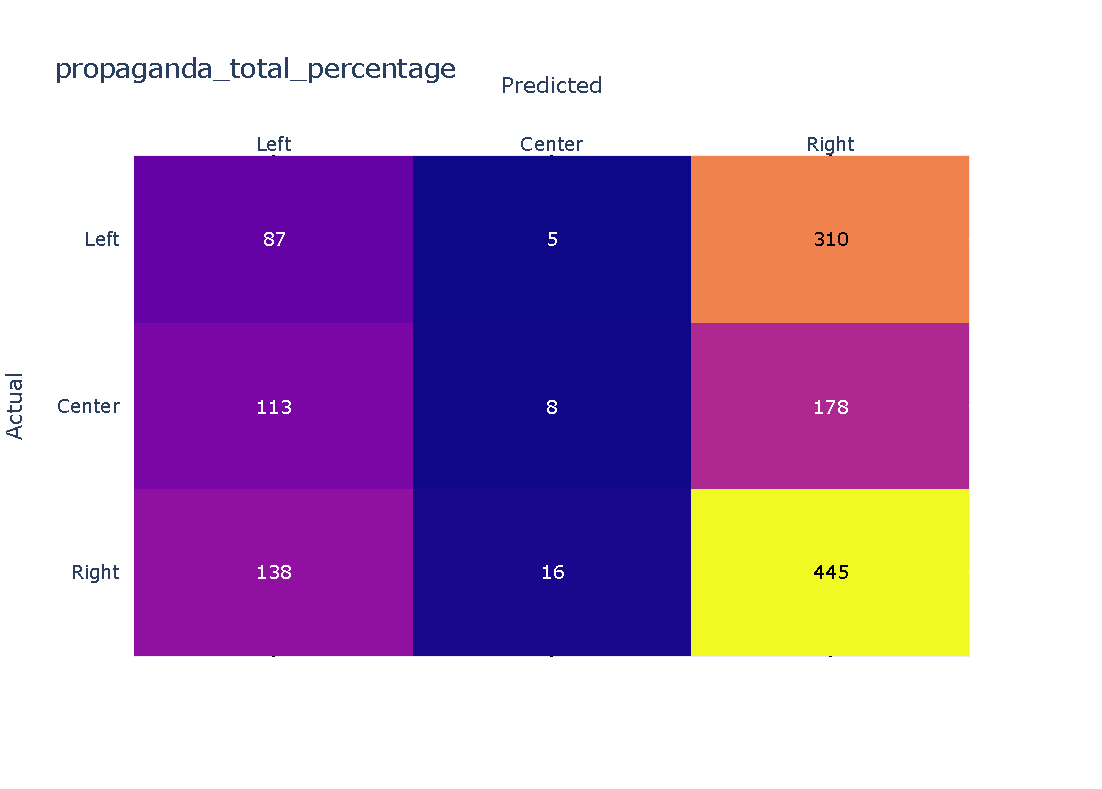
\includegraphics[width=0.75\linewidth]{figures/baly_media_confusion_matrix_propaganda_total_percentage.pdf}
    %\vspace{-1cm}
    \caption{Confusion matrix using the \texttt{Prop-Total} features (RQ3.2.1).}
    \label{fig:total_prop_confusion}
\end{figure}

The confusion matrix in Figure~\ref{fig:total_prop_confusion} shows that the classifier is introducing biased predictions towards the Right-leaning class. %From observing that in general right-leaning articles contain more propaganda overall (\texttt{Prop-Total} feature), the results are skewed right. 
This results in higher recall but lower precision for the Right class, and almost zero accuracy for the Centre label. 

In summary, the answer to RQ3.2.1 is: \textbf{the total amount of propaganda in an article does not seem to be a good indicator of the political leaning of an article}.

% provides a low result overall but a quite good F1 on the Right class.

% \begin{figure}[!h]
%     \centering
%      \begin{subfigure}[b]{0.45\linewidth}
%          \centering
%          \includegraphics[width=\linewidth]{figures/nodes_stratified_confusion_matrix_propaganda_total_percentage.pdf}
%          \caption{imbalanced 60k}
%          \label{fig:total_prop_confusion_60k}
%      \end{subfigure}
%     %  \hfill
%     \begin{subfigure}[b]{0.45\linewidth}
%          \centering
%          \includegraphics[width=\linewidth]{figures/nodes_stratifiedbalanced_confusion_matrix_propaganda_total_percentage.pdf}
%          \caption{Balanced 60k}
%          \label{fig:total_prop_confusion_60k_balanced}
%      \end{subfigure}
%      \\
%      \begin{subfigure}[b]{0.45\linewidth}
%          \centering
%          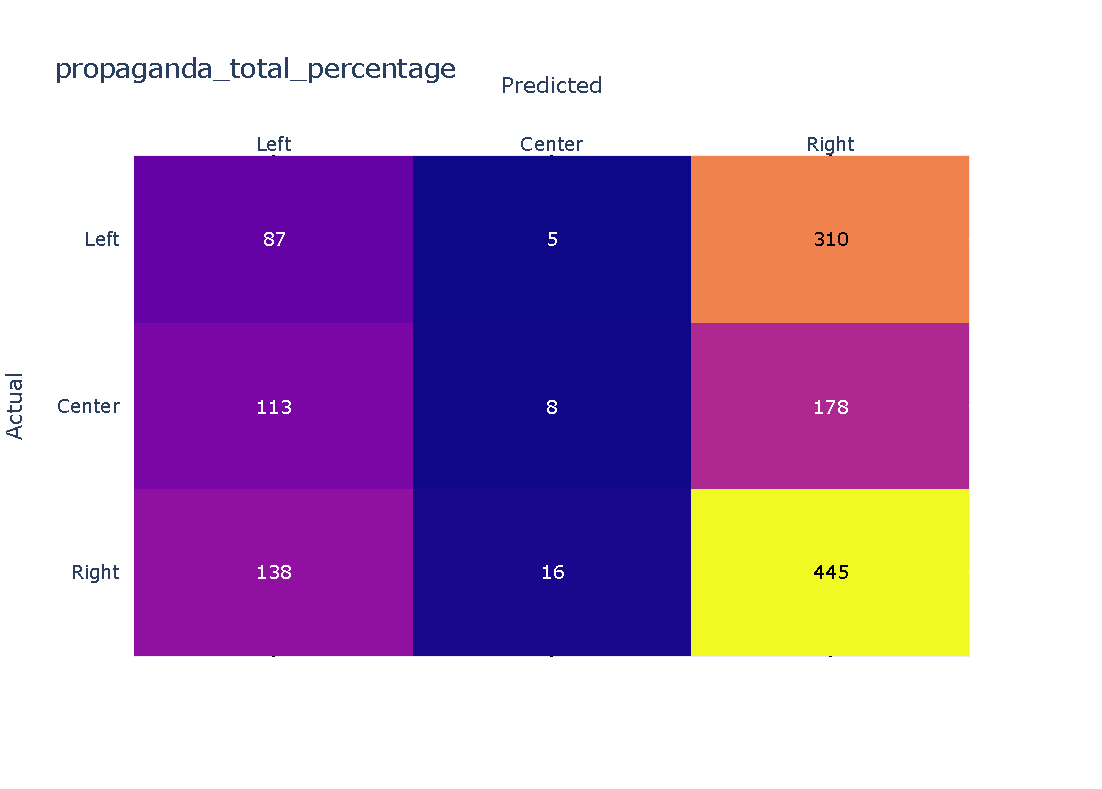
\includegraphics[width=\linewidth]{figures/baly_media_confusion_matrix_propaganda_total_percentage.pdf}
%          \caption{Baly}
%          \label{fig:total_prop_confusion_baly}
%      \end{subfigure}
%     \caption{Confusion matrix of the classifier using the features of \texttt{Prop-Total}.}
%     \label{fig:total_prop_confusion}
% \end{figure}



% TODO: double-check: if we explained the reasons for the classifier, inspecting the weights does not make sense
% % what the model learned:weights
% If we inspect the weights learned by the model in figure~\ref{fig:total_prop_weights}, the network simply learned that propaganda is mostly associated with the Left and not with the Center; the left is in the middle.
% This works well for the left-leaning articles (only 247 out of 2499 are mis-classified) while it does not produce good results for the other two political leanings.
% The decision based only on this feature acts in the following way:
% \begin{itemize}
%     \item if an article has low quantities of propaganda, it is put in the Left bucket (almost all the articles)
%     \item if an article has high quantities of propaganda, it is put in the Right bucket
%     \item no articles are put in the Center bucket (they should have negative quantities, according to the weights)
% \end{itemize}

% \begin{figure}[!h]
%     \centering
%     \includegraphics[width=\linewidth]{figures/total_prop_weights.png}
%     \caption{Weights of the classifier using only the total propaganda quantity: yellow means positive signal and purple means negative signal.}
%     \label{fig:total_prop_weights}
% \end{figure}

% significance

% The last row of Table~\ref{tab:q_60k} presents the combination of this feature with the baseline, which results in a small degradation of the baseline. This feature is not enough to recognise political leaning.


\subsection{Quantity of Particular Propaganda Techniques}
\label{ssec:ps_prop_leaning_classifier_techniques}

In this section, we test the hypothesis of RQ3.2.2, which is that the presence of particular propaganda techniques helps to determine the political-leaning of articles. 

%From the negative results to the first research question, we make another step to use more detailed features. 
Instead of relying on a single value representing the total quantity of propaganda, we now consider the amount of each propaganda technique to train the political-leaning classifier.
% The second step we take is to break the quantities of propaganda with respect of each one of the techniques.
The motivation behind is that a specific political leaning (e.g. Right-leaning) may be using one or more techniques more than others, and the classifier could pick these differences to perform its decisions.
This means that our feature vector is not a one-value vector but instead it is an 18-values vector, each one representing the amount of a specific propaganda technique (as also analysed in Section~\ref{ssec:ps_prop_leaning_across}).


We compute the word-based percentage of each technique inside each article. This means that the value for each technique is equal to the number of words belonging to it, divided by the total number of words in the document. A value of 1\% means that 1 out of 100 words in the document have been spotted as being part of the considered propaganda technique.
%We use a percentage, as in the previous case, in order to be independent on the article size.

% TODO: too small and messy figure
% \begin{figure}[!htb]
%     \centering
%     \includegraphics[width=\columnwidth]{figures/baly_prop_techniques_together.pdf}
%     \caption{Distribution of the amount of propaganda techniques in our dataset across Left (blue), Centre (green), and Right (red).}
%     \label{fig:prop_perc}
% \end{figure}

% data distribution
%To give an idea of the computed percentages, we grouped the articles according to their political leaning \textcolor{red}{as determined by AllSides}. 
As we have seen in the previous Section~\ref{ssec:ps_prop_leaning_across},  Figure~\ref{fig:prop_tech_details_across_leaning} was showing that the amount of propaganda techniques detected on this dataset is generally low. The most prominent one is the \texttt{Loaded\_Language} with an average word-based percentage of $1.5\%$.
As in the previous subsection, we observe that articles from the Centre appear to be using less most of the propaganda techniques, %, while Left and Right have higher percentages. This is expected given the overall propaganda use pattern found in the previous experiment.   %However, the difference seems minimal overall. 
but as we noted, there are some techniques which have different shapes (U-shape, triangular shape). Our hope is that an automated classifier is able to pick these different patterns and use them to differentiate the political leaning. 


% A similar procedure has been done for the sentiment analysis. First, sentiment words have been extracted by several lexicons (TODO list). In this way every sentiment-loaded term in the articles analysed is associated with its polarity value (positive or negative).
% Then with these annotations we extracted the percentage of positive tokens and negative tokens and used these as input features.


\subsubsection{Results}

% - Classifier with features: results and significance
We train the classifiers as the in previous case and obtain the result indicated by \texttt{Prop-Techniques (2)} in Table~\ref{tab:results_prop_features_classifier}. Although the results show improvement over the previous feature considered, they are still well below the best performing baseline. %This indicates that 
%As for the previous case, we have generally low scores, slightly improved from RQ3.2 on both splits.
The results show that (a) \texttt{Prop-Techniques} alone is insufficient to accurately detect the political leaning of articles (RQ3.2.2), and (b) when \texttt{Prop-Techniques} is added to \texttt{Baly-baseline} (line \texttt{(0)+(2)} in results table), it brings an improvement on the Media split for both the F1 and accuracy measures. 


%\begin{enumerate}
%    \item \texttt{Prop-Techniques} alone does not provide good results;
%    \item When \texttt{Prop-Techniques} is added to \texttt{Baly-baseline} in line (0) + (2), it does bring an improvement on the media split for both the F1 and accuracy measures.%, which is even bigger when added to the feature from the previous section.
    % \item When \texttt{Prop-Techniques} is added to \texttt{Baly-baseline} on the \texttt{Baly} dataset, it has a big improvement on both F1 and Accuracy
%\end{enumerate}

\subsubsection{Significance Test}

Given the improvements in some cases, we perform an additional test following the approach in~\citet{mcnemar1947note} 
to better understand the significance of these results. %if this is just a small effect or if it is something significant.
To perform this test, we build a contingency table by considering two arrays: the first shows when the \texttt{Baly-baseline} produced the correct result on the test set, and the second one shows when the line \texttt{(0)+(2)} (baseline+propaganda techniques quantity) produced the correct result on the Media split. The contingency table, therefore, is the 2x2 matrix as shown in 
% Table~\ref{tab:contingency} and 
Table~\ref{tab:contingency2}.

% \begin{table}[]
%     \centering
%     \begin{tabular}{c|c|c}
%         & \multicolumn{2}{c}{(0)+(1)+(2)} \\
%          & incorrect & correct \\
%          \hline
%         (0) incorrect & 2013 & 91 \\
%         (0) correct & 75 & 3868
%     \end{tabular}
%     \caption{Contingency table for 60k}
%     \label{tab:contingency}
% \end{table}

\begin{table}[]
    \centering
%    \scriptsize
\small
    \begin{tabular}{rr|c|c}
        & & \multicolumn{2}{c}{\texttt{(0)+(2)}} \\
         & & incorrect & correct \\
         \hline
        \multirow{2}{*}{\texttt{(0)}} & incorrect & 672 & 27 \\
        & correct & 10 & 591
    \end{tabular}
    \caption{Contingency table on Media splits.}
    \label{tab:contingency2}
\end{table}


% The first addition, when tested for significance with McNemar test with respect to the baseline, it provided a p-value=0.244 for 60k and p-value=0.608 for 13k. The values means that the contribution is not significant.
% Looking at the values of the contingency table, we can see that for the 60k dataset, adding the features from (1) and (2) made 91 elements of the test set to be correctly classified (misclassified instead from the baseline), but at the same time it brought other 75 elements with a correct label according to the baseline to be incorrectly classified.

% TODO move this in a more visible section, like final discussion? This applies to all the propaganda features
Using the predicted labels of the selected rows on the Media split (last two columns of Table~\ref{tab:results_prop_features_classifier}), the \texttt{(0)+(2)} against baseline resulted in a \textbf{p-value=$0.008$}, which means that the \textbf{improvement is significant}.
Remember that the \textbf{Media split is less biased than the Random split}, since in the Media split the sources of the articles in the test set are not overlapping with the sources of the articles in the training set. If we compare the Random vs Media split results, we can see that while the \texttt{Baly-baseline} drops significantly (more than 15\% F1 and 12\% accuracy), the models based on the features of propaganda have a much smaller drop in these measures (less than 8\% F1 and less than 1\% accuracy).
This means that our models with propaganda features are coping better with articles from ``new sources'' that are unseen in the training set. 
The improved generalisation abilities of this feature is perhaps what is driving the significant improvement described above. %can be seen when put in combination with the features of the baseline with the significant improvement described just above \textcolor{red}{(sentence unclear)}. 

\subsubsection{Confusion Analysis}

\begin{figure}[!htb]
    \centering
    %  \begin{subfigure}[b]{0.45\linewidth}
    %      \centering
    %      \includegraphics[width=\linewidth]{figures/nodes_stratified_confusion_matrix_propaganda_percentages.pdf}
    %      \caption{imbalanced 60k}
    %      \label{fig:prop_tech_confusion_60k}
    %  \end{subfigure}
    % %  \hfill
    % \begin{subfigure}[b]{0.45\linewidth}
    %      \centering 
    %      \includegraphics[width=\linewidth]{figures/nodes_stratifiedbalanced_confusion_matrix_propaganda_percentages.pdf}
    %      \caption{Balanced 60k}
    %      \label{fig:prop_tech_confusion_60k_balanced}
    %  \end{subfigure}
     \begin{subfigure}[b]{0.48\linewidth}
         \centering
         \includegraphics[width=\linewidth]{figures/baly_random_confusion_matrix_propaganda_percentages-small.pdf}
         \caption{Baly random.}
         \label{fig:prop_tech_confusion_baly_random}
     \end{subfigure}
    %  \hfill
    \begin{subfigure}[b]{0.48\linewidth}
         \centering 
         \includegraphics[width=\linewidth]{figures/baly_media_confusion_matrix_propaganda_percentages-small.pdf}
         \caption{Baly media.}
         \label{fig:prop_tech_confusion_baly_media}
     \end{subfigure}
    \caption{Confusion matrix using the features of \texttt{Prop-Techniques} (RQ3.2.2).}
    \label{fig:prop_tech_confusion}
\end{figure}


% confusion matrix
Figure~\ref{fig:prop_tech_confusion} is the confusion matrix for the classifier using the \texttt{Prop-Techniques} feature alone. It shows that the situation is very similar to the previous Subsection~\ref{ssec:ps_prop_leaning_classifier_total}. More articles are predicted as being Right-leaning with respect to the other two classes. %, because it is the most represented class.
% From the imbalanced situation in \ref{fig:prop_tech_confusion_60k}, where the articles were generally predicted to be Left leaning, the subfigure \ref{fig:prop_tech_confusion_60k_balanced} shows that after the correction most of the articles are classified on the Centre.
If we compare the subfigures~\ref{fig:prop_tech_confusion_baly_random} and~\ref{fig:prop_tech_confusion_baly_media}, we see that they are quite similar (F1 and accuracy are very similar too). The only difference is that the Media split predictions are more Right-leaning biased, resulting in lower local F1 for Left and Centre.

\subsubsection{Feature Importance Analysis}

\begin{figure}[!htb]
    \centering
    \includegraphics[width=\linewidth]{figures/nodes_stratifiedbalanced_weights_propaganda_percentages-small-simple.pdf}
    \caption{Weights for the \texttt{Prop-Techniques} features on the balanced dataset.}
    \label{fig:prop_tech_weights}
\end{figure}

% features learned
To understand what the model has learnt, we investigate the weights assigned by the neural layer part of the model.
The values are retrieved from the neural network by analysing the weights of the SoftMax layer described before.
For each feature, we have three weightss that respectively affect the probabilities assigned to the three output classes (Left, Center, Right).
From these three weights, we compute the difference between the ones for the Right class and the one for the Left class. This computed value represents the association between the specific technique and the output leaning. 
We can see in Figure~\ref{fig:prop_tech_weights} the associations learned by the model for the eighteen techniques considered.
Positive values correspond to higher weights for the Right class, while negative values mean that the classifier recognises the appearance of the technique as a sign of being from the Left.

Right is associated with some propaganda techniques (e.g. Slogans and Reductio ad Hitlerum), while the Left is more associated with other techniques (e.g. Exaggeration/Minimisation and Thought-terminating cliches).
% The Centre is generally associated by the model with an absence of all  propaganda techniques.
It is important to note that given the low F1 score of 40\%, the weight assigned by this model for each propaganda technique is only indicative. %does not not represent the ground-truth. 
The model is simply overfitting on the features provided.

%We need to specify that the weights observed do not directly represent the amount of each technique in the corpus. They represent only values that the neural layer assigned as internal weights to optimise the loss on the training set. If the models were having very nice performances we could say that what the model learned is correct, while in this case with values of F1 around 40\% the features learned do not represent quite well the political leaning.



The conclusion for this subquestion RQ3.2.2 is that \textbf{the amount of each propaganda technique is not enough on its own to accurately recognise the political leaning of an article, but when combined with the baseline features produces a significant improvement}.


\subsection{Terms of Propaganda}
\label{ssec:ps_prop_leaning_classifier_terms}

% TODO: keep together propaganda spans instead of tokenizing (e.g., "")
%Given the results of the two previous experiments, and the room for improvement that is left above the scores shown, we want to have a better understanding of the differences between the propaganda coming from multiple political sides.
Following on from the previous two subquestions, we now aim to reach a better understanding of the differences between how propaganda is portrayed in articles belonging to each political side.
We need to go beyond the quantification of detected propaganda techniques (RQ3.2.1 and RQ3.2.2), and investigate the chosen terminology for expressing these propaganda techniques in articles belonging to Left, Right, or Centre (RQ3.2.3). %how the techniques differ across the political spectrum with regards to used language. 
% to recognise political leaning given by the previous sections, the idea is to take a look at the specific terms picked up by the propaganda analysis. Not only quantity, but which words belong to each technique.

%To this end, the RQ3.2.3 considers as features the terms that are picked as part of the propaganda techniques.
The hypothesis is that, even though propaganda techniques are used with similar percentages (as learnt from the first two feature sets), the choice of words and their frequency differ between different-leaning articles, which can improve their classification. 
%there are some specific words that are used by opposing leanings that are used with different frequency.
%
In this third part, we proceed with the analysis of terms in two different ways:
\begin{itemize}
    \item (3a) all the propaganda words taken together: non-propaganda annotated words are filtered out. The classifier will then use the remaining propaganda words to learn any differences between political leanings. 
    %this acts as an attention mask between the classifier and the articles, filtering out the words that are not propagandist. The classifier will then use the propaganda words to learn any difference between political leanings. 
    \item (3b) propaganda words grouped by propaganda technique: there are 18 groups, one for each propaganda technique. The classifier will use the words, grouped by the technique to which they belong, to recognise the political leaning.
\end{itemize}

While the objective of (3a) is to learn distinctive propaganda terms, (3b) instead focuses on the terms of the 18 individual techniques (e.g. Slogans from the Right might contain different words from the Slogans from the Left).
% \todoHA{You have to add examples whenever and wherever you can}

To obtain the feature vectors of the propaganda words, we use TF-IDF 
because its numerical values directly represent single terms. Instead with other embedding methods (e.g., GloVe~\citep{pennington2014glove}, FastText~\citep{joulin2016fasttext}) this correspondence with single terms would be more difficult to extract. By considering the features which get assigned the biggest values in the final SoftMax layer, we can directly say which terms are the most discriminative for the task of political leaning classification.
% since it is easier to link the results to specific terms: the TF-IDF weights that vary the most between political sides are labelled with their feature name (term). 
% the results produced can be easily interpreted. Using State of the Art word embeddings could provide better results but it would be more difficult to understand the importance of specific terms.

\subsubsection{Results}
% results

The row of Table~\ref{tab:results_prop_features_classifier} with the label \texttt{Prop-Total-Terms (3a)} refers to the TF-IDF features computed by only using the propaganda terms, without differentiating between the different techniques.
This row has significantly better results than \texttt{(1)} and \texttt{(2)} on both splits, but only outperform the \texttt{Baly-baseline}  on the Media split in F1. %(not accuracy though). 

On the other hand, the feature \texttt{Prop-Techniques-Terms (3b)} refers to splitting the propaganda terms into the 18 groups and then computing the TF-IDF features on each group separately. The results of this feature set are generally a few decimal points below \texttt{(3a)}.


% % confusion matrix
% To better understand this performance, %where this feature is working and where it is making the prediction fail, 
% we can take a look at Figure~\ref{fig:terms_confusion}, which shows the predictions of the models trained with the features in (3a).
% %TODO: SUBFIGURE DIFFERENCE a/b is NOT RELEVANT. 
% \textcolor{red}{unclear what we learn from this particular confusion matrix. either explain or remove it.  }

% On the imbalanced dataset, the class that has more errors is the Center and the Left side is the most correct, while in the balanced the main diagonal is able to emerge a bit from the other values. On the balanced dataset there is a small bias of the model to say the articles are Right leaning.
% The results and confusion matrix are very similar between the feature (3a) and (3b).

% \begin{figure}[!h]
%     \centering
%      \begin{subfigure}[b]{0.45\linewidth}
%          \centering
%          \includegraphics[width=\linewidth]{figures/nodes_stratified_confusion_matrix_propaganda_tf_idf.pdf}
%          \caption{imbalanced 60k}
%          \label{fig:terms_confusion_60k}
%      \end{subfigure}
%     %  \hfill
%     \begin{subfigure}[b]{0.45\linewidth}
%          \centering 
%          \includegraphics[width=\linewidth]{figures/nodes_stratifiedbalanced_confusion_matrix_propaganda_tf_idf.pdf}
%          \caption{Balanced 60k}
%          \label{fig:terms_confusion_60k_balanced}
%      \end{subfigure}
%     \caption{Confusion matrix of the classifier using the features of \texttt{Prop-Techniques-Terms} (3a).}
%     \label{fig:terms_confusion}
% \end{figure}

% NON-RELEVANT DIFFERENCE BETWEEN A and B 
% \begin{figure}[!htb]
%     \centering
%      \begin{subfigure}[b]{0.48\linewidth}
%          \centering
%          \includegraphics[width=\linewidth]{figures/baly_random_confusion_matrix_propaganda_tf_idf-small.pdf}
%          \caption{Random splits}
%          \label{fig:terms_confusion_random}
%      \end{subfigure}
%     %  \hfill
%     \begin{subfigure}[b]{0.48\linewidth}
%          \centering 
%          \includegraphics[width=\linewidth]{figures/baly_media_confusion_matrix_propaganda_tf_idf-small.pdf}
%          \caption{Media splits}
%          \label{fig:terms_confusion_60k_media}
%      \end{subfigure}
%     \caption{Confusion matrix of the classifier using the features of \texttt{Prop-Techniques-Terms} (3a).}
%     \label{fig:terms_confusion}
% \end{figure}

\subsubsection{Feature Importance Analysis}

% - Classifier with features: features learned?
% BERT: no interpretation?
% TF-IDF weights? TODO
To better understand what the model has learnt, we take a closer look at the neural layer weights assigned to the TF-IDF features.
Figure~\ref{fig:terms_weights_3a} shows the 30 most important terms derived from the weights assigned.
We can see the term ``fit'' emerging as a very representative term of the Centre-propaganda, the terms ``establishment'' and ``suggest'' being significant for the Left, and the terms ``threaten'', ``spread'' and ``prevent'' are mostly associated with the Right-leaning propaganda.


% TODO: make clearer distinction between propaganda label and word
\begin{figure}[!htb]
    \centering
     \begin{subfigure}[b]{\linewidth}
         \centering
         \includegraphics[width=0.75\linewidth]{figures/baly_media_weights_propaganda_tf_idf-small.pdf}
         \caption{\texttt{Prop-Total-Terms}(3a): propaganda terms.}
         \label{fig:terms_weights_3a}
     \end{subfigure}
    %  \hfill
    \begin{subfigure}[b]{\linewidth}
         \centering 
         \includegraphics[width=0.75\linewidth]{figures/baly_media_weights_propaganda_techniques_tf_idf-small.pdf}
         \caption{\texttt{Prop-Techniques-Terms} (3b): propaganda terms together with their propaganda technique.}
         \label{fig:terms_weights_3b}
     \end{subfigure}
    \caption{The 30 most important terms learned by the classifier.}
    \label{fig:terms_weights}
\end{figure}
% \todo{barcharts like in \ref{fig:baly_prop_tech_words_all_across_leaning}} --> problem with features and feature names missing / ugly

In Figure~\ref{fig:terms_weights_3b}, we consider each propaganda technique separately. The most discriminating word is ``free'' belonging to the \texttt{Slogans} technique, which has the highest weight for the Right, and the lowest value for the Left. Similar values have the term ``courageous'' (Repetition), ``washington'' (Name Calling) and ``matter'' (Slogans). Terms such as ``idea''(Doubt) and ``support'' (Flag-Waving) instead are mostly associated with the Left-leaning propaganda.

Further investigation is needed to better capture what each of these words means in the context they are used, to determine how to improve on this term analysis.% could be improved and be able to distinguish political sides more effectively.

With the current analysis, we can say that \textbf{the answer to RQ3.2.3 is that the specific propaganda words can only marginally help to classify the political leaning. Using the terms of propaganda we achieve a very similar score to the baseline (rows indicated with \texttt{(3a)} and \texttt{(3b)}), and when added to the baseline features, it helps to achieve a small (but not significant, \textit{p-value=0.657}) improvement}. % NOT SIGNIFICANT IMPROVEMENT: p-value=0.657


\subsection{\statusgreen Reproduction on \texttt{NELA-GT-2018} Dataset}
\label{ssec:ps_prop_leaning_classifier_nela}

% \todo{take from experiment 6 document}
% % 6: classifier (propaganda → leaning) on other datasets

% What: this experiment was reproduced with NELA dataset (MBFC for leaning of the sources)

% Why: The results have similar scores. The significance test is passed but we question whether the results would generalise to other datasets.
% check with other datasets if this behaviour generalises

We have seen in the previous sections that the results of the classifier based on the propaganda features are not setting a big difference in the F1 scores. On the media splits, we managed to increase by a few percentage points (2.59\% F1, 1.38\% accuracy), while on the random splits the baseline still provides the best results.
The feature combination \texttt{(0)+(2)} (baseline and quantity of propaganda techniques), when tested for with McNemar test, resulted significant (p-value $=0.008$).
But we still question whether the results, with such a small margin (F1 and Accuracy) would generalise to other datasets.

For this reason, in this subsection, we take the \texttt{NELA} dataset from Section~\ref{app:nela_processing} and we perform the same analysis. In specific, we test on the built subsets denoted with \texttt{NELA-Random-Imbalanced}, \texttt{NELA-Random-Balanced}, \texttt{NELA-Media-Imbalanced} and \texttt{NELA-Media-Balanced}.


The only difference in the experimental setup is that here we are performing a 5-Folds cross-validation instead of a simple train-test.
As discussed in the Appendix, this gives more generalisable results and is less dependent on which articles have been chosen for the test set (particularly when we are using the media splits).

For computing the F1 and accuracy metrics, we accumulate over the 5 folds the values of the true and predicted labels.

\begin{table}[!htbp]
    \centering
   \scriptsize
  %\small
    \resizebox{\textwidth}{!}{
    \begin{tabular}{l|rr|rr|rr|rr}
        & \multicolumn{2}{c}{\texttt{Random-Imbalanced}} & \multicolumn{2}{c}{\texttt{Random-Balanced}} & \multicolumn{2}{c}{\texttt{Media-Imbalanced}} & \multicolumn{2}{c}{\texttt{Media-Balanced}} \\
        Model & F1-Macro & Accuracy & F1-Macro & Accuracy & F1-Macro & Accuracy & F1-Macro & Accuracy \\
        \hline
        \texttt{Majority} & 21.5632 & 47.8086 & 16.6666 & 33.3333 & 21.5632 & 47.8086 & 16.6666 & 33.3333 \\
        % \texttt{Baly-API} & 42.3355 & 43.8356 & 42.0523 & 43.6910 & 41.6863 & 41.7993 & & & & \\
        \texttt{Baly-baseline} (0) & 69.2076 & 71.2211 & 70.9808 & 70.8977 & 45.1628 & 50.5888 & 46.2165 & 46.0180 \\
        %\texttt{Baly-paper} (*) & 80.19 & 79.83 & 35.53 & 36.75 \\
        \hline
        \texttt{Prop-Total (1)} & 21.5632 & 47.8086 & 29.5603 & 35.2938 & 21.7242 & 47.8372 & 32.4953 & 33.0485 \\
        \texttt{Prop-Techniques (2)} & 25.6280 & 47.8404 & 38.4605 & 39.7791 & 24.2318 & 46.1973 & 36.3153 & 37.5012 \\
        \texttt{Prop-Total-Terms (3a)} & 41.3193 & 49.6682 & 41.8435 & 42.3996 & 37.0437 & 45.3760 & 36.8032 & 36.8067 \\
        \texttt{Prop-Techniques-Terms (3b)} & 38.3522 & 50.3530 & 39.3319 & 41.0597 & 35.3254 & 47.3457 & 35.6495 & 35.8892 \\
        % \texttt{Prop-words-BERT} (3) & 35.4718 & 48.2387 & 35.4718 & 48.2387 \\
        \hline
        \texttt{(0)+(1)} & \textbf{69.2085} & \textbf{71.2271} & \textbf{70.9899} & \textbf{70.9057} & 45.1531 & \textbf{50.6024} & \textbf{46.2288} & \textbf{46.0346}  \\
        \texttt{(0)+(2)} & \textbf{69.2905} & \textbf{71.2991} & \textbf{71.0331} & \textbf{70.9510} & \textbf{45.1835} & \textbf{50.6412} & \textbf{46.3481} & \textbf{46.1550} \\
        \texttt{(1)+(2)} & 25.7629 & 47.8299 & 38.5816 & 39.8064 & 24.4286 & 46.2459 & 36.2956 & 37.1280 \\
        \texttt{(0)+(1)+(2)} & \textbf{$\star$69.2994} & \textbf{$\star$71.3019} & \textbf{$\star$71.0358} & \textbf{$\star$70.9529} & \textbf{$\star$45.1998} & \textbf{$\star$50.6524} & \textbf{46.3457} & \textbf{46.1517} \\
        \texttt{(0)+(3a)} & 65.7886 & 68.5003 & 68.5460 & 68.4628 & 44.7002 & 49.4820 & 46.1694 & 46.1916 \\
        \texttt{(0)+(3b)} & 66.1823 & 68.7194 & 68.5074 & 68.4349 & 45.0300 & 49.8181 & \textbf{46.4617} & \textbf{46.4431} \\
        \texttt{(3a)+(3b)} & 41.4558 & 49.5529 & 42.5407 & 42.6677 & 37.0566 & 45.1370 & 36.5396 & 36.5419 \\
        \texttt{(0)+(3a)+(3b)} & 65.0796 & 67.8463 & 67.4347 & 67.3705 & 44.4791 & 49.1030 & 45.9924 & 46.0147  \\
        \texttt{(1)+(2)+(3a)} & 41.6843 & 49.9994 & 42.2068 & 42.7608 & 36.9627 & 45.4902 & 36.4236 & 36.4208   \\
        \texttt{(0)+(1)+(2)+(3a)} & 65.7779 & 68.4993 & 68.5715 & 68.4921 & 44.8164 & 49.5117 & \textbf{46.2871} & \textbf{46.3227}  \\
        \texttt{(1)+(2)+(3b)} & 38.8414 & 50.4508 & 39.6869 & 41.3132 & 35.7261 & 47.4435 & 35.8977 & 36.0895  \\
        \texttt{(0)+(1)+(2)+(3b)} & 66.1066 & 68.6778 & 68.5074 & 68.4376 & 45.0148 & 49.8192 & \textbf{$\star$46.6062} & \textbf{$\star$46.6054} \\
        \texttt{(1)+(2)+(3a)+(3b)} & 41.7298 & 49.8055 & 42.6323 & 42.7555 & 36.8644 & 45.1150 & 36.7762 & 36.8838 \\
        \texttt{(0)+(1)+(2)+(3a)+(3b)} & 65.0692 & 67.8439 & 67.4353 & 67.3718 & 44.5016 & 49.1166 & 46.05313 & 46.0858  \\
        
    \end{tabular}
    }
    \caption{Results NELA.}
    \label{tab:results_prop_features_classifier_nela}
\end{table}

Table~\ref{tab:results_prop_features_classifier_nela} shows the results. We denote also in this table with \textbf{bold} the scores that are higher than the baseline, while the $\star$ symbol means indicates the highest score for the column.

\subsubsection{Results}

% Result: similar behaviour
First of all, if we consider the macro categories of baseline / propaganda features / combinations (the main three groups of rows, separated by horizontal lines), we have a similar behaviour with the \texttt{baly} dataset. The propaganda features alone are not enough to go beyond the initial results from the baseline. However, when the features are combined together with the baseline features, we see an increase of the F1-Macro and Accuracy scores.
But in this case, for each of the 4 splitting methods, we have that some feature combinations are better than the baseline.

% random vs media
Comparing Random vs Media splits, we have confirmed also with this dataset that the Media splits are harder to learn. Having the articles from each media source appear only or in the training set or in the testing set, the model finds at prediction time only news articles that come from unknown sources and whose linguistical style is unknown. Therefore, it cannot use the shortcut of simply recognising the news source style and then output the corresponding leaning.

Also here we see that the propaganda features considered on their own have a smaller gap with respect to the baseline in the media splits (less than 10\% in the media splits, almost 30\% in the random splits).
% \todoAW{Be consistent in your precision. Why is this "less than 10\%", but later you have "0.1292 F1"?}
This means that they are able to generalise better with unseen news sources.

These improved generalisation abilities over the media splits, also reflect on the improvements over the baseline:
\begin{itemize}
    \item with \texttt{Random-Balanced}, the delta between \texttt{(0)+(1)+(2)} and \texttt{(0)} is: 0.05\% for both F1 and Accuracy; % , 0.0552\%
    \item with \texttt{Media-Balanced}, the same delta is: 0.12\% F1, 0.13\% Accuracy; % 0.1292 and 0.1337
    \item the best result of \texttt{Media-Balanced} \texttt{(0)+(1)+(2)+(3b)} has greater delta from \texttt{(0)}: 0.38\% F1, 0.58\% Accuracy; % 0.3897 and 0.5874
    \item \texttt{Media-Balanced} has many more rows that are superior to the baseline.
\end{itemize}
% Media the improvement is higher:
% (0.3897\% F1, 0.5874\% accuracy media-balanced (0)(1)(2)(3b))
% (0.1292\% F1, 0.1337\% accuracy media-balanced (0)(1)(2)
% (0.055\% F1, 0.0552\% accuracy random-balanced (0)(1)(2)

The propaganda features, also with this dataset, show better results with the Media splits.

% balanced vs imbalanced
Instead, Balanced and Imbalanced splits have very similar results when considering the Random splits. However, there is some difference in the Media splits, where balancing the dataset leads to more positive results (better than baseline) for the propaganda features.
% But we can see that the gap between the baseline and propaganda features on their own is smaller

Compared to the results over the \texttt{Baly} dataset, we can see that we have far more consistent results (the row of the table that has overall best results is \texttt{(0)+(1)+(2)}, only surpassed in \texttt{Media-Balanced} by better combinations).
This may be the result of the cross-validation process that provides more stable results with respect to a single train-test scenario. 

\subsubsection{Significance}
% which results are significant
We then tested for statistical significance all the values that are denoted in \textbf{bold} in Table~\ref{tab:results_prop_features_classifier_nela} with the McNemar test.

\begin{table}[!htbp]
    \centering
        \resizebox{\textwidth}{!}{
    \begin{tabular}{l|r|r|r|r}
        Model & \texttt{Random-Imbalanced} & \texttt{Random-Balanced} & \texttt{Media-Imbalanced} & \texttt{Media-Balanced} \\
        \hline
        \texttt{(0)+(1)} & .741 & .717 & .457 & .408 \\
        \texttt{(0)+(2)} & \textbf{.003} & .088 & .055 & \textbf{1.15e-5}\\
        \texttt{(0)+(1)+(2)} & \textbf{.001} & .069 & \textbf{.015} & \textbf{1.68e-5} \\
        \texttt{(0)+(3b)} & & & & \textbf{1.45e-5} \\
        \texttt{(0)+(1)+(2)+(3a)} & & & & \textbf{.004} \\
        \texttt{(0)+(1)+(2)+(3b)} & & & & \textbf{2.77e-9}
    \end{tabular}
    }
    \caption{p-values of features set that have improvements in NELA dataset.}
    \label{tab:pvalues_nela_classifier}
\end{table}

The results are shown in Table~\ref{tab:pvalues_nela_classifier}, that is showing the p-values. We indicate in \textbf{bold} the values that satisfy the threshold of significance (0.05) and are therefore significant. Some cells are not shown because the corresponding F1/Accuracy values are lower than the baseline.

We can see that only some of the results pass the significance test. The \texttt{Media-Balanced} passes it for almost all the feature sets, with very low p-values. 

% \texttt{(0)+(1)}
% - random imbalanced: statistic=1166.000, p-value=0.741 --> non-significant
% - random balanced: statistic=455.000, p-value=0.717 --> non-significant
% - media imbalanced: statistic=1286.000, p-value=0.457 --> non-significant
% - media balanced: statistic=409.000, p-value=0.408 --> non-significant

% \texttt{(0)+(2)}
% - random imbalanced: statistic=2636.000, p-value=0.003 --> significant
% - random balanced: statistic=1035.000, p-value=0.088 --> non-significant
% - media imbalanced: statistic=2942.000, p-value=0.055 --> non-significant
% - media balanced: statistic=991.000, p-value=0.0000115649 --> significant


% \texttt{(0)+(1)+(2)}
% - Random imbalanced: 
% contingency: [[ 79823.   2552.]
%              [  2321. 201539.]]
% statistic=2321.000, p-value=0.001 --> significant

% - Random balanced:
% Contingency: [[ 42684.   1061.]
%              [   978. 105592.]]
% statistic=978.000, p-value=0.069 --> non-significant

% - Media imbalanced:
% [[138562.   2870.]
%  [  2688. 142115.]]
%  statistic=2688.000, p-value=0.015 --> significant

% - Media balanced:
% [[79961.  1182.]
%  [  981. 68191.]]
% statistic=981.000, p-value=0.0000168321 --> significant

% \texttt{(0)+(3b)}:
% - media balanced:
% [[69993. 11150.]
%  [10511. 58661.]]
% statistic=10511.000, p-value=0.0000145614 --> significant

% \texttt{(0)+(1)+(2)+(3a)}:
% [[67978. 13165.]
%  [12707. 56465.]]
%  statistic=12707.000, p-value=0.0044935554 --> significant
 
% \texttt{(0)+(1)+(2)+(3b)}:
% [[69691. 11452.]
%  [10569. 58603.]]
% statistic=10569.000, p-value=0.00000000277 --> significant

But also with this dataset, even if the results are statistically significant, the margins are very narrow.
As noted before, the highest delta of improvement in Table~\ref{tab:results_prop_features_classifier_nela} is 0.38\% F1 and 0.58\% Accuracy.

\subsubsection{Confusion Analysis}

We want to understand with this dataset what the models learn. Here we analyse the confusion matrices and in the next paragraph the feature importances.


% random unbalanced:
% - tot quantity, prop tech quantities: predict almost everything Right
% - bert vs bert+1+2 (significant): 
%   - actual Left (correct almost the same, wrong from Right to Center)
%   - actual center (more correct, from L and R to center)
%   - actual Right (more correct, from L to C, from C to R)

% random balanced:
% - tot quantity: predict almost everything center/right
% - prop tech quantities: mostly center/right
% - bert vs bert+1+2 (not significant):
%   - actual Left (+20 correct, 10 from Center 10 from Right)
%   - actual Center (from Center to L and R --> wrong)
%   - actual Right (86 from L to R --> good)

% media unbalanced:
% - tot quantity: all Right
% - prop tech quantities: almost all Right (some Left)
% - bert vs bert+1+2 (significant):
%   - actual Left (+66 correct, 100 from Right to Center)
%   - actual Center (-9 correct, 30 from Left to Right)
%   - actual Right (+125 correct, center +60 from Left)

% media balanced:
% - tot quantity / tech quantities: way more balanced, but still bias towards 
% - bert vs bert+1+2 (significant):
%   - actual Left (+61 correct, 46 more in Center, 107 less Right --> good)
%   - actual Center (+161 correct, -137 Left, -24 Right --> good)
%   - actual Right (-21 Right, +49 Center, -28 Left)
% - bert vs bert+1+2+3b (significant, best)
%   - actual Left (-1359 correct, -396 Center, +1755 Right --> very bad)
%   - actual Center (+689 correct, -2286 Left, +1597 Right --> bad)
%   - actual Right (+1553 correct, +781 Center, -2334 Left --> very good)

% Figures to include: 2 columns (splits), 3 rows (models)
% random unbalanced:
% - bert: good for R and also (less for L), not good for center
% - prop quantities: Right bias
% - combined:

% media balanced:
% - bert left bias in prediction
% - prop quantities Right/Center bias
% - combined: drifting a bit to the Right (and problems? what is better? still unbalanced to Left)

\begin{figure}[!htb]
    \centering
     \begin{subfigure}[b]{0.48\linewidth}
         \centering
         \includegraphics[trim={0 2cm 2cm 1cm},clip,width=\linewidth]{figures/nela_allsides_subset_media_balanced_confusion_matrix_bert.pdf}
         \caption{Baseline: \texttt{Baly-baseline (0)}.}
         \label{fig:nela_confusion_bert}
     \end{subfigure}
    %  \hfill
    % \begin{subfigure}[b]{0.48\linewidth}
    %      \centering 
    %      \includegraphics[trim={0 2cm 2cm 1cm},clip,width=\linewidth]{figures/nela_allsides_subset_media_balanced_confusion_matrix_propaganda_percentages.pdf}
    %      \caption{\texttt{Prop-Techniques (2)}}
    %      \label{fig:nela_confusion_prop_quantities}
    %  \end{subfigure}
    \begin{subfigure}[b]{0.48\linewidth}
         \centering 
         \includegraphics[trim={0 2cm 2cm 1cm},clip,width=\linewidth]{figures/nela_allsides_subset_media_balanced_confusion_matrix_propaganda_techniques_tf_idf.pdf}
         \caption{\texttt{Prop-Techniques-Terms (3b)}.}
         \label{fig:nela_confusion_prop}
     \end{subfigure}
    \begin{subfigure}[b]{0.48\linewidth}
         \centering 
         \includegraphics[trim={0 2cm 2cm 1cm},clip,width=\linewidth]{figures/nela_allsides_subset_media_balanced_confusion_matrix_bert,propaganda_total_percentage,propaganda_percentages,propaganda_techniques_tf_idf.pdf}
         \caption{Combination: \texttt{(0)+(1)+(2)+(3b)}.}
         \label{fig:nela_confusion_combined}
     \end{subfigure}
    \caption{Confusion matrix with different features on NELA dataset.}
    \label{fig:nela_confusion}
\end{figure}

Figure~\ref{fig:nela_confusion} shows the inspection of the confusion matrix from three features sets on the \texttt{Media-Balanced} splits.
In Subfigure~\ref{fig:nela_confusion_bert} we can see that the baseline is having problems with the Left.
On one side, articles that are actually from the Left are being predicted as being from the Center and Right.
At the same time, articles from Center and Right are being predicted as being from the Left. And this results in the model to be biased towards the Left (56018 articles, with respect to the actual 50105).

In Subfigure~\ref{fig:nela_confusion_prop} instead, we see that the considered propaganda feature has a strong bias towards the Right, as it predicts mostly Right and Center classes (65728 articles, compared to the actual 50105).

By combining the baseline feature with many propaganda features (\texttt{(0)+(1)+(2)+(3b)}) that all have this bias towards the Right, the previous Table~\ref{tab:results_prop_features_classifier_nela} showed that we have an improvement and this improvement tested as significant.
Subfigure~\ref{fig:nela_confusion_combined} shows what happens in details. The overall bias of the BERT baseline is compensated with the bias of the propaganda features (predictions: 50039 Left, 50854 Center, 49422 Right).
The values on the main diagonal are higher for the Right (+1553) and the Center (+689), while they are lower for the Left (-1359).

In the other splits we have a similar when comparing \texttt{(0)+(1)+(2)} to the baseline. We selected this example because it has the highest delta in F1 and Accuracy, and highest significance. 

% media balanced:
% - bert left bias in prediction
% - prop quantities Right/Center bias
% - combined: drifting a bit to the Right (and problems? what is better? still unbalanced to Left)
% - bert vs bert+1+2+3b (significant, best)
%   - actual Left (-1359 correct, -396 Center, +1755 Right --> very bad)
%   - actual Center (+689 correct, -2286 Left, +1597 Right --> bad)
%   - actual Right (+1553 correct, +781 Center, -2334 Left --> very good)

\subsubsection{Feature Importance Analysis}

For the feature importance, we have very similar weights in the \texttt{Prop-Total} and \texttt{Prop-Techniques} with respect to the \texttt{Baly} dataset.

For the propaganda terms, we analyse here the weights given to the \texttt{Prop-Techniques-Terms (3b)} on the \texttt{Media-Balanced}, that is the feature that we analysed above for the confusion analysis.

\begin{figure}[!htbp]
    \centering
    \includegraphics[trim={0 1cm 0 1cm},clip,width=\textwidth]{figures/nela_allsides_subset_media_balanced_weights_propaganda_techniques_tf_idf_2-simple.pdf}
    \caption{Feature weights of \texttt{Prop-Techniques-Terms (3b)} on NELA dataset.}
    \label{fig:nela_weights_prop_tech_terms}
\end{figure}
% \todo{barchart like in \ref{fig:baly_prop_tech_words_all_across_leaning}}

We can see in Figure~\ref{fig:nela_weights_prop_tech_terms} that we have most of the terms more associated with the Left and Right, and less with Center. We can note that the term \textit{power} in the \texttt{Name\_Calling} technique is associated by the model to the Right. Or also \textit{justice} in \texttt{Doubt}, or \textit{kill} in \texttt{Slogan}.
In the Left instead we can notice \textit{violent} in \texttt{Name\_Calling}, \textit{civil}, \textit{democratic} and \textit{state} in \texttt{Flag\_Waving}.



\subsection{Discussion}
\label{ssec:ps_prop_leaning_classifier_discussion}

\begin{comment}
% Issues:

% DRAFT 1
% - data AllSides
%     - the leaning still at the author level, single articles may be from a different leaning. baly paper solution to learn the author instead of the media outlet is a step forward, but still does not represent the leaning of single articles (weak supervision). what could be done to improve it? observe alignment of viewpoint of article towards sensitive topics (pro/against): aspect-based --> my direction
% - data propaganda:
%     - propaganda corpus is only made from extreme right-leaning articles. Solution? Collect also left-leaning propaganda articles (out of scope)
%     - the propaganda annotation tool (now finally available) results in probably being biased to recognise right-leaning propaganda.
% - complexity of the task (recognising political leaning):
%     - same words used with different meaning (cit. seargeant). The context may help
%     - same techniques may be used with the same terms by opposing leanings
%     - terms/propaganda


% DRAFT 2
% Political leaning:
% - AllSides annotates at the author level (more granular than only the News Outlet level but is still distant supervision)
% - How good is the AllSides annotation? Compared to other political leanings of sources? (Media Bias/Fact Check or AdFontesMedia or Wikipedia)
% - The practical definition of political leaning: stance towards a set of topics/issues. An article from an Leftist author may contain right-leaning arguments
% POSSIBLE SOLUTION: 
% Propaganda:
% - Only extreme-right sources in the dataset of propaganda (data problem reflecting on the tool of propaganda detection)
% Intrinsic complexity of the task
% - Same words with different meaning
% - Same propaganda techniques used with same words
% - Reported speech is (should) be the same (does not depend on the news, but on the politician involved), exception of selection bias on what to be reported
\end{comment}

%%%%%% The below is to explain why not use the source. 
%Automated detection of political-leaning is still in its infancy. Although the political-leaning of articles could sometimes be gauged by their sources, there are many examples where articles' political leaning differ from that of their sources, or the sources' leanings are not well known, or the sources themselves are unknown. Hence there is a need for such detection to be based on the text of the article, rather than on where the article came from. 

In this section, we highlight various issues and directions that we found while experimenting with the classifier.
%present the issues that we discovered with this research. The first group relates to the political leaning, while the second one to propaganda.

\begin{comment}
% political leaning issues
%In the problems related to political leaning, we have issues that come from the data used.

%AllSides annotates at the author level. This is more granular than only the News Outlet level provided by other openly-available evaluations (such as Media Bias/Fact Check and AdFontesMedia), but it is still distant supervision.

% It also comes natural to ask how good is the AllSides annotation? Compared to other political leanings of sources, such as Media Bias/Fact Check or AdFontesMedia or Wikipedia, we can do a comparison of the leanings assigned to the sources. TODO this comparison.

This main limitation, of still annotating the leaning of the writer instead of evaluating singularly the leaning of the single articles, is probably something that needs to be analysed a bit closer.
\emph{At this point, we need to reconsider the definition of political leaning as the stance towards a set of topics/issues}. This is supported by the types of questions that are contained in surveys aimed at computing one's personal political leaning\footnote{\url{https://www.allsides.com/rate-your-bias}}. An article from a leftist author may contain right-leaning arguments.
In this work, with the third research question, we are aiming to find the terms more related to left, centre and right propaganda. Still, this analysis needs to be contextualised to be able to distinguish the same term appearing in both left and right propaganda.
% We may find discrepancies between the labels given to an article and singular pieces of text contained.
% The ground truth information could be extracted by ``AllSides Common perspectives'' \url{https://www.allsides.com/rate-your-bias} or \url{https://en.wikipedia.org/wiki/Left-wing_politics} and ``General Positions'' in  \url{https://en.wikipedia.org/wiki/Right-wing_politics}.
% Or it could also be extracted from the articles in the training set, learning the stance towards the entities like in ~\citet{chen2017opinion}.
\\

On the side of automated propaganda analysis, we need to clarify that we are using an experimental tool that therefore has many limitations.
% propaganda issues
Current work in automated propaganda analysis does not take into consideration political leaning, and seems to be focusing on Right-leaning propaganda mostly.
% Right-leaning propaganda is easier to spot because it is usually stronger and it is easier to see from the Left-perspective as opposed. There may be a bit of left-leaning in academia that facilitates this.
The results of this bias can be seen in the dataset collected by~\citet{baly2020we} (as noted in Section~\ref{ssec:related_prop}, the training of the propaganda tool is performed against right-leaning sources) and reflects on the annotations that are provided by the tool we are using. 

We acknowledge the intrinsic complexity of distinguishing left and right propaganda usage (dictated by the limitations listed above), especially if we consider that the differences we are talking about may be very subtle and challenging to pick.
For example, the same words can be used with different meaning/targets (e.g. ``enemies of the people'', ``people's will'', ...)~\citep{seargeant2020art}. This results in the same propaganda techniques used with the same words.
% % reported speech problem
% When inspecting the annotations of propaganda, we can see that a representative proportion of propaganda belongs to reported speech from public figures. In this case propaganda is not used by the reporter so we should have a method that accounts for this difference. Reported speech is (should be) the same (does not depend on the news, but on the politician involved), exception of selection bias on what to be reported.



% together issues


% The results do not bring big improvements to the State of the Art in political leaning prediction. The issues found are:

% \begin{itemize}
%     \item The effect of the features considered do not bring big improvements according to F1 and accuracy metrics. In some cases it is possible to achieve small improvements, and some of them are statistically significant. However, we want to improve the analysis and get even better results in all the cases.
%     \item Some of the models trained are probably overfitting on some small differences in the training set. Doing a comparison between the features learned and the actual distribution of the features in the dataset, we can clearly see that small differences in quantities have been amplified by the models, and this results in poor performances even on the training sets (with training accuracy observed not above 65\%)
% \end{itemize}

\end{comment}



% Limitations
\subsubsection{Imbalance in Propaganda Detection}
One limitation is that only articles from the Right political spectrum were used for training the propaganda detection tool provided in \citet{da2019fine}. %, which we use in our analysis. 
As we saw in our first experiment, propaganda is not limited to any particular political leaning. Therefore, propaganda annotations and model training should be less biased to a particular political leaning, and propaganda from all political directions should be used to train such models in the future, which is likely to enhance our results given our balanced dataset. We analyse this limitation in the next experiment in Section~\ref{ssec:ps_prop_leaning_imbalanced}.

\subsubsection{Baseline Incomparability} %with the real baseline of~\citet{baly2020we}.
As noted in Section~\ref{ssec:ps_leaning_data}, the shared dataset by \citet{baly2020we} differs from the one described in their paper, producing incompatibility issues between our results and theirs. %the ones they report.
Additionally, re-implementing their model could have introduced other minor differences. Therefore, we believe that comparing the results from our models with those we obtained from re-implementing the model of \citet{baly2020we} offers a fairer approach. %We will repeat our tests if their model becomes available, and will continue to seek other compatible baselines once other article-specific political leaning detection models become available. 

Also related to comparabilty, we have to underline that the splits shared with the \texttt{baly} dataset (especially the media splits) may not be the best strategy, as we have seen across the cross-validation performed on the media splits of the \texttt{Nela} dataset, results change quite significantly across the folds because very different news sources are used for training/testing. Therefore, using cross-validation provides results that are way more meaningful and representative of the whole dataset.

\subsubsection{Meaning and Context}
As shown in experiment 3, some terminologies are common to Left, Right, and Centre articles. In political narrative, many words tend to be used frequently by different political-leaning groups, but for different meanings or to refer to different groups \citep{seargeant2020art}. For example, the word ``Elite'' is used by the Left to refer to people holding economic and political powers, and by the Right to point to those in the cultural and knowledge sector \citep{seargeant2020art}.  
Figure~\ref{fig:propaganda_example_2} shows a sentence where the \texttt{Loaded\_Language} propaganda technique was detected.
The target of displayed technique are the Democrats even though the Republicans are surrounded by loaded terms.
In such complex examples, the structure of the discourse and framing of arguments take an essential role in discerning political leaning. 

In such cases, it might be helpful to consider propaganda techniques in relation to the surrounding context, similarly to the idea proposed in~\citet{chen2017opinion} where semantic entity analysis was used to determine opinion targets. 
All this suggests the need for a more advanced analysis on the use of certain propagandistic words by different leaning groups, to associate politically-ambiguous words with their implicit meaning, and with surrounding semantic contexts and topics.

%Annotations are costly and require experts. Automated fine-grained propaganda analysis is still at the beginning, and many issues usually come up when tools such as this are used in downstream tasks (e.g. political classification). This may be only a problem of training or it could also be a problem of different techniques that are not significant in the Right propaganda but are more prominent on the Left propaganda. More analysis on Left leaning propaganda should be done.


\begin{figure}[!tb]
    \centering
    \fbox{\includegraphics[width=\linewidth]{figures/propaganda_example_2.png}}
    \vspace{-20px}
    \caption{Example of a propaganda technique surrounded by multiple entities.}
    \vspace{-8px}
    \label{fig:propaganda_example_2}
\end{figure}

%\paragraph{Machine Learning Models}: In this paper, we pinned our analysis on neural network models. The additional features we calculated (e.g. TF-IDF, propaganda techniques) were added to NN models. This choice is influenced by the leading performance of such models in similar works. However, for completeness, we plan  to further test our propaganda-based features using other simpler machine learning models. %\textcolor{red}{Martino, check this plz} 

%\paragraph{Context}: %features considered do not have awareness of the context.
%Articles from different political sides about the same event will naturally overlap in terminology given the shared underlining story and context. 


%Figure~\ref{fig:propaganda_example_2} shows a sentence annotation from NationalReview in which the \texttt{Loaded\_Language} propaganda technique used: ``screamed bloody murder about Republican heartlessness''. As readers, we can immediately recognise that this paragraph is pro-republican, also because there is some kind of mocking of the Democrats with the phrase ``as usual'' and the closing ``Man, that sounds familiar''.
%For recognising this automatically, similarly to what~\citet{chen2017opinion} does considering only positive vs negative sentiment, we need to mine for each entity how it has been depicted by L/C/R.
% The feature vector for every entity shows how much propaganda techniques are used together with the entity.
% For example we could learn that Right-leaning sources have the entity ``Democratic Party'' occur in sentences where loaded language is used.
%Figure~\ref{fig:propaganda_example_2} is at the same time problematic because both Democratic and Republican co-occur with loaded language (and negative sentiment).
%An improvement could be done by considering that ``Democrats'' and ``Republican'' have a different role in the sentence (subject vs object of the propaganda technique).


% This entity-specific propaganda analysis would also enable %provide interpretability of the outputs. For example, this article is from the left because it uses propaganda technique X with entity Y, which is a usual thing for articles leaning left.

% This can also be verified by comparing what has been learned with the usual position of Left and Right leaning against topics \url{https://en.wikipedia.org/wiki/Left-wing_politics}.

%%%%%%A possible problem of this approach that is not defended in the paper, is the choice of articles that have been annotated by experts. They have been selected from sources "propagandistic by Media Bias/Fact Check", in other words from the page \url{https://mediabiasfactcheck.com/fake-news/}. The propagandistic sources listed in this page, as Figure~\ref{fig:mbfc_leaning} shows, are mostly on the extreme-right side of the spectrum. Furthermore, the selection done by the authors (table 3 of that paper) results in all the sources of the articles to lean on the right.
%So the resulting model is \textbf{being trained on very propagandistic sources from the right only}. The model will not be able to see left-propaganda because it never saw it in the training phase.

\subsection{Conclusions}
\label{ssec:ps_prop_leaning_classifier_conclusion}

This experiment analysed the relationship between propaganda and political leaning detection. Using available works for propaganda detection and political leaning, we explored the effects of the propaganda features on the task of political leaning classification. We showed that %(a) propaganda is found in Left, Centre, and Right leaning articles, 
(a) detecting political-leanings with propaganda features is challenging, and (b) detection performance improves when we combine the propaganda features with baseline features (\texttt{baly} dataset: amount of each propaganda technique together with the baseline features \texttt{(0)+(2)}, \texttt{NELA} dataset: \texttt{(0)+(1)+(2)} in most of the splits).

%produced negative to mixed results. However, it also showed a small positive impact on automated political-leaning classification of articles. 

% future
The appearance of propaganda, and the techniques used, showed not to be sufficient by themselves to boost the detection of political leaning.
The improvements observed are statistically significant, but they are very limited.
In the next Chapter~\ref{chap:topics}, we are going to focus on studying the effect of propaganda features in a more contextualised approach, by taking into account the topics and the relationship between propaganda and topics.
%, semantic entities, and authoring country. %observing the co-occurrence of propaganda with topics and entities, and from different geographic locations. This could help in recognising the main differences is use of propaganda in relation to article topics, authoring countries, and .
% This direction is supported by observing that many times the terms of propaganda from one side overlap with the terms from the other sides, so we want to capture in this way more context around the usage of the propaganda technique.








\section{\statusgreen Imbalance of Propaganda Datasets}
\label{ssec:ps_prop_leaning_imbalanced}

% exp 8: propaganda datasets are imbalanced

% motivation
% By seeing the results of the two previous experiments, we
In this section, we analyse whether the datasets, used for training propaganda recognition models, are balanced or not across political leaning.




% Orientation: Importance of propaganda computational studies
Over the last decades, several works have started addressing the recognition of propaganda techniques in text. As we have seen, a lot of progress has been done recently, from the detection of propaganda at the document-level to fine-grained technique analysis. The literature on computational detection of propaganda is quite recent~\citep{da2020survey}.
%But there is a limitation of these computational studies: they target just a subset of the propaganda, specifically the one from the extreme-right.
With the best of our knowledge, there is no current study of how balanced or imbalanced the propaganda datasets are across political leaning.




% RATIONALE
%Therefore, we want to address a gap between the historical socio-political works about populism, which find populism all over the political spectrum, and the computational studies to detect propaganda, which seem to have a much narrower view in the current situation.
%While it is common knowledge ??? that propaganda appears in different socio-political contexts, the computational approaches and datasets available currently have a narrower view.
% This view is currently linked to extreme-right leaning news sources, at the border with misinformation
% This view is linked to the US context of recent years and therefore it’s manifesting in the link between propaganda and far-right ideology (JUSTIFY THIS).

% Aim
Therefore, we want to study how the current datasets of propaganda are distributed across political leaning, and see if there is some imbalance in the datasets. 
%
% Our aim is to analyse how observe how propaganda actually exists all over the political spectrum: not only in far-right media, but also in other leanings: left and also more moderate news sources use propaganda as a persuasion device.
% And also to 
%
The research question that we aim to answer in this section is RQ3.3: \emph{How balanced are the current propaganda detection methods with regard to political leaning?}

% We analyse several propaganda detection datasets to understand the existing imbalance.



% In order to answer this additional question, we find that we need to rely\todoHA{how youo found this?} on the external concept of \gls{populism}, and therefore we also need to analyse \emph{How strongly is propaganda related to populism}.




% \todo{take key concepts from here, place them in the introduction below and remove this with the heading of "introduction"}

% Idea: from the propaganda detection tool, we saw that the data it’s trained on considers propaganda mainly from Right-leaning sources. But propaganda is common in every political leaning (literature) and also our experiment detected propaganda from every leaning. So we want to explore this gap between socio-political works (where propaganda is described as coming from every political leaning) and computational detection of propaganda (only targeted at recognising right-leaning).

% We have one hypotheses:
% \begin{itemize}
%     \item[H1:] propaganda exists all across the political spectrum;
    
% \end{itemize}
% \todoAW{Again, your terminology is a bit awry... I think you want to say that your null hypothesis (H0) is that propaganda exists across the spectrum and th alternative hypothesis is that propaganda co-0ccurs with populism.}



% Our narrative for this section proceeds with the following points:

% \begin{enumerate}
%     \item This goes against H1.
%     \item TODO link to appendix
%     \item Reflections: we sum up and discuss the discoveries of this analysis.
% \end{enumerate}

% Each of these steps is described in one of the following subsections. % contains one of these steps.

% \subsubsection{Introduction}

% % Orientation: Importance of propaganda computational studies
% Over the last decades, several works have started addressing the recognition of propaganda techniques in text. A lot of progress has been done already, from the detection of propaganda at the document level to fine-grained technique analysis. But there is a limitation of these computational studies: they target just a subset of the propaganda, specifically the one from the extreme-right. %(based on the US context).

% Propaganda is strongly linked to argumentation and rhetorics, it's the art of persuading listeners. And it has always been used by the state, media and political figures as a tool to convince the audience.

% Propaganda can be seen also from a different perspective, as a manipulation tool. For this reason, many studies (CITE) study propaganda together with fake news, misinformation, and hoaxes. However propaganda does not imply false content, but it’s something that is more on the edge of sensationalistic and strong language (spinned language, exaggeration, …).



% % RATIONALE
% Therefore, we want to address a gap between the historical socio-political works about propaganda, which find propaganda and populism all over the political spectrum, and the computational studies to detect propaganda, which seem to have a much narrower view in the current situation.
% While it is common knowledge that propaganda appears in different socio-political contexts, the computational approaches and datasets available currently have a narrower view.
% This view is currently linked to extreme-right leaning news sources, at the border with misinformation
% This view is linked to the US context of recent years and therefore it’s manifesting in the link between propaganda and far-right ideology (JUSTIFY THIS).


% % Aim
% Our aim is to observe how propaganda actually exists all over the political spectrum: not only in far-right media, but also in other leanings: left and also more moderate news sources use propaganda as a persuasion device.

% % RQ
% The Research Question RQ3.3 is \emph{How balanced are the current propaganda detection methods with regard to political leaning?}
% are the following:

% (Why is computational research targeted against right-leaning propaganda? Is it a matter of quantity/context?) → related works
% Can we detect propaganda also in left and centre leanings? With a tool that is trained on right-leaning propaganda?
% How different is the detected propaganda across the political spectrum?

% RQ3.3.1: How different is the detected propaganda across the political spectrum? --> already answered in 5.3.1
% RQ3.3.2: Which generalisation problems can arise when applying a propaganda detection tool outside the usually-targeted extreme-right leaning?



% % Method
% 1. statistically it is all across
% 2. automatic classification of leaning based on propaganda features is not very good

% --> there should be some problems in the propaganda features

% For our experiment we use a propaganda annotation tool which tells the single detected words and the specific techniques used. By having this fine-grained analysis, we can do a quantity and term analysis across external dimensions, such as political leaning in this case.

% Then we try to find what distinguishes propaganda across the spectrum:
% - statistically: looking at quantities, terms ??? across the spectrum
% - by using a classifier and using propaganda features to predict the leaning


% Findings
% We find that, although the tool used is only trained on extreme right-leaning propagandistic
% articles, we can actually detect propaganda all across the spectrum. This ongoing experiment is directed at understanding the relationship between propaganda, points of view and the topics discussed

% We find that:
% - propaganda is almost evenly distributed across political spectrum
% - it is very difficult to differentiate whose propaganda it is, without having an explicit context representation (?????? We would need to find that representation and demonstrate that it works with the classifier ??????)

% Interpretation
% This means that we need more diversity of propaganda examples in order to be more generic than the specific US-based propaganda.



% \subsection{\statusgreen Corpora for propaganda detection: (im)balance analysis}
% \label{ssec:ps_prop_leaning_imbalanced_datasets}

We take a look at the available datasets of annotated instances of propaganda.
Our goal is to find if there are some overall trends, for example a big imbalance considering the political leaning.
% underline that most of the data belongs to right-leaning sources (extreme, not moderate).
% The gap is that the extreme left is usually not considered.

Note that the datasets that we consider are not the the ones used for political leaning that have been described in the previous Section~\ref{ssec:ps_leaning_data}.
% \todoHA{So why are we using them here?}
This is the case because we are analysing the task of propaganda detection and not to the task of political leaning classification and, as we have seen in Chapter~\ref{chap:literature}, the literature is quite well separated between the two tasks.
We introduced propaganda in the previous chapter~\ref{chap:linguistic_persuasion}, but at that moment we had not yet introduced leanings into the analysis.
We present here the analysis of the propaganda detection datasets, showing how they distribute across political leanings.

% TSHP-17, QProp and PTC are mentioned in \citet{da2020survey}.


\subsection{TSHP-17}

%https://aclanthology.org/D17-1317.pdf dataset description: https://hrashkin.github.io/factcheck.html
The first dataset is TSHP-17, which was published in the work of~\citet{rashkin2017truth}. In this dataset, the articles are annotated accordingly to the news source that published them. Each news source belongs to a specific category:
\begin{itemize}
    \item Satire: The Onion, Borowitz Report, Clickhole
    \item Hoax: American News, DC Gazette
    \item Propaganda: Natural News, Activist Report (Activist News and Activist Report
    \item Trusted news: from Gigaword News corups. Articles come from several sources, including AFP (Agence France Press), Associated Press, New York Times, The Xinhua News Agency. The dataset is not including these articles.
\end{itemize}

\begin{table}[!htbp]
    \centering
    \begin{tabular}{c|c|r|c|c}
        label & source & \#articles & MBFC leaning & MBFC link \\
        \hline
        \multirow{3}{*}{satire} & The Onion & 14,170 & ? & \href{https://mediabiasfactcheck.com/the-onion/}{the-onion} \\
                                & The Borrowitz Report & 627 & left & \href{https://mediabiasfactcheck.com/borowitz-report/}{borowitz-report} \\
                                & Clickhole & 188 & ? & \href{https://mediabiasfactcheck.com/clickhole/}{clickhole} \\
        \hline
        \multirow{2}{*}{hoax} & American News & 6,914 & extreme right & \href{https://mediabiasfactcheck.com/anews-24-com-american-news/}{american-news} \\
                                & DC Gazette & 5,133 & extreme right & \href{https://mediabiasfactcheck.com/dc-gazette/}{dc-gazette} \\
        \hline
        \multirow{2}{*}{propaganda} & Natural News & 15,580 & far right & \href{https://mediabiasfactcheck.com/natural-news/}{natural-news} \\
                                & Activist Report & 17,869 & left & \href{https://mediabiasfactcheck.com/activist-post/}{activist-post} \\
        \hline
        trusted news & Gigaword News & 13.995 & ? & 
        % \multirow{}{*}{trusted news} & Natural News & 15,580 & far right & \href{https://mediabiasfactcheck.com/natural-news/}{natural-news} \\
        %                         & Activist Report & 17,869 & far left & \href{https://mediabiasfactcheck.com/activist-post/}{activist-post} \\
    \end{tabular}
    \caption{TSHP-17 dataset analysis across leaning.}
    \label{tab:tshp17_across_leaning}
\end{table}


% The other categories in the dataset are:
% Satire:
% The Onion:?  https://mediabiasfactcheck.com/the-onion/ 
% Borowitz Report: left-satire https://mediabiasfactcheck.com/borowitz-report/ 
% Clickhole: ? https://mediabiasfactcheck.com/clickhole/ 
% Hoax:
% American News: extreme-right https://mediabiasfactcheck.com/anews-24-com-american-news/ 
% DC Gazette: extreme-right https://mediabiasfactcheck.com/dc-gazette/ 
% Trusted news: from English Gigaword corpus:
% Agence France Press English Service: least biased https://mediabiasfactcheck.com/afp-agence-france-presse/ 
% Associated Press Worldstream English Service: left-center https://mediabiasfactcheck.com/associated-press/ 
% The New York Times Newswire Service: left-center https://mediabiasfactcheck.com/new-york-times/ 
% The Xinhua News Agency English Service: left https://mediabiasfactcheck.com/xinhua-news-agency/ 


% imbalance analysis
% Propaganda sources → quite balanced
% Hoax: mainly extreme-right
% Trusted news: left-center
We can see in Table~\ref{tab:tshp17_across_leaning} that the propaganda sources are quite balanced for this dataset, as we have one source that is labelled as ``far right" and one as ``left".
% may be one of the only
This dataset includes propaganda from both political-leanings and therefore we consider it as balanced. However, it is not annotated at the technique-level but only at the source level.


\subsection{QPROP Corpus}

This second dataset~\citep{alberto_barron_cedeno_2019_3271522}, comes from the work of~\citet{barron2019proppy}, and also in this case we have a collection of articles coming from a set of sources. These sources have source-level annotations coming from MBFC, from which the authors selected the two classes: \emph{propaganda} and \emph{trustworthy}.
For the \textit{trustworty} class we only know that they come from 94 sources with different leanings (left, left-center, center, right-center, right) and that in total there are 45.6k articles.
For the propaganda class instead, we have the breakdown of the sources considered, that is shown in Table~\ref{tab:qprop_across_leaning}.

% taken from MBFC data. http://proppy.qcri.org/about.html bad gateway (found on webarchive)
% https://zenodo.org/record/3271522\#.XS6qRUUzau4 
% Document-level annotations of propaganda

% Table 6 from paper, expanded with leaning and MBFC link

\begin{table}[!htbp]
    \centering
    \resizebox{\textwidth}{!}{
    \begin{tabular}{c|r|c|c}
        source & \#articles & MBFC leaning & MBFC link \\
        \hline
        freedomoutpost.com & 1,638 & ? & \href{https://mediabiasfactcheck.com/freedom-outpost/}{freedom-outpost} \\
        frontpagemag.com & 1,259 & extreme right & \href{https://mediabiasfactcheck.com/frontpage-magazine/}{frontpage-magazine} \\
        lewrockwell.com & 821 & extreme right & \href{https://mediabiasfactcheck.com/lew-rockwell/}{lew-rockwell} \\
        shtfplan.com & 778 & extreme right & \href{https://mediabiasfactcheck.com/shtfplan-com/}{shtfplan-com} \\
        vdare.com & 468 & extreme right & \href{https://mediabiasfactcheck.com/vdare/}{vdare} \\
        personalliberty.com & 434 & extreme right & \href{https://mediabiasfactcheck.com/personal-liberty/}{personal-liberty} \\
        remnantnewspaper.com & 139 & extreme right & \href{https://mediabiasfactcheck.com/the-remnant-magazine/}{the-remnant-magazine} \\
        thewashingtonstandard.com & 115 & ? &  \\
        breaking911.com & 73 & ? (82\%~MBFC viewers rate it~Right)  & \href{https://mediabiasfactcheck.com/breaking911/}{breaking911} \\
        clashdaily.com & 12 & extreme right & \href{https://mediabiasfactcheck.com/clash-daily/}{clash-daily} \\     
    \end{tabular}
}
    \caption{QPROP dataset analysis across leaning.}
    \label{tab:qprop_across_leaning}
\end{table}

% imbalance analysis
We can see that all the sources, with the exception of three of them (two without leaning annotation, and one with only the votes from MBFC viewers), are rated as having a \emph{extreme right} leaning.
% Apart from 3 sources (not found/unknown bias), they are all extreme right sources.

\subsection{PTC Corpus}
This dataset comes from another work by the same research group as the previous QPROP.
With respect to the previous datasets, this one has fine-grained annotations of the specific propaganda techniques. The dataset is presented in~\citet{da2019fine}, that is also our reference for our experiments from Chapter~\ref{ssec:lp_techniques_propaganda} and is the one that differentiates between 18 different propaganda techniques.
Table~\ref{tab:ptc_across_leaning} shows the sources that were used to build this dataset. We can notice that most of the sources are the same as in the previous QPROP. But this time the number of articles is much smaller because the annotations have been performed with much higher granularity (not at the source-level but at the technique-level with specific words annotated).
% is the one from Da San Martino 2019 https://aclanthology.org/D19-1565.pdf that the tool is trained on.
% Annotation guidelines: https://aclanthology.org/D19-1565/ (in the attachment)
% Definition of the techniques: https://propaganda.qcri.org/annotations/definitions.html 
% Fine-grained techniques

\begin{table}[!htbp]
    \centering
    \resizebox{\textwidth}{!}{
    \begin{tabular}{c|r|c|c}
        source & \#articles & MBFC leaning & MBFC link \\
        \hline
        freedomoutpost.com & 133 & ? & \href{https://mediabiasfactcheck.com/freedom-outpost/}{freedom-outpost} \\
        frontpagemag.com & 56 & extreme right & \href{https://mediabiasfactcheck.com/frontpage-magazine/}{frontpage-magazine} \\
        shtfplan.com & 55 & extreme right & \href{https://mediabiasfactcheck.com/shtfplan-com/}{shtfplan-com} \\
        lewrockwell.com & 26 & extreme right & \href{https://mediabiasfactcheck.com/lew-rockwell/}{lew-rockwell} \\
        vdare.com & 20 & extreme right & \href{https://mediabiasfactcheck.com/vdare/}{vdare} \\
        remnantnewspaper.com & 19 & extreme right & \href{https://mediabiasfactcheck.com/the-remnant-magazine/}{the-remnant-magazine} \\
        personalliberty.com & 18 & extreme right & \href{https://mediabiasfactcheck.com/personal-liberty/}{personal-liberty} \\
        Remnant Magazine & 14 & extreme right & \href{https://mediabiasfactcheck.com/the-remnant-magazine/}{the-remnant-magazine} \\
        breaking911.com & 11 & ? (82\%~MBFC viewers rate it~Right)  & \href{https://mediabiasfactcheck.com/breaking911/}{breaking911} \\
        truthuncensored.net & 8 & extreme right  & \href{https://mediabiasfactcheck.com/truth-uncensored/}{truth-uncensored} \\
        thewashingtonstandard.com & 6 & ? &  \\
        www.unz.com & 5 & extreme right & \href{https://mediabiasfactcheck.com/the-unz-report/}{the-unz-report} \\     
        clashdaily.com & 1 & extreme right & \href{https://mediabiasfactcheck.com/clash-daily/}{clash-daily} \\     
    \end{tabular}
}
    \caption{PTC dataset analysis across leaning.}
    \label{tab:ptc_across_leaning}
\end{table}

% imbalance analysis
This dataset suffers, as the previous one, of a high imbalance of the leaning of the sources included.
% Apart from 3 sources (not found/unknown bias), they are all extreme right sources. (sources very similar to the ones from QPROP, the dataset is from the same research group)

\subsection{Media Bias/Fact Check propaganda}
As both the previous QPROP and PTC are derived from a subset of MBFC propaganda sources, we analysed the full MBFC propaganda subset.

“Propagandist sources” (also selected from here for Qprop and PTC), are listed in the MBFC under the name ``questionable sources".\footnote{\url{https://mediabiasfactcheck.com/fake-news/}}
We retrieved the details of these sources, and discovered that 85\% of the sources that have ``propaganda" in the label are from the Right.

\begin{figure}[!htb]
   \centering
   \includegraphics[width=\linewidth]{figures/leaning_questionable.png}
   \caption{MBFC dataset analysis: sources across leaning.}
   \label{fig:mbfc_across_leaning}
\end{figure}

% imbalance analysis
% Most of the propagandist sources are from the right. But at the same time, PTC and QPROP selected only from the right. Ignoring the 15% from left/center.
As we can see in Figure~\ref{fig:mbfc_across_leaning}, this dataset is very imbalanced. But what is even more imbalanced, is the selection that was done by the creators of PTC and QPROP, completely excluding left-leaning and center sources (15\% totally underrepresented).

% - Possible problems?
% A possible problem of this approach %that is not defended in the paper, 
% is the choice of articles that have been annotated by experts. They have been selected from sources "propagandistic by Media Bias/Fact Check", in other words from the page \url{https://mediabiasfactcheck.com/fake-news/}. The propagandistic sources listed in this page, as Figure~\ref{fig:mbfc_leaning} shows, are mostly on the extreme-right side of the spectrum. Furthermore, the selection done by the authors (table 3 of that paper) results in all the sources of the articles to lean on the right.
So the resulting models that use these imbalanced datasets, are \textbf{being trained on very propagandistic sources from the right only}. The models may have some problems in detecting correctly left-leaning propaganda because they never saw it in the training phase. This may manifest in different expressions or even different techniques, that become very difficult to detect with an imbalanced training. 

% Most of them are from the far-right, but these are from Left (also there were some from the center)x2:
% https://mediabiasfactcheck.com/basnews-agency/
% https://mediabiasfactcheck.com/bbarta24/
% https://mediabiasfactcheck.com/bdnews24/ 
% https://mediabiasfactcheck.com/beijing-review/
% https://mediabiasfactcheck.com/bipartisan-report/
% https://mediabiasfactcheck.com/blacknews-com/
% https://mediabiasfactcheck.com/bossip/
% https://mediabiasfactcheck.com/cctv-america/
% https://mediabiasfactcheck.com/true-activist/
% https://mediabiasfactcheck.com/china-daily/
% https://mediabiasfactcheck.com/china-global-television-network-cgtn/



% Most of the sources that have “Propaganda” are from the right: 85\%

% Propaganda vs the other labels listed as “questionable reasoning”

% \paragraph{Media Bias/Fact Check propaganda intersection with Baly}
% MBFC propagandistic sources intersected with Baly sources:
% {'breitbart.com',  'theepochtimes.com',  'newsmax.com',  'townhall.com',  'dailymail.co.uk',  'theblaze.com'} → all right / extreme-right

% \paragraph{Media Bias/Fact Check propaganda intersection with NELA}
% MBFC propagandistic sources intersected with NELA sources:
% {'conservative tribune', 'daily stormer', 'western journal', 'newswars', 'freedom daily', 'true activist', 'the duran', 'the d.c. clothesline', 'breitbart', 'bipartisan report', 'the right scoop', 'dc gazette', 'frontpage magazine', 'the gateway pundit', 'cns news', 'daily mail'} 
% From Left-leaning:
% {'true activist', 'bipartisan report'} → from Left:
% True Activist https://mediabiasfactcheck.com/true-activist/ : 370 articles in NELA
% Bipartisan Report: 4060 articles in NELA

\subsection{In Other Languages}

We also analysed other datasets of propaganda that we found occurring for other languages, to see if this imbalance also exists in other countries and languages.


% https://www.mdpi.com/2306-5729/7/3/29/htm 
% https://zenodo.org/record/5828240\#.YduLv2hBxPY 
First of all, we find two datasets in Hindi: \textbf{H-Prop} and \textbf{H-Prop-News}~\citep{chaudhari2022h,chaudhari_deptii_2022_5828240}.
The first one, \textbf{H-Prop}, is the translation of a subset of QPROP. The authors translated 28k articles (out of 51k total) with IBM Watson, and built this dataset. It has the same features as QPROP, and given that QPROP had no articles coming from the Left or Center, H-Prop also does not. The data, therefore, is still imbalanced.

H-Prop-News instead is scraped from 30+ prominent Hindi News websites. The labeling was done by human annotators and the inter-annotator agreement using Cohen’s Kappa is 0.81.

\begin{table}[!htbp]
    \centering
    \resizebox{\textwidth}{!}{
    \begin{tabular}{c|r|r|P{0.23\textwidth}|c}
        source & \#non-prop articles & \#prop articles & MBFC leaning & MBFC link \\
        \hline
        Amar Ujala & 360 & 244 & \multirow{3}{=}{\setlength\parskip{\baselineskip}Right? in the top 4 controlling Indian media (right)} & \multirow{3}{*}{\href{https://mediabiasfactcheck.com/india-media-profile/}{india-media-profile}} \\
        Bhaskar & 293 & 204 &  &  \\
        Dainik Jagran & 269 & 238 &  &  \\
        \hline
        One India & 166 & 120 & Left-center & \href{https://mediabiasfactcheck.com/oneindia/}{oneindia}  \\
        Zee News & 150 & 85 & ? & \\
        Patrika & 133 & 347 & ? & \\
        News On AIR & 131 & 20 & ? & \\
        India & 130 & 78 & right-center & \href{https://mediabiasfactcheck.com/india-com/}{india-com}  \\
        Punjab Kesari & 121 & 78 & ? & \\
        Dainik Tribune & 114 & 79 & ? & \\
        Khas Khabar & 111 & 63 & ? & \\
        TV9 Hindi & 111 & 99 & ? & \\
        Samay Live & 107 & 111 & ? & \\
        Lokmat News & 95 & 52 & ? & \\
        Tehelka Hindi & 77 & 156 & ? & \\
        ABP Live & 76 & 40 & ? & \\
        Dainik Navjyoti & 78 & 56 & ? & \\
        Pratahkal & 63 & 85 & ? & \\
        Jansatta & 61 & 93 & ? & \\
        Asianet News & 51 & 21 & ? & \\
        BBC Hindi & 36 & 21 & ? & \\
        Nai Duniya & 32 & 15 & ? & \\
        Oulook Hindi & 25 & 54 & ? & \\
        Univarta & 16 & 3 & ? & \\
        The Quint & 15 & 28 & left-center &\href{https://mediabiasfactcheck.com/the-quint/}{the-quint} \\
        Bebak Post & 12 & 16 & ? & \\
        The Wire & 12 & 34 & left-center &\href{https://mediabiasfactcheck.com/the-wire-india/}{the-wire-india} \\
        Live Hindustan & 11 & 8 & ? & \\
        Aaj Tak & 10 & 168 & ? & \\
        DW & 9 & 1 & ? & \\
        Times Now & 5 & 8 & ? & \\
        India TV & 0 & 5 & right-center &\href{https://mediabiasfactcheck.com/india-tv/}{india-tv} \\
        
    \end{tabular}
}
    \caption{H-Prop-News dataset analysis across leaning.}
    \label{tab:hpropnews_across_leaning}
\end{table}

% imbalance analysis
We can see in Table~\ref{tab:hpropnews_across_leaning}, that the labelling did not occur at the source level, but at the article level. In fact, for each source there are both propagandistic and non-propagandistic articles.
For the leaning, we see that for most of the sources we do not have enough information, as MBFC, AllSides and AdFontesMedia do not provide informationo about them. But from the few data points available, this dataset looks more balanced in terms of leaning.


% Czech Newspaper texts Propaganda
The next dataset that we found in other languages is published in~\citet{baisa2019benchmark}.
% Data not published online
The dataset is composed of news articless coming from four news sources: sputnik.cz, parlamentnilisty.cz, ac24.cz and www.svetkolemnas.info. For these four sources, we could only find some information about Sputnik which is annotated as \href{https://mediabiasfactcheck.com/sputnik-news/}{right-center from MBFC}.
% imbalance analysis
So it becomes difficult to understand if there is some imbalance or not.
This dataset contains also fine-grained annotations of the techniques, and they are contextualised to the situation in Czech Republic.
% As anotherList of techniques is different from Di Martino 2019, interesting
% 1 source out of 4 is from right, the others are unknown. So it may be imbalanced?

We also found other datasets related to China or to the Russo-Ukrainian conflict, but they do not contain information about the political leaning so we had to discard them from our analysis.

% \paragraph{Other corpora (not news)}
% For this set of datasets, no leaning information is available, so it’s impossible to analyse the imbalance
% PRC tweets with propaganda in china
% https://arxiv.org/pdf/2106.07544.pdf
% https://github.com/annabechang/Propaganda\_Tech\_Twitter\_PRC 
% No info on leaning, but they chose the same techniques as in Da San Martino 2019. Manual annotators (2 for each tweet)
% Reddit pro-China vs neutral
% https://arxiv.org/pdf/2108.12269.pdf 
% No data public?
% Russia-Ukraine tweets
% https://arxiv.org/pdf/2203.02955.pdf 
% Data: https://github.com/ehsanulhaq1/russo\_ukraine\_dataset 
% No explicit encoding of propaganda, it’s just a collection of tweets related to a list of keywords/mentions, so this dataset is not useful
% PropaNews
% https://arxiv.org/pdf/2203.05386.pdf
% Data not yet published (paper from March 2022)
% Data contains generated articles that are loaded with propaganda techniques. Keep an eye on this if released
% Russia-ukraine VK
% https://www.kaggle.com/datasets/ustyk5/war-in-ukraine-russian-social-network-discussions 
% It’s in russian. Open challenge for Kaggle community
% Russian propaganda from EuVsDisinfo
% https://www.kaggle.com/datasets/stevenpeutz/misinformation-fake-news-text-dataset-79k?select=EXTRA\_RussianPropagandaSubset.csv 
% This file “EXTRA” contains data from EuVsDisinfo and is labelled as misinformation/propaganda (not distinguished).

\subsection{Overall Trend}
From this view on the computational detection resources, we recognise a quite strong skew over right-leaning sources that is happening in the English-based datasets.
The main reason is that the corpora are based on the already-imbalanced MBFC propaganda collection. And they push the imbalance even more, resulting in being completely imbalanced.
This happens especially for the PTC corpus, which is the only one that provides fine-grained annotation of techniques.
For other languages we do not have enough information to draw conclusions.
% \todoHAinline{Exactly. So I'm struggling with this section and what to do with it.}

% This finding of imbalanced datasets clashes with our hypothesis H1.
Finding this imbalance in the data makes us question which of the two following cases we are in:

\begin{enumerate}
    \item Propaganda is mainly linked to Right-leaning. Although this relationship is not found in the literature anywhere, it might be the case. Being in this case would mean that Left-leaning would be less prone to use propaganda, and we find this highly improbable. We know from the literature that for example many slogans exist in the Left (e.g. ``Black Lives Matter", ``Defund the Police", ``Stronger, Safer and Better Off" (UK)) and slogans is only the easiest propaganda technique to think about. This case, therefore, is not very likely to be true.
    \item Propaganda is spread all around political leanings, as a mean of persuasion. Its different techniques may be used differently depending on the political orientation, but it is traversal to the political spectrum. In this case
    % H1 would be true, and 
    the problem of imbalance of the existing propaganda datasets becomes a real problem, with possible implications (not being able to detect accurately left-leaning propaganda).
\end{enumerate}

\subsection{Discussion}
% Appendix~\ref{app:prop_and_populism} where we analyse propaganda and populism
% \todo{properly link appendix to this discussion}
We analysed the imbalance of propaganda datasets, showing how the majority of them is derived from MBFC that is already imbalanced and during the sampling some categories of leanings disappear completely. 

Finding that most of the datasets are focused on Right-leaning propaganda, the next logical question that comes to us is: \emph{Why would propaganda datasets/detection need to be more balanced across the political spectrum?} In other words, does propaganda exist from all political leanings?
I propaganda exists with all political leanings, this means that the detection resources (datasets) should contain examples across the spectrum in order to be able to recognise propaganda better.

This discussion, diverting slightly from the core goals of this thesis, is treated within Appendix~\ref{app:prop_and_populism}.
In the appendix we explain the conceptual relationship of populism and propaganda, we show that propaganda exists across all political contexts and leanings, and we also demonstrate how the imbalance of the considered propaganda detection is showing some inconsistencies (correlation between detected propaganda techniques and populism).





% (This was from discussion of what is now in appendix)

% Disclaimer: 
% We feel that at this point we need to state a disclaimer: we are interested of studying the propaganda detection and its unbalance independently by the goals that it is used for. 
\emph{Why} do we think that this imbalance needs to be corrected?
We are interested in detecting the techniques from text and how the imbalance that we found could result in lower detection accuracy.
We observe this imbalance and we want to make the readers of this thesis aware that the current propaganda datasets are imbalanced and they should be more inclusive.
We think that it is useful to detect all leanings of propaganda independently of one's own political ideology. %, and this work is not to be intended at any point as 
Propaganda may be used both for good and bad purposes. It is a set of persuasion techniques and this analysis of imbalance aims at providing directions to improve the detection.




% possible problems
% We want to understand if propaganda can be also detected on sources from the left and centre.
The resulting models that use these imbalanced datasets, are \textbf{being trained on very propagandistic sources from the right only}. The models may have some problems in detecting correctly left-leaning propaganda because they never saw it in the training phase. This may be caused by different expressions or even different techniques.

% Is this imbalance a problem? Are the propaganda techniques used by the left and the right actually different, or they are the same and the only thing that changes is the end goal of using propaganda?

% % Which generalisation problems can arise when applying a propaganda detection tool outside the usually-targeted extreme-right leaning?

% We currently can only leave these questions unanswered


\section{\statusgreen Discussions}
\label{sec:ps_discussions}

This chapter introduced the ingredient of Political Leaning that was analysed first on its own and then put in relationship with the previously analysed concepts of Persuasion and Propaganda.

Each of the three Research Questions has been analysed, and this is a reminder of the results obtained:

% reminder of the results
\begin{enumerate}[label={\textbf{RQ3.\arabic*:}},leftmargin=2cm]
    \item \emph{How does persuasion vary across the political spectrum?} We detect less propaganda in the centre and more in the extremes. This was already hypothesised since more extreme points of view have usually stronger opinions which reflect in the language they use. Between Left and Right, the Right seems to be more propagandistic, especially with some techniques (\texttt{Flag-Waving} and \texttt{Slogans}). With the term analysis, we are able to relate to some contextual elements and for example recognise some slogans and terminology of the Left and Right. We see that different political leanings seem to be quite recognisable by observing the comparison of quantities and terms. This motivates us to proceed with the next RQ.
    \item \emph{To what extent can we predict the political leaning of a news article by observing the propaganda it uses?} We experimented with a classifier trained with different combinations of features, and the result is that propaganda features cannot themselves reach the recognition abilities of the BERT baseline. When combined with the baseline features, we see in some cases some small improvements, that test as significant according to McNemar tests. In these cases, the propaganda features help to correct some imbalances of the baseline classifier. However, the number of samples affected is quite small. This may be because BERT is already a very powerful model and any improvements over it have to be considered as a win already.
    \item \emph{How balanced are the current propaganda detection methods with regard to political leaning?} We then performed an analysis of the imbalance of the main datasets that are used for the English language to perform propaganda detection. The results are clearly indicating that most of them are imbalanced. It is not very clear what the effect of this imbalance is, but we can already see some of its effects by analysing the correlation with populism. Indeed, we see that some detected propaganda techniques result in being negatively correlated with populism. In our opinion, this is an indicator that more studies are needed to establish whether our hypotheses are wrong or if propaganda detection is having some problems.
\end{enumerate}


We can then summarise an answer to our overall RQ3: \emph{To what extent could the use of persuasion techniques help identify the political leaning of a news article?}
We observed and used the potential of persuasion analysis (more specifically, propaganda detection) to recognise the political leaning of news articles. The results are promising but are undermined by a high imbalance in the datasets used for training propaganda detection models.



% What this means
These findings are quite meaningful for us.
% - positive: generalisation quite good considering datasets and results obtained
First of all, they show how current propaganda detection is able to work with articles coming from very different political orientations. We think that the results here found are demonstrating quite good abilities to generalise from the relatively small datasets used for training propaganda.
And if we consider that a big proportion of the news used in our experiments comes from a different political leaning, we think that these are very promising results.
We were able to extract, analyse and link to our external knowledge of the events and ideologies. This is a very positive outcome.

% - finding TOPICS where difference is more accentuated
At the same time, this chapter has also helped us to find a direction for more investigation. The results found here represent the whole dataset. We would like to know if we can spot more in details the differences of propaganda when we consider specific topics separately. Propaganda may differ between political leanings more when we select certain topics, and we would like to know both which topics and also the outcomes of such a detailed analysis. And for conducing this experimentation, we need to consider the \emph{topics} of the articles as an additional element.

% limitation
Unfortunately, the experiment conducted also revealed possible limitations of automated fine-grained propaganda detection.
We have some observations that go against our hypotheses (e.g., some propaganda techniques in certain leanings, where we observed negative correlation with populism), and we observed also on some samples some problems in detecting the edges of propaganda spans in the text.
These limitations come from a quite recent task (fine-grained detection of techniques) and indicate that more experimentation is needed. The current resources may be improved with more data annotated by humans, and the current findings need to be validated or confuted with more resources.

% finding TOPICS where propaganda works better/worse
While this is outside the scope of this thesis, we can instead practically contribute to finding where and how the detection of propaganda techniques is more problematic.
Adding the \emph{topics} into our analysis would also be beneficial in order to understand how propaganda detection performs across them.
We can try to identify the topics where there are possibly some problems and guide better the development of new resources about propaganda detection.


\section{\statusgreen Next}
\label{sec:ps_next}

We have two main motivations to drive the next experimental Chapter~\ref{chap:topics} into the analysis of the topics.

The first one, is to find in which topics propaganda varies mostly across the political spectrum. There may be some topics where the discussion is not using a lot of propaganda techniques to drive the reader in a certain direction, or where the usage may not be very distinctive (e.g., when talking about sports, Left and Right persuasion may be quite difficult to tell apart).
With an analysis of the topics, we can find the ones where the detected propaganda differs the most, and therefore where we can try to recognise automatically more easily the political leaning of a news article by using the propaganda features.
% Propaganda features are not enough to recognise leaning %, and propaganda seems to be spread around in almost all leanings.
% We need to find whether, by including another dimension, we can differentiate better. 
% Does it depend on the topics of the articles?
% Need to break down by topic and see whether for some of them, propaganda of one leaning is very different from the one of the others.

% Motivation 2
And another strong motivation to analyse the topics is to try to locate where the current approach to propaganda detection might have some issues in being accurate.
% Find topics where propaganda detection might have some problems
We will perform this analysis and try to find insights that could lead to the development of future propaganda detection resources (e.g., datasets) that are less subject to the imbalance problems that we found in this chapter.

% \todoHAinline{The section on populism seems redundant.}

% \todo{From meeting of 2 March 2023
% % Rather long.
% % Difficult to follow the structure (5.3.2.1 → NO).
% % “Significant”: only use when testing with p-value.
% “Hypothesis”: only use when H0 null hypothesis.
% % Hypothesis H1 and H2 (populism) in 5.3.3 bit confusing.
% Consistency of the structure: declare once methodology and structure and follow in all the experiments.
% A lot of technical details, not clear the goal.
% Each experiment should be standalone in a section, now table referring lots of pages after.
% Unbalance after tons of pages and experiments, only to say at the end that they are unbalanced → move around order of story != chronological order
% % Populism: what is it adding? What I want the reader to understand about it?
% Order of RQ: maybe move dataset imbalance before / another chapter?
% % LPT technique: justify more.
% This chapter has a lot of data and analysis but needs better narrative.
% Add examples: datasets, etc.
% % Word clouds: remove, waste of time of the examiner.
% % Heatmaps: to get something concrete is quite difficult, and if printed B/W they become impossible to read.
% Differentiate between what I did and what someone else did: no passive voice, check voice used.
% % Datasets: which ones have been used, which ones NOT?
% % Splits is very important part of the methodology.
% % Methodology should be all together (splits, models, steps, evaluation)
% % First worry about the structure, then about the size.
% % Reorganize chapter:
% % Create separated structure,
% % Cut and paste in the correct section the content.
% } 

\chapter{\statusgreen Topics}
\label{chap:topics}

\section{\statusgreen Introduction}
\label{sec:topic_intro}

% conclusions from chapter 5:
% two motivations:
% The first one, is to find in which topics propaganda varies mostly across the political spectrum. There may be some topics where the discussion is not using a lot of propaganda techniques to drive the reader in a certain direction, or where the usage may not be very distinctive (e.g., when talking about sports, Left and Right persuasion may be quite difficult to tell apart).
% With an analysis of the topics, we can find the ones where the detected propaganda differs the most, and therefore where we can try to recognise automatically more easily the political leaning of a news article by using the propaganda features.

% % Motivation 2
% And another strong motivation to analyse the topics is to try to locate where the current approach to propaganda detection might have some issues in being accurate.
% % Find topics where propaganda detection might have some problems
% We will perform this analysis and try to find insights that could lead to the development of future propaganda detection resources (e.g., datasets) that are less subject to the imbalance problems that we found in this chapter.



% what

% In our last chapter, we concluded with the need to analyse the topics of the articles for two main reasons:

% \begin{enumerate}
%     \item finding the topics where propaganda varies mostly across the political spectrum. There may be some topics where the discussion is not using a lot of propaganda techniques to drive the reader in a certain direction, or where the usage may not be very distinctive (e.g., when talking about sports, Left and Right persuasion may be quite difficult to tell apart). With an analysis of the topics, we can find the ones where the detected propaganda differs the most, and therefore where we can try to recognise automatically more easily the political leaning of a news article by using the propaganda features.
%     % \item analyse the topics to try to locate where the current approach to propaganda detection might have some issues in being accurate. We will perform this analysis and try to find insights that could lead to the development of future propaganda detection resources (e.g., datasets).
% \end{enumerate}

% In this chapter we analyse the topics contained in the dataset.
In the previous chapter, we underlined the need to find the topics where propaganda varies mostly across the political spectrum. There may be some topics where the discussion is not using many propaganda techniques to drive the reader in a certain direction, or where the use of propaganda may not be very distinctive.
For example, when talking about sports, Left and Right persuasion may be quite difficult to tell apart and not very relevant.

With an analysis of the topics, we can find the ones where the detected propaganda differs the most, and therefore where we can try to recognise more easily the political leaning of a news article by using the propaganda features.
This chapter, therefore, introduces the \emph{Topic} as the last ingredient of our analysis.

Our hypothesis is that certain topics are highly distinguishable between left and right, when considering the propaganda used in news articles.
This hypothesis is supported by the work of~\citet{garimella2018quantifying,treuillier2022being} that state that some topics have more polarizing effects because they present higher or lower levels of controversy.
With this chapter, we aim to analyse how propaganda varies across topics, to potentially find topics that are more polarising and whose propaganda is more unique to one political extreme or the other.
% if this controversy is manifesting through the usage of the language of the articles themselves.

%https://hal.archives-ouvertes.fr/hal-03681454/file/umap22adjunct-63.pdf “Given that the topics discussed in the news do not all have the same polarizing effect – they present higher or lower levels of controversy [29] → Kiran Garimella, Gianmarco De Francisci Morales, Aristides Gionis, and Michael Mathioudakis. 2018. Quantifying controversy on social media. ACM Transactions on Social Computing 1, 1 (2018), 1–27


% why
% Why?



% RQ
The overall Research Question for this chapter is RQ4: \emph{How does the use of propaganda differ across topics, and to what extent could this help determine the political leaning of articles?}

We can break it down into the following sub-questions:

\begin{enumerate}[label={\textbf{RQ4.\arabic*:}},leftmargin=2cm]
    \item How does detected propaganda differ across polarising versus neutral topics?
    \item How does detected propaganda differ across \emph{political leaning} in polarising and neutral topics?
    \item What are the effects of combining the propaganda features with the topic features, to recognise the leaning of a news article?
          % \todoAW{Aren't these two questions circular? ie. RQ2 is using leanings to reason about propaganda, and RQ3 is using propaganda to reason about leanings.}
          % \todomargin{single rq: what is the relationship between propaganda and leaning, bidirectional relationship}
\end{enumerate}

% Our Research Questions are the following: 
% \begin{itemize}
%     % \item RQ1: How can we optimise the definition of the topic in order to have enough details? 
%     % \item RQ2: How does the topic (at different granularities) change across political leaning on a parallel news corpus?
%     \item RQ1: How does the detected propaganda change across the \emph{topics}? Are there major differences when considering polarising topics with respect to more neutral topics?
%     \item RQ2: How does the detected propaganda change across \emph{leanings} in ``polarising" topics? And how does it change in non-polarising ones?
%     % \item RQ3: How does the topic, combined with the propaganda features, affect the classification of leaning?
%     \item RQ3: What are the effects of combining the propaganda features with the topic features, to recognise the leaning of a news article?
%     % \item RQ6: Can we find some topics where propaganda detection is not working as expected?
% \end{itemize}

% % How
% How?

% How this relates to other chapters


% structure (similar to chap 4 and 5):
% - new ingredient: topic
% - combination with previous ingredients

% findings
We find that propaganda changes significantly across topics. Especially when the topic analysis is done together with leanings and propaganda, we can find some unique combinations that make propaganda from one leaning very different to the propaganda coming from the opposite side of the political spectrum.
We try to use these patterns with a leaning classifier, as in the previous chapter, and the results are promising with significant improvements (tested with McNemar, but only a small increase of just $1.22\%$ F1 with respect to the results of the previous chapter).

The structure of this chapter is the following. First, Section~\ref{sec:topic_method} describes the methodology used. Then in Section~\ref{sec:topic_topic_granularities} we analyse different topic definitions, and we fine-tune the selected method by showing what we need for our comparative analysis across leaning.
Then in Section~\ref{sec:topic_propaganda} we target our RQ4.1 by looking how detected propaganda varies across topics.
In Section~\ref{sec:topic_propaganda_leaning} we do the comparative analysis of how propaganda varies across topics and leanings (RQ4.2).
Afterwards, in Section~\ref{sec:topic_classifier_propaganda} we analyse the effects on automatic classification of leaning (RQ4.3).
Finally, Section~\ref{sec:topic_discussion} includes the discussion of the findings.


% two documents:

% Experiment 7: contains an analysis of different ways of extracting/using topics on my dataset. Here I show some breakdown by topic using some topics annotations in the dataset (AllSides topics), and also with the values from TextRazor (Coarse Topics, Fine-grained topics, but not yet using the hierarchical Media Topics)

% Expanding the topics of AllSides: also includes the analysis of Media Topics (IPTC)


% For the code, I have two parts:
% https://github.com/MartinoMensio/textrazor-bulk-annotate which can be used to annotate a dataset.
% attached the code from a private repository (bcanalytics) which contains some functions to handle the taxonomy (file src/textrazor.py ) and to plot the icicle diagrams (file experiments/text\_razor.ipynb)

\section{\statusgreen Methodology}
\label{sec:topic_method}

Our main goal is to understand how propaganda varies across topics and leanings and use this information to predict better the political leaning of articles.
Our analysis from the previous chapter already considers two axes (propaganda and leaning), and here we are adding a third one (topic).
Therefore, we gradually proceed by first considering the new axis and gradually combining it with the previous two.
% first need to decompose it as we are introducing a new factor in our analysis.
For this reason, this chapter first starts analysing different methods and definitions of topics on their own and gradually combines them with leaning and propaganda. The result is that we have similar experiments that only differ in the factors included.
We group the experiments in two broad types:
\begin{enumerate}
    \item experiments to select and refine the topic detection methodology: we compare different techniques, and we discuss what we need from the topic (Section~\ref{sec:topic_topic_granularities}), without using propaganda;
    \item experiments that combine topic and propaganda (and leaning): here we analyse and answer the Research Questions listed before(Sections~\ref{sec:topic_propaganda}, \ref{sec:topic_propaganda_leaning} and \ref{sec:topic_classifier_propaganda}).
\end{enumerate}

% We can see in Figure~\ref{fig:methodology_mindmap_chapter6} the connections between the different parts of the chapter.


% \begin{figure}[!htbp]
%     \centering
%     \resizebox{\textwidth}{!}{
%     \trimbox{2cm 1cm 2cm 1cm}{% \digraph{abc}{
%   rankdir=LR;
%   a -> b -> c;
% }


% \digraph{structs} {
%     node [shape=record];
%      rankdir=LR
%     struct1 [label="<f0> left|<f1> mid dle|<f2> right"];
%     struct2 [label="<f0> one|<f1> two"];
%     struct3 [label="hello\gvnewline world |{ b |{c|<here> d|e}| f}| g | h"];
%     struct1:f1 -> struct2:f0;
%     struct1:f2 -> struct3:here;
% }

% \resizebox{\textwidth}{!}{
\digraph{chap6} {
    rankdir="LR";
    node [shape=record];
    annotation [label="annotations"];
    a1 [label="topic"];
    a2 [label="leaning"];
    a3 [label="propaganda"];
    combination [label="combination"]
    e_type1 [label="refine topic methodology"]
    e_type2 [label="answer RQs"]
    e1 [label="topic at different granularities"]
    e2 [label="topic across leanings"]
    e3 [label="propaganda across topics\gvnewline RQ1"]
    e4 [label="propaganda across topics+leanings\gvnewline RQ2"]
    e5 [label="CLF (topic, propaganda)  leaning \gvnewline RQ3"]
    
    annotation -> a1;
    annotation -> a2;
    annotation -> a3;
    a1 -> combination;
    a2 -> combination;
    % a3 -> combination;
    a3 -> e_type2;
    combination -> e_type1;
    combination -> e_type2;
    e_type1 -> e1;
    e_type1 -> e2;
    e_type2 -> e3;
    e_type2 -> e4;
    e_type2 -> e5;
}
% }
%     }}
%     \caption{Structure of Chapter 6}
%     \label{fig:methodology_mindmap_chapter6}
% \end{figure}
% \todoAW{\ref{fig:methodology_mindmap_chapter6}: This all makes it look as though you're talking about your own work, rather than trying to answer an original question. I'd rejig the diagram so that it's about your results, rather than your document.}
% \todomargin{More about the results, what I found out. The distribution of topics across leanings, on the right: what I found out, results. Useful to understand how the parts are linked together, at the end of the chapter, to link key results.}

Across the experiments of this whole chapter, we use the same methodology, that we describe here: dataset annotations (propaganda/topic/leaning), described in~\ref{sec:topic_method_data} and Comparative Analysis~\ref{sec:topic_method_comparative}.
% Then in the other subsections of methodology we see why and how we are combining the analysis of the different annotations and then we discuss how the different experiments are linked together~\ref{sec:topic_method_comparative}. %~\ref{sec:topic_method_linking}.


\subsection{\statusgreen Dataset Annotation}
\label{sec:topic_method_data}

For the experiments, we take, as in the previous chapter, the \texttt{baly} dataset (cfr. Chapter~\ref{ssec:ps_leaning_data}).

We make use of annotations that cover different dimensions:
\begin{itemize}
    \item Propaganda: as in the previous chapters, words and techniques of propaganda are extracted using the pre-trained model from~\citet{da2019fine}. 18 techniques of propaganda are extracted, and we use them to compute different features: total propaganda quantity, quantity of each technique, terms of propaganda (TF-IDF).
    \item Leaning: this dimension is directly available from the dataset. As seen in the previous chapter, the dataset is annotated with the leaning of the author / news source that falls into one of three classes: Left, Center, Right.
    \item Topic analysis: this is the novelty of this chapter, and therefore we expand on it in the following paragraphs. %provided by TextRazor, coarse topics, topics, IPTC topics (explain in detail what they are)
\end{itemize}



% \subsubsection{Topic annotation}
For the experiments of this chapter, we use different topic annotations. As we discussed in Chapter~\ref{sec:lit_topics_computation}, there are several methods and tools that can be used.
Our aim is to compare multiple strategies and choose the one that gives more insights for our goal of comparative analysis (comparing propaganda across topics and leanings).

The topic annotations belong to different types. The most simple ones, give a topic over a flat set of topics. The number of topics may vary between less than 20, usually denoting broad topics, and thousands of topics, that instead are more specific.
The topics can be exclusive (categorical variable), meaning that each article is associated to one topic only, or the relationship can be to many topics, where each article is annotated with multiple topics. In this last case, the relationship can be binary (either not belonging to the topic, or belonging to it), or fuzzy (a weight is associated to the topic).
Furthermore, we also include hierarchical topic labels, that can be used to have both fine-grained and high-level topics, flexibly on the needs of the analysis.

Therefore, the topics annotations that we use are the following:
% \todo{before list: a comment about how the key differences between the models: flat, hierarchical, balanced…}

\begin{enumerate}
    \item Native topics given by AllSides, included in the \texttt{baly} dataset (cfr. Chapter~\ref{ssec:ps_leaning_data}); each article is associated with one topic only (categorical, flat). There are 108 topic labels and they include very broad labels (e.g. politics) and very narrow ones (e.g. DEA).
          %\todoAW{Is there any overlap or hierarchical structure?}
    \item Coarse topics: low-granularity topics, given as a set of probabilities to belong to 17 different topics (fuzzy non-esclusive, flat, cfr~\ref{ssec:topic_topic_granularities_alone}). We rely on TextRazor\footnote{\url{https://www.textrazor.com/}} to provide them.
    \item Fine-grained topics: around 98k different topics, provided by TextRazor (fuzzy non-esclusive, flat). Each topic is linked to wikidata.
    \item IPTC media topics: hierarchical topics (fuzzy non-esclusive),
          %\todoAW{OK... is there any relationship or potential mapping between IPTC topics and allsides?}
          defined by IPTC (global standard body of the News Media) with a taxonomy.\footnote{\url{https://www.iptc.org/std/NewsCodes/treeview/mediatopic/mediatopic-en-GB.html}}
          The taxonomy is specific to news, and it defines 17 top-level topics, which are then expanded with different levels of detail. TextRazor provides this type of topic, as for the other ones, as a set of 5 for each input article with the relative probability.
          Therefore, for each one of the topics, we can understand where it is placed in the hierarchy and the parent topics.
          % \item entities with their types.
\end{enumerate}

% To use TextRazor, we applied for many licenses https://github.com/MartinoMensio/textrazor-bulk-annotate


Other methods (e.g. LDA topics, extracting topics from types of entities using Knowledge Base) are out of scope. We want topics that have explicit labels.% and are already defined.

\begin{figure}
    \centering
    \begin{subfigure}{\textwidth} % width of left subfigure
        \fbox{\includegraphics[width=\textwidth]{figures/article_topic_example.png}}
        \caption{Text} % subcaption
    \end{subfigure}
    \vspace{1em} % here you can insert horizontal or vertical space
    \begin{subfigure}{0.45\textwidth} % width of right subfigure
        \centering\includegraphics[width=0.29\textwidth]{figures/baly_topics.pdf}
        \caption{Native Baly topic} % subcaption
        \label{fig:topic_analysis_different_tools_baly}
    \end{subfigure}
    \begin{subfigure}{0.45\textwidth} % width of right subfigure
        \centering\includegraphics[width=0.6\textwidth]{figures/coarse_topics.pdf}
        \caption{Coarse Topics from TextRazor} % subcaption
        \label{fig:topic_analysis_different_tools_coarse}
    \end{subfigure}
    \begin{subfigure}{\textwidth} % width of right subfigure
        \centering\includegraphics[width=0.7\textwidth]{figures/finegrained_topics.pdf}
        \caption{60 top Fine-grained topics from TextRazor} % subcaption
        \label{fig:topic_analysis_different_tools_fine}
    \end{subfigure}
    \begin{subfigure}{\textwidth} % width of right subfigure
        \centering\includegraphics[width=0.7\textwidth]{figures/mediatopics.pdf}
        \caption{Media Topics from TextRazor} % subcaption
        \label{fig:topic_analysis_different_tools_mediatopics}
    \end{subfigure}
    \caption{Different topic analyses for an example document.}
    \label{fig:topic_analysis_different_tools}
\end{figure}
%\todoAW{Axis labels on all plots}

Figure~\ref{fig:topic_analysis_different_tools} shows an example of these features for an article.\footnote{\url{https://www.newsmax.com/politics/clarence-thomas-daca-illegal-immigrants-dhs/2020/06/18/id/972897/}}
On the vertical axes, we have the topic weights given by the corresponding annotation method, while on the horizontal axis we have the topic labels.
The native topic annotations provided by the dataset (\ref{fig:topic_analysis_different_tools_baly}) have a single topic (\texttt{supreme court}), which is a non-standardised topic.
% These annotations from the dataset suffer from undefined granularity (it is not stated how coarse each topic is, there are wide topics e.g., politics, together with very narrow ones) and undefined enumeration (it is unclear the set of possible labels, not a clear list defined in advance).
%\todoAW{? Not sure what you're getting at here.}
%
Instead the other sub-figures provide the different fuzzy topic annotations from TextRazor.
We have the coarse topics (\ref{fig:topic_analysis_different_tools_coarse}), which are 6 topics that are very broad. Then the fine-grained topics (\ref{fig:topic_analysis_different_tools_fine}), that here we only display the top 60, but there are 270 for this article.
Finally, the Media Topics (\ref{fig:topic_analysis_different_tools_mediatopics}), which are up to 10 for each article, and they are part of a taxonomy.  Therefore, we can see how specific they are and what the parent topics are.

% , but in this chapter we focus on the results given by TextRazor.
% TextRazor gives topics in different ways:

In Sections~\ref{sec:topic_topic_granularities} we use the selected methods to provide statistics of the \texttt{baly} dataset across topics (\ref{ssec:topic_topic_granularities_alone}) and across leanings (\ref{ssec:topics_topics_leaning}). In this way, we also give an insight into the methods themselves and decide which of the methods is better for our comparative analysis.

% \subsection{\statusorange Combining the analysis of dimensions}
\subsection{\statusgreen Quantitative Comparative Analysis}
\label{sec:topic_method_comparative}

Having the annotations related to three different dimensions (propaganda, leaning and topic), the next step is to perform a comparative analysis bringing the dimensions together.

In the many comparative analyses contained in the following sections, we always have one observed variable (the objective of the analysis) and one or many partitioning variables (the variables that are used to partition the space of the articles of the dataset). The observed variable is an aggregate value computed over the partitions identified by the partitioning variable(s).

\begin{table}[!htbp]
    \centering
    \resizebox{\textwidth}{!}{
        \begin{tabular}{c|c|c}
            Observed variable                 & Partitioning variables                   & Section                                             \\
            \hline
            \#articles                        & Topics (many definitions)                & \ref{ssec:topic_topic_granularities_alone}          \\
            \#articles                        & Topics (many definitions) + Leaning      & \ref{ssec:topics_topics_leaning}                    \\
            Total quantity of propaganda      & Topics                                   & \ref{ssec:topic_propaganda_tot}                     \\
            Quantity of propaganda techniques & Topics + Propaganda Techniques           & \ref{ssec:topic_propaganda_tech}                    \\
            Total quantity of propaganda      & Topics + Leaning                         & \ref{ssec:topic_propaganda_leaning_tot_quantity}    \\
            Quantity of propaganda techniques & Topics + Leaning + Propaganda Techniques & \ref{ssec:topic_propaganda_leaning_tech_quantities} \\
            Terms of Propaganda               & Topics + Leaning                         & \ref{ssec:topic_propaganda_leaning_terms}           \\
        \end{tabular}
    }
    \caption{The comparative analyses of this chapter.}
    \label{tab:comparative_analyses}
\end{table}

Table~\ref{tab:comparative_analyses} shows the different combinations of observed and partitioning variables considered across the chapter.
The comparative analysis is then performed by taking the values of the observed variable and comparing them across the partitions.
In the first two comparative analyses, we are observing how the number of articles changes across topics (and leaning). Our goal for these two experiments is to find an optimal definition of the topic which allows the comparative analysis to have enough insights.
Then, with the other analyses, we take the identified definition of the topic and apply it to several partitionings to answer the first two Research Questions of this chapter.



% we compare them to understand what varies between the different topics, combining them gradually with the other two dimensions (propaganda and leaning).


% \subsection{Linking the experiments together}
% \label{sec:topic_method_linking}
% How each of the following experiments is linked together



% For each of the experiments, we combine differently the annotations and analyse their relationship. For the experiments in Sections~\ref{sec:topic_topic_granularities}, \ref{sec:topic_propaganda} and \ref{sec:topic_propaganda_leaning}, we observe the differences when applying different partitioning of the dataset (based on the chosen annotations). For experiment in Section~\ref{sec:topic_classifier_propaganda}, we instead use the annotations of the topic to break down the results of the political leaning classifier of the previous chapter.

% description of each experiment
% TODO: type 1 and type 2, then hierarchically all the experiments

% Topic analysis at different granularities:
% coarse topics, fine-grained, hierarchical. We need hierarchical topic that can go into detail because high-level topics are very broad and distributions are not very meaningful. We need to take a closer look at the details, but as well to understand where these detailed topics stand in the larger picture. (RQ4.1)

% Topic analysis across political spectrum:
% Coarse topics are very similar across political spectrum
% Fine-grained topics are slightly different (quantity, terms). Which ones? They express the choice of details that we discussed in chapter 3

% PROPAGANDA and Topic: only considering hierarchical topics.
% Which topics contain more detected propaganda?
% How detected propaganda varies across topics? 

% Propaganda and Topic and Leaning:
% Which topics have propaganda that differs the most across the spectrum? (Quantities of techniques/terms/) Measured with the correlation of (propaganda features) between Left and Right.
% Do some of the findings clash with the “knowledge of the context”/”what should happen”? These topics may be the problem for propaganda detection
% Political Leaning Classifier with Propaganda features: adding Topic
% Breakdown of F1 measure across topics. Not train/test but just looking at the models trained in the previous chapter and seeing which topics were more easy/difficult to predict. We cannot train a classifier with 50/100 articles.



% \section{Topic analysis}
% \label{sec:topic_topic}

% Why: understand which practical definition of topic is better for our analysis. Granularity, type, ...

% How: First we recall the definition of topic that we gave in Chapter~\ref{sec:lit_topics} and the computational approaches that are mostly used.

% \subsection{Topic definition}
% \label{sec:topic_topic_def}

% What it is:
% - categories / groups 
% - refer to chapter 2 briefly

% How it relates to concepts described in this thesis:
% - headlines, clusters
% - topic and anti-topic layers/words: refer to Chapter~\ref{ssec:lit_layers_of_info}

% \subsection{Computational Approaches}
% \label{sec:topic_topic_computation}

% \todo{Everything here goes in chapter 2}

% Explain here different tools/methods that provide topics/entities

% We have approaches that try to determine the topics without having external knowledge, and approaches that instead an existing taxonomy/list of topics and try to map the input documents to them.

% \subsubsection{LDA topics}

% One of the most common methods to extract topics is to ``automatically detecting them" from the corpus.
% The idea is to learn from the data and by selecting a specific number of output topics, we get them.
% Problem: difficult to extract labels

% The problem of assigning labels: can we really tell what is different about the groups?
% Need to know beforehand how many topics we want in output.
% TODO

% Topic identification is a method for identifying hidden subjects in enormous amounts of text1. It can help you find common themes or keywords that represent the main ideas of a document or a collection of documents. For example, if you have a set of news articles, you can use topic identification to find out what are the most discussed topics among them.

% One of the techniques for topic identification is called Latent Dirichlet Allocation (LDA)12. It is a statistical model that assumes that each document is composed of a mixture of topics, and each topic is composed of a distribution of words. LDA can learn these topics and words from the data without any prior knowledge or labels. LDA can be implemented using Python’s Gensim package1, which provides various tools for natural language processing.

% LDA is a type of topic modeling that uses a latent Dirichlet allocation approach12. Topic modeling is a form of unsupervised learning that can be used for exploring unstructured text data by inferring the relationships that exist between the words in a set of documents23.

% LDA assumes that each document is composed of a mixture of topics, and each topic is composed of a distribution of words13. LDA can discover topics that are hidden (latent) in a set of text documents by inferring possible topics based on the words in the documents34. LDA uses a generative probabilistic model and Dirichlet distributions to achieve this4.

% Another technique for topic identification is called bag-of-words2. It is a simple way to represent text data as a collection of words and their frequencies. Bag-of-words ignores the order and structure of sentences, but it can capture some basic information about the content and vocabulary of a document. Bag-of-words can be used with simple NLP models such as TF-IDF or Naive Bayes to identify topics from texts.


% \subsubsection{Entity Annotators}
% DBPedia spotlight: entity annotation is not very good. It struggles to recognise all the entities in the articles (proof?) → DISCARDED
% BLINK (Facebook): huge (30GB models to fit on RAM), not running on my laptop. On server: no NVIDIA drivers (wants GPU) → DISCARDED
% Spacy-entity-linker https://github.com/egerber/spaCy-entity-linker/ . Not very widely used. → DISCARDED

% Then from entities, need ways to derive the topics by navigating knowledge bases (wikidata in most cases)

% \subsubsection{TextRazor}
% TextRazor: seems more accurate, industrial, FreeBase taxonomy. Each entity is annotated with wikidata id and a list of FreeBase types. Also provides topics and fine-grained topics

% benchmarks? check that it is better than other tools
% % Regarding the validation of TextRazor, I am not aware of a benchmark done to check if it is better than other tools. It was suggested by Harith to use it, and I find that the data it provides is generally quite good (for topics and entities). But this is qualitative, I didn’t do a benchmark or looked up for benchmarks. The assumption was that it’s a commercial product and it should be good.
% some papers that claim to do benchmarks:
% http://giusepperizzo.github.io/publications/Rizzo\_Erp-LREC2014.pdf for the entities
% https://www.linkedin.com/pulse/google-nli-kill-market-linguistic-apis-review-yuri-kitin/ mentioning that TextRazor is useful because it links to Wikipedia/DBPedia

% TextRazor is the only one that provides already hierarchical topics, the other ones always give topics that are not hierarchical or can be made hierarchical with external knowledge (e.g. using DBPedia to navigate broader topics).

% What it provides



\section{\statusgreen Topics for Comparative Analysis}
\label{sec:topic_topic_granularities}

In this section, we use the different topic methodologies listed above, applying them to the \texttt{baly} dataset.
Our goals are:

\begin{enumerate}
    \item analyse the dataset to understand the topic it contains, using different methodologies;
    \item compare the information provided by each methodology and understand what are the advantages of using one or the other;
    \item see which methodologies we can use to find differences between Left and Right. The dataset itself is made of triples of articles, so we expect that the high-level topics will be very similar, while at the fine-grained level we expect some differences.
\end{enumerate}

% Therefore, we divide this section in two main parts: the first one, Subsection~\ref{ssec:topic_topic_granularities_alone}, contains the analysis of the topics of the dataset, with the different methodologies. The second part, Subsection~\ref{ssec:topics_topics_leaning}, contains a comparative analysis of the topics with respect to political leaning.
% \todoAW{I don't think you need this much description of your document. The outline on p157 is fine.}

% We end this section with~\ref{ssec:topic_topic_choice} which recaps and motivates our choice of hierarchical topic methodology for the next sections.

% This contains 3.1 (topic alone) and 3.2 (topic + leaning).
% This section has to support the need for hierarchical topics.
% We want to analyse differences across topics and granularity is required to be able to inspect at different levels.
% Only top-level topics are not good because they don't show good differences.

% Here we take different topic definitions and we try them to show that we need granularity.

\subsection{\statusgreen Detected Topics in the Dataset}
% \subsection{Detected Topics at different granularities}
\label{ssec:topic_topic_granularities_alone}
% ONLY TOPIC
% Why: understand which practical definition of topic is better for our analysis. Granularity, type, ...

% How: First we recall the definition of topic that we gave in Chapter~\ref{sec:lit_topics} and the computational approaches that are mostly used.

% analysis of baly dataset at different granularities

% RQ4.1 (NO): How can we optimise the definition of the topic in order to have enough details? 


% GOAL
Given our goals 1 and 2, we want to compare the information that different methodologies can provide about a selected dataset. Some techniques may be better to provide general information while others may provide very fine-grained topics.
% what
As described in the Methodology section (\ref{sec:topic_method}),
% we consider the \texttt{baly} dataset and
we apply different topic labels:

% In the following paragraphs we consider:

\begin{enumerate}
    \item AllSides topics
    \item Coarse Topics (TextRazor)
    \item Fine-Grained Topics (TextRazor)
    \item Hierarchical Media Topics (TextRazor)
\end{enumerate}

% We start with the definition of topics that is contained in the Baly dataset, and then we use the different topic types that we get from TextRazor, starting with simple ones to get to the more complex.

\subsubsection{\statusgreen Custom Topics (AllSides)}

The first topic definition that we apply is the one that comes directly from the \texttt{baly} dataset. Together with the triples of articles, available from their website, the AllSides headlines have a manual annotation of the topic, which is given by the editors. In this way, on their website, the users can filter by topic and find related information.
Besides being useful for navigating the website, this is a useful label because it is given directly by the resource creators and not assigned externally.
This attribute is then collected in the \texttt{baly} dataset and we have it available.

\begin{figure}[!htbp]
    \centering
    \includegraphics[width=\linewidth]{figures/baly_original_topics.pdf}
    \caption{Original topics of \texttt{Baly} dataset.}
    \label{fig:baly_original_topics}
\end{figure}

A complete list of the topics can be found on the AllSides website.\footnote{\url{https://www.allsides.com/topics-issues}}
In Figure~\ref{fig:baly_original_topics}
% \todoHA{From Allsides?!}
% \todomargin{figure is with allsides dataset, but generated by me}
we can see a bar chart of the topics.
On the vertical axis we have the topic labels, and on the horizontal axis we see the number of articles annotated with the corresponding topic.
We can make several observations:

\begin{itemize}
    \item The labels of the topics are not uniform in terms of granularity: there are some very high-level topics (e.g., \texttt{politics}) and some very narrow ones (e.g., \texttt{DEA});
    \item The labels are annotating several aspects and, since there is only one label per article, some articles are annotated for the location mentioned (e.g., \texttt{world}, \texttt{Africa}, \texttt{Russia}, \texttt{Asia}, \texttt{South Korea}) while others for more ubiquitous topics (e.g., \texttt{immigration}, \texttt{healthcare}, \texttt{environment}, \texttt{economic policy}, \texttt{civil rights}); % traversal (food, privacy, healthcare, …)
    \item The distribution is very unbalanced across topics: \texttt{elections} has 5540 articles, while \texttt{DEA} has only 5;
          %\todoAW{A bit too informal: give the precise numbers ("...election has more than XXXX articles, while DEA has only YYY").}
    \item Some topics are subtopics of other ones (e.g. \texttt{elections} is a subtopic of \texttt{politics}) but no information about the relationships is provided;
    \item With 108 flat topics it becomes difficult to compare and organise the topics.
\end{itemize}

An improvement could be done by analysing these labels and manually establishing the relationships, to organise hierarchically the topics.
% \todoAW{Didn't you say that this was already done by IPTC?}
This is not made available with the AllSides topics, but as we will see, the IPTC MediaTopics provide this feature.
%
% Pro: defined by the authors, by hand
% Cons: hierarchically disomogeneous, highly imbalanced
%
% Original topics
% The dataset is provided together with topic labels but they have a big problem: they are annotated with labels that have very different granularities.
% 108 topic labels
% Most frequent topics: elections, politics (very general), white house, immigration, healthcare
% Least frequent topics: dea, capital punishment and death penalty, fda, south corea
% Labels are not uniform:
% In granularity: e.g., elections vs politics, one is a subtopic of the other
% In aspect: e.g. geography (south corea, africa, china, russia) vs more generic and traversal (food, privacy, healthcare, …)
%
These topic labels are given by the AllSides team with unknown criteria, and the above shows how diverse and not-uniformed they are.
For this reason, the next paragraphs consider standardised topics instead of ad-hoc topics.


\subsubsection{\statusgreen Coarse Topics}

As a next step, we take into consideration the TextRazor Coarse Topics annotations.
TextRazor\footnote{\url{https://www.textrazor.com/}} is a commercial API that allows to analyse topics, entities and to perform other NLP-related tasks (e.g. classify documents).
Regarding the topics, it provides the Coarse Topics, which are 16 very high-level topics (\texttt{Belief}, \texttt{Business}, \texttt{Culture}, \texttt{Education}, \texttt{Health}, \texttt{Language}, \texttt{Law}, \texttt{Leisure}, \texttt{Mathematics}, \texttt{Nature}, \texttt{Politics}, \texttt{Science}, \texttt{Sports}, \texttt{Technology}, \texttt{Violence}, \texttt{Weather}).
Each document is assigned with the top 5/6 matching Coarse Topics, each one with a relevance score which ranges in $[0,1]$. These scores do not sum to $1$. Each document is assigned to multiple topics (multiclass).

For this reason, we explore the topics in two different ways:

\begin{enumerate}
    \item considering the most important topic for each article: this is simpler, each article corresponds to a single topic.
    \item considering the topic weights: each topic corresponds to multiple topics with a specific weight.
\end{enumerate}

\paragraph{Most Relevant Topic Only}

For this first simplification, each article is associated with its most representative topic. This means that if an article is annotated with a score of $1.0$ to Politics and with $0.9$ to Culture, it will only count for Politics because all the topics from the second position onwards are discarded.


\begin{figure}[!htbp]
    \centering
    \includegraphics[trim={0cm 1cm 0cm 0cm},clip,width=\linewidth]{figures/baly_coarse_first.pdf}
    \caption{Coarse Topics most relevant of \texttt{Baly} dataset.}
    \label{fig:baly_coarse_first}
\end{figure}
% \todoAW{ Label your axes!!!}

Figure~\ref{fig:baly_coarse_first} shows on the horizontal axis the 16 topic labels, and on the vertical axis the number of articles that have the corresponding topic as the most relevant, discarding all the labels from the second position onwards.
% We can see how the articles distribute across topics when only considering the most important one.
In this way, the dataset is highly imbalanced towards \texttt{Politics}. This makes this specific usage of the topic annotations highly unusable.

While we can see that the dataset is centred on \texttt{Politics}, the main problem is that all the secondary topics are suppressed.
This plot does not give further insights.
Also, we can see that two of the high-level topics do not even exist in a single article (\texttt{Language} and \texttt{Mathematics}).
This analysis is the result of an oversimplification that is too strong.

\paragraph{Weighted (multi-topic)}

For this reason, we decide to use all the topics for an article and not only the most important one.
If we consider each of the 5/6 topic for each article, we can also see topics which are still very important and may have been discarded only because \texttt{Politics} was slightly higher.

\begin{figure}[!htbp]
    \centering
    \includegraphics[trim={0cm 1cm 0cm 0cm},clip,width=\linewidth]{figures/baly_coarse_weighted.pdf}
    \caption{Coarse Topics weighted of \texttt{Baly} dataset.}
    \label{fig:baly_coarse_weighted}
\end{figure}

Figure~\ref{fig:baly_coarse_weighted} has the similar axes as the previous one (horizontal: topics; vertical: sum of the scores of articles for the corresponding topic).
% \todoAW{I can't tell what this diagram is showing, because I don't know what the axes represent.}
In this way we can see that the distribution over topics contains more topics other than \texttt{Politics}.
The most frequent topic across the dataset is still the same, but we can see a big proportion also on secondary topics: \texttt{Culture}, \texttt{Law} and \texttt{Violence}.
%that appear in a significant number of articles.

To produce the values displayed in Figure~\ref{fig:baly_coarse_weighted}, we sum the individual scores given to each article and topic. Being the scores in the $[0,1]$ range, the vertical axis does not represent the number of articles that have a specific topic, but instead represents the sum of the scores. The total number of articles is $37,554$.
%For example, considering that the total number of articles in the dataset is 37,554, we can see that around 35k 

% We can see that the distribution is slightly unbalanced towards politics, then culture, law and violence. This looks like the topics are not too unbalanced, but we have to remember that we would like to have a single document to be categorised only with one topic, and this is not the case.

With respect with the previous Figure~\ref{fig:baly_coarse_first}, we can understand better the topics that the dataset contains.
Nevertheless, the topics are very high-level and we have insights about neither which political issues are discussed, nor which subtopics are contained.



% \subsubsection{\statusorange Fine-Grained Topics}

% Moving to the next topic feature, we analyse the annotation that TextRazor provides for Fine-Grained Topics.

% As we saw in subfigure~\ref{fig:topic_analysis_different_tools_fine}, the fine-grained topics are very specific and for each input article, the annotations provide a variable number of them, also some hundreds.
% Fine-grained topics are somewhat similar to mentioned entities, given the high number of matches for each of the articles. Differently from entities, they are not bounded to a specific occurrence in the text (for entities we are able to get the character offsets of the article, to know which words evoke the entities) and an article may contain a fine-grained topic even if the topic name is not  mentioned in the article.

% Across the whole \texttt{baly} dataset, we have $98,504$ distinct fine-grained topics, and it becomes very difficult to present some statistics or graphical representations given this huge number.

% It is good to have fine-grained information that is very specific, but at the same time it is unclear how to link the fine-grained information to the high level topic. What we are missing is some relationship between the two levels, that may possibly be hierarchical with multiple levels.
% With a hierarchy, we can adaptively decide the level of detail and find the optimal one between topics that are too broad (coarse topics for example) and too narrow (fine-grained topics).

% % Baly dataset: 99941 fine-grained topics overall
% % Example:
% % TODO FIGURE MONGO TOPICS

% % annotated only at the article level (not possible to align with propaganda techniques)
% % Many distinct: 98.504
% % At this point maybe we could directly use the entities which have a word-level annotation 


% % find some of them that are specific of a political leaning? 

% \paragraph{\statusred Potential ways to aggregate and find middle-level topics}
% \todo{improve this paragraph}

% To potentially aggregate the topics and find a slightly higher level of hierarchy, there are different solutions.

% The topics have in their attributes the \texttt{wikidata\_id} that is useful to link to Wikidata. Wikidata is useful to see the types of the entity and other relationship types.

% For example, the relationships \texttt{instance\_of} and \texttt{subclass\_of} provide links to wider topics. In theory, every type of relationship is important: e.g. ``Trump Wall" Q61989464 is \texttt{named\_after} Donald Trump.

% Or by using the \texttt{WikiLink}, it is also possible similarly to use the categories tree (in reality it’s a Graph) of Wikipedia.\footnote{ \href{https://en.wikipedia.org/wiki/Special:CategoryTree?target=Category\%3APolitics&mode=all&namespaces=&title=Special\%3ACategoryTree}{https://en.wikipedia.org/wiki/Special:CategoryTree}}

% In both ways, the upper categories are many for each node, and it’s quite difficult to get a clean taxonomy.

% There exist some previous works that addressed this problem.
% cleaning up relationships to extract pages+categories taxonomy.

% WiBi taxonomy → http://wibitaxonomy.org/ dead Wikipedia Bitaxonomy Explorer
% \citep{flati2014wikipedia,flati2014two,ponzetto2009large}

% \citet{chu2019tifi} for fictional domain, cleaning up category graph for fictional domains

% % Backlinks? What are they?

% % Wikipedia categories github experiment? https://github.com/wasiahmad/mining\_wikipedia/tree/master/WikiNomy 



% % Reduction to different granularities of topics:
% % Wikidata IDs → wikidata embeddings? (too difficult, also to explain the features and analysis / explanation)
% % Wikidata ← → link to IPTC topics (offered by IPTC, handmade by them)
% % For each entity, navigate its triples to find IPTC topics. Relationships of type:
% % Instance\_of
% % Subclass\_of
% % ???
% % In theory, every type of relationship is important: e.g. “Trump Wall” Q61989464 is “named after” Donald Trump 


% % Trying to find topics that are not so tight
% % https://en.wikipedia.org/wiki/Wikipedia:Contents/Categories 
% % This number of topics is too high. How to climb a bit up the topic tree in Wikidata?
% % wikidataId → entity. From the entity navigate the relationships instance\_of and subclass\_of. But also other relationships could be useful?
% % From WikiLink → wikipedia page. From the page navigate the categories (recursively) to climb up the categories tree (in reality it’s a Graph) of wikipedia \url{https://en.wikipedia.org/wiki/Special:CategoryTree?target=Category\%3APolitics&mode=all&namespaces=&title=Special%3ACategoryTree}
% % In both ways, the upper categories are many for each node, and it’s quite difficult to get a clean taxonomy.
% % Previous works:
% % https://www.academia.edu/download/30772075/ponzetto\_slides.pdf cleaning up relationships to extract pages+categories taxonomy.
% % https://aclanthology.org/P14-1089.pdf WiBi taxonomy → http://wibitaxonomy.org/ dead http://ceur-ws.org/Vol-1272/paper\_81.pdf https://aclanthology.org/P14-1089.pdf https://www.diag.uniroma1.it/navigli/pubs/IJCAI\_2009\_Ponzetto\_Navigli.pdf 
% % https://dl-acm-org.libezproxy.open.ac.uk/doi/abs/10.1145/3308558.3313519 for fictional domain, cleaning up category graph for fictional domains

% % Backlinks? What are they?

% % Wikipedia categories github experiment? https://github.com/wasiahmad/mining\_wikipedia/tree/master/WikiNomy 
% \paragraph{\statusred A badly structured problem}
% \todo{improve this paragraph}

% Some sentences here, to say that topic taxonomies already exist, and it is better to directly recognise topics using the taxonomies.


% \paragraph{With IPTC}
% So let’s take all the relationships and navigate some hops until an IPTC topic comes up (termination).
% Feature building: decay with the number of hops the weight (exponentially? 1, 0.5, 0.25, …) of each entity.
% Table of entities (quite many distinct), with filter on number of appearances

% \paragraph{Without IPTC}

% We can just take a look at the fine-grained topics:
% Minimum support filter (to reduce features) or select top-k topics

% Option with linked entities:
% Don’t lose a lot of fine-grained topics/entities which don’t have enough support
% Consider them with the related entities in KB
% How to do this: 
% Navigate hops from each entity (decay weight)





% \subsubsection{Derived from Entity types}
% \todo{remove this?}

% Freebase Taxonomy revised by TextRazor

% entity propaganda feature computation
% For each entity, compute the total/average propaganda techniques that co-occur in the same sentence %by each political leaning.
% E.g.: “Donald Trump” used a lot of times with “Doubt” % from the Left leaning.

% Interesting direction:
% With Entity linking (provided by TextRazor) it is possible to find common attributes of the entities that make them targets of %Left/Right 
% propaganda. E.g., a category of people as repeated target of Propaganda

% \paragraph{filter the entities types}

% Using all the entities is too much.

% Option 1: choose the types that will be mostly framed differently by Left/Center/Right (related to politics and sensitive topics e.g. Wikipedia list/ Allsides List
% Option 2: automatically discover the types that are featured more differently from L/C/R in the training dataset

% \paragraph{FreeBase Taxonomy and TextRazor}

% FreeBase vs TextRazor

% Analysis of the types listed in FreeBase
% TextRazor: https://www.textrazor.com/blog/2015/10/freebase-type-deduction-with-data.html they took freebase and are continuing to update it.
% FreeBase build taxonomy: path-like. Let’s build the tree from the path pieces (e.g. /Location/Country is a child of /Location)
% Interesting types: religion, military, law, business, organisation, government, location/country, people (how to justify?)

% Freebase Taxonomy (revised by TextRazor): https://drive.google.com/file/d/145CpFSFA0\_kuzvNt4z\_H1F2nKi-9-YyF/view?usp=sharing 
% Entities types appearing on the headlines dataset: https://drive.google.com/file/d/166fz78O\_xKesnCQ\_hDGiLSH5jk8WdV86/view?usp=sharing 




\subsubsection{\statusgreen IPTC Media Topics}

To address the problems identified, %(the topics are either too coarse-grained or too fine-grained, without link between them),
we chose to analyse the dataset with a topic taxonomy.
Between the many taxonomies for topics (for specific domains e.g., scientific publications~\citep{vayansky2020review,churchill2022evolution}), we focus on the news domain and therefore the most important and used taxonomy is IPTC NewsCodes Media Topics.
This is a taxonomy especially created to describe the topics of news articles. It is made of 17 top-level terms, that can be expanded up to 5 levels of subcategories (total 6 levels).
The full taxonomy can be seen online\footnote{\url{https://cv.iptc.org/newscodes/mediatopic}} and interactively displayed.\footnote{\url{https://show.newscodes.org/index.html?newscodes=medtop&lang=en-GB&startTo=Show}}

% Problem: very difficult to group fine-grained topics into more wide ones
% Solution: IPTC NewsCodes Media Topics schema https://cv.iptc.org/newscodes/mediatopic/
% It’s a taxonomy (6-levels categories)
% TextRazor also provides Media Topics if request is performed with appropriate parameters.

% https://iptc.org/news/wikidata/ 
% TreeView: \url{https://show.newscodes.org/index.html?newscodes=medtop&lang=en-GB&startTo=Show}

% https://cv.iptc.org/newscodes/mediatopic/
% 17 top-level terms
% 5-level taxonomy

TextRazor provides the IPTC Media Topics annotations for submitted texts, if requested with proper parameters.
As we saw in Subfigure~\ref{fig:topic_analysis_different_tools_mediatopics}, each input text is annotated with up to 10 Media Topics (with a weight from 0.0 to 1.0). For each of the Media Topics, it is possible to see the current node and the parent topics up to the top-level topics.
Therefore, it is possible to understand the relationship between the topics and get detailed information but still with the context of which more large topics this belongs to.


% Expecially developed for news
% Hierarchical


% Problem: topic is very unbalanced on this dataset (everything about “politics”)




% IPTC Media Topics
% TextRazor gives in response 10 Media Topics for each article, each one with a score

As in the previous Subsection with Coarse Topics, we consider first a simplified version where only the most relevant Media Topic is taken, and a second version where each article is considered part of several Media Topics.

To represent this, we need to display different types of information:

\begin{itemize}
    \item the \emph{hierarchy}: we want to see results hierarchically, to be able to see both at the coarse level and at the fine-grained level;
    \item the \emph{quantity} of articles belonging to a certain node in the hierarchy of topics: in the previous plots we used bar charts that are very easy to read, but cannot be easily displayed with hierarchical categories;
    \item additionally, present some observed variables for the comparative analysis (e.g., quantity of propaganda, as described in Section~\ref{sec:topic_method_comparative}).
\end{itemize}

For these reasons, when we present the statistics of hierarchical topics, we make use here of icicle diagrams~\citep{kruskal1983icicle}.
They allow to display hierarchical data, and can also be displayed in interactive visualisations, where the user can click to expand the visualisation in a specific area.
However, for a static visualisation they sometimes can present the last levels of granularity with very small nodes, which may be suboptimal.
% Everywhere we use them in this chapter, we truncate the number of levels to 5, even if IPTC Media topics have one layer more.
Furthermore, we create hyperlinks from each plot to an interactive visualisation (reachable by clicking on the figure, and written out in the footnotes), allowing to hover to see the values and click to expand on certain sub-topics.

\paragraph{Most Relevant IPTC Media Topic}

% trim={2.65cm 0cm 2.8cm 0cm},clip,
\begin{figure}[!htbp]
    \centering
    \href{https://martinomensio.github.io/phd-project/figures/baly_iptc_only_first.html}{\includegraphics[trim={2.65cm 0cm 0cm 0cm},clip,width=\linewidth]{figures/baly_iptc_only_first.pdf}}
    \caption{First Media Topic for each article of \texttt{Baly} dataset.}
    \label{fig:baly_iptc_only_first}
\end{figure}
% \todoAW{6.5 vs 6.6 difference, difficult to see on this representation}

For this first simplified version, we consider for each news article only the most important Media Topic (the one with the highest score for each article).

Figure~\ref{fig:baly_iptc_only_first}
% \todoHA{unreadable}
% \todoAW{Wouldn't it make more sense for this to have the same form as figure 6.4?}
shows a icicle diagram\footnote{\url{https://martinomensio.github.io/phd-project/figures/baly_iptc_only_first.html}} that represents how the most relevant topic of each article is distributed across the IPTC Media Topic hierarchy.
On the left, the top-level topics are represented (sorted by size: \texttt{politics}, \texttt{crime-law-and-justice}, \texttt{conflict-war-and-peace}, \texttt{economy-business-and-finance}).
The height of the blocks is proportional to the number of articles that have the specific topic as the primary.
The blocks to the right instead represent subtopics of the ones on the left. For example, \texttt{government} is a subcategory of \texttt{politics}, or \texttt{immigration} is a subcategory of \texttt{society}.

To build this plot, we take the most relevant Media Topic (higher score) and we add its score to the specific node in the tree. Parent nodes also receive the score, since an article that belongs to a certain subtopic also belongs to the corresponding parent topics (up to the top-level topics). The opposite is not true, and this is why summing the size of the subtopics (e.g. \texttt{government} + \texttt{election} + \texttt{government-policy}) the total value is still less than the value for the parent topic (in our case, \texttt{politics}).

% \todoAW{Sunburst diagrams: weird and too many info in the same graph (hierarchy, size, extra info difficult to see relying on color scale). Separate charts, simpler. E.g., p.183 for each technique, show values on separate bar charts (pag 182 for all the techniques, do not skip some). Better maybe bar chart with dendrogram on the bottom? Or nested bar chart? Does it exist?
% If something is interactive, see if it is possible to store it in ORDO permanently (disable CDN libraries)
% }

With respect to the previous figures of this section, we can see not only that \texttt{politics} is the major topic, but we can also get an idea of its main subtopics, as well as very detailed subtopics (6 levels).
However, remembering the difference between Figure~\ref{fig:baly_coarse_first} and \ref{fig:baly_coarse_weighted}, we know that this current plot is a simplification and we need to consider all the Media Topics of each article.
We provided it because it is simpler to explain how the values for the icicle plot are assigned.

% Problem: only politics and government.
% How to solve: when multiple labels are given, avoid the most broad/common ones. E.g.: politics:1.0, politics>elections: 0.85 → choose elections

% What if, instead of trying dirty ways to select only one topic for each article, we keep the multi-topic annotations?
% - Each article instead of having only one topic, is a distribution over a set of topics
% - In the downstream tasks we can use this distribution as the topic description (why should it be only one topic?)
% - If we proceed in this way, we should also do the same analysis with the standard topic distribution (not Media Topics)


\paragraph{Weighted IPTC Media Topics}

By considering all the Media Topics of each article, we have the complete picture of topics of the dataset.

\begin{figure}[!htbp]
    \centering
    \href{https://martinomensio.github.io/phd-project/figures/baly_iptc_weighted.html}{\includegraphics[trim={2.65cm 0cm 0cm 0cm},clip,width=\linewidth]{figures/baly_iptc_weighted.pdf}}
    \caption{IPTC topics weighted of \texttt{Baly} dataset.}
    \label{fig:baly_iptc_weighted}
\end{figure}

Figure~\ref{fig:baly_iptc_weighted}
% \todoHA{Also unreadable. Use a bar chart you could add this in an appendix and use a whole page for that}
shows the icicle diagram\footnote{\url{https://martinomensio.github.io/phd-project/figures/baly_iptc_weighted.html}} that is built similarly to the previous case. This time, being each article linked to multiple Media Topics, we can see more subtopics, that were suppressed by the major topic in the previous case (analogously to Fig~\ref{fig:baly_coarse_first} vs Fig~\ref{fig:baly_coarse_weighted}).

For example, under \texttt{government} we see \texttt{legislative-bod}y and \texttt{heads-of-state} that did not appear before. Or \texttt{science-and-technology} and \texttt{economics} that were not visible before.


% Options:
% Multi-topic weighted complex solution
% Only see what happens in specific topic with the classifier
% Input topics as features and see classifier what produces:
% Need to encode the topics hierarchically
% Need model (neural network) on top that can combine the features. Single-layer neural network cannot, need 2 layers at least

% \subsection{Results}

\subsubsection{\statusgreen Comparison}

We have seen in the previous paragraphs several methods and definitions of the topic.

Simple high-level topics show that the majority of articles are about politics. They are able to tell which topics exist, but the labels are very generic and do not provide enough detail.
On the other hand, fine-grained details can be very specific, but it is very difficult to understand how they relate with wider topics.

We analysed two different ways of using multi-class weighted labels. If we consider only the most important topic for each article, we lose a lot of information. Instead, by using all the topics, we are able to see more topics that would be hidden otherwise.

Overall, the method that gives more details and provides a context around the topic (parent topics) is the hierarchical IPTC Media Topics considering all the topics.

We will see in the next subsection how the methods are able to provide a comparative analysis over political leaning.



\subsection{\statusgreen Topic Analysis across Political Spectrum}
\label{ssec:topics_topics_leaning}

Having seen in the previous subsection which level of detail the different topic methodologies are able to provide, we want in this subsection to perform a comparative analysis with respect to political leaning.
We want to observe which topic differences exist across political leaning, using a dataset that is made of triples of articles.
Being groups of three articles that describe the same event, we expect that the high-level topics will be quite similar considering an article from the Left compared with an article from the Right coming from the same triple.
Therefore, also at the dataset level, the statistics at the high-level topics should be quite similar across political leaning.

We are interested in finding some differences when we consider more narrow topics. This would link with our discussion done in Chapter~\ref{chap:common_ground_search} about the choice of details that individual news sources make, covering different subtopics to support their point of view.
Together with the leaning labels (taken from Chapter~\ref{chap:political_sides}) we want to analyse the link between the choice of subtopics and the political orientation of the news sources.

% TOPIC+LEANING: still to support that we need granularity hierarchical topics, other topics are not enough. This time taking the leaning comparison as a first use case and showing evidence that other topics are not useful to do a comparative analysis.

% Coarse topics are very similar across political spectrum
% Fine-grained topics are slightly different (quantity, terms). Which ones? They express the choice of details that we discussed in chapter 3

% RQ4.2: How does the topic (at different granularities) change across political leaning on a parallel news corpus?

We proceed in this subsection by considering the same methodologies for topic labelling as in the previous subsection.

\subsubsection{\statusgreen AllSides Topics}

First we use the native topics included in the dataset. We simply count the number of articles for each leaning and topic. Our goal is to see how balanced they are across leaning, and if there are some topics which have more articles on a specific leaninig.

\begin{figure}[!htbp]
    \centering
    \includegraphics[width=\linewidth]{figures/baly_original_topics_by_leaning_simple.pdf}
    \caption{Average leaning across topics for the \texttt{Baly} dataset.}
    \label{fig:baly_original_topics_by_leaning}
\end{figure}
% \todoAW{I can't really read this diagram. You'd be better off isolating the particular cases you mention in the text (lgbt-rights, fbi etc)} \todoHA{?}

In Figure~\ref{fig:baly_original_topics_by_leaning} we show the average leaning for the AllSides topics.
The values are computed as the count of articles belonging to the Right minus the count of the ones of the Left, normalised with the total of articles for the topic.
We can see that for most of the topics
%, the quantity does not change significantly across political leaning.
%But for some topics, we see something unexpected:
there are more articles on a specific leaning. Being the dataset made of triples of articles, we were expecting that everything would have been balanced.
However, the unbalance may be caused by two factors:
\begin{itemize}
    \item some of the triples are made by the AllSides team with unbalanced articles (e.g., two from Left, one from Right);\footnote{\url{https://www.allsides.com/story/greg-craigs-foreign-lobbying-trial-begins}}
    \item during the preparation of the dataset (not available to us) some articles may have been removed because of scraping errors.
\end{itemize}

For example, the topics \texttt{gun-control-and-gun-rights}, \texttt{fbi}, \texttt{free-speech}, \texttt{state-department} has more articles on the Right and fewer in the Center. Instead topics like \texttt{republican-party}, \texttt{lgbt-rights}, \texttt{civil-rights} have more articles on the Left.

This confirms that, even though the AllSides team is trying to maintain the balance by displaying all the sides of the news, the imbalance on such topics is so big that in the end they used two articles from the same leaning.

For such topics, the news coverage is very unbalanced if we consider datasets that do not come from AllSides.
One of the main techniques of agenda setting, is deciding what to cover as news and what to ignore. In this way, the perceived importance of issues is manipulated or diverted~\citep{mccombs1972agenda}.

Besides the positive side of this comparison, we cannot infer from this representation the relationships between the different topics.
We know that \texttt{lgbt-rights} and \texttt{civil-rights} are related, but the flat representation of topics does not provide this information.
Furthermore, some topics are too wide and may internally be imbalanced, while some others are very narrow already.

\subsubsection{\statusgreen Coarse Topics}

Instead of using the AllSides topics, here we use the Coarse Topics from TextRazor, that are very broad but at least they are all at the same level (no detailed topics).

\begin{figure}[!htbp]
    \centering
    \includegraphics[width=\linewidth]{figures/baly_coarse_weighted_by_leaning.pdf}
    \caption{Coarse Topics weighted of \texttt{Baly} dataset by leaning.}
    \label{fig:baly_coarse_weighted_by_leaning}
\end{figure}

Figure~\ref{fig:baly_coarse_weighted_by_leaning} shows the comparison between the different leanings in the dataset with a breakdown by topic.
%
As in the previous plots representing outputs from TextRazor, we are considering the weights given to the topics of each article (score in the $[0,1]$ interval). The Y-axis is the sum of the topic weights across articles.

With respect to the native topics of AllSides, we have that there are less topics (easier to inspect) but also less differences.
While in the previous figure we managed to find several topics with unbalance, here we just see that for some topics there are less articles coming from the Center, and in \texttt{Politics}, \texttt{Violence} and \texttt{Law} there are slightly more articles in the Right than in the Left.

The Coarse Topics are not enough granular to identify the differences across the political spectrum with more details.
%The only difference that we see, is that there are slightly less articles for the Center in all the topics.
%The most prominent topics are Politics, Culture, Law and Violence for all the leanings.
Therefore, we proceed with methods that have more fine-grained topics.

% \subsubsection{\statusred Fine-grained topics}

% By using the Fine-grained topics of TextRazor, we have the problem of high dimensionality. There are too many topics, and it is very difficult to represent them graphically to find the ones that have the most differences.

% \todo{list the top fine-grained topics sorted by support and difference in \% across left-center-right}

% \todo{TF-IDF analysis using topic labels to find if some topic terms are more Left or Right}

% Still we have the problem of not being able to group topics together and find topic groups that are unbalanced.

\subsubsection{\statusgreen IPTC Media Topics}

We have seen with the previous topic definitions that, if we have topics that are detailed enough, we can start to see some differences of unbalance across leaning.

Using the IPTC Media Topics, we want to be able to see such differences, but at the same time have an idea of how the topics relate.
%
% Breaking down with respect to topic, is not helpful to find differences between L/C/R if the topic splitting is very unbalanced and very generic.
% When breaking a dataset of news articles we want to have the possibility to break down the topic enough to see differences. 
We want to discover which topics have an unbalanced coverage between Left and Right. In other words, are there topics that are mostly Left or Right?


\begin{figure}[!htbp]
    \centering
    \href{https://martinomensio.github.io/phd-project/figures/baly_iptc_weighted_by_leaning.html}{\includegraphics[trim={2.65cm 0cm 0cm 0cm},clip,width=\linewidth]{figures/baly_iptc_weighted_by_leaning.pdf}}
    \caption{IPTC topics weighted of \texttt{Baly} dataset, average leaning.}
    \label{fig:baly_iptc_weighted_by_leaning}
\end{figure}

Figure~\ref{fig:baly_iptc_weighted_by_leaning}
% \todoAW{Why do you use the icicle diagram for IPTC, but a stacked bar chart for Allsides?}
shows an icicle diagram where we display the average leaning across the IPTC media topics.\footnote{\url{https://martinomensio.github.io/phd-project/figures/baly_iptc_weighted_by_leaning.html}}
As in the previous diagram of the same type, the height of each node is proportional to the quantity of that topic in the dataset.
Instead, the colour of the edge is computed with the relative proportion of Left and Right. This means that the colours belong to a scale from blue to red, where blue corresponds to Left while red corresponds to Right.

In this way, we can easily see that some topics are covered more by a certain leaning. Furthermore, we have the information about the hierarchy that instead is lost with other types of visualisations.
%
With respect to previous representations, we can see for example that while \texttt{politics} has slightly more articles in the Right ($1\%$), the subtopics of \texttt{elections} and \texttt{legislative-body} instead appear more in the Left ($6\%$ and $8\%$ respectively).


\begin{figure}[!htbp]
    \centering
    \href{https://martinomensio.github.io/phd-project/figures/baly_iptc_weighted_by_leaning.html}{\includegraphics[trim={0.15cm 19.5cm 5cm 0.15cm},clip,width=\linewidth]{figures/baly_iptc_weighted_by_leaning_zoom_society.pdf}}
    \caption{IPTC topics weighted of \texttt{Baly} dataset, average leaning, zoom on \texttt{society}.}
    \label{fig:baly_iptc_weighted_by_leaning_zoom_society}
\end{figure}

If we expand on the details of the topic \texttt{society}, we can see how its subtopics are imbalanced in different ways. Figure~\ref{fig:baly_iptc_weighted_by_leaning_zoom_society} shows that \texttt{immigration} and \texttt{values} are covered more by Right leaning ($12\%$ and $8\%$ respectively), while \texttt{discrimination}, \texttt{marriage}
% \todoAW{What does "values" mean here? I'd have thought that marriage was one of the values that the right would discuss.}
and \texttt{LGBTQ} are covered more by the Left ($3\%$, $12\%$ and $10\%$).

The main findings from this representation is that the Left is more present in \texttt{defence} ($8\%$), \texttt{crime-law-and-justice} ($9\%$), \texttt{religion} ($12\%$) and \texttt{conflict-war-\\and-peace} ($6\%$) topics. Instead the Left is more centred about \texttt{health} ($4\%$), \texttt{economy} ($1\%$), \texttt{science} ($2\%$), \texttt{environment} ($11\%$), and some very specific subtopics of \texttt{politics}.


\subsection{\statusgreen Selected Topic Methodology}
\label{ssec:topic_topic_choice}

We have seen in the previous subsections several methodologies for defining and extracting the topics from news articles.
We compared the methodologies by first using the topic information on its own (Subsection~\ref{ssec:topic_topic_granularities_alone}), and then in combination with the political leaning (Subsection~\ref{ssec:topics_topics_leaning}).
We have identified our main requirements for our comparative analysis that will consider propaganda, leaning and topic:

\begin{itemize}
    \item fine-grained topics: to be able to identify differences, that at higher levels are not visible;
    \item finite enumeration: know which labels exist, and not have an infinite number of topics;
    \item defined granularity: knowledge of how coarse each topic is; %, there are wide topics, together with very narrow ones
    \item hierarchical topics: to explore the relationships (parent/child) between topics.
\end{itemize}

% Which one
Given these needs, we identified the IPTC Media Topics as ideal candidates.
% Why
They offer fine-grained topics, that are in finite number (see taxonomy). Furthermore, they define the granularity of the topics, and it is possible to navigate the relationships and observe during a comparative analysis.
In the next sections, we will use only the IPTC Media Topics for carrying out our comparative analyses.


\section{\statusgreen Propaganda across Topics}
\label{sec:topic_propaganda}

With respect to the previous sections, from this section onwards we are also considering the propaganda analysis.
As seen in Section~\ref{sec:topic_intro}, the first subquestion (RQ4.1) is addressing Topics and Propaganda:
\emph{How does detected propaganda differ across polarising versus neutral topics?}

To answer this question, we analyse how propaganda is distributed across the topics, to find out which topics contain more propaganda than others (polarising vs non-polarising topics).
We do not take into account political leaning, which is added in the next RQ4.2.
% and what differences topics contain in terms of propaganda.
% Assumption: propaganda is used for certain topics more than in others
We have the following analyses:

\begin{itemize}
    \item analysis of the \emph{total quantity} of propaganda across Media Topics: to discover ones that contain more propaganda (polarising topics) and the ones that instead contain less;
    \item analysis of the \emph{quantity of each propaganda technique} across Media Topics: to discover associations of topics and specific techniques.
          % \item analysis of the terms of propaganda across Media Topics: to discover term associations with specific topics.
\end{itemize}

\subsection{\statusgreen Total Quantity of Propaganda across Media Topics}
\label{ssec:topic_propaganda_tot}
% \todoAW{all red, change. Proof is in the quantitative analysis. What I want to communicate? Then after change representation}

% one sunburst with total quantity
From the computed features about each article, we consider here the total quantity of propaganda and the Media Topics.
The total quantity of propaganda is a simple percentage that represents the ratio of words that have been annotated as propagandistic by the model presented in~\citet{da2019fine}.
Instead, the Media Topics come in a list with label of the topic and value (interval $[0,1]$).

To compute the average quantity, we iterate over the articles, and for each one of them we see the corresponding propaganda value and the topic values. For each of the topics, we aggregate two different measures: the sum of the topic scores $w_{t_{i},a_{j}}$ (acts as a total counter for that specific topic $t_{i}$ across all the articles $a_{j}$, and is computed as before to create the icicle diagrams), and the propaganda scores multiplied for the topic scores $w_{t_{i},a_{j}} \cdot p_{a_{j}}$ ($p_{a_{j}}$ stands for the quantity of propaganda for article $a_{j}$).
For accounting the hierarchy, we propagate these values from the children nodes to their parent nodes, which are summed together ($i\subseteq k$).
The final average quantity of propaganda for each topic is then computed as:

$$ p_{t_{k}} = \frac{ \sum_{j} \sum_{i\subseteq k} w_{t_{i},a_{j}} \cdot p_{a_{j}} }{ \sum_{j} \sum_{i\subseteq k} w_{t_{i},a_{j}} } $$

\begin{figure}[!htbp]
    \centering
    \href{https://martinomensio.github.io/phd-project/figures/baly_iptc_weighted_prop_total.html}{\includegraphics[trim={2.65cm 0cm 0cm 0cm},clip,width=\linewidth]{figures/baly_iptc_weighted_prop_total.pdf}}
    \caption{Total quantity of propaganda across Media Topics.}
    \label{fig:baly_iptc_weighted_prop_total}
\end{figure}

Figure~\ref{fig:baly_iptc_weighted_prop_total}
% \todoAW{I don't understand this, and I can't really distinguish between the shades of red.}
shows the total quantity of propaganda across Media Topics on a redscale: dark red means more propaganda, light red means less.\footnote{\url{https://martinomensio.github.io/phd-project/figures/baly_iptc_weighted_prop_total.html}}
The average value is around $5\%$, with the highest just above $10\%$.

The topics with most propaganda are: \texttt{sexism} ($9.9\%$) and \texttt{racism} ($9.1\%$), that are both subtopics of \texttt{discrimination} ($8.1\%$), then \texttt{mass-media} ($8.0\%$) and \texttt{corruption} ($7.2\%$). The lowest values instead are found in \texttt{economy} ($3.5\%$), \texttt{health} ($3.7\%$), \texttt{government-policy} ($4.4\%$) and \texttt{defence} ($4.7\%$).

Although we can already distinguish some loaded/polarising topics, we would also like to see the breakdown by specific techniques, therefore in the next subsection we consider each technique individually.

\subsection{\statusgreen Quantity of each Propaganda Technique across Media Topics}
\label{ssec:topic_propaganda_tech}

Similarly to what we have done in Chapter~\ref{chap:linguistic_persuasion}, we want to separate the different techniques. Instead of comparing only the total quantity of propaganda across topics, here we want to see how each of the techniques is distributed across the topics.

Therefore, when we compute the average quantity of propaganda for the topics, we have to differentiate with respect to the specific technique. In the mathematical formulation, we add from the previous case the technique $m_{l}$ where $l$ is an integer between 1 and 18 that identifies the technique:

$$ p_{t_{k},m_{l}} = \frac{ \sum_{j} \sum_{i\subseteq k} w_{t_{i},a_{j}} \cdot p_{a_{j},m_{l}} }{ \sum_{j} \sum_{i\subseteq k} w_{t_{i},a_{j}} } $$


\begin{figure}[!htbp]
    \centering
    \begin{subfigure}{0.45\textwidth}
        \href{https://martinomensio.github.io/phd-project/figures/baly_iptc_weighted_prop_tech.html#Loaded_Language}{\includegraphics[trim={2.65cm 0cm 0cm 0cm},clip,width=\linewidth]{figures/baly_iptc_weighted_prop_tech_Loaded_Language.pdf}}
        \caption{Loaded Language}
        \label{fig:baly_iptc_weighted_prop_tech_Loaded_Language}
    \end{subfigure}
    \begin{subfigure}{0.45\textwidth}
        \href{https://martinomensio.github.io/phd-project/figures/baly_iptc_weighted_prop_tech.html#Doubt}{\includegraphics[trim={2.65cm 0cm 0cm 0cm},clip,width=\linewidth]{figures/baly_iptc_weighted_prop_tech_Doubt.pdf}}
        \caption{Doubt}
        \label{fig:baly_iptc_weighted_prop_tech_Doubt}
    \end{subfigure}
    \begin{subfigure}{0.45\textwidth}
        \href{https://martinomensio.github.io/phd-project/figures/baly_iptc_weighted_prop_tech.html#Flag-Waving}{\includegraphics[trim={2.65cm 0cm 0cm 0cm},clip,width=\linewidth]{figures/baly_iptc_weighted_prop_tech_Flag-Waving.pdf}}
        \caption{Flag-Waving}
        \label{fig:baly_iptc_weighted_prop_tech_Flag-Waving}
    \end{subfigure}
    \begin{subfigure}{0.45\textwidth}
        \href{https://martinomensio.github.io/phd-project/figures/baly_iptc_weighted_prop_tech.html#Name_Calling-Labeling}{\includegraphics[trim={2.65cm 0cm 0cm 0cm},clip,width=\linewidth]{figures/baly_iptc_weighted_prop_tech_Name_Calling-Labeling.pdf}}
        \caption{Name Calling / Labeling}
        \label{fig:baly_iptc_weighted_prop_tech_Name_Calling-Labeling}
    \end{subfigure}

    \caption{Quantity of propaganda techniques across Media Topics.}
    \label{fig:baly_iptc_weighted_prop_tech}
\end{figure}

Figure~\ref{fig:baly_iptc_weighted_prop_tech} shows the four major techniques across Media Topics. We suggest to look at the values on the interactive visualisation\footnote{\url{https://martinomensio.github.io/phd-project/figures/baly_iptc_weighted_prop_tech.html}} where it is possible to select which techniques to visualise, hover on the nodes and see the percentage values, and as well to click on the topics and expand on subtopics.

Here we enumerate, for each technique, the topics where they appear the most:
% \todoAW{I wonder whether it would make more sense to show a bar chart (or similar) for each of the techniques?}

\begin{enumerate}
    \item \texttt{Loaded\_Language}: it is the most common technique, as seen in Chapter~\ref{ssec:lp_techniques_propaganda_stats}. Specifically, these topics contain the highest values: \texttt{racism} ($2.4\%$), \texttt{discrimination} ($2.2\%$), \texttt{mass-media }($2.2\%$) and \texttt{corruption} ($1.9\%$). These are topics where the opinions are strong and the media uses strong terms to describe the events.
    \item \texttt{Doubt}: as for \texttt{Loaded\_Language}, the highest quantities are in \texttt{mass-media} ($2.2\%$) and \texttt{corruption} ($1.9\%$). Then we also find \texttt{impeachment} ($1.65\%$), \texttt{national-security} ($1.5\%$) and \texttt{ethics} ($1.4\%$). For these topics, we find that \texttt{Doubt} is especially used to question the reliability of institutions.
          %as questioning the institutions (especially for \texttt{impeachment} and \texttt{national-security}).
    \item \texttt{Flag-waving}: \texttt{racism} ($2.0\%$) and \texttt{discrimination} ($1.7\%$) as in the previous cases, but also notably in \texttt{religion} ($1.3\%$), \texttt{war} ($1.2\%$), \texttt{terrorism} ($1.3\%$) and \texttt{fundamental-rights} ($1.3\%$). These are the topics where the nationalism of flag-waving finds the best environment.
    \item \texttt{Name\_Calling/Labelling}: some topics that emerged also with the previous techniques, such as \texttt{mass-media} ($1.6\%$), \texttt{discrimination} ($1.9\%$), \texttt{media} ($1.4\%$), and \texttt{corruption} ($1.3\%$). But also \texttt{Democracy} ($1.3\%$) that did not emerge with other techniques. \texttt{Name\_Calling} uses resonating and evoking terms that fit with topics related to ethical principles about democracy.
    \item \texttt{Appeal\_to\_fear/Prejudice}: the values are quite low, only showing some small strength in \texttt{armed-conflict} ($0.3\%$), \texttt{military-equipment} ($0.3\%$) and \texttt{communicable-diseases} ($0.3\%$). The distributions for \texttt{diseases} topics is focused on the most recent articles of the dataset (dataset only includes articles until 21 July 2020).
    \item \texttt{Causal\_Oversimplification}: all the values are low, except in the topics \texttt{discrimination} and \texttt{racism} ($0.4\%$). This makes sense with the nature of the topics, and the news articles treating them may report fallacious reasoning containing oversimplifications.
    \item \texttt{Slogans}: all values are low, except in the topics \texttt{civil-unrest} ($0.4\%$), \texttt{police} ($0.2\%$) and \texttt{racism} ($0.2\%$). This makes sense with the protests happened in the time interval included in the dataset.
\end{enumerate}

These topic-technique associations verify the theoretical aspects of propaganda and show evidence of patterns that we know from the literature.

% \subsection{Terms of propaganda across Media Topics}
% terms of propaganda by topic?



% \subsection{Coarse Topics}
% \todo{REMOVE SUBSECTION: using coarse topics, heatmaps and no finding: "All three political leanings have very similar profiles, with some exceptions"}

% TextRazor has Coarse Topics (up to 5 topics for each article, article-level, e.g. Health/Politics/Law/...) and topics (more fine-grained, around 200 for each article). Each coarseTopic and topic has a weight score which is a value between 0 and 1 representing how prominent is that topic in the article.
% Idea: topic+propaganda techniques
% Which topics are there?
% Which topics co-occur most with propaganda?
% Observe how L/C/R use each propaganda technique in a specific topic



% \subsubsection{Which topics co-occur most with propaganda?}
% This is done at the document level.
% Co-occurrence: heatmap propaganda techniques and topics

% the biggest co-occurrence is between topic violence and technique loaded language.
% BUT it’s only a consequence of Violence and Politics occurring more than other topics in the dataset
% Solution: for each cell divide by the sum of topic quantity. An article can have multiple topics. The values used for the weighting of the matrices are the same for all the rows.

% TODO FIGURE

% (each cell is sum(prop\_quantity*topic\_quantity) / sum(topic\_quantity))
% Each cell represents the average quantity of each propaganda technique for the articles that have been tagged to that topic (considering the topic weight)


% All three political leanings have very similar profiles, with some exceptions

\subsection{\statusgreen Discussion}

Our RQ4.1 for this section was \emph{How does detected propaganda differ across polarising versus neutral topics?}

We have analysed how propaganda changes across Media Topics, which are our selected methodology from Sec~\ref{sec:topic_topic_granularities}.
First, we analysed which topics contain more propaganda overall (Subsection~\ref{ssec:topic_propaganda_tot}), finding a group of topics that are very loaded with propaganda (\texttt{sexism}, \texttt{racism}, \texttt{discrimination}, \texttt{corruption}) and as well topics with very low values (\texttt{economy}, \texttt{health}, \texttt{defence}).
Then we considered the propaganda techniques individually (Subsection~\ref{ssec:topic_propaganda_tech}), and found very specific topic-technique associations.

With this analysis we still do not have a picture of how the political orientation interacts with these loaded areas. Therefore, in the next section, we address RQ4.2, introducing the political leaning in the analysis.



\section{\statusgreen Propaganda across Topics and Leanings}
\label{sec:topic_propaganda_leaning}

In Chapter~\ref{chap:political_sides} we observed how propaganda changes across political leanings.
In this chapter, we combine that analysis with the analyses across topics (previous Leaning across Topics, Section~\ref{ssec:topics_topics_leaning}, and Propaganda across Topics~\ref{sec:topic_propaganda}).
In this way, we have an analysis that considers the three variables (Propaganda, Leaning and Topic) all together to discover associations and major differences across Leanings.

This analysis aims at verifying whether propaganda is used by news sources (associated with specific leanings) for certain topics in a very recognisable way to push for a certain idea or a certain narrative.

Our RQ4.2 is: \emph{How does detected propaganda differ across political leaning in polarising and neutral topics?}
While answering this question, we seek multiple objectives:

\begin{enumerate}
    % \item discover associations of topic + leaning that have strong propaganda; --> not easy to show and compare
    % \item discover associations of topic + leaning + techniques that are used frequently together; --> not easy to show and compare
    \item identify topics where propaganda is very different across political leaning considering the \emph{quantity};
    \item identify topics where propaganda is very different across political leaning, considering the \emph{terms} used.
\end{enumerate}

% We tried first to consider the analysis done in Figure~\ref{fig:baly_iptc_weighted_by_leaning} and break it down with respect to the political leaning.
% But to make it easier t
To see and compare the results between leanings, we opted to use the difference of the total quantity of propaganda (Subsection~\ref{ssec:topic_propaganda_leaning_tot_quantity}) and the correlation of the quantities of the techniques across Left and Right (Subsection~\ref{ssec:topic_propaganda_leaning_tot_quantity}) and the correlation of the propaganda terms (Subsection~\ref{ssec:topic_propaganda_leaning_terms}).



% Experiment 4.3: 
% - topic breakdown: AllSides Topics, IPTC
% - shapes of propaganda/sentiment (leaning)


% Types of shapes (propaganda)
% (look at purple: propaganda)

% Blue is sentiment (+ and -) and purple is propaganda. 
% y axis in the fraction of terms marked as sentiment/propaganda.

% \subsection{\statusred Finding associations of Topic and Leaning with Propaganda}

% As for the first objective, we consider the analysis done in Figure~\ref{fig:baly_iptc_weighted_by_leaning} and we break it down with respect to the political leaning.
% This means that we have the three following 

% - for each leaning, see max propaganda values across topics

% \subsection{\statusred Finding associations of Topic and Leaning with specific Propaganda Techniques}

% - for each leaning, see max propaganda values (by technique) across topics

\subsection{\statusgreen Topics with more Propaganda in Left vs Right}
\label{ssec:topic_propaganda_leaning_tot_quantity}

% - total quantity: max difference
% - techniques: correlation analysis

The first comparison that we do is with the total quantity of propaganda. We want to see in which topics Left is using more propaganda than Right.
The easier way to compare this, is by considering the analysis of Figure~\ref{fig:baly_iptc_weighted_by_leaning} and consider the leaning of the articles. Three separate arrays of values are built (values for each topic are computed separately):
%, one for each political leaning, containing values for each topic:
the first one representing the average propaganda quantity of articles from the Left, the second one from the Center, the third from the Right.
We then subtract the values from the Left with the values from the Right, and we have a score that represents
the relative difference in quantity of propaganda between the Left and the Right, for each topic.


% For the total quantity, it is a single value. So we can only compare if it is greater or smaller. We therefore compute the difference of total propaganda quantity Left - Right.

\begin{figure}[!htbp]
    \centering
    \href{https://martinomensio.github.io/phd-project/figures/baly_iptc_weighted_prop_total_leaning_diff.html}{\includegraphics[trim={2.65cm 0cm 0cm 0cm},clip,width=\linewidth]{figures/baly_iptc_weighted_prop_total_leaning_diff.pdf}}
    \caption{Comparison of propaganda quantity across leaning.}
    \label{fig:baly_iptc_weighted_prop_total_leaning_diff}
\end{figure}

Figure~\ref{fig:baly_iptc_weighted_prop_total_leaning_diff}
% \todoAW{All looks red to me.} 
shows the resulting diagram.\footnote{\url{https://martinomensio.github.io/phd-project/figures/baly_iptc_weighted_prop_total_leaning_diff.html}}
As we can see, the majority of the topics have more Right-leaning propaganda (the figure is almost all red). As we saw in the previous chapters, propaganda is detected more on Right-leaning articles.
This prevalence can be seen especially on some topics: \texttt{ethics} ($1\%$), \texttt{discrimination} ($2\%$), \texttt{media} ($1\%$) and corruption ($1\%$).
Instead, Figure~\ref{fig:baly_iptc_weighted_prop_total_leaning_diff_zoom} shows that when we zoom on specific subtopics, we also see some that have more Left-leaning propaganda:
%that have a prevalence of Left-leaning propaganda:

\begin{figure}[!htbp]
    \centering
    \href{https://martinomensio.github.io/phd-project/figures/baly_iptc_weighted_prop_total_leaning_diff.html}{\begin{subfigure}{0.49\textwidth}
            \includegraphics[trim={0.15cm 19.5cm 5cm 0.15cm},clip,width=\linewidth]{figures/baly_iptc_weighted_prop_total_leaning_diff_zoom_economy.pdf}
            \caption{\texttt{economy-business-and-finance}}
            \label{fig:baly_iptc_weighted_prop_total_leaning_diff_zoom_economy}
        \end{subfigure}
        \begin{subfigure}{0.49\textwidth}
            \includegraphics[trim={0.15cm 19.5cm 5cm 0.15cm},clip,width=\linewidth]{figures/baly_iptc_weighted_prop_total_leaning_diff_zoom_labour.pdf}
            \caption{\texttt{labour}}
            \label{fig:baly_iptc_weighted_prop_total_leaning_diff_zoom_labour}
        \end{subfigure}
        \begin{subfigure}{0.49\textwidth}
            \includegraphics[trim={0.15cm 19.5cm 5cm 0.15cm},clip,width=\linewidth]{figures/baly_iptc_weighted_prop_total_leaning_diff_zoom_disaster.pdf}
            \caption{\texttt{disaster-accident-and-emergency}}
            \label{fig:baly_iptc_weighted_prop_total_leaning_diff_zoom_disaster}
        \end{subfigure}
        \begin{subfigure}{0.49\textwidth}
            \includegraphics[trim={0.15cm 19.5cm 5cm 0.15cm},clip,width=\linewidth]{figures/baly_iptc_weighted_prop_total_leaning_diff_zoom_court.pdf}
            \caption{\texttt{court}}
            \label{fig:baly_iptc_weighted_prop_total_leaning_diff_zoom_court}
        \end{subfigure}}

    \caption{Zoom on specific topics: Left (blue) vs Right (red) propaganda.}
    \label{fig:baly_iptc_weighted_prop_total_leaning_diff_zoom}
\end{figure}

\begin{itemize}
    \item \texttt{economy-business-and-finance} (top-level topic): the subtopics that have more Left-leaning propaganda  are \texttt{banking} ($0.4\%$), \texttt{investments} ($0.5\%$), \texttt{market-and-exchange} ($0.5\%$). The rest of the subtopics contain more Right-leaning propaganda.
    \item \texttt{labour} (top-level topic): \texttt{retirement} ($0.8\%$), \texttt{pension} ($0.6\%$) and \texttt{labour} \texttt{strike-dispute} ($0.5\%$). Also here, the rest is mostly Right-leaning propaganda.
    \item \texttt{disaster-accident-and-emergency-incident}: Left-leaning articles contain higher quantity of propaganda on the subtopics of \texttt{drought} ($4.4\%$) and \texttt{earthquake} ($3.5\%$) when compared to the Right. Also the subtopics of \texttt{emergency-incidents} ($0.8\%$), \texttt{railway-incidents} ($1.3\%$) and \texttt{maritime-incidents} ($1.0\%$) get more propaganda in the Left, while \texttt{road-accidents} get more in the Right ($1.7\%$).
    \item \texttt{court} (\texttt{crime-law-and-justice} $\rightarrow$ \texttt{judiciary}): here most of the propaganda is from the Right, except from \texttt{capital-punishment} ($1.0\%$).
\end{itemize}

From this analysis, we can see that even though the quantity of propaganda is substantially higher in the Right, we can be able to identify some topics where instead the Left is using quite strong persuasion means.
The identified topics with more Left-leaning propaganda are topics where the Left has the strongest opinions. For example, in regards to \texttt{capital-punishment} the Left has a strong opposition, while the Right might be less strong with language when covering this topic because it generally accepts more this practice.
Or if we consider the types of accidents, it is meaningful that the Right is using stronger language when talking about \texttt{road-accidents}, while the Left is more on \texttt{railway} and \texttt{maritime}. Furthermore, the Left has a stronger language when covering natural disasters (\texttt{earthquake} and \texttt{drought}), as they are usually related to bad environmental practices, a theme for which the Left usually shows its opposition.

The language contains more propaganda and is stronger when the writer either considers the topic more important, or is criticising the status quo~\citep{rose1992political}.
% We confirm this with our analysis.  


\subsection{\statusgreen Propaganda Quantities Correlation of Leanings across Topics}
\label{ssec:topic_propaganda_leaning_tech_quantities}

% Propaganda techniques: difference
% - techniques: correlation analysis


% Propaganda techniques: correlation analysis (how different)

For the next step, we take into consideration the different techniques. We want to study how the usage of propaganda techniques is correlated across leanings on several topics.
%
First, by studying the correlation of the \emph{quantities} of each technique. Then, in the next subsection, we will observe the correlation of the TF-IDF features (\emph{terms}).

The idea is to take for each topic and leaning the 18 values that represent the average quantity of the propaganda techniques for articles of that leaning. With these, we compute the correlation of the values of the Left against the values of the Right.
%
As correlation metric, we choose to use Pearson because it works with normal and half-normal distributions~\citep{pearson1931analysis}.
% The distribution of the propaganda scores is half-normal therefore Pearson is the best metric.\todoAW{Needs more explanation}
% \todoAW{numbers for the half-normal distribution, more details}

\begin{figure}[!htbp]
    \centering
    \href{https://martinomensio.github.io/phd-project/figures/baly_iptc_weighted_prop_leaning_corr.html}{\includegraphics[trim={2.65cm 0cm 0cm 0cm},clip,width=\linewidth]{figures/baly_iptc_weighted_prop_leaning_corr.pdf}}
    \caption{Correlation of propaganda quantities across political leaning.}
    \label{fig:baly_iptc_weighted_prop_leaning_corr}
\end{figure}

Figure~\ref{fig:baly_iptc_weighted_prop_leaning_corr} shows the resulting diagram.\footnote{\url{https://martinomensio.github.io/phd-project/figures/baly_iptc_weighted_prop_leaning_corr.html}}
We show on a scale of purples the correlation values between the left and the right values.
The correlation values are very high for all the topics ($96\% - 100\%$), therefore we select this range in the colour scales, to see the differences more easily.
Even zooming on specific subtopics, the correlation rarely falls under $90\%$: under \texttt{economic-sector}, \texttt{chemicals} ($87.2\%$) and \texttt{air-transport} ($84.0\%$); under \texttt{macro-economics}, \texttt{exports} ($50.9\%$).
These subtopics, however, are quite small and have a count lower than $50$ (keep in mind that belonging to a topic is a floating number). As a consequence of this, the results are no longer significant when restricting to such a small number of articles.

Therefore, even though the total quantity of propaganda may be different across the leaning (as found in the previous subsection), we find that that the correlation remains very high.
%also in those topics that showed the difference in the total.\todoHA{??}
This means that what changes is the total quantity of propaganda, but not the relative proportions of the techniques used.

\subsection{\statusgreen Term Correlation of Leanings across Topics}
\label{ssec:topic_propaganda_leaning_terms}

The last step of this correlation analysis is to see whether the \emph{terms} of propaganda are correlated between them.
% We have just seen that the correlation is very high when considering only the quantities of each technique

To analyse this, we take the term features already computed in Chapter~\ref{chap:political_sides} and~\ref{chap:linguistic_persuasion}.
This feature set is made of TF-IDF computed on the whole dataset with a feature size of 2000.
% \todoHA{Any rationale of why 2k?}
% across the  together.
We choose this number of features to be able to capture enough terms. Over-sizing this value does not have negative effects beyond making the computation longer.

In order to compute the specific TF-IDF feature for each topic and leaning, we iterate over the dataset and we accumulate the TF-IDF of single articles into buckets that are identified by leaning and media topic.
Alongside, we also accumulate the weights of articles belonging to each bucket (leaning is integer, while topic score is a floating number), as in the previous subsections, so that we can compute the average TF-IDF vector for each topic and leaning.
We then take the vectors from the Left and the Right, and we compute the Pearson's correlation as in the previous case.

\begin{figure}[!htbp]
    \centering
    \href{https://martinomensio.github.io/phd-project/figures/baly_iptc_weighted_prop_leaning_corr_tfidf.html}{\includegraphics[trim={2.65cm 0cm 0cm 0cm},clip,width=\linewidth]{figures/baly_iptc_weighted_prop_leaning_corr_tfidf.pdf}}
    \caption{Correlation of propaganda terms (TF-IDF) across political leaning.}
    \label{fig:baly_iptc_weighted_prop_leaning_corr_tfidf}
\end{figure}

Figure~\ref{fig:baly_iptc_weighted_prop_leaning_corr_tfidf} shows the resulting diagram,\footnote{\url{https://martinomensio.github.io/phd-project/figures/baly_iptc_weighted_prop_leaning_corr_tfidf.html}}
%where this time we did not adjust the colour range, because the values of correlation vary from $5\%$ to $98\%$.
where we can see the values of correlation considering the TF-IDF features.
We can see that, with respect to the previous Figure~\ref{fig:baly_iptc_weighted_prop_leaning_corr}, we have some topics where the correlation values are lower than 90\%: subtopics of \texttt{court}, for example, have values as low as $62\%$, or \texttt{fundamental-rights} even reach $5\%$.


% \begin{figure}[!htbp]
%     \centering
% 	\begin{subfigure}{0.45\textwidth}
%             \centering
% 		\includegraphics[trim={0 0 0 0},clip,width=0.8\linewidth]{figures/baly_iptc_weighted_prop_leaning_corr_tfidf_zoom_fundamental_rights.pdf}
% 		\caption{Fundamental Rights}
%             \label{fig:baly_iptc_weighted_prop_leaning_corr_tfidf_zoom_fundamental_rights}
% 	\end{subfigure}
% 	\begin{subfigure}{0.45\textwidth}
% 		\includegraphics[trim={0 0 0 0},clip,width=\linewidth]{figures/baly_iptc_weighted_prop_leaning_corr_tfidf_zoom_religion.pdf}
% 		\caption{Religion}
%             \label{fig:baly_iptc_weighted_prop_leaning_corr_tfidf_zoom_religion}
% 	\end{subfigure}
% 	\begin{subfigure}{0.45\textwidth}
% 		\includegraphics[trim={0 0 0 0},clip,width=\linewidth]{figures/baly_iptc_weighted_prop_leaning_corr_tfidf_zoom_economy.pdf}
% 		\caption{Economy}
%             \label{fig:baly_iptc_weighted_prop_leaning_corr_tfidf_zoom_economy}
% 	\end{subfigure}
% 	\begin{subfigure}{0.45\textwidth}
% 		\includegraphics[trim={0 0 0 0},clip,width=\linewidth]{figures/baly_iptc_weighted_prop_leaning_corr_tfidf_zoom_labour.pdf}
% 		\caption{Labour}
%             \label{fig:baly_iptc_weighted_prop_leaning_corr_tfidf_zoom_labour}
% 	\end{subfigure}
% 	\begin{subfigure}{0.45\textwidth}
%             \centering
% 		\includegraphics[trim={0 0 0 0},clip,width=0.8\linewidth]{figures/baly_iptc_weighted_prop_leaning_corr_tfidf_zoom_disaster.pdf}
% 		\caption{Disaster}
%             \label{fig:baly_iptc_weighted_prop_leaning_corr_tfidf_zoom_disaster}
% 	\end{subfigure}
% 	\begin{subfigure}{0.45\textwidth}
%             \centering
% 		\includegraphics[trim={0 0 0 0},clip,width=0.8\linewidth]{figures/baly_iptc_weighted_prop_leaning_corr_tfidf_zoom_court.pdf}
% 		\caption{Court}
%             \label{fig:baly_iptc_weighted_prop_leaning_corr_tfidf_zoom_court}
% 	\end{subfigure}

%     \caption{Zoom on specific topics: correlation of propaganda terms between Left and Right}
%     \label{fig:baly_iptc_weighted_prop_leaning_corr_tfidf_zoom}
% \end{figure}
% \todo{Figure\ref{fig:baly_iptc_weighted_prop_leaning_corr_tfidf_zoom} change colour scale, RE-ZOOM and capture}



We zoom into some of the topics that present low values of correlation to get a clearer view. In these topics, correlation is low, which means that Left and Right are using significantly different propaganda terms.
% Figure~\ref{fig:baly_iptc_weighted_prop_leaning_corr_tfidf_zoom} shows the most important ones.
The lowest values are found in the following topics:

\begin{enumerate}
    \item \texttt{fundamental-rights} (subtopic of \texttt{politics}): on the whole topic, the average correlation is $83.6\%$. The topics where the words differ the most are \texttt{freedom-of-the-press} ($5.5\%$ but very small with a sum of topic weights of 4.16 articles, therefore not significant), \texttt{freedom-of-religion} ($30.3\%$), \texttt{censorship-and-freedom-of-speech} ($49.6\%$). These subtopics were not emerging in our previous analysis, therefore the quantities of propaganda across leaning are quite similar (Subsection~\ref{ssec:topic_propaganda_leaning_tot_quantity}). Instead, considering the propaganda terms used, they differ quite significantly.
    \item \texttt{religion} (top-level topic): we can see here how political leanings use different terminology when talking about many religions. Overall, the correlation for \texttt{religion} is $83.5\%$. \texttt{islam} gets a high correlation ($83.6\%$), while the different branches of \texttt{christianity} ($72.6\%$) are showing less correlation: \texttt{roman-catholic} ($19.1\%$), \texttt{anglican} ($21.6\%$), \texttt{lutheran} ($27.2\%$) are just some examples. This is an interesting finding: when articles are talking about religions through propaganda, we can see that for religions that have been historically more present in the US (main location of the news sources in the \texttt{baly} dataset) we have lower correlation. In other words, for these religions, the debate is more internal and the terms used are more different. Instead, for religions that are generally covered in the news as ``external", the terms used in propaganda are more similar between political leanings.
    \item \texttt{economy-business-and-finance} (top-level topic): these subtopics were already highlighted in Figure~\ref{fig:baly_iptc_weighted_prop_total_leaning_diff_zoom_economy} where we have shown more Left-leaning propaganda in \texttt{banking}, \texttt{investments}, \texttt{market-and-exchange}. Instead here, considering the terms, we can see how the most different topics are specific economic sectors and some macroeconomics categories. For the sectors, the most different are: \texttt{agriculture} ($17.0\%$), \texttt{oil-and-gas-industry} ($40\%$), \texttt{transport} ($43.3\%$). For the macroeconomics: \texttt{economic-indicator} ($19.7\%$), \texttt{mortgage} ($40.0\%$), \texttt{inflation} ($53.6\%$), \texttt{prices} ($57.1\%$). These are mostly topics that have more propaganda on the Right.
    \item \texttt{labour} (top-level topic): this topic was highlighted previously in Figure~\ref{fig:baly_iptc_weighted_prop_total_leaning_diff_zoom_economy}. In this case, the subtopics with lower correlation are the ones that have more propaganda on the Left:  \texttt{retirement} ($26.1\%$), \texttt{pension} ($24.8\%$) and \texttt{labour-strike}/\texttt{dispute} ($7\%$).
    \item \texttt{disaster-accident-and-emergency-incident}: subtopics of \texttt{drought} ($14.8\%$) and \texttt{earthquake} ($23.9\%$). Also the subtopics of \texttt{emergency-incidents} ($0.8\%$), \texttt{railway-incidents} ($31.5\%$) and \texttt{maritime-incidents} ($16.3\%$) \texttt{road-accidents} in the Right ($10.4\%$). In these cases, the unbalance of propaganda was also high.
    \item \texttt{court} (\texttt{crime-law-and-justice} $\rightarrow$ \texttt{judiciary}): here the subtopic with lowest correlation is \texttt{capital-punishment} ($22.2\%$).
\end{enumerate}

\subsection{\statusgreen Discussion}

From these results, we can see that the terms used for propaganda are quite different in specific topics, demonstrated by low correlation values on the TF-IDF features.
In some cases, the low correlation happens in topics where there exists more Left or Right propaganda across the articles (\texttt{economy}, \texttt{labour}, \texttt{disasters}, \texttt{court}). In some other cases instead, propaganda appears uniformly across the spectrum (\texttt{fundamental-rights} and \texttt{religion}) but when we consider the terms we have significant differences (low correlation). Therefore, both the analyses of quantity and terms are necessary.


% \subsection{Custom Topics (AllSides)}
% \todo{REMOVE this subsection. Just check if the main finding is also found with IPTC: Right using Doubt in Science, Center using Appeal to Authority when talking about DEA}

% How do they overlap with the propaganda techniques?

% Every article is tagged with a topic (AllSides) and with the propaganda techniques (from the tool).
% We want to see which topics occur with specific propaganda techniques.
% For this reason, we build 3 heatmaps (one for each political leaning) with the propaganda techniques on the x-axis and the topics on the y-axis. The value of the cell represents the average quantity of the propaganda technique for that specific topic.
% We want to see differences between the Left/Center/Right heatmaps.

% TODO FIGURE: HEATMAP? OR WHAT?

% Differences:
% The Right is using Doubt when talking about “science” far more than the other two political leanings (1.2\% Left - 13 articles, 0.9\% Center - 8 articles, 5.2\% Right - 4 articles). Does this mean that the Right is more sceptical about science? Let’s look at the data (4 articles from the Right with the topic “science”):
% https://spectator.org/science-know-it-alls-on-the-march/
% http://www.washingtontimes.com/news/2017/apr/22/march-political-science-earth-day-rally-doubles-la/ 
% http://www.nationalreview.com/article/447048/bill-nye-science-guy-march-science-left-politics-religion
% https://www.foxnews.com/science/we-could-go-to-venus-with-todays-technology-scientists-say 
% The first 3 articles cover the 25 April 2017 march for science, which was labelled by some sources on the Right as “the leftist [...] new religion” (nationalreview article)
% 3 articles compared here: https://www.allsides.com/story/earth-day-march-science 

% The Center is using Appeal to Authority when talking about “dea” far more than the other two leanings (0\% Left - 3 articles, 1.8\% Center - 1 article, 0\% Right - 1 article). Does the Center appeal more to authority because it is more “moderate” than Left and Right?
% Other cases can be discovered and the classifier can use them (topic+propaganda technique quantity/terms) to recognise political leaning

% \subsubsection{Correlation Left vs Right IPTC}
% Exploratory way: observe the correlation between features of the left and features of the right. If correlation is high, it means that the differences are small. Instead if the correlation is low, it means that there exist differences between left and right.


% Correlation between L/R of Propaganda quantities (18 values for each article) across topics
% The hope is to see that in some subtopics the correlation is low, meaning that the propaganda quantities differ significantly between Left and Right for the subtopic.
% On the full dataset, this propaganda feature was not very useful, so let’s see what happens in all the subtopics.

% TODO figure sunburst spearmans and pearsons

% Scale: blue=correlation high, red=correlation low, grey=not computable (all 0)

% This is clearly a negative result. This means that the propaganda quantities are not useful at all. Let’s check what happens with other features:


% \subsection{Identifying Media Topics with propaganda differences???}

% Objective: using Media Topics taxonomy, find the correct level of narrow that shows differences in how propaganda is used but at the same time not to narrow to still have enough articles.

% Differences (quantities of propaganda techniques across leanings), but with enough support. For the sorting it would be nice to have a formula like: 
% combined\_score = support(topic) * discrepancy
% Or just sort by higher discrepancy, with threshold on support(topic)

% Discrepancy computed as correlation?
% Distribution of propaganda quantities from L and distribution from R
% Option 1: links from AllSides to group the articles in triples
% Option 2: average in topic ← selected as doesn’t need info that articles A and B are on the same story. Correlation between quantities of each technique in L vs R

% \subsection{Testing on coarseTopic}
% Correlation of propaganda techniques quantities between L and R, for each coarseTopic. This is to prove/quantify that coarse topics don’t have much difference in propaganda across political leaning

% TODO FIGURE

% Coarse Topics that have no high correlation:
% Mathematics: pearson=-0.0005, spearman=0.60 (GOOD), support is very small [8. 5. 1.] (BAD)
% Language: pearson=0.86, spearman=0.93. Support is [ 83.  48. 109.] articles

% Pearson vs Spearman: pearson assumes normal distribution, while Spearman no.
% Verifying distribution:

% Histogram of quantity of Loaded Language (most prominent technique) of Left (blue), Center (pink) and Right (red) in all the articles. It looks like a normal distribution, truncated at the 0. Y-axis=percentage (TOO: should verify mathematically how close to normal distribution)

% \subsection{Fine-Grained Topics}
% \todo{REMOVE SUBSECTION: using fine-grained topics but no real result}

% Compute for each topic and each leaning, the co-occurrence with each propaganda technique. Then compute the differences (OK with 2 categories, how to do with 3 categories? Variance? But leaning is on a continuum scale), and sort by difference descending → obtain topics with more differences in propaganda quantities
% Variance: each observation is the average quantity of propaganda in specific leaning+topic, computed across leaning


% :TODO
% Then filter and keep only topics with minimum support (to be defined)

% How to compare / visualise differences between L/C/R across topics?
% Before: heatmaps
% Good only for viewing things from the outside, not too fine-grained

% What about finding differences by ranking with a function that expresses how much difference is there?
% We want topics with high support and have big differences between leaning with respect to a feature (e.g. quantity of a certain technique, term frequencies).

% combined\_score = support(topic) * discrepancy

% Categorical data comparison?

% \subsection{Derived from Entity Types}
% \todo{remove}

% entity propaganda feature computation
% For each entity, compute the total/average propaganda techniques that co-occur in the same sentence by each political leaning. E.g.: “Donald Trump” used a lot of times with “Doubt” from the Left leaning.

% Interesting direction:
% With Entity linking (provided by TextRazor) it is possible to find common attributes of the entities that make them targets of Left/Right propaganda. E.g., a category of people as repeated target of Propaganda.

% \subsection{IPTC Topics quantity}

% Top-level IPTC Topics analysis:
% Pretty similar to Coarse Topics plot (using native TextRazor 17 categories):
% Politics is the most common top-level topic → But this time we will be able to break it down to subtopics (taxonomy)
% Crime and conflict also quite relevant
% Topics across L/C/R are quite similar → confirmation, the Baly Dataset comes from triples of articles across political spectrum

% Then we can cut the hierarchy in any possible way (e.g. top 2 levels)

% Right has more propaganda when talking about politics?
% Causal Oversimplification higher values in Right
% Still not informative: let’s look at the fine-grained Media Topics

% Politics breakdown:
% politics>fundamental rights + Loaded Language/Slogans: more in Center
% politics>fundamental rights>freedom\_of\_religion + Flag-waving: more in Right
% politics>government>espionage and intelligence + Doubt: Right

% 2nd level Media Topics (not only politics)
% Plot is not very clear, but shows (topic-technique associations that differ the most):
% Human interest>people shows higher flag-waving in the Left articles
% Human interest + name-calling in Left articles
% Communities + flag-waving in Right

% What all this means:
% Specific topics, even if they are covered by both Left and Right, they are treated differently in terms of propaganda techniques
% Fine-grained topics as an approximation of similarity
% Classifier can probably benefit from the interaction between topics and propaganda

% Next:
% Refine/quantify differences between political leanings → find more topics with different propaganda usage
% Term analysis L/C/R with and without considering propaganda





% \subsection{IPTC Media Topics correlation}
% Idea:
% Find Media Topics that have differences (Pearson/Spearman below a threshold) and have enough articles for each leaning
% Compare distributions of these topics

% Politics subtopics with either Pearson or Spearman below 0.9

% TODO create table with figure from terminal

% Nice to see coming up topics such as religion, censorship, veteran affairs, government.
% What instead has high correlations? (=is more similar in quantity of propaganda techniques across L/R) → TODO show/represent on the topic tree the areas that are more similar and more different


% \subsubsection{Freedom of Religion}
% Let’s take an example, e.g. about Freedom of Religion
% 9 Articles from the Left, 5 from Center, 21 from Right
% politics>fundamental rights>freedom of religion: p= 0.7831403727439277 s= 0.7222989890906132 [ 9.  5. 21.]

% Looking at the distributions of these 35 articles:

% TODO FIGURE

% Flag-waving from Right has more flat distribution (higher average too) than Left
% TODO: confusing colors, force to 3 standard colors
% TODO: maybe it’s not the best way to compare distributions (something like violin plot)



\section{\statusgreen Leaning Classifier with Topics}
\label{sec:topic_classifier_propaganda}

The previous sections focused on analysing the dataset by considering different variables (Topics, Leaning, Propaganda).
For this section, we switch to a slightly different formulation: how well can we differentiate the leaning of the articles by considering the propaganda and topics used?
We take a similar approach as what we used in Chapter~\ref{ssec:ps_leaning_classifier} with the classifier, but this time we have an additional feature which is the topic.

Our RQ4.3 is: \emph{What are the effects of combining the propaganda features with the topic
    features, to recognise the leaning of a news article?}

We answer this research question with two experiments:

\begin{itemize}
    \item Observe F1 metric across topics with the models trained in~\ref{ssec:ps_leaning_classifier}: a classifier using propaganda features to determine political leaning; this is described in Subsection~\ref{sec:topic_classifier_propaganda_f1_across}.
    \item Using the topic as an input feature and measuring the effects on the classification task; this is presented in Subsection~\ref{sec:topic_classifier_propaganda_feature}.
\end{itemize}



\subsection{\statusgreen F1 Breakdown by Topic}
\label{sec:topic_classifier_propaganda_f1_across}

The first experimentation that we do in this section aims at understanding how the models trained in the last chapter perform across topics.
In other words, if we compute the prediction metric (F1) across all the topics, for which ones the prediction is more or less accurate?
We take the models already trained on the whole training set and we divide the test set according to the topics.
% which topics are most accurate with the different models presented in the previous chapter.
% But this does not perform training again, only breaking down by topic the F1 results.

We aim to understand which topics are classified more easily by using the baseline features (BERT) and the propaganda features. Furthermore, we also aim inspect the topic-specific improvements of the combination of features, that we observed in Table~\ref{tab:results_prop_features_classifier}.

To implement this, we computed the F1 singularly for each article (micro-F1) and then we averaged them into each topic using the topic weights. Macro-F1 is not possible because each article belongs to the topics with a specific weight.

\begin{figure}[!htbp]
    \centering
    \begin{subfigure}{0.49\textwidth}
        \centering
        \href{https://martinomensio.github.io/phd-project/figures/baly_iptc_weighted_f1_random_bert.html}{\includegraphics[trim={2.65cm 0cm 0cm 0cm},clip,width=\linewidth]{figures/baly_iptc_weighted_f1_random_bert.pdf}}
        \caption{Random splits}
        \label{fig:baly_iptc_weighted_f1_random_bert}
    \end{subfigure}
    \begin{subfigure}{0.49\textwidth}
        \centering
        \href{https://martinomensio.github.io/phd-project/figures/baly_iptc_weighted_f1_media_bert.html}{\includegraphics[trim={2.65cm 0cm 0cm 0cm},clip,width=\linewidth]{figures/baly_iptc_weighted_f1_media_bert.pdf}}
        \caption{Media splits}
        \label{fig:baly_iptc_weighted_f1_media_bert}
    \end{subfigure}
    \caption{F1 across IPTC Media Topics of \texttt{Baly} using \texttt{Baly-baseline (0)}.}
    \label{fig:baly_iptc_weighted_f1_bert}
\end{figure}

As Figure~\ref{fig:baly_iptc_weighted_f1_bert} shows,\footnote{Random \url{https://martinomensio.github.io/phd-project/figures/baly_iptc_weighted_f1_random_bert.html} and Media \url{https://martinomensio.github.io/phd-project/figures/baly_iptc_weighted_f1_media_bert.html}} the F1 measures using the baseline BERT features changes across topics and media splits (compare with Table~\ref{tab:results_prop_features_classifier} from the previous chapter).
% \todoAW{You really need to be presenting these results in a way that's comparable across the dissertation.}
First of all, we can notice that the size of the topics is different from the previous figures. This is caused by the splits provided with the dataset that instead of containing a k-fold, they just do a train-test split. Therefore, the figure here represents only the distribution of the test set (for which we have the predictions).

The random split has higher results for almost all the topics, as we discussed in the previous chapter, but it suffers from information leaking (articles from a certain source can appear both in the training and test set, and the models take this as a shortcut).
% \todoAW{Why didn't you just modify the training/test set so that there's no overlap?}
Therefore the more important results are the ones considering the media splits where this problem is solved.

Considering the random splits~\ref{fig:baly_iptc_weighted_f1_random_bert} (macro-F1 $56\%$), the topics where F1 is higher are \texttt{corruption} ($73\%$), \texttt{racism} ($70\%$), \texttt{war} ($68\%$), \texttt{mass-media} ($67\%$), \texttt{Trial} ($66\%$). The ones with the lowest values are \texttt{family} ($39\%$) and \texttt{legislative-body} ($46\%$).

Instead, the media splits~\ref{fig:baly_iptc_weighted_f1_media_bert} have generally lower values (Macro-F1 $40\%$), and the model struggles the most with \texttt{health} ($30\%$), \texttt{court} ($32\%$) and \texttt{labour} ($33\%$).

\begin{figure}[!htbp]
    \centering
    \begin{subfigure}{0.49\textwidth}
        \centering
        \href{https://martinomensio.github.io/phd-project/figures/baly_iptc_weighted_f1_media_propaganda_percentages.html}{\includegraphics[trim={2.65cm 0cm 0cm 0cm},clip,width=\linewidth]{figures/baly_iptc_weighted_f1_media_propaganda_percentages.pdf}}
        \caption{Propaganda features alone \texttt{(2)}}
        \label{fig:baly_iptc_weighted_f1_media_propaganda_percentages}
    \end{subfigure}
    \begin{subfigure}{0.49\textwidth}
        \centering
        \href{https://martinomensio.github.io/phd-project/figures/baly_iptc_weighted_f1_media_delta.html}{\includegraphics[trim={2.65cm 0cm 0cm 0cm},clip,width=\linewidth]{figures/baly_iptc_weighted_f1_media_delta.pdf}}
        \caption{Relative improvement of \texttt{(0)+(2)}}
        \label{fig:baly_iptc_weighted_f1_media_delta}
    \end{subfigure}
    \caption{F1 across IPTC Media Topics of \texttt{Baly} using propaganda features \texttt{(2)}.}
    \label{fig:baly_iptc_weighted_f1_media_prop}
\end{figure}

% Then show also F1 for the model that uses propaganda features alone
Then we analyse with the same methodology the F1 across topics of the models trained with the propaganda features.
Figure~\ref{fig:baly_iptc_weighted_f1_media_prop} shows the results with two different plots. In~\ref{fig:baly_iptc_weighted_f1_media_propaganda_percentages}, we see that the propaganda features alone have bad results across topics, especially for \texttt{court} ($26\%$). In general, the results are very similar to~\ref{fig:baly_iptc_weighted_f1_media_bert} but all with lower scores.

Instead,~\ref{fig:baly_iptc_weighted_f1_media_delta} shows the relative difference between the rows \texttt{(0)+(2)} and \texttt{(0)} (cfr.Table~\ref{tab:results_prop_features_classifier}).
In other words, it is measuring the effect of adding the propaganda features to the baseline features. Green colour means a relative improvement, while red colour means a degradation of the score for the specific topic.
The overall improvement of $1.37\%$ F1 is focused mostly on \texttt{politics} ($1.2\%$ increase), \texttt{economy-business-and-finance} ($1.9\%$ increase), \texttt{conflict-war-and-peace} ($2.2\%$ increase), \texttt{science-and-technology} ($3.3\%$ increase) and \texttt{health} ($2.0\%$ increase). Instead, some topics are penalised by the addition, such as \texttt{court} ($0.6\%$ decrease), \texttt{belief-systems} ($0.2\%$ decrease).

These results mean that the propaganda features are quite useful to differentiate between Left and Right leaning in topics such as \texttt{politics}, \texttt{economy}, \texttt{conflict-and-science}. For these topics, we saw in the previous sections significant differences between left and right propaganda.
But at the same time, in some topics such as \texttt{court} and \texttt{belief-systems}, which were showing promising statistical differences across leaning, the classifier is not able to use this information to improve the prediction.

\subsection{\statusgreen Predicting Leaning from Topics and Propaganda}
\label{sec:topic_classifier_propaganda_feature}

For this last experiment, we use the topic as an input feature to try to predict the political leaning of news articles.
%
The idea is that, by using the current topics in the article, the classifier may be able to recognise topic-propaganda associations that we discussed in this chapter, and possibly improve the result of classification.

% - encoding topics
The first step to make this possible is to encode the Media Topics labels into usable features. We are following our previous model architecture, where we first compute features, and then we combine them with a dense layers. The only difference is that in this case, we are using two layers instead of one to be able to capture associations between multiple features.

To encode the topic labels, several options are possible. One-Hot encoding is possible, but does not exploit the hierarchy information. Furthermore, each article is assigned to multiple topics and this would complicate this type of feature. Instead, given that the labels are given in natural language and each Media Topic label is already composed of all the names of the parent topics plus the current subtopic, we decide to use TF-IDF to encode the labels.
For example, for an article that has as labels \texttt{labour > unemployment > unemployment benefits} and \texttt{labour > employment > wage and benefit > social security}, we are first tokenizing and counting the words: \texttt{labour:2}, \texttt{unenmployment:2}, \texttt{benefit:2}, \texttt{employment:1}, \texttt{wage:1}, \texttt{social:1}, \texttt{security:1}. With this counting for all the article, we can then build TF-IDF vectors that are able to be influenced by hierarchy (the terms in the names of higher-level topic are repeated for all the subtopics) and also to solve the multi-label problem.
For TF-IDF we experiment both with feature size 500 and 1000.

% - training classifier
With the topic features computed, we then proceed as in Chapter~\ref{ssec:ps_prop_leaning_classifier}. We consider these added features:

\begin{enumerate}
    \item \texttt{Media Topics TF-IDF 500 (4a)}: TF-IDF with size 500 computed from the topic labels;
    \item \texttt{Media Topics TF-IDF 1000 (4b)}: TF-IDF with size 1000 computed from the topic labels.
\end{enumerate}

We experiment with different features sets, combining topic, propaganda and baseline features.

% \textbf{$\star$69.2994}
\begin{table}[!htbp]
    \centering
    \scriptsize
    %\small
    % \resizebox{\textwidth}{!}{
    \begin{tabular}{l|rr|rr}
                                               & \multicolumn{2}{c}{\texttt{Random}} & \multicolumn{2}{c}{\texttt{Media}}                                                 \\
        Model                                  & F1-Macro                            & Accuracy                           & F1-Macro              & Accuracy              \\
        \hline
        \texttt{Majority}                      & 17.98                               & 36.93                              & 17.98                 & 36.93                 \\
        \texttt{Baly-baseline} (0)             & 63.27                               & 63.50                              & 37.36                 & 38.18                 \\
        \hline
        \texttt{Prop-Total (1)}                & 35.29                               & 38.43                              & 34.40                 & 37.66                 \\
        \texttt{Prop-Techniques (2)}           & 37.70                               & 39.91                              & 35.74                 & 38.02                 \\
        \texttt{Prop-Total-Terms (3a)}         & 43.58                               & 43.91                              & 37.11                 & 37.78                 \\
        \texttt{Prop-Techniques-Terms (3b)}    & 41.97                               & 42.56                              & 36.06                 & 36.78                 \\
        \hline
        \texttt{Media Topics TF-IDF 500 (4a)}  & 41.01                               & 41.98                              & 36.60                 & 37.76                 \\
        \texttt{Media Topics TF-IDF 1000 (4b)} & 41.01                               & 41.98                              & 36.63                 & 37.79                 \\
        % \texttt{Prop-words-BERT} (3) & 35.4718 & 48.2387 & 35.4718 & 48.2387 \\
        \hline
        \texttt{(0)+(2)}                       & \textbf{$\star$63.32}               & \textbf{$\star$63.56}              & \textbf{37.46}        & \textbf{38.25}        \\
        \texttt{(0)+(3a)}                      & 59.52                               & 59.77                              & \textbf{38.14}        & \textbf{38.89}        \\
        \hline
        \texttt{(2)+(4a)}                      & 43.22                               & 43.89                              & \textbf{38.21}        & \textbf{39.07}        \\
        \texttt{(2)+(4b)}                      & 43.18                               & 43.86                              & \textbf{38.24}        & \textbf{39.10}        \\
        \texttt{(2)+(3a)+(4b)}                 & 45.04                               & 45.48                              & \textbf{38.07}        & \textbf{38.71}        \\
        \texttt{(0)+(3a)+(4a)}                 & 59.67                               & 59.90                              & \textbf{38.62}        & \textbf{39.42}        \\
        \texttt{(0)+(3a)+(4b)}                 & 59.64                               & 59.86                              & \textbf{38.63}        & \textbf{39.42}        \\
        \texttt{(0)+(2)+(4a)}                  & 63.19                               & 63.37                              & \textbf{37.98}        & \textbf{38.79}        \\
        \texttt{(0)+(2)+(4b)}                  & 63.22                               & 63.40                              & \textbf{37.97}        & \textbf{38.77}        \\
        \texttt{(0)+(2)+(3a)+(4b)}             & 59.75                               & 59.97                              & \textbf{$\star$38.68} & \textbf{$\star$39.46} \\
    \end{tabular}
    % }
    \caption{Results Media Topics.}
    \label{tab:results_classifier_with_mediatopics}
\end{table}
% \todoAW{Table~\ref{tab:results_classifier_with_mediatopics}: I'm not sure what this shows me. More details needed in the text}

% - results
Table~\ref{tab:results_classifier_with_mediatopics} show the results of the feature sets.
We can see that with the random splits, the features \texttt{(0)+(2)} found in the previous chapter are still the best performers.
Instead, with the media splits, we are able to improve that result by using the topic features.
The best result is achieved in \texttt{(0)+(2)+(3a)+(4b)} which is a combination of BERT baseline \texttt{(0)}, propaganda quantities \texttt{(2)}, propaganda terms \texttt{(3a)} and topic labels \texttt{(4b)}.

The size of the TF-IDF only changes minimally the results, but the size 1000 is better than 500.
The improvement with respect to \texttt{(0)+(2)} is of $1.22\%$, and results significant with a p-value of $1.03 \times 10^{-6}$.

% with respect to baseline
% [18133.  4288.]
%  [ 3825. 10028.]]
% statistic=3825.000, p-value=0.0000002889
% Different proportions of errors (reject H0) SIGNIFICANT
%
% with respect to 0+2
% contingency: [[18155.  4242.]
%  [ 3803. 10074.]]
% statistic=3803.000, p-value=0.0000010373 

The significance of these results means that \emph{using the topics in addition to propaganda features is useful to classify political leaning}. The many topic-techniques associations that we discovered previously enable the classifier to improve slightly the predictions.
%
We have, although, the limitation that the net increase of F1 is still minimal ($1.22\%$).

\section{\statusgreen Discussions}
\label{sec:topic_discussion}

The main findings of this chapter are:

\begin{enumerate}
    \item We need fine-grained topic to be more able to see differences. The coarse topics show similar propaganda across topics and leanings. The more we use fine-grained topics, the more differences we are able to see.
          Although, the more we use specific and narrow topics, the less articles we have into each group. This causes the results to lose statistical significance when the topics are too narrow.
          % we lose support\todoHA{??} (fewer articles specific to the topics, and the filtering becomes too narrow).
          We need a tradeoff between granularity (high, to see good differences) and number of articles per topic (significance of results).
    \item Certain topics have more propaganda on a specific leaning. This happens with topics that are more important from the considered point of view, or where the considered leaning is currently against the status quo.
    \item The distribution of propaganda techniques is very similar across leanings for most of the topics (relative ratio of the quantity of techniques between themselves). Combined with the previous finding, it means that the quantities of the techniques scale proportionally across leanings in most of the topics.
    \item The terms of propaganda can be quite different across political leaning in certain topics. For some of these topics, they already have an imbalance of total quantity (e.g. Left has more propaganda than Right), for some others, the quantity is very similar, but they differ in the terms used.
    \item For a set of topics, it is easier to classify correctly the political leaning than in others. The easiest topics for recognising the leaning are the ones that are more polarising.
    \item Adding propaganda features to the baseline model has a positive impact on prediction metrics on major topics, while for other topics instead, it has negative impacts.
    \item Encoding the topic information and using it as a feature helps to increase the prediction metrics of a leaning classifier. The improvements are small but significant.
\end{enumerate}


The answers to the subquestions for this chapter are the following:

\begin{enumerate}[label={\textbf{RQ4.\arabic*:}},leftmargin=2cm]
    \item \emph{How does detected propaganda differ across polarising versus neutral topics?} We identified topics that contain more propaganda (polarising) than others. What does not change generally is the proportion between the techniques used. \texttt{Loaded\_Language} is always the most common, and there are a few exceptions where a specific technique is used in a certain topic outside its usual range.
    \item \emph{How does detected propaganda differ across political leaning in polarising and neutral topics?} When comparing across political leaning, some topics have a higher quantity of propaganda on a specific leaning (finding 2 above). The internal proportion of techniques is preserved (finding 3), but the specific terms have substantial differences (finding 4).
    \item \textit{What are the effects of combining the propaganda features with the topic features, to recognise the leaning of a news article?} Adding the topic features to the propaganda features is useful to recognise the leaning of news articles, but not for all the topics. The small improvements show statistical significance.
\end{enumerate}

After this discussion, we can answer our RQ4: \emph{How does the use of propaganda differ across topics, and to what extent could this help determine the political leaning of articles?}
Propaganda changes significantly across topics, especially when considering the terms used. Using the topic as an input feature for classifying political leaning is beneficial if used together with the propaganda features. The reason is that we can exploit some associations of topics and propaganda that make it easier to recognise the political leaning of news articles.


\section{Conclusions}
\label{sec:topic_conclusion}

This chapter investigated the importance of the topics in our work about propaganda.
First of all, we have been able to refine and select a methodology to perform a comparative analysis across topics and leanings. With hierarchical topics we are able to find interesting results at multiple levels of granularity.
We discovered several associations of topics and propaganda, and we have a much clearer view of how these different variables interconnect with each other.
% \todoHA{What else can we use this knowledge for?}
This knowledge can be used for refining classification models for certain topics, or also to
% explore the connections with other phenomena such as
investigate and possibly improve the detection of propaganda in specific topics, to create more diverse datasets.

As possible limitations of the methods used, we have external factors, such as the propaganda detection model or the topic detection model (TextRazor). But we have as well internal factors, such as the specific usage of the topic scores, or the encoding of the labels with TF-IDF that could have been done differently.

Another limitation is the usage of a single dataset to perform the analysis.
In this chapter, we used only the \texttt{baly} dataset because it is smaller and easier to handle from the computational point of view. We have also extracted the topic features for the \texttt{NELA-GT} dataset used in the previous chapter, but the large size requirements are more difficult to satisfy. It would be interesting to see if the results obtained also generalise to this second dataset and potentially other datasets.


\chapter{\statusgreen Discussions and Conclusions}
\label{chap:discussion}

% \todoAWinline{
% % 1. When you list your contributions, put the most saleable ones first. In your case, I think that’s the improvement to the automation. Not necessarily because it’s the best, but because it’s a very concrete contribution, whereas understanding the relationship between propaganda and political leaning is much more speculative. The latter is (much) more interesting, but from the perspective of getting a PhD, I’d lead with the concrete.
% 2. You probably want to emphasise your own achievement more. In section 7.4, you describe the implications of your contributions as being “the potential to build applications”. That’s very speculative and rather vague. Could you identify some specific tasks and state that your techniques would improve them? Such tasks might be an existing system, or a news report of an approach where your work would help. Just something to ground it a bit more. At the moment, you sound very apologetic for your work!
% }

This last chapter contains the final discussions and conclusions of this work.
% We\todoHA{“we” or “I”? what have you been using in your thesis?} 
We start with comparing the original motivations with the actual findings in Section~\ref{sec:discussion_goals}.
Then Section~\ref{sec:discussion_answers} presents our responses to the Research Questions and Section~\ref{sec:discussion_contributions} the main contributions.
In Section~\ref{sec:discussion_findings_implications} we discuss the implications of the contributions and we present the limitations and future works in Section~\ref{sec:discussion_limitations}.
We conclude with a final remark in Section~\ref{sec:discussion_conclusions}.








% \section{Introduction}
% \label{sec:discussion_intro}

% Recap of what was done in chapters

% We showed that...


% The scope of this chapter is to give the reader a conclusive overview of our research work. We analyse here what and how much we have done, and we compare this with the objectives that we originally set. For that, we summarise the work achieved in our thesis and how the research questions that we initially identified were answered. Out of those, we can then discuss which limitations our approach presents – we are particularly interested in finding some plausible reasons causing them. The investigation of those can also help us in defining and proposing new solutions and extensions of our work, that we will undertake in the future. Some of them, as we will see, have already partly investigated and have resulted in new publications.


\section{\statusgreen Findings compared with Motivations}
\label{sec:discussion_goals}

% Start by reviewing your research questions or objectives. What were you hoping to achieve with your research? How do your findings address these questions or objectives?
With this thesis we had the general goal to understand the relationship between propaganda, similarities across documents, political leaning and topics.
% The goal of this thesis was to...
% The main motivation behind that was...
The main motivation behind that was to verify or refute that propaganda and leaning are strongly related, by using the additional dimensions of similarities and topics to aid that investigation.


% Based on this main research hypothesis, i.e. XXXXX  
% our work focused on setting up a process in which we could

Here we compare with our original motivations, introduced in Chapter~\ref{sec:intro_motivation}, %\todoAW{I can't immediately see where these motivations are in ch 1. Maybe I'm not looking at the right version, though.} 
with the actual findings from our work:


\begin{enumerate} % computational point of view
    \item \emph{To verify or refute the relationship between political leaning and propaganda.} %The literature assumes\todoAW{Very vague and sweeping. How would you justify this? (Or refute it?)} that the political ideology of news writers/editors conditions how news articles are written considering economic reasons, unconscious  assumptions and reporters-sources relations that are linked to political leanings~\citep{schudson2002news}. And these factors result in news articles that contain more or less subtle persuasion techniques for the reader (one of which is propaganda). By analysing and quantifying these relationships, we can understand their weight. % contribution 1: compute weights of these relationships, understand better the relationships
          We have seen in Chapter~\ref{chap:political_sides} that a relationship between political leaning and propaganda exists, demonstrated by both our comparative analysis of propaganda across political leaning, and the work on using propaganda features to improve the political leaning classifier. %\todoHA{remind reader of what this classifier did} 
          We computed in Chapter~\ref{chap:topics} the correlation of propaganda between political leanings across topics, finding topics where propaganda highly changes between political leaning, resulting in a low correlation. For these topics, we can recognise more easily the propaganda of the left compared with the propaganda of the right. Therefore we verified the relationship, even with the current propaganda detection limitations (expanded in the next point 3).
    \item \emph{To improve some automated approaches that currently rely on just one input feature, such as political leaning classification using propaganda and topic features.}
          Our analysis, based on a political leaning classifier, has shown that using propaganda as an input feature enables us to improve the prediction results, and the improvement has passed the McNemar test for significance. Furthermore, in Chapter~\ref{chap:topics}, we also introduced the topics in our analysis and demonstrated how we can further improve the results by using the topics as an additional feature.
          %As seen with Chapter~\ref{chap:political_sides} and~\ref{chap:topics}, the improvements observed are statistically significant, exploiting the relationship between these features. % contribution 2: improve F1 using mix of feature
    \item \emph{To discover problems and inconsistencies that can only be discovered with combined analyses} (e.g., data imbalance). %This is a very important point when using \acrshort{ml}-based approaches, as improving the quality of the data is a key element. % contribution 3: 
          We have demonstrated, especially in Chapter~\ref{chap:political_sides}, that the dataset used for fine-grained propaganda detection is imbalanced with respect to the political leaning of the news sources (only samples from the Right). This makes it difficult to know how well ML techniques would apply to propaganda detection on news articles from the Left. Our study of the correlation between propaganda and populism brings mixed results, which can be counted as evidence that there are some problems in propaganda detection applied to left-leaning articles.
          % a big problem of imbalance\todoAW{What's the problem exactly? An imbalance in the dataset isn't a problem in itself: can you find a consequence of the imbalance that's worth reporting?} in the used dataset for propaganda detection. 
          % This imbalance is itself a direction for further research, to build a more balanced and comprehensive dataset to analyse propaganda.
\end{enumerate}
%\todoAW{Make sure that these have equivalent points in chapter 1; I couldn't immediately see where these 3 points were originally introduced.}


\section{\statusgreen Answers to the Research Questions}
\label{sec:discussion_answers}

% Multiple research questions arose from setting such objectives, namely:
We present here all the Research Questions together with our answers. The top-level questions are:

\begin{enumerate}[label={\textbf{RQ\arabic*:}},leftmargin=1.6cm]
    \item To what extent do news articles about the same events differ? (Chapter~\ref{chap:common_ground_search})
    \item To what extent can we automatically detect the persuasion techniques used in news articles? (Chapter~\ref{chap:linguistic_persuasion})
    \item To what extent could the use of persuasion techniques help identify the political leaning of a news article? (Chapter~\ref{chap:political_sides})
    \item How does the use of propaganda differ across topics, and to what extent could this help determine the political leaning of articles? (Chapter~\ref{chap:topics})
\end{enumerate}


% On the basis of those research questions, we can now analyse the answers and contributions we did bring.
We present the answers for each question in the next subsections, together with the subquestions, to have a more detailed picture.


\subsection*{RQ1: To what extent do news articles about the same events differ?}

After comparing news articles covering the same events, we discovered that they can vary in several ways. Firstly, some articles may omit certain details while others confirm them. Secondly, some articles may express the same details using different terms. While we can use similarity metrics to analyse the first type of difference, it is not sufficient for understanding the nuances of the second type. In this case, we need to analyse the terms involved to go beyond the simple differences.
In more details, the answers to the subquestions are:

\begin{enumerate}[label={\textbf{RQ1.\arabic*:}},leftmargin=2cm]
    \item \emph{How news events are reported differently by multiple sources?} News sources present the same event in different ways, including different details that corroborate with other sources, omitting details that other sources instead report, and changing the order of presentation of the details.
          On the word level, multiple sources choose different terms (synonyms, subjective words) to express the same concept. %We detect these changes
          % We studied and measured these phenomena in this chapter, but we deem it necessary to study the choice of terms, by investigating what is the reason and what is the effect of deliberate or involuntary choices.\todoAW{I don't know what you're trying to say here, I'm afraid. Probably worth trying to rewrite the sentence.}
    \item \emph{How could we identify what is unique for each report and what is common?} To identify what is unique, common or omitted, it is possible to use the methodology of~\citet{bountouridis2018explaining} to detect omission and corroboration, %(Section~\ref{sec:cgs_cross_referencing})
          which is based on splitting the articles into sentences and comparing them with similarity metrics. We extended the approach to analyse at the word level the variation of terms across multiple related articles, and compute the relative uniqueness of terms.%\todoHA{see previous comment. what’s the answer to this RQ then? you could change the title of this section to something like summary of RQs and approaches, and use the Contributions section to summarise the answers, or add the answers here.}\todoAW{And found what? You haven't told me how this worked addressed the RQ.} %(Section~\ref{sec:cgs_clustering_and_differences}).
    \item \emph{To what extent can we automatically detect omission and corroboration across multiple articles?} The approach, identified to answer the previous \acrshort{rq}, works better for detecting small differences between articles that have several parts in common. When the articles are too different, for example, if they consider totally different events or if the overlap of terms is too small, it becomes difficult to align the documents with similarity metrics and the results are less meaningful. We also find that our analysis is able to find terms that change but does not give an interpretation of what these changes mean. For example, we cannot currently distinguish between a loaded term versus a more neutral one. For this to be possible, we need the study of persuasion means (as discussed in RQ2).
    \item \emph{Which similarity metrics are best for detecting omission and corroboration?} We underlined % in Section~\ref{sec:cgs_similarity} 
          the importance of using semantic similarity metrics that go beyond the binary comparison (equal or different) of terms. We use cosine similarity based on sentence representation based on sequence encoding models (USE, BERT). In this way, our approach can be more resistant to term changes and identify better the related sentences across articles.
\end{enumerate}


\subsection*{RQ2: To what extent can we automatically detect the persuasion techniques used in news articles?}

Using the automated detection of persuasion in news articles, we have on one hand a clearer idea of the relationship between persuasion and the variations that different news sources produce when reporting events.
On the other hand, we have also a deeper understanding of the limitations of the current status of this automated detection, and the repercussions it can have when we use these methods in other tasks.
Computational detection of persuasion techniques is quite a recent research area, and with time and more resources (datasets and models) it could clearly improve.

In more detail, we answer our sub-questions:

\begin{enumerate}[label={\textbf{RQ2.\arabic*:}},leftmargin=2cm]
    \item \emph{To what extent could we automatically detect the persuasion techniques used by writers?} Sentiment is typically detected through lexicons and sentiment treebanks. Propaganda, instead, is recognised with deep learning models trained on fine-grained datasets. Both methodologies have their problems and provide results that cannot be fully trusted. For populism we do not have detection models, but for our initial findings it seems to be weakly correlated with propaganda.
    \item \emph{Which persuasion techniques are detected more frequently than others?} We observed that the most common techniques relate to loaded language (through propaganda and sentiment detection). However, the most common techniques are not the ones that differ the most when considering different versions of the same story. %More subtle\todoAW{What makes these more "subtle"? Can you clarify?}
          Some less frequent
          techniques, like \texttt{Doubt} and \texttt{Appeal to fear}, are the ones that emerge more when doing a comparative analysis between multiple versions of the same article.
    \item \emph{How do similar news articles differ in their use of persuasion techniques?} In some cases the words that change between multiple versions of the same detail, also cause a change in the detected persuasion. We managed to find that techniques like \texttt{Doubt}, \texttt{Appeal\_to\_fear-prejudice} and \texttt{Repetition} are the ones that are mostly affected by the variations in expressing the same detail. But in many cases, the differences between the articles cannot be described in terms of differences in detected sentiment or propaganda. %This is due to other types of variation: word choices/synonyms that are not the same word and do not apparently bring persuasion differences. Or also we have false positives in the detection (especially sentiment) that make it more difficult to see the changed persuasion.
    \item \emph{To what extent could persuasion techniques be used to identify related news articles?} By removing sentiment and/or propaganda, we can recognise slightly easier related news articles.
          This improvement is measured by evaluating the clustering of news articles against the groups of articles belonging to the same headline (AllSides dataset).
          %the clustering\todoAW{What's the relationship between clustering news articles and identifying related news? Never hurts to be explicit.} of related news articles improves slightly. 
          This improvement is small but it is a sign that the non-topical words (such as loaded terms that go beyond reporting the facts) are acting as noise in recognising the events of the article. %This is a weak verification of our hypothesis presented in Chapter~\ref{ssec:lit_layers_of_info} where we assumed that the news articles are a mix between two layers of topical and non-topical words.
\end{enumerate}


\subsection*{RQ3: To what extent could the use of persuasion techniques help identify the political leaning of a news article?}

We observed and used the potential of persuasion analysis (more specifically, propaganda detection) to recognise the political leaning of news articles. The results are promising but are undermined by a high imbalance in the datasets used for training propaganda detection models.

\begin{enumerate}[label={\textbf{RQ3.\arabic*:}},leftmargin=2cm]
    \item \emph{How does persuasion vary across the political spectrum?} We detect less propaganda in the centre and more in the political-leaning extremes: %\todoHA{clarify}
          Left and Right have more propaganda than the Center.
          This was already hypothesised since more extreme points of view have usually stronger opinions which are reflected in the language they use. Between Left and Right, the Right seems to be more propagandistic, especially with some techniques (\texttt{Flag-Waving} and \texttt{Slogans}). With the term analysis, we are able to relate to some contextual elements and for example recognise some slogans and terminology of the Left and Right. We see that different political leanings seem to be quite recognisable by observing the comparison of quantities and terms.
    \item \emph{To what extent can we predict the political leaning of a news article by observing the propaganda it uses?} We experimented with a classifier trained with different combinations of features, and the result is that propaganda features cannot themselves reach the recognition abilities of the BERT baseline. When combined with the baseline features, we see in some cases some small improvements, that test as significant according to McNemar tests. In these cases, the propaganda features help to correct some imbalances of the baseline classifier. However, the number of samples affected is quite small. This may be because BERT is already a very powerful model, and we would anticipate any improvements to it to be fairly incremental.
    \item \emph{How balanced are the current propaganda detection methods with regard to political leaning?} We then analysed the imbalance of the main datasets used for the English language to perform propaganda detection. The results clearly indicate that most of them are imbalanced.
          Nevertheless, we see that the models trained with such datasets are still able to generate plausible outputs even on left-leaning articles. The proportions of techniques are preserved, and the manual inspection of the results does not show visibly wrong results.
          % It is not very clear what the effect of this imbalance is,\todoAW{Feels like a cop-out... is there anything you could propose?} but we can already see some of its effects by analysing the correlation with populism. 
          But on the other side, we can already see the effects of this imbalance by analysing the correlation between propaganda and populism: some detected techniques negatively correlate with populism.
          In our opinion, this is an indicator that we need to properly evaluate the prediction outputs with ground truth also for left-leaning articles. For this reason, additional data samples are needed representing left-leaning articles with manually-labelled propaganda techniques.
          %more studies are needed to establish whether propaganda detection is having some problems.\todoAW{Too vague. Highlight any problems you've actually detected.}
\end{enumerate}


\subsection*{RQ4: How does the use of propaganda differ across topics, and to what extent could this help determine the political leaning of articles?}


Propaganda changes significantly across topics, especially when considering the terms used. Using the topic as an input feature for classifying political leaning is beneficial if used together with the propaganda features. The reason is that we can exploit some associations of topics and propaganda that make it easier to recognise the political leaning of news articles.

\begin{enumerate}[label={\textbf{RQ4.\arabic*:}},leftmargin=2cm]
    \item \emph{How does detected propaganda differ across polarising versus neutral topics?} We identified topics that contain more propaganda (polarising) than others. What is interesting, is that on most of the topics, the proportion between the techniques used is preserved. %does not\todoHA{too strong} change generally is the proportion between the techniques used. 
          Loaded Language is always the most common, and there are a few exceptions where a specific technique is used in a certain topic outside its usual range.
    \item \emph{How does detected propaganda differ across political leaning in polarising and neutral topics?} When comparing across political leaning, some topics have a higher quantity of propaganda on a specific leaning. The internal proportion of techniques is preserved, but the specific terms have substantial differences. This means that for the polarising topics, we can easily recognise if an article is from the Left or the Right leaning. %\todoAW{These results are very interesting. Shame it's a bit buried. Be prepared to guide your examiners towards the most impressive results when you're in your viva.}
    \item \textit{What are the effects of combining the propaganda features with the topic features, to recognise the leaning of a news article?} Adding the topic features to the propaganda features is useful to recognise the leaning of news articles, but not for all the topics. The small improvements show statistical significance, meaning that the interaction between the two dimensions is useful for the classification. As we observed in the previous RQ4.2, the polarising topics have distinctive terms, and we can exploit these differences in automated classification.
\end{enumerate}




\section{\statusgreen Contributions}
% \section{OVERALL CONTRIBUTION / Findings}
\label{sec:discussion_contributions}

The main contribution of this work is to bring more clarity about the relationship between propaganda, similarities across news articles, political leaning and topics.
The biggest part comes from the last Chapters~\ref{chap:political_sides} and~\ref{chap:topics} where we identify the data imbalance of the propaganda datasets and where we identify topics where the propaganda differs mostly between left and right.

% topics that are very loaded with propaganda (sexism, racism, discrimination, corruption) and as well topics with very low values (economy, health, defence)

For example, we find that some topics contain more propaganda specifically on one side of the political spectrum: economy, labour, disasters, court. In some other cases instead, propaganda appears uniformly across the spectrum (Fundamental Rights and Religion) but when we consider the terms we have significant differences (low correlation).


% A summary of your findings: This should be a clear and concise overview of the main results of your research. Be sure to highlight the most important findings and how they relate to your research questions or objectives.

% ONLY OVERALL. BUT EXPLAIN LINKS TO RQs and point to evidence.

In more detail, we have three main contributions:

\begin{enumerate}
    \item We improved F1 of the political leaning classifier using a mix of features.
          More specifically:
          \begin{enumerate}
              \item Chapter~\ref{chap:political_sides} showed that if we add propaganda features on a BERT-based classifier that predicts political leaning, we get slightly better results that are significant according to McNemar tests. In these cases, the propaganda features help to correct some imbalances of the baseline classifier. However, the number of samples affected is relatively small.
              \item Chapter~\ref{chap:topics}: added the topic and used it as a feature for the classifier. The result is an increase in the prediction metrics, small but significant.
          \end{enumerate}
    \item We computed weights and cleared the relationships between the multiple dimensions of similarities, propaganda, leaning and topics. This is achieved with:
          \begin{enumerate}
              \item Analysing the relationship between persuasion and the word variations that different news sources produce when reporting events (Chapter~\ref{chap:linguistic_persuasion}).
              \item Improving the classifier values of F1 metric, which shows that propaganda and political leanings are slightly correlated. If they were not correlated, adding propaganda as an input feature would have no positive effect (Chapter~\ref{chap:political_sides}).
              \item Showing that the topic is highly correlated with propaganda: some topics have very high levels of propaganda, while other ones are less polarizing and contain less of it. Considering the terms of propaganda, we find that they are very different between political leanings for some topics (Chapter~\ref{chap:topics}). %This not only means that the correlation between topics, leanings and propaganda is high, but it also means that
                    %Certain topics have more propaganda on a specific leaning. This happens with topics that are more important from the considered point of view, or where the considered leaning is currently against the status quo.
                    % \item Distribution of propaganda techniques is very similar across leanings for most of the topics (relative ratio of the quantity of techniques between themselves). Combined with the previous finding, it means that the quantities of the techniques scale proportionally across leanings in most of the topics.
                    % \item Terms of propaganda can be quite different across political leaning in certain topics. For some of these topics, they already have an imbalance of total quantity (e.g. Left has more propaganda than Right), for some others, the quantity is very similar, but they differ in the terms used.
                    % \item For a set of topics, it is easier to classify correctly the political leaning than in others. The easiest topics are the ones that are more polarising.
                    % \item Adding propaganda features to the baseline model has a positive impact on prediction metrics on major topics, while for some topics instead, it has negative impacts.

          \end{enumerate}
    \item We highlighted the problem of imbalanced dataset for propaganda detection. This emerges from the analysis in different chapters:
          \begin{enumerate}
              \item Chapter~\ref{chap:linguistic_persuasion} resulted in a deeper understanding of the limitations of the current status of this automated detection (of propaganda), and the repercussions it can have when we use these methods in other tasks (e.g. overlap across news articles).
                    % Computational detection of persuasion means is quite a recent research area, and with time and more resources (datasets and models) it could clearly improve
              \item Chapter~\ref{chap:political_sides} analysed and found a big imbalance of propaganda detection datasets considering political leaning. Almost only Right-leaning articles are used in the current literature.
                    % First of all, they show how current propaganda detection is able to work with articles coming from very different political orientations. We think that the results here found are demonstrating quite good abilities to generalise from the relatively small datasets used for training propaganda.
                    % And if we consider that a big proportion of the news used in our experiments comes from a different political leaning, we think that these are very promising results.
                    % We were able to extract, analyse and link to our external knowledge of the events and ideologies. This is a very positive outcome.
              \item Chapter~\ref{chap:topics} expanded on this imbalance and finds topics that contain more or less propaganda generally or in a specific political leaning.
          \end{enumerate}


          % \item Chapter 3: As already denoted by the work of~\citet{bountouridis2018explaining}, we confirm a positive correlation between corroboration and credibility of news outlets and a negative correlation between omission and credibility. We went one step further, by being able to automatically find the specific words that change between multiple news articles, and identify the degree of uniqueness of them. We think that this is beneficial for many downstream tasks, such as showing to the user during annotation tasks or even when consuming news online. 
          % \item Observing similarities between multiple documents is made very difficult by linguistic variations. We experimented with models (e.g. \acrshort{use}) that are more resistant to words that carry similar meanings and are a better fit for doing this type of analysis.


          % \item Chapter 4: chapter highlighted how, by integrating the automated detection of persuasion in news articles, we have on one side a clearer idea of the relationship between persuasion and the variations that different news sources produce when reporting events.
          % \item On the other side, we have also a deeper understanding of the limitations of the current status of this automated detection, and the repercussions it can have when we use these methods in other tasks.
          % Computational detection of persuasion means is quite a recent research area, and with time and more resources (datasets and models) it could clearly improve

          % \item Chapter 5: % - positive: generalisation quite good considering datasets and results obtained
          % First of all, they show how current propaganda detection is able to work with articles coming from very different political orientations. We think that the results here found are demonstrating quite good abilities to generalise from the relatively small datasets used for training propaganda.
          % And if we consider that a big proportion of the news used in our experiments comes from a different political leaning, we think that these are very promising results.
          % We were able to extract, analyse and link to our external knowledge of the events and ideologies. This is a very positive outcome.

          % - finding TOPICS where difference is more accentuated
          % At the same time, this chapter has also helped us to find a direction for more investigation. The results found here represent the whole dataset. We would like to know if we can spot more in details the differences of propaganda when we consider specific topics separately. Propaganda may differ between political leanings more when we select certain topics, and we would like to know both which topics and also the outcomes of such a detailed analysis. And for conducing this experimentation, we need to consider the \emph{topics} of the articles as an additional element.

          % \item Chapter 6: \item We need fine-grained topic to be able to see differences. The coarse topics show similar propaganda across topics and leanings. The more we use fine-grained topics, the more differences we are able to see. But at the same time, we lose support (fewer articles specific to the topics, and the filtering becomes too narrow). We need a tradeoff between granularity (high to see good differences) and support (significance of results).
          % \item Certain topics have more propaganda on a specific leaning. This happens with topics that are more important from the considered point of view, or where the considered leaning is currently against the status quo.
          % \item Distribution of propaganda techniques is very similar across leanings for most of the topics (relative ratio of the quantity of techniques between themselves). Combined with the previous finding, it means that the quantities of the techniques scale proportionally across leanings in most of the topics.
          % \item Terms of propaganda can be quite different across political leaning in certain topics. For some of these topics, they already have an imbalance of total quantity (e.g. Left has more propaganda than Right), for some others, the quantity is very similar, but they differ in the terms used.
          % \item For a set of topics, it is easier to classify correctly the political leaning than in others. The easiest topics are the ones that are more polarising.
          % \item Adding propaganda features to the baseline model has a positive impact on prediction metrics on major topics, while for some topics instead, it has negative impacts.
          % \item Encoding the topic information and using it as a feature, helps increase the prediction metrics of a leaning classifier. The improvements are small but significant.


          % \item Topics where current automated propaganda detection is more problematic (TODO) 
          % \item Link between propaganda and political leaning is weak (not enough to identify leaning by just looking at the propaganda techniques) → against HYP1
          % \item Imbalance is / is-not a problem for propaganda detection
\end{enumerate}


\section{\statusgreen Implications of the Contributions}
\label{sec:discussion_findings_implications}

% A discussion of the implications of your findings: This is where you will interpret your findings and explain their significance. Consider how your findings contribute to the existing body of knowledge in your field. What new insights do they provide? What are the implications for practice or policy?

Our contributions have implications for two groups of potential shareholders:

\begin{enumerate}
    \item Computational Researchers:
          \begin{enumerate}
              \item By using together these multiple variables, we improved some automated approaches that currently rely on just one input feature, such as political leaning classification using propaganda and topic features. By exploiting the relationship between these features, we can help \acrshort{ml} models to have higher values for the target metrics in other applications.
              \item We verify the relationship between political leaning and propaganda with comparative analysis, correlation analysis and the work on features for the classifier of political leaning. By proving that this relationship exists, we bring into focus that more interdisciplinary research is needed between these two research topics (propaganda detection and political leaning classification), to understand the interaction between them further.
                    %The literature assumes that the political ideology of news writers/editors conditions how news articles are written considering economic reasons, unconscious assumptions and reporters-sources relations that are linked to political leanings~\citep{schudson2002news}. And these factors result in news articles that contain more or less subtle persuasion techniques for the reader (one of which is propaganda). By analysing and quantifying these relationships, we can understand their weight. % contribution 1: compute weights of these relationships, understand better the relationships
                    % contribution 2: improve F1 using mix of feature
              \item %We discovered a big problem\todoHA{downplay this a bit. if this is a big problem then your other results are at a greater risk} of data imbalance on 
                    We discovered that the datasets, used for training propaganda detection models, is imbalanced. This implies that the next studies should tackle this problem with more balanced datasets in order to reduce this problem.
                    %\todoAW{OK, but I think you should have at least a nod to the relative advantages of the dataset being representative of news articles in general. It's often the case that you need to make a choice between your dataset being balanced, and your dataset being representative.}
                    It is true that there exists more propaganda on the Right (see analysis of the MBFC sources in Section~\ref{ssec:ps_prop_leaning_imbalanced}), and there should be a tradeoff between being representative and being balanced. However, we find that the left-leaning articles are under-represented.
                    In Chapter~\ref{chap:topics} we identified the leaning and topics that need to be represented more in the dataset. % is a very important point when using \acrshort{ml}-based approaches, as improving the quality of the data is a key element. % contribution 3: We highlight the problem of imbalanced dataset for propaganda detection
          \end{enumerate}%\todoHA{Fits better in a discussion section at the end of the thesis}
    \item Users reading the news:
          \begin{enumerate}
              \item By using the methodologies explored in this thesis, future works can build applications that show how a certain event is covered by multiple articles, highlighting similarities and differences across articles.% and persuasion techniques used.
                    % \todoAW{I don't like this phrasing at all. This section should be about what you have achieved, not speculation about what someone else could possibly do in the future. Try rephrasing to emphasise your achievements. This is not the time for modesty!}
                    % For example, it would be extremely useful to build a tool that compares articles from opposing political leanings with different angles on the events described. In this case, by displaying and analysing the different persuasion means, the user would gain a deep understanding of how the reports are trying to influence the reader.
              \item Similar tools can be built to highlight propaganda, to make the users conscious of the techniques used in the articles at the word level. It is crucial for this analysis to be as accurate as possible, and that is why the insights from this thesis should drive the development of balanced datasets as noted above.
              \item Combine the two previous analyses to show how the propaganda of the news articles varies across news sources when describing the same events. With this analysis, we hope to make the users more informed about the manipulation they are faced with and be less manipulable.
          \end{enumerate}
\end{enumerate}

\section{\statusgreen Limitations and Future Work}
\label{sec:discussion_limitations}

During this research path, we have encountered many limitations, both technical and conceptual.

% Limitations of your research: It is important to be aware of the limitations of your research. This will help to put your findings in context and avoid overstating their significance. What factors could have influenced your results? What areas of your research could have been improved?

\subsection{Language}
% Datasets and US
The first limitation, that comes from the datasets used, is that we use news articles that come from the US. While this is a relevant country for the English language, we think that it is limiting that the news articles do not come from other English-speaking countries %\todoHA{what about non-English? isn’t this another limitation?} 
such as the UK or international news.
This implies that most of the events covered by the articles in the dataset are specific to the US (e.g. Trump, elections).
% \todoHA{also, US propaganda usage might differ from UK and other places}
Other English-speaking countries, such as the UK, may have different propaganda than the US even if they use the same language.
Furthermore, this also means that the computational approaches considered are targeting only the English language. %While we see that some datasets start to be created in other languages, 
As with many other tasks in computational linguistics, we see resources being first introduced for the English language and then gradually to other languages.
%\todoHA{odd sentence}
We already see some datasets emerging for Hindi and Czech (ref Section~\ref{ssec:ps_prop_leaning_imbalanced}) but only for document-level analysis.
This limitation applies to the datasets of political leaning (AllSides \texttt{baly}, \texttt{nela-gt}) and even to the propaganda datasets (TSHP-17, QProp and PTC).

In Chapter~\ref{chap:common_ground_search} we made use of the Google News dataset, which instead we collected from Google News UK. This dataset did not have this limitation.
However, it had many other issues such as the difficulty in retrieving data with scraping, and also possible licensing issues with sharing the articles (scraping publicly accessible copyright-protected material for research purposes is allowed by law,\footnote{\url{https://www.gov.uk/guidance/exceptions-to-copyright} \\ \url{https://aballatore.space/2020/04/01/web-scraping-is-legal/}} but sharing the content may not be, making it difficult to create reproducible research outputs).
Instead, this thesis makes use of existing published datasets to avoid these issues.

This limitation can be addressed by future works, collecting articles from different nations and building a more global dataset both for political leaning and for propaganda detection. In both cases, behind the technical difficulty of retrieving cleaned articles, there is a need to annotate the data and therefore manual effort is required. For political leaning, researchers can rely on distant supervision: using the leaning of the news source as the label for the articles. However, for fine-grained propaganda detection, the articles need to be analysed by trained expert annotators, who need to correctly identify the propaganda techniques. The annotations need to pass quality checks by computing properly inter-annotator agreement. With such comprehensive datasets, more comparative analysis would be possible across nations.

\subsection{Models}
Another limitation of this work is that we are relying on pre-trained models~\citep{da2019fine} for fine-grained propaganda detection, and for political leaning, we are training a neural network that has 2 layers.
We use this network with pre-computed features (BERT encodings, TF-IDF of different subsets of terms, numerical features representing quantity of propaganda techniques) and therefore the training times are reduced significantly.
In the past years, there has been a race to deploy huge and complex networks, that require significant amounts of computational power, besides the cost and time to run experiments (and environmental consequences).
We stick to relatively simpler models, applying Occam's principle: we need to observe improvements on simpler models first.
Our goal is to demonstrate the relationship between the involved features, and not primarily to get results that compete with the state of the art.
%\todoAW{That's fine, but be prepared to be challenged about this aspect in your viva.}

This limitation can quite simply be faced using more recent and complex models, potentially involving generative models such as GPT-4~\citep{openai2023gpt4} to generate training data or even to classify documents and terms.


%3: Conclusions: scope and limitations: expanded addressing the limit of the applicability of this work considering news life cycle and how news outlets are organised. This brief discussion should provide readers a clear understanding of the generalisability of the work and how the developed solutions can be made use of by the different actors involved in the news industry. This section should address how the quality of the techniques influence their applicability and the identified issues with datasets may or may not make these solutions appropriate for different tasks. For instance, in the viva, the candidate correctly discussed how the effects he discovered were likely to change through time, as the salience of particular topics and attitudes evolved. Some consideration of how his approach could be adapted to ‘future-proof’ the results and techniques (as far as possible) would be of interest.


% What needs to be improved, to make this approach more future-proof:
% Generally, the applicability of this work is limited by:
% - news lifecycle and organisation of news outlets (funding, conglomerates, ...)
% - quality of automated detection of techniques
% - discovered effects may change with time

\subsection{News Lifecycle and Organisation of News Outlets}
% NEWS ECOSYSTEM
Considering the news lifecycle and organisation of news outlets, this work is limited by the fact that we do not consider many aspects of the news ecosystem.
To name a few factors that are important to understand the news articles and the persuasion techniques used in them:
\begin{itemize}
    \item The funding of the news outlets: news articles that are written by a news outlet that is funded by a political party are very different from the news articles that are written by a news outlet that is funded by the government, or by a news outlet that is funded by a private company.
    \item The conglomerates that they belong to: news articles that are written by a news outlet that is part of a conglomerate that has other businesses are very different from the news articles that are written by a news outlet that is independent.
    \item The freedom of press of the country: news articles that are written by a news outlet that is based in a country that has a free press are very different from the news articles that are written by a news outlet that is based in a country that has a censored press.
    \item The political situation of the country: news articles that are written in a country that is in a war situation are very different from the news articles that are written in a country that is in a peaceful situation.
\end{itemize}

All these factors are very important to understand the news articles and the persuasion techniques used in them. This work is limited by the fact that we do not consider these factors, and instead we only use a simplified version of the political leaning of the news outlets (Left/Right axis).

Therefore, future work should consider these factors to make the results more generalisable and more applicable to different tasks.
Some of these factors may be encoded by hardcoded values, for which we have existing information (e.g. funding, conglomerates, country).
Others may be driven by clusters derived from language usage on specific topics.

\subsection{Quality of Automated Detection of Techniques}

In this work we relied on poorly trained models that only rely on a set of techniques. For doing this analysis, we needed a dataset that is specifically annotated with respect to the propaganda techniques, and the annotators need to be experts on the field to be able to correctly identify the techniques. This is a very limiting factor, and limits the creation of such datasets. Furthermore, the techniques may change over time, and new ones may emerge. Therefore, the results of this work may not be applicable in the future.

To make this approach more future-proof,
% we need to derive the technique analysis from the difference observation of language. In this way, the approach would be resistant to new techniques emerging. It would be only a matter of analysing the discovered techniques and linking them to literature to describe them.
we can try to exploit our work on parallel news reports analysis to dynamically derive techniques from the differences in language.
% derive the technique analysis from the difference observation of language.
Firstly, we can use the topic analysis to group articles related to the same event.
Secondly, we can discover differences in language by comparing multiple articles that cover the same event.
Finally, we can perform some clustering of the discovered differences, to group the articles into clusters that share similar differences.


In this way, the approach would be resistant to new techniques emerging. It would be only a matter of analysing the discovered techniques and linking them to literature to describe them.
% derive technique analysis from difference observation of language. In this way the approach would be resistant to new techniques emerging. It would be only a matter of analysing the discovered techniques and linking them to literature to describe them.

% The quality of the automated detection of techniques is another limitation of this work. The techniques used in this work are based on a set of techniques that are defined in the literature. These techniques may change over time, and new techniques may emerge. Therefore, the results of this work may not be applicable to new techniques that may emerge in the future. To make this approach more future-proof, we need to derive the technique analysis from the difference observation of language. In this way, the approach would be resistant to new techniques emerging. It would be only a matter of analysing the discovered techniques and linking them to the literature to describe them.


\subsection{Time-specificity}
Related to the topic analysis, we have a limitation that comes from the fact that the use of propaganda in topics could change with time. % and the nature of unfolding events. 
For example, articles on sports could become propagandistic if some political or ideological issues intersect. %crop up (does happen).
The current results may not be valid with future events.
However, the presented methodology could be used to compute new results in different time frames.
In this way, it would become possible to do an analysis of how the interaction between propaganda and topics evolves across time.
% Also you have cross-over topics that could raise other challenges.


By implementing the improvements described above, the cross-dimensional analysis presented in this thesis would be able to generalise better to different contexts, filling the gap of missing knowledge from new topics, political situations or different techniques that may emerge in a different timeframe.



\section{Redefinitions}

% actual results and limitations highlighted within the thesis. These revised working definitions should be intended to support future work as a set of revised hypotheses.

After the analysis of the contributions and limitations, we can redefine some of the concepts that we used in this work. These definitions are intended to support future work as a set of revised hypotheses.

% News: same as before

\subsection{From Political Leaning to Political Ideology}

As we discussed in the limitations, using the concept of Political Leaning over one single axis (Left to Right) is oversimplified.
We need to consider more factors that influence the political leaning of the news articles.
For this reason, we need to consider the news lifecycle described above, considering factors such as funding, conglomerates, country, freedom of press, political situation.

We can stop using the term ``Political Leaning" and instead use ``Political Ideology" to describe the set of factors that influence the political leaning of the news articles.
This multidimensional concepts needs to be used in all the stages of our anaysis: from parallel news reports analysis, to persuasion detection, to topic analysis.

\subsection{Persuasion vs Propaganda: from intent to frequency}
Given that the analysis we can perform with the existing models is mainly a stylistic analysis, we have to drop our distinction of propaganda from persuasion based on the difference of intent.
We used in this work propaganda as a set of persuasion techniques that is identified in the literature by an intent to deceive.
We cannot observe this difference of intent with the analyses made in this work.
For evaluating the difference of intent, at the current state of automated analysis, we would need to rely on human evaluation.
And this is not desirable because it means that we would need a lot of human annotations to train models that can recognise the intent of the persuasion techniques.
We do not want to rely on a specific list and definition, that require dedicated data collection and annotation (see example of the propaganda corpus of~\citet{da2019fine}).
Human-annotated datasets also fall easily into the problem of being imbalanced, and we cannot rely on them to have a good generalisation of the techniques used in the news articles, as described in this work.

% how
To find a solution to this problem, we can move from a distinction of intent to a distinction based on the frequency and usage of terms across news sources and political orientation.
We want to be able to discover automatically linguistic patterns that are distinctive of different partitions across news articles (e.g., political ideology, topic).

To focus on the non-topical words (refer to the two different layers of information described in Chapter~\ref{ssec:lit_layers_of_info}), we can proceed in the following way:

\begin{enumerate}
    \item distinguish the layer of persuasion and ignore the topical level by using the approach described in Chapter~\ref{chap:common_ground_search}. The outputs of this analysis will be sentence-level clusters with variations at the word level to describe the same detail.
    \item link the clusters with the political ideology of the news sources: in this way we can language usage according to many partitioning variables (e.g., leaning, funding, freedom of press, country).
    \item identify patterns across the considered partitioning variables: we can identify patterns that are shared across all political orientations, or that are specific to a specific subgroup.
\end{enumerate}

With this analysis we can distinguish two different types of linguistic patterns:

\begin{enumerate}
    \item \emph{universal} linguistic patterns shared across a certain degree of partitions: for example, these may represent techniques that are used by all the news sources, regardless of their political orientation.
    \item linguistic patterns that are \emph{specific} to a political orientation: this group contains linguistic patterns that are used only by a specific political orientation.
\end{enumerate}

With this distinction, we can replace our distinction of intent with a distinction based on the frequency and usage of terms across news sources and political orientation.

% Political leaning: we need to move from a simplified categorisation to a more complex one. We need to consider the funding of the news outlets, the conglomerates that they belong to, the freedom of press of the country, the political situation of the country. We need to encode these factors by hardcoded values, for which we have existing information (e.g. funding, conglomerates, country). We need to drive clusters derived from language usage on specific topics. %

% Persuasion: set of techniques ???

% Propaganda: outlier usage/pattern of language (style) that is distinctive from how other news sources describe the same piece of news. We need to take distance from the overly-simplified factor of leaning, and simply considering topic-related usage of style: clustering together similar term usage and identifying clusters and outliers.

% Difference between persuasion and propaganda: intent difference needs human evaluation. From computational evaluation of style difference, it is too difficult. Need collaboration work between tech people and more social sciences. Goal: find human model and computational models to differentiate if the persuasion is propagandistic or not. Challenge: go beyond stylistic clues that instead cannot differentiate very well. Can potentially models be trained to recognise from the linguistic surface the intent? Or which type of knowledge is needed to recognise the intent? %

\subsection{Revised Hypotheses}

The revised hypotheses that we can derive from the redefinitions are:

\begin{enumerate}
    \item \emph{Political Ideology vs Topic}: the topics that are covered by news sources are influenced by the political ideology of the news sources. We can identify topics that are shared across all political ideologies, or that are specific to a narrower set.
    \item \emph{Political Ideology vs Linguistic Patterns}: the linguistic patterns that are used in news articles are influenced by the political ideology of the news sources. We can identify patterns that are shared across all political ideologies, or that are specific to a specific ideology.
    \item \emph{Topic vs Linguistic Patterns}: the linguistic patterns that are used in news articles are influenced by the topic of the news articles. We can identify patterns that are shared across all topics, or that are specific to a specific topic.
\end{enumerate}


\section{Relationships between the considered dimensions}

Here we describe our hypothesis on the relationships between the considered dimensions, and how they can be modelled together.

\begin{figure}[!htbp]
    \centering
    \includegraphics[width=\linewidth]{relationships.pdf}
    \caption{Relationships observed in this work}
    \label{fig:relationships}
\end{figure}

Observed:

\begin{itemize}
    \item \emph{Word-level variations vs persuasion}: we have observed how different news outlets describe the same news event, by using words that are specifically selected to explicitly or implicitly elicit the reader’s emotional reaction. By observing triples of articles (AllSides dataset), we have seen how different terms are being used to provide multiple versions of the same story. These choices of terms, in many cases result in a variation of the detected propaganda techniques: both as resulting techniques, and as term importance.

    \item \emph{propaganda vs political leaning}: We observed this change of persuasive/propagandist language by taking into consideration the simplified categorisation by \emph{political leaning} (left/center/right) and tried to characterise linguistic profiles depending on this variable.

    \item \emph{political leaning vs topic}: We observed that the topics covered vary depending on the political leaning of the news sources. This is also a known effect from the literature, called \emph{agenda setting}~\citep{mccombs1972agenda}.

    \item \emph{propaganda vs topic}: But we observed that this variation of language is also very specific to the emph{topic}. We observed how some topics are more controversial and find a higher quantity of propaganda, while others are more neutral and find less usage of linguistic techniques.
\end{itemize}

Our idea is that, in order to completely understand and model the relationships between these multiple variables, we need to use a \emph{multidimensional model} that can capture these relationships altogether. Modelling only relationships between couples of factors does not enable us to get a good understanding.

Therefore, taking into account the possible future works described in the previous section, we can build a model that is able to capture the relationships between the multiple dimensions of persuasion, propaganda, political leaning and topics.

Each field of analysis needs some improvements to make this work
(TODO:also link redefinitions here!!!):
\begin{itemize}
    \item For \emph{persuasion and propaganda}, given the limitations of the currently available tools and models, we need something that is less reliant on handcrafted definitions of techniques and datasets that require a lot of expertise to create (propaganda techniques) and are also very difficult to reproduce and generalise in different contexts (country, language, culture).

    \item For \emph{political ideology}, the oversimplification of Left/Center/Right needs to be overcome. We need a less “labelled” version that is dependent on external annotation (L/C/R), but more dependent on facts: raw (funding info, news conglomerates, country) and aggregated (coverage of topics, ). In this way, a more multidimensional profile of news outlets can be built.
\end{itemize}

Then, from their joint modelling, we can have a better understanding of how persuasion changes across news sources and topics. TODO: something more

% NEW RELATIONSHIPS:
By

% Once this is done, we can then try to focus more on the \emph{distinction} between persuasion and propaganda, at the intersection between social science (more conceptually) and data science.



\section{\statusgreen Final Remarks}
\label{sec:discussion_conclusions}

In this dissertation, we presented propaganda in relationships with multiple dimensions, such as political leaning, similarities across documents, and topics. Our analysis of these relationships was approached from multiple perspectives, which posed significant challenges. Nonetheless, these challenges served to make this doctoral work particularly engaging and rewarding.

From our contribution, we hope that the communities of researchers working on several computational news analysis tasks (e.g., propaganda detection, parallel news reports analysis and political leaning classification) can join their efforts and proceed in a research direction that would exploit the relationships that we described here in this work.



% \printbibliography[heading=bibintoc]
% \bibliography{bibliography}
% \bibliographystyle{acm} --> already apalike in outhesis.cls
\bibliography{references}

\printglossary[type=\acronymtype]
\printglossary

\appendix
\chapter{NELA-GT-2018 Processing}
\label{app:nela_processing}

We describe here in this appendix our processing to build an additional second dataset for the political leaning classifier used in Chapter~\ref{chap:political_sides}, with random and media splits as the \texttt{Baly} dataset.
The source of the data is the full NELA-GT-2018 dataset, provided in~\citet{DVN/ULHLCB_2019}, which contains $713,534$ news articles coming from $194$ news sources.
Our contribution here is to index it in order to have different splits that can be used then to compare results of political leaning classification.

How a dataset is splitted can greatly affect the results, as we see in~\citet{baly2020we}. Models can learn unwanted patterns and effectively discover shortcuts if the data is not properly segmented.
We provide here both balanced and unbalanced versions of a subset derived from NELA-GT-2018 in two flavours:

\begin{itemize}
    \item random splits: articles from the same news source may appear in all the folds, possibly leading into information leaking;
    \item media splits: articles from a certain news source can only appear in one fold.
\end{itemize}

\section{Sources Selection}

In order to reduce the dataset, we selected the news sources that have both ratings from AllSides and MBFC telling the same result (excluding the few sources that do not have both, and the ones that have some disagreement).
This results in 65 sources (out of 194) and a total of $286,235$ articles (out of $713,534$).
In this way, we can select the labels from AllSides and we do not need to rely on any mapping strategies between the different labelling systems.

\begin{figure}[!htbp]
    \centering
    \includegraphics[width=\linewidth]{figures/nela_subset_allsides_simplified.pdf}
    \caption{NELA subset across political leaning.}
    \label{fig:nela_subset_allsides_simplified}
\end{figure}

Figure~\ref{fig:nela_subset_allsides_simplified} shows the resulting dataset distribution over political leaning. As we see, this results in a subset that is quite imbalanced. For this reason, we will build subsets that are balanced across political leaning.

With respect to the \texttt{Baly} dataset, we have no relationship between the topics of each leaning, as this dataset comes from unlinked articles (not triples as in \texttt{Baly}). Therefore, even if we balance the splits, we will not have the topics balanced.
Therefore, by testing with this subset, we will see if this becomes a problem or not.

\section{Random Splits Imbalanced}

For the random splits it is less difficult as we have less constraints.
We take the subset identified, and we perform a 5-Folds split, stratified on the leaning.
This strategy is common in the literature as a middle point for reducing the variance of the performance estimate and allowing to use more data for training, and at the same time to avoid too many iterations that require time and resources~\citep{fushiki2011estimation}.

By using a stratified split, we keep the proportion between the number of articles of each leaning. We obtain therefore the \texttt{NELA-Random-Imbalanced} subset.
% We decide to perform a 5-Folds split instead of a simpler 80-20\% train-test split, because we want to avoid the problem of which part of the dataset is selected for testing (which leads to less-generalised results).
% \todoHA{unclear, rewrite}
Instead, by doing a k-folds split, every item of the dataset is used in the test split at different times.
The stratification on the leaning makes every fold with the same proportions across leaning, that is imbalanced but constant.

\section{Random Splits Balanced}

From the \texttt{NELA-Random-Imbalanced} we then derive a balanced version with respect to the leaning. We first identify the leaning that has less articles (center) for each fold, and we cap the number of articles in the other two leanings.
We cannot simply select randomly the articles to remain, because we may lose some of the news sources completely (because the dataset is very unbalanced across news sources).
Therefore, we compute a reduction factor for the Left and one for the Right for each fold (e.g. for $L$=Left and fold=1, $\alpha_{L,1} = \frac{\#articles_{L,1}}{\#articles_{C,1}}$) and we scale proportionally with them the number of articles allowed for each news source in the Left and in the Right. When all these source-based caps have been computed, we then perform a random selection for the articles of each news source.
We call this subset \texttt{NELA-Random-Balanced}, and it contains $150,315$ articles ($10021$ articles for each fold and leaning).

\section{Media Splits Imbalanced}

Instead for the media splits, we need to keep the constraint that all the news articles from a specific source need to belong to the same fold. In this way, there is no ``leaking" between training and testing, as the models could learn to recognise the style of the source~\citep{baly2020we} and find a shortcut~\citep{geirhos2020shortcut} to the classification problem.

Therefore, the news sources need to be inserted each one in a different fold. At the same time, since there is a big difference between the maximum and minimum number of articles that come from each source, we need to optimize the selection in order to keep the dataset as balanced as possible (even if then we create a balanced version).

% \todoHAinline{This section is not very smooth. It describes datasets but also processing, errors, results, etc. Not easy to follow what your methodology and goals are.}

The greedy strategy that we choose is an adaptation of the Longest-processing-time-first (LPT) algorithm~\citep{graham1969bounds}, that is usually applied in the \emph{minimizing the maximum completion time} problem.
%\todoAW{I'm not really sure what this is about. What are you trying to do?}
The analogy is that the folds are the processors (fixed in number), the goal is to reduce the size of the largest fold instead of reducing the total processing time (with the addition that we have three classes of items that represent the leaning), and the number of articles for each news source corresponds to the processing time of each task.
The only modification is that our objective depends on the total size of each fold, but also on the desired balance also across political leaning.

By applying the LPT greedy algorithm, we first sort the sources by decreasing number of articles. Then, at each iteration, we allocate each source (in the order just computed) to one of the folds. The original LPT allocates to the processor that has the smallest total load. In our case, we allocate to the fold that has the smallest quantity of articles for the leaning of the currently considered source.
This modification to LPT is the consequence of the modified objective stated before.
We prioritize the intra-fold balance across leaning to the inter-fold balance.

% Imbalanced
% articles: [19887, 16416, 33763]	sources: [6, 1, 1]
% articles: [19669, 8360, 25786]	sources: [6, 2, 2]
% articles: [19737, 8492, 25764]	sources: [6, 3, 6]
% articles: [19792, 8386, 25805]	sources: [6, 3, 7]
% articles: [20200, 8451, 25727]	sources: [6, 2, 8]


\begin{table}[!htbp]
    \centering
    \begin{tabular}{l|rrr|rrr}
        \multirow{2}{*}{Fold} & \multicolumn{3}{c}{\#Articles} & \multicolumn{3}{c}{\#Sources}                                 \\
                              & Left                           & Center                        & Right & Left & Center & Right \\
        \hline
        Fold 1                & 19887                          & 16416                         & 33763 & 6    & 1      & 1     \\
        Fold 2                & 19669                          & 8360                          & 25786 & 6    & 2      & 2     \\
        Fold 3                & 19737                          & 8492                          & 25764 & 6    & 3      & 6     \\
        Fold 4                & 19792                          & 8386                          & 25805 & 6    & 3      & 7     \\
        Fold 5                & 20200                          & 8451                          & 25727 & 6    & 2      & 8     \\
    \end{tabular}
    \caption{\texttt{NELA-Media-Imbalanced} across leanings and folds.}
    \label{tab:nela_media_imbalanced}
\end{table}

The result of the modified LPT algorithm is shown in Table~\ref{tab:nela_media_imbalanced}, and we name this split with \texttt{NELA-Media-Imbalanced}.
As we can see, the largest source is from the Right with 33763 news articles (\emph{The Sun}, positioned in Fold 1). This causes the most imbalance in our situation. However, the greedy algorithm places it as the first one, and then manages to pull together 6 sources from the Left that sum up to 19887 news articles.
We see that overall the folds are quite balanced, with this exception of the Right in Fold 1, and the Center between Fold 1 and the other folds.

\section{Media Splits Balanced}

The last splitting subset that we create is derived from \texttt{NELA-Media-Imbalanced}, but adding the constraint of being balanced across leaning.
For each fold, we take the minimum number of articles (always the Center) and, as in \texttt{NELA-Media-Balanced}, we compute a reduction factor for the Left and one for the Right for each fold. Then we scale proportionally with these factors the number of articles allowed for each news source in the Left and in the Right. When all these source-based caps have been computed, we then perform a random selection for the articles of each news source.

\begin{table}[!htbp]
    \centering
    \begin{tabular}{l|rrr|rrr}
        \multirow{2}{*}{Fold} & \multicolumn{3}{c}{\#Articles} & \multicolumn{3}{c}{\#Sources}                                 \\
                              & Left                           & Center                        & Right & Left & Center & Right \\
        \hline
        Fold 1                & 16416                          & 16416                         & 16416 & 6    & 1      & 1     \\
        Fold 2                & 8360                           & 8360                          & 8360  & 6    & 2      & 2     \\
        Fold 3                & 8492                           & 8492                          & 8492  & 6    & 3      & 6     \\
        Fold 4                & 8386                           & 8386                          & 8386  & 6    & 3      & 7     \\
        Fold 5                & 8451                           & 8451                          & 8451  & 6    & 2      & 8     \\
    \end{tabular}
    \caption{\texttt{NELA-Media-Balanced} across leanings and folds.}
    \label{tab:nela_media_balanced}
\end{table}

Table~\ref{tab:nela_media_balanced} shows the result of the balancing, where the first fold results being the largest one as its limit (number of articles in the Center) is higher.
We call this subset \texttt{NELA-Media-Balanced}.
%
% We will use all these subsets in the following Section~\ref{ssec:ps_prop_leaning_classifier} in order to see if the results generalise or not to other datasets.
The splits produced with this methodology are used in Chapter~\ref{ssec:ps_prop_leaning_classifier}.

\chapter{Propaganda and Populism}
\label{app:prop_and_populism}

FROM CHAPTER 5:
Relying on the wider literature about populism, we want to see how these two phenomena are related by performing a correlation analysis.
% Being automated propaganda detection a quite recent task, we want to perform this correlation analysis to test our hypothesis that they are related. 
%In this way, we can see if there are some discrepancies between populism existing from all political leanings, an
% if we find that the propaganda datasets are imbalanced while the populism literature shows that 
If they show to be related, then both propaganda and populism should be distributed in a similar way across the political spectrum.

%\item
[H2:] propaganda is co-occurring to populism. We need to formulate and verify this hypothesis to then prove or confute H1.

\begin{enumerate}
    \item Conceptual similarities and differences between \textit{propaganda and populism}: with the findings of the previous point (high imbalance), and given that not much literature exists considering propaganda and political leaning, we need to rely on the concept of populism. %At the same time, we see a lot of publications that refer to a similar concept, populism, that is being observed and studied across countries and political ideologies. 
    We show in this subsection the differences and similarities between these two concepts, and why we hypothesise that they are related. This supports H2.
    \item Populism across many contexts of the left and right: we present some contexts where populism is being studied, belonging to different political ideologies and leanings. This indirectly supports H1, since propaganda is related to populism thanks to the verification of H2, and we show here that populism exists all across the political spectrum.
    \item Correlation between detected propaganda and populism: with a dataset that contains speeches with leaning and populism information, we analyse the speeches with propaganda analysis to see the correlation between the detected propaganda techniques against the populism annotations. We do a breakdown by leaning and technique to see where the correlation is stronger. This is a different test of H2, and we present it after the previous point because we are considering \textit{detected propaganda} that is based on an imbalanced dataset.
\end{enumerate}





In this Appendix we cover the relationship between propaganda and populism.
This analysis emerged from the analysis of imbalance of Chapter~\ref{chap:political_sides}
The objectives of this appendix are many:
\begin{enumerate}
    \item explain the relationship between populism and propaganda on the conceptual level (Section~\ref{ssec:ps_prop_leaning_imbalanced_concepts_populism_propaganda});
    \item demonstrate how populism and propaganda are spread around different political context from Left and Right leanings (Section~\ref{ssec:ps_prop_leaning_imbalanced_populism_across});
    \item study the correlation between populism and detected propaganda (Section~\ref{ssec:ps_prop_leaning_imbalanced_correlation_populism});
    \item discuss the results and implications of having two related concept, where one of the two (populism) is proved to exist across political leaning and the datasets of the other instead (propaganda) are highly imbalanced (Section~\ref{ssec:ps_prop_leaning_imbalanced_discussion}).
\end{enumerate}

\section{\statusgreen Conceptual Relationship}
\label{ssec:ps_prop_leaning_imbalanced_concepts_populism_propaganda}

To prove the existence of propaganda all across the political spectrum, the best strategy would be to find literature that links propaganda to different political contexts. But, with a bit of surprise, we do not find a lot of literature using the specific term ``propaganda". We have some examples of contexts listed in~\cite{woolley2018computational}, but
most of the socio-political literature uses the concept of \emph{\gls{populism}} that has a much wider systematic theoretical treatment~\citep{muller2017populism,jowett2012propaganda,jowett2018propaganda}. % persuasion (but it has a much larger scope and )
The next Subsection~\ref{ssec:ps_prop_leaning_imbalanced_populism_across} describes therefore the different contexts of propaganda and populism, trying to justify our H1 that propaganda exists in all political leanigs.
% Populism is described in different contexts all around the political spectrum, and this is what we will discuss in the next .
But to use the literature of populism for this goal, we need to demonstrate our H2: how propaganda is related to populism. And this is performed with a theoretical and a practical approach.
We give some theoretical similarities and differences between the concepts in this subsection, and then we will perform a practical correlation analysis in Subsection~\ref{ssec:ps_prop_leaning_imbalanced_correlation_populism}.

% Populism has a very broad systematic theoretical treatment in the literature~\citep{muller2017populism,}

% Populism and propaganda show some similarities and differences, that here in this chapter
% But at the same time, we have a concept that is very closely related with propaganda, that has a very broad systematic theoretical treatment in the literature, that is Populism.

\todo{duplicate content here and in chapter 2? What is the best place for this?}
As seen in Chapter~\ref{sec:lit_propaganda} the relationship between populism and propaganda is quite strong~\citep{tumber2021routledge,pasquino2008populism}


% Definition of Populism
One of the definitions of populism is ``a type of politics that claims to represent the opinions and wishes of ordinary people".\footnote{\url{https://www.oxfordlearnersdictionaries.com/definition/english/populism}}. Many other definitions rely on the concept that populism appeals to ``ordinary people", but it is also true that all politicians appeal to ``the people", wanting to tell a captivating story and be understood.
But populistic is not any successful politician that one does not like.
In~\cite{muller2017populism} there is a stricter definition of populism, and it is based on %gives a quite strong definition of populism all politicians appeal to ``the people" and populistic is not simply any successful politician that one does not like. There are 
two distinctive conditions: it is critical of elites and antipluralist.

On the practical aspect, Populism is often defined on political speeches from political leaders. Most of the existing datasets are a collection of public speeches that come from public representatives.
As an example, we see that~\citet{hawkins2019global} implements populism as a numerical value that is assigned to political speech given by presidents and prime ministers.


% relationship
On the conceptual level, propaganda and populism are two separate concepts. The first describes more the persuasion means used to push for an agenda, while the second one is usually used more together with the actor that wants to push the agenda. 
% And to be on the side of ordinary people, it uses propaganda as a mean to persuade. So a populistic \emph{actor} uses propaganda \emph{techniques}. % Conceptually, they are related.
%
%
%
%
%
% And this computational literature, as discussed in Chapter~\ref{sec:lit_related_populism}, is related to a socio-political literature that is mostly related to the concept of persuasion/manipulation. But at the same time, we have a concept that is very closely related with propaganda, that has a very broad systematic theoretical treatment in the literature, that is Populism.
But the two concepts are linked together by many publications~\citet{tumber2021routledge,pasquino2008populism}: their relationship is very tight even if they have a different role. Populistic \emph{actors} use propaganda \emph{techniques} as a mean to persuade or manipulate the audience.
And given the contemporary digital age, the two concepts are coming closer and closer together, even in democracies, as described in the concept of \textit{rewired propaganda}~\citep{oates2021rewired}. %, we have that in the contemporary digital age, the concepts of propaganda is coming closer and closer to the one of populism, both in non-free states and in democracies.
% At the same time, we see that the literature, especially in socio-political works, refers to a very similar concept, \emph{populism}




\section{\statusgreen Propaganda and Populism across all political contexts}
\label{ssec:ps_prop_leaning_imbalanced_populism_across}

In this subsection we show how propaganda (and populism) are spread in contexts across all political leanings. We list the contexts considering the countries and the involved political leanings.
This backs up H1.

% This subsection’s question: does populism exist in political contexts all across the spectrum?


We start with a few contexts that refer directly to the concept of propaganda~\citep{woolley2018computational}. It is important to notice that in this work, they focus on computational propaganda to mean propaganda that is helped by computational methods in the generation or spread (bots):

\begin{itemize}
    \item Russia: political Parties and State are the major creators of propaganda. RT and Sputnik are the major news sources which have Right-leaning (according to MBFC\footnote{\url{https://mediabiasfactcheck.com/rt-news/}}\footnote{\url{https://mediabiasfactcheck.com/sputnik-news/}}) and are notorious to share the propaganda of the Russian state (extreme-right leaning\footnote{\url{https://mediabiasfactcheck.com/russia-media-profile/}})
    \item Ukraine: the two major sources of propaganda have been, in the recent years, the Russian propaganda on one side, and the counter-propaganda from patriotic Ukraine. A propaganda war, that lives inside the current conflict. And it crosses many times the border between persuasion and misinformation, with many stories shared with the intent to deceive and rewrite the narrative.
    \item Canada: right-wing populism has roots from the 1970s with the \emph{western alienation}~\citep{henry2000revisiting}, and keeps up to recent times with political parties as the \emph{People's Party} which has self-described itself as ``smart populism".
    \item Poland: mainly right-wing is building armies of bot accounts to manipulate social media and online discussions.
    \item Taiwan: this country is in a propaganda war between the mainland Chinese propaganda promoting reunification of the two countries (Left-wing), and the indipendentist propaganda that instead focuses more on internal issues (more Right-wing).
    \item Brazil: also in this country, there are two main forces that drive propaganda. On the Right-wing, the main propaganda figure is Bolsonaro, while on Left-wing the propaganda of Lulism.
    \item Germany: this country historically has seen many types of propaganda, from Nazi propaganda in WWII, anti-communist propaganda during Cold War, evolved to anti-Russian propaganda recently, and also examples of anti-immigration propaganda. Mostly right-wing populist movements.
    \item United States: here, most of the propaganda is linked to the Trump-Clinton election campaigns of 2016, and then propaganda from Trump's presidency. The authors describe mostly the roles of bots in spreading automated campaigns on both sides.
    \item China: the authors study the role of computational propaganda in the state with the ``most sophisticated regime of Internet censorship and control in the world". The findings are that there is little evidence of automation associated with state interests, but anti-state perspectives (pro-democracy movements) are widely automated.
\end{itemize}

Across these examples, we see that most of the propaganda is Right-wing, but we also have examples of Left-wing propaganda (Ukrainian patriotism, Brazilian Lulism, Clinton's liberalism).

But the situation becomes much more balanced with lots of examples when we use the literature related to \gls{populism}.
The term ``populist” has been applied to a heterogeneous group of political groups ranging from the anti-globalization left and greens to the nationalist right.~\citep{kuzio2010populism}.

The work of~\citet{muller2017populism} enumerates different contexts both in the left and in the right. As examples from the Right, Marine Le Pen (France) and Geert Wilders (The Netherlands). As examples from the Left, Bernie Sanders in the US~\citep{postel2016if,jensen2017populism,busby2019framing},\footnote{\url{https://www.oah.org/tah/issues/2016/february/if-trump-and-sanders-are-both-populists-what-does-populist-mean/}} the left-wing alliance \emph{Syriza} in Greece, \emph{Podemos} in Spain (shares with Syriza the opposition to Merkel's authority policies), and then the ``pink tide" in Latin America: Raphael Correa (Ecuador), Evo Morales Bolivia), Hugo Chávez (Venezuela).

As additional resources, we also point at Wikipedia that contains a list of countries both for Left\footnote{\url{https://en.wikipedia.org/wiki/Left-wing_populism\#By_country}} and Right\footnote{\url{https://en.wikipedia.org/wiki/Right-wing_populism\#Contemporary_movements_by_country}} wing populism.


With the examples provided, we have demonstrated that populism (and propaganda as they are linked) are spread all across the political spectrum.

\section{\statusgreen Correlation between Populism and Detected Propaganda}
\label{ssec:ps_prop_leaning_imbalanced_correlation_populism}

% explain Why?
Having noticed the imbalance of the propaganda datasets in~\ref{ssec:ps_prop_leaning_imbalanced_datasets} and the ubiquitousness of populism in~\ref{ssec:ps_prop_leaning_imbalanced_populism_across}, we want in this subsection to analyse the correlation between populism and the detected propaganda.
% need to verify or refute our hypothesis about the correlation between populism and propaganda.

Even if propaganda here is \textit{detected} using imbalanced datasets, we hypothesise that, to some limitations, these datasets are able to detect some propaganda over the Left and Center. This last hypothesis is somewhat confirmed by the above Section~\ref{ssec:ps_prop_leaning_across} that found that we have some outputs that make sense from applying propaganda detection on different political leanings.
These results may not be highly accurate, but they can help us solve this circular dependency (accurately detect propaganda $\rightarrow$ demonstrate correlation between propaganda and populism $\rightarrow$ demonstrate propaganda datasets should include more left-leaning $\rightarrow$ accurately detect propaganda) and give a first approximative result.

We need to understand the magnitude of this correlation because we are facing a discrepancy between populism (all across leaning) and propaganda datasets (mainly right-leaning).
We hypothesised the correlation between propaganda and populism (H2), but we need to actually analyse it.

We also have a secondary objective for this section: given our H2 for granted, studying where the correlation is stronger and where it is weaker could help us analyse potential areas where propaganda detection is not working well. In other words, if we observe that for a specific leaning and technique, the correlation is low/negative, this could be an indication that the propaganda detection for that leaning and technique is not accurate.

% On the experimental side, we need to verify our assumption, that we took from the literature, of \textit{the correlation between propaganda and populism}

% Populism vs propaganda: seen before in

% The term ``populist” has been applied to a heterogeneous group of political groups ranging from the anti-globalization left and greens to the nationalist right.~\citep{kuzio2010populism}

% setup
Therefore, we proceed with this experiment with the following setup:

\begin{itemize}
    \item identify a dataset which contains both information about populism and political leaning;
    \item annotate such dataset with propaganda techniques;
    \item perform correlation analysis between populism scores and detected propaganda techniques.
\end{itemize}

% dataset
After looking at the available datasets for populism, we selected the dataset from~\citet{hawkins2019global} because it is quite balanced in terms of the political orientation of the actors annotated. % (liberal vs conservative, since it is US-based).%\todoAW{It strikes me here that this is a very US-centric interpretation of the political landscape. Do you consider whether the make up of the dataset poses any threats to validity?}
It contains 1240 political speeches, from several countries and languages.
For each one of them, there are four annotators that give a numerical score of populism in the range $[0;2]$ where $0$ means non-populistic and $2$ means very populistic. The single annotations are already averaged out.
So from the 4961 raw rows, by deduplicating (4 annotations for each speech) we have 1240 speeches, out of which 265 are in English (then down in the rankings, 304 in Spanish and 148 in Portuguese).
These 265 speeches all have a leaning classification (we will see more about leanings in the next chapter): 36 Left, 37 Center, 84 Right, 106 NA. We use this information in order to check whether the results that we get are general across the political spectrum.

% annotation of the dataset
We run this dataset through the propaganda annotation tool~\citep{da2019fine}, to detect the specific propaganda techniques that have been used.
We rely on two metrics that we already used in the previous sections: the total quantity of propaganda in each article and the quantity of each propaganda technique, as word-based percentages. We exclude the term analysis because the populism annotations are only at the speech level and not at the word-level. % Not words? Term analysis?

% correlation as Spearman's correlation
For the correlation, we want to compute how much propaganda and populism are strictly related. So we take each speech in the corpus and we proceed to compute the Spearman's correlation~\citep{spearman1910correlation} between the  populism averaged out between the annotators and different propaganda metrics: total word-based percentage of propaganda, and word-based percentage of each of the propaganda techniques. 

% first overall
% then breakdown by political leaning
We first analyse these correlation metrics on the overall dataset, then we break down the analysis considering the labels of the political leaning of the articles.


\subsection{Correlation between propaganda and populism overall}
% TODO bring \ref{ssec:lp_techniques_populism_vs_propaganda} here

% from "Propaganda datasets imbalanced?"
% What
% In this section, we experiment with another concept from the literature that is shown to be close to persuasion and propaganda: \gls{populism}~\citep{tumber2021routledge,pasquino2008populism}. %\todoHA{Not mentioned in intro. Why not?}
% We want to understand: what is the substantial difference between populism and propaganda? Can these two phenomena be related?

% why
% We need to understand the magnitude of this correlation because here in this section we are showing a discrepancy between populism (all across leaning) and propaganda datasets (mainly right-leaning).
% We hypothesise the correlation between propaganda and populism, but we need to actually analyse it.
% This question arises purely from a logistical point of view: we have automated methods for detecting propaganda, but we do not have tools to detect populism.
% Therefore, if we can prove that populism and propaganda are actually correlated, then it becomes not important for us to be able to detect something that is very much correlated to something else that we already detect.

% \todoHAinline{ok, but what would detecting populism give you? Why is this of value?}

% \todoHAinline{I would start by: 1. explaining value of detecting populism. 2. detecting it and evaluating that, then 3. see if correlated with propaganda}

% practically/computationally
% On the computational/detection side, we want to see if this relationship between populism and propaganda stands.
% So to evaluate it, we have computational approaches for propaganda detection, but not for populism detection.
% A solution to this problem, is to use a dataset where we have the ground truth for the populism, which will be run through the propaganda detection pipeline. Then we will compute the correlation between the two, and we can establish whether this relationship is proven. The advantage of using directly the ground truth for one of the two phenomena (populism) is that we can only have errors for the propaganda detection.\todoHA{unclear} Instead, if we were to compare two predictions, the errors could be on both sides.

% % dataset used
% For this experiment, after looking at the available datasets for populism, we selected the one from~\citet{hawkins2019global} because it is quite balanced in terms of the political orientation of the actors annotated (liberal vs conservative).\todoAW{It strikes me here that this is a very US-centric interpretation of the political landscape. Do you consider whether the make up of the dataset poses any threats to validity?}
% It contains 1240 political speeches, from several countries and languages
% For each one of them there are four annotators that give a numerical score of populism in the range $[0;2]$ where $0$ means non-populistic and $2$ means very populistic. The single annotations are already averaged out.
% So from the 4961 raw rows, by deduplicating (4 annotations for each speech) we have 1240 speeches, out of which 265 are in English (then down in the rankings, 304 in Spanish and 148 in Portuguese).

% These 265 speeches all have a leaning classification (we will see more about leanings in the next chapter): 36 left, 37 center, 84 right, 106 NA. We use this information in order to check whether the results that we get are general across the political spectrum.


% Dataset found: populism in political speeches %https://dataverse.harvard.edu/dataset.xhtml?persistentId=doi:10.7910/DVN/LFTQEZ&version=2.0 
% Each annotator (4 for each speech) gave a score between 0 (non-populistic) to 2 (very populistic)
% 4961 rows 
% 1240 deduped (352 left, 256 center, 469 right, 652 NA)
% Languages: 265 en (304 es, 148 pt, …),
% Leaning of the english ones: (36 left, 37 center, 84 right, 106 NA)



% Goals:
% With this dataset, as we described, we want to compute the 
% correlation between propaganda and populism. So we take each speech in the corpus and we proceed to compute the Spearman's correlation~\citep{spearman1910correlation} between the  populism averaged out between the annotators and different propaganda metrics: total word-based percentage of propaganda, and word-based percentage of each of the propaganda techniques. 


% results
The Spearman's correlation between the populism and the total word-based percentage (all techniques together) is $0.1694$. This value is quite low. So it seems that they are quite unrelated. %\todoAW{This feels to me like the sort of investigation and analysis which forms the bedrock of your research. So I think you need to set it out more formally so that it feels like less of an aside.}

\begin{figure}[!htbp]
    \centering
    \includegraphics[width=\linewidth]{figures/populism_propaganda_correlation.pdf}
    \caption{Spearman's correlation between populism and each propaganda technique}
    \label{fig:populism_propaganda_correlation}
\end{figure}

By breaking it down to the correlation of populism to each propaganda technique, we can see in Figure~\ref{fig:populism_propaganda_correlation} that the strongest correlation is found with \texttt{Flag-waving}, \texttt{Name\_Calling/Labeling} and \texttt{Slogans}. Some of the techniques have very low correlation. It is interesting to notice that two techniques have slightly negative correlation (\texttt{Repetition} and \texttt{Appeal\_to\_Authority}), so this means that they are used by less populistic speeches.


% L/R evaluation:
% Assumption: propaganda correlates to populism similarly in L/C/R
% Result total: 0.225 Left, 0.005 Center, 0.374 Right → Why? Is it a matter of quantity of populism/propaganda?
% Populism average:  [0.1259, 0.0729, 0.2712]
% Propaganda average: [0.0165, 0.0271, 0.0432]
% Ratio: [0.1317, 0.3717, 0.1593] → populism over propaganda ratio is a bit bigger on the right (21\% more), but the correlation Right is bigger than the left at 66\%. So it is less likely that this is just a matter of quantity. On the Right, propaganda and populism are strongly linked

% findings
Propaganda and populism are correlated, but not too strongly.
The fact that some of the techniques are correlated to populism is a good sign, as it confirms our hypothesis H2. Even though, the correlation scores are still low to be considered as ``strong correlation''. We will expand this experiment in the next Chapter when we take into consideration political leaning.
Considering that the current fine-grained propaganda detection is not so accurate (cf. Section~\ref{ssec:lp_techniques_propaganda}), we can say that this weak correlation can still be considered as a signal that the two phenomena are related.
% In the Right more. This is one point supporting the hypothesis that propaganda detection works better in the Right than in the Left. → imbalanced detection caused by imbalanced data


\subsection{Correlation by political leaning}
% This is the continuation of Section~\ref{ssec:lp_techniques_populism_vs_propaganda} from the previous chapter. 
Now we introduce the leaning and %the problem of imbalance, we are going to 
break down the analysis with respect to the political leaning of the speeches.
% Dataset found: populism in political speeches %https://dataverse.harvard.edu/dataset.xhtml?persistentId=doi:10.7910/DVN/LFTQEZ&version=2.0 
% Each annotator (4 for each speech) gave a score between 0 (non-populistic) to 2 (very populistic)
% 4961 rows 
% 1240 deduped (352 left, 256 center, 469 right, 652 NA)
% Languages: 265 en (304 es, 148 pt, …),
% Leaning of the english ones: (36 left, 37 center, 84 right, 106 NA)

These 265 speeches all have a leaning classification: 36 left, 37 center, 84 right, 106 NA. We use this information in order to calculate separately the correlations.


% RESULTS
When we consider populism and the total amount of propaganda, without differentiating by techniques, we get the results shown in Figure~\ref{fig:populism_propaganda_quantities_by_leaning}. The blue bars represent the average of the scores given by the annotators (range $[0;2]$), the red bar instead are the word-based ratio of propaganda (range $[0;1]$) and the green bars are the Spearman's correlations (range $[-1;1]$).

\begin{figure}[!htbp]
    \centering
    \includegraphics[width=\linewidth]{figures/populism_propaganda_quantities_by_leaning.pdf}
    \caption{Quantity of populism and propaganda and correlation between them across leaning}
    \label{fig:populism_propaganda_quantities_by_leaning}
\end{figure}

We can, first of all, notice that there is more populism and more propaganda in the Right leaning.
While Populism has a \emph{U-shape}, with lower values in the Center, Propaganda has a triangular Right shape, with the values monotonically increasing from Left to Right.

The correlation instead is the one that changes the most: it has its maximum value of 0.374 in the Right, a lower value of 0.225 in the Left, and it is almost zero (0.005) in the Center.
% \begin{itemize}
%     \item 0.225 for speeches in the Left
%     \item 0.005 for speeches in the Center
%     \item 0.374 for speeches in the Right
% \end{itemize}
This means that for the speeches in the Center, populism and propaganda behave in completely independent ways, if we consider all propaganda techniques together.
The value for the Right represents still a weak correlation, but we cannot dismiss it either as ``non-correlated".

% We see that the correlation is higher in the Right leaning.

% Result total: , ,  → Why? Is it a matter of quantity of populism/propaganda?
% Populism average:  [0.1259, 0.0729, 0.2712]
% Propaganda average: [0.0165, 0.0271, 0.0432]
% Ratio: [0.1317, 0.3717, 0.1593] → populism over propaganda ratio is a bit bigger on right (21\% more), but the correlation Right is bigger than left of 66\%. So it is less likely that this is just a matter of quantity. On the Right, propaganda and populism are strongly linked

We then proceed to combine the previous breakdown by propaganda technique with the breakdown by leaning. In this way, we can see how specific propaganda techniques correlate across the political spectrum.

\begin{figure}[!htbp]
    \centering
    \includegraphics[width=\linewidth]{figures/populism_propaganda_correlation_by_leaning.pdf}
    \caption{Spearman's correlation between populism and each propaganda technique across leaning}
    \label{fig:populism_propaganda_correlation_by_leaning}
\end{figure}

Figure~\ref{fig:populism_propaganda_correlation_by_leaning} shows the breakdown by each technique considering the political leaning of the speeches.

We can see that for some techniques, the values vary a lot across leaning. For example, let us consider the technique \texttt{Exaggeration/Minimisation}. In the right it has a positive value, while in the left it has a negative value. %, and in the center more neutral values.
In other words, populism is correlated positively with this technique in right-leaning speeches, while it is negatively correlated in left-leaning ones. We have this type of behaviour also with \texttt{Repetition}, \texttt{Slogans} and \texttt{Causal\_Oversimplification}. This means that these techniques correspond more to the populism of the right, while are used in the Left in relatively non-populistic speeches (hypothesis H2 of positive correlation broken). Or it could also mean that the detection of these techniques in the Left is not working as it should (and actually the hypothesis H2 of positive correlation is still valid).

Instead, the techniques \texttt{Name\_Calling/Labeling}, \texttt{Flag-Waving} and \texttt{Doubt} have positive correlations for all political leanings.
Therefore, the detection of these techniques is probably working more accurately as it reflects the expected behaviour (positive correlation).

\section{Results and discussion}
\label{ssec:ps_prop_leaning_imbalanced_discussion}

Considering the previous subsections, we discuss here the main findings of this investigation.

% \begin{enumerate}
%     \item the conceptual similarities and differences between propaganda and populism
%     \item populism across many contexts of the left and right
%     \item propaganda dataset showing highly imbalanced resources for the English language
%     \item correlation between propaganda and populism that confirms a relationships but for some techniques it shows null or negative correlation to 
% \end{enumerate}


% we have the following points:
% Findings
% We wrap up our main findings of this investigation.

1. Computational NLP resources are quite imbalanced, especially the English based. The main motivation is that most of the works consider as a starting resource MBFC which has a label ``propaganda" that is on the limit of fake news, which is associated with extreme leanings, and it is more common in the extreme-right leaning with fewer sources on the extreme-left leaning. The datasets derived from MBFC, by selecting the news sources, end up in under-representing of left-leaning and centre, with the result of being completely imbalanced.
At the moment, there are not many datasets available for propaganda detection, and therefore this problem is showing more.
The answer to RQ3.3 is that \emph{propaganda detection is highly imbalanced. The imbalance comes from the datasets that currently only contain right-leaning examples}.
And the results seem to disagree with our H1 where we hypothesise that propaganda exists all across the political spectrum.
But in reality, what we really observe is that the datasets are imbalanced. Therefore, we want to show some literature that places propaganda all across the political spectrum, to then be able to say that this imbalance should not be there (H1).


2. In our digression over literature to verify H1, we find that most of the works use a term that is not propaganda: it is populism. Therefore, we analyse the conceptual similarities and differences, to argue that we can use the literature about populism to derive the distribution of propaganda (H2).
% Distinction of terminology: socio-political works tend to use more the populism terminology. 
We find that the concepts are very strictly linked and the main difference is the role: political figures are labelled as populist and the linguistical means they use are in many case propaganda techniques. The term populism focuses more on public figures, while propaganda is more related on the linguistic means.
But we only want to use the concept of populism to understand how it (and propaganda) spread across the political leaning, so we are not interested in this difference. We are only interested in their co-occurrence (when one is present, also the other one). And literature supports us and we verify our H2.
% Focus is less on the linguistic means, it is more about the ideals expressed. And populism is more from the political leaders of a position (political speeches).
% Instead, on the NLP side, focus has been more on the propaganda terminology, with some references to persuasion. And propaganda is seen more as related to news sources instead of political leaders.

3. We then proceed to the verification of H1 using Populism as an intermediary. We take the socio-political literature and we find examples of populism all across political ideologies and leanings.


4. We then perform the Correlation analysis and find a weak (but existing) correlation.
% The most correlated techniques are: X Y Z.
More correlation is shown in Right-leaning speeches as a consequence of propaganda being trained on right-leaning sources. But we are still able to detect weaker correlation with propaganda on the Left and Center.
We also find that some techniques have negative correlation with populism. For example \texttt{Repetition} and \texttt{Exaggeration/Minimisation} with articles from the Left, or \texttt{Whataboutism} \texttt{Thought-terminating\_Cliches} \texttt{Slogans} and \texttt{Appeal\_to\_fear-prejudice} with articles from the center.
This may be one of the first noticeable consequences of having imbalanced data for training automated propaganda recognition, indicating that the detection in these situations is not working as expected.
This provides a useful insight for future research that wants to improve propaganda detection.




\listoftodos

\end{document}